% Created 2022-10-02 Sun 16:15
% Intended LaTeX compiler: pdflatex
\documentclass{mimosis-class/mimosis}
    \usepackage{bm}
\usepackage{amsmath,amssymb,amsfonts}
\usepackage{graphicx}
\usepackage{todonotes}
\usepackage{xspace}
\usepackage{fontawesome}
\usepackage{footnote}
\usepackage{tensor}
\usepackage{epigraph}
\usepackage[most]{tcolorbox}
\definecolor{block-gray}{gray}{0.85}
\newtcolorbox{myquote}{colback=block-gray,boxrule=0pt,boxsep=0pt,breakable}
\usepackage{mathtools}
\newcommand{\defeq}{\vcentcolon=}
\newtheorem{definition}{Definition}[section]
\newtheorem{assumption}{Assumption}[section]
\newtheorem{theorem}{Theorem}[section]
\newtheorem{lemma}{Lemma}[section]
\newtheorem*{remark}{Remark}
\renewcommand{\floatpagefraction}{.8}%
\usepackage[export]{adjustbox}
\usepackage[colorlinks=true, citecolor=BrickRed, linkcolor=BrickRed, urlcolor=BrickRed]{hyperref}
\usepackage[capitalise,noabbrev]{cleveref}
\usepackage{bookmark}
\bookmarksetup{depth=2}
\usepackage{bbding}
\def\signed #1{{\leavevmode\unskip\nobreak\hfil\penalty50\hskip1em
\hbox{}\nobreak\hfill #1%
\parfillskip=0pt \finalhyphendemerits=0 \endgraf}}
\newsavebox\mybox
\newenvironment{aquote}[1]
{\savebox\mybox{#1}\begin{quote}\openautoquote\hspace*{-.7ex}}
{\unskip\closeautoquote\vspace*{1mm}\signed{\usebox\mybox}\end{quote}}
\usepackage[level]{datetime}
\usepackage[ maxcitenames=2, maxbibnames=99, doi=false, isbn=false, eprint=false, backend=bibtex, hyperref=true, url=false, natbib=true, style=authoryear-comp]{biblatex}

\addbibresource{zotero-library.bib}
\AtEveryBibitem{%
\clearfield{urlyear}
\clearfield{urlmonth}
\clearfield{note}
\clearfield{issn} % Remove issn
\clearfield{doi} % Remove doi
\ifentrytype{online}{}{% Remove url except for @online
\clearfield{url}
}
}
\setlength\bibitemsep{1.1\itemsep}
\renewcommand*{\bibfont}{\footnotesize}
\makeatletter
\renewcommand*{\chapterformat}{  \mbox{\chapappifchapterprefix{\nobreakspace}{\color{BrickRed}\fontsize{40}{45}\selectfont\thechapter}\autodot\enskip}}
\renewcommand\@seccntformat[1]{\color{BrickRed} {\csname the#1\endcsname}\hspace{0.3em}}
\makeatother
\setstretch{1.5}
\setparsizes{0em}{0.1\baselineskip plus .1\baselineskip}{1em plus 1fil}
\setcounter{tocdepth}{2}
\numberwithin{equation}{chapter}
\usepackage{tikz}
\usetikzlibrary{bayesnet}
\usepackage[caption=false,font=footnotesize]{subfig}
\usepackage[format=plain,labelfont={bf},textfont=it]{caption} % make captions italic
\newcommand{\diag}{\mathop{\mathrm{diag}}}
\usepackage{algpseudocode}
\usepackage{algorithm}
\DeclareMathOperator*{\argmax}{argmax}
\usepackage[makeroom]{cancel}
\refoot[]{} \lefoot[]{} \rofoot[]{} \lofoot[]{}
\cfoot[-~\pagemark~-]{-~\pagemark~-}
\newcommand{\ThesisTitle}{{Bayesian Learning for Control in Multimodal Dynamical Systems}}
\newcommand{\AuthorShortName}{\mbox{Aidan Scannell}}
\newcommand{\AuthorFullName}{\mbox{Aidan J. Scannell}}
\newcommand{\ThesisISBN}{\mbox{}}
\DeclareMathOperator{\R}{\mathbb{R}}
\DeclareMathOperator{\E}{\mathbb{E}}
\DeclareMathOperator{\V}{\mathbb{V}}
\DeclareMathOperator{\K}{\mathbf{K}}
\newcommand{\numData}{\ensuremath{t}}
\newcommand{\numEpisodes}{\ensuremath{e}}
\newcommand{\numTimesteps}{\ensuremath{t}}
\newcommand{\numInd}{\ensuremath{m}}
\newcommand{\stateDim}{\ensuremath{d}}
\newcommand{\controlDim}{\ensuremath{f}}
\newcommand{\modeInd}{\ensuremath{k}}
\newcommand{\modeDesInd}{\ensuremath{\text{des}}}
\newcommand{\testInd}{\ensuremath{*}}
\newcommand{\NumData}{\ensuremath{\MakeUppercase{\numData}}}
\newcommand{\NumInd}{\ensuremath{\MakeUppercase{\numInd}}}
\newcommand{\StateDim}{\ensuremath{{D_x}}}
\newcommand{\ControlDim}{\ensuremath{{D_u}}}
\newcommand{\ModeInd}{\ensuremath{\MakeUppercase{\modeInd}}}
\newcommand{\NumEpisodes}{\MakeUppercase{\numEpisodes}}
\newcommand{\NumTimesteps}{\MakeUppercase{\numTimesteps}}
\newcommand{\singleData}[1]{\ensuremath{#1_{\numData}}}
\newcommand{\allData}[1]{\ensuremath{\MakeUppercase{#1}}}
\newcommand{\allOutputK}{\ensuremath{\mode{\allOutput}}}
\newcommand{\singleOutputK}{\ensuremath{\mode{\singleOutput}}}
\newcommand{\singleDataDim}[1]{\ensuremath{_{\stateDim}#1_{\numData}}}
\newcommand{\singleDim}[1]{\ensuremath{#1_{\stateDim}}}
\newcommand{\mode}[1]{\ensuremath{#1_{\modeInd}}}
\newcommand{\modeDes}[1]{\ensuremath{#1^{\modeDesInd}}}
\newcommand{\singleDimiMode}[2]{\ensuremath{\tensor*[_#2^\modeInd]{#1}{}}}
\newcommand{\singleDimMode}[1]{\ensuremath{\singleDimiMode{#1}{\stateDim}}}
\newcommand{\singleDimModeData}[1]{\ensuremath{\tensor*[_\stateDim^\modeInd]{#1}{_\numData}}}
\newcommand{\state}{\ensuremath{\mathbf{x}}}
\newcommand{\control}{\ensuremath{\mathbf{u}}}
\newcommand{\x}{\ensuremath{\mathbf{x}}}
\newcommand{\y}{\ensuremath{y}}
\newcommand{\dataset}{\ensuremath{\mathcal{D}}}
\newcommand{\singleInput}{\ensuremath{\x_{\numData-1}}}
\newcommand{\singleOutput}{\ensuremath{\singleData{\y}}}
\newcommand{\allInput}{\ensuremath{\allData{\x}}}
\newcommand{\allOutput}{\ensuremath{\allData{\y}}}
\newcommand{\singleState}{\ensuremath{\state_{\numData-1}}}
\newcommand{\singleControl}{\ensuremath{\control_{\numData-1}}}
\newcommand{\allState}{\ensuremath{\allData{\state}}}
\newcommand{\allControl}{\ensuremath{\allData{\control}}}
\newcommand{\noiseVar}{\ensuremath{\sigma}}
\newcommand{\noiseVarK}{\ensuremath{\mode{\noiseVar}}}
\newcommand{\noiseVarOneK}{\ensuremath{\singleDimiMode{\noiseVar}{1}}}
\newcommand{\noiseVarDK}{\ensuremath{\singleDimiMode{\noiseVar}{\StateDim}}}
\newcommand{\noiseVardK}{\ensuremath{\singleDimMode{\noiseVar}}}
\newcommand{\modeVar}{\ensuremath{\alpha}}
\newcommand{\modeVarn}{\ensuremath{\singleData{\modeVar}}}
\newcommand{\ModeVar}{\ensuremath{\bm{\modeVar}}}
\newcommand{\modeVarK}{\ensuremath{\modeVarn=\modeInd}}
\newcommand{\ModeVarK}{\ensuremath{\ModeVar_{\modeInd}}}
\newcommand{\nkd}[1]{\ensuremath{#1_{\numData,\modeInd,\stateDim}}}
\newcommand{\nkD}[1]{\ensuremath{#1_{\numData,\modeInd}}}
\newcommand{\NkD}[1]{\ensuremath{#1_{:,\modeInd}}}
\newcommand{\nKD}[1]{\ensuremath{#1_{\numData}}}
\newcommand{\Nkd}[1]{\ensuremath{#1_{:,\modeInd,\stateDim}}}
\newcommand{\nk}[1]{\ensuremath{#1_{\numData,\modeInd}}}
\newcommand{\Nk}[1]{\ensuremath{#1_{:,\modeInd}}}
\newcommand{\nK}[1]{\ensuremath{#1_{\numData}}}
\newcommand{\mkd}[1]{\ensuremath{#1_{\numData,\modeInd,\stateDim}}}
\newcommand{\mkD}[1]{\ensuremath{#1_{\numData,\modeInd}}}
\newcommand{\MkD}[1]{\ensuremath{#1_{:,\modeInd}}}
\newcommand{\mKD}[1]{\ensuremath{#1_{\numData}}}
\newcommand{\Mkd}[1]{\ensuremath{#1_{:,\modeInd,\stateDim}}}
\newcommand{\mk}[1]{\ensuremath{#1_{\numData,\modeInd}}}
\newcommand{\Mk}[1]{\ensuremath{#1_{:,\modeInd}}}
\newcommand{\mK}[1]{\ensuremath{#1_{\numData}}}
\newcommand{\MDes}[1]{\ensuremath{#1_{:, k^*}}}
\newcommand{\gatingFunc}{\ensuremath{h}}
\newcommand{\hk}{\ensuremath{\mode{\gatingFunc}}}
\newcommand{\hkn}{\ensuremath{\nk{\gatingFunc}}}
\newcommand{\hn}{\ensuremath{\nK{\mathbf{\gatingFunc}}}}
\newcommand{\GatingFunc}{\ensuremath{\mathbf{\gatingFunc}}}
\newcommand{\Hall}{\ensuremath{\MakeUppercase\GatingFunc}}
\newcommand{\Hk}{\ensuremath{\Nk{\GatingFunc}}}
\newcommand{\latentFunc}{\ensuremath{f}}
\newcommand{\LatentFunc}{\ensuremath{\mathbf{\latentFunc}}}
\newcommand{\fkd}{\ensuremath{\latentFunc_{\modeInd,\stateDim}}}
\newcommand{\fk}{\ensuremath{\mathbf{\latentFunc}_{\modeInd}}}
\newcommand{\f}{\ensuremath{\mathbf{f}}}
\newcommand{\F}{\ensuremath{\MakeUppercase{\mathbf{\latentFunc}}}}
\newcommand{\Fnkd}{\ensuremath{\nkd{\latentFunc}}}
\newcommand{\Fnk}{\ensuremath{\nkD{\mathbf{\latentFunc}}}}
\newcommand{\Fk}{\ensuremath{\NkD{\F}}}
\newcommand{\Fn}{\ensuremath{\nKD{\F}}}
\newcommand{\Fkd}{\ensuremath{\Nkd{\mathbf{\latentFunc}}}}
\newcommand{\fn}{\ensuremath{\Fn}}
\newcommand{\fkn}{\ensuremath{\Fnk}}
\newcommand{\fknd}{\ensuremath{\Fnkd}}
\newcommand{\gatingParams}{\ensuremath{\bm\phi}}
\newcommand{\expertParams}{\ensuremath{\bm\theta}}
\newcommand{\gatingParamsK}{\ensuremath{\mode{\bm\phi}}}
\newcommand{\expertParamsK}{\ensuremath{\mode{\bm\theta}}}
\newcommand{\uf}{\ensuremath{u}}
\newcommand{\uFkd}{\ensuremath{\Mkd{\mathbf{\uf}}}}
\newcommand{\uFk}{\ensuremath{\MkD{\MakeUppercase{\mathbf{\uf}}}}}
\newcommand{\uF}{\ensuremath{\MakeUppercase{\mathbf{\uf}}}}
\newcommand{\zf}{\ensuremath{\mathbf{Z}}}
\newcommand{\zFkd}{\ensuremath{\Mkd{\zf}}}
\newcommand{\zFk}{\ensuremath{\MkD{\zf}}}
\newcommand{\zF}{\ensuremath{\MKD{\zf}}}
\newcommand{\uh}{\ensuremath{U}}
\newcommand{\uHk}{\ensuremath{\Mk{\hat{\mathbf{\uh}}}}}
\newcommand{\uH}{\ensuremath{\hat{\MakeUppercase{\mathbf{\uh}}}}}
\newcommand{\hu}{\ensuremath{\uh}}
\newcommand{\Hku}{\ensuremath{\uHk}}
\newcommand{\Hu}{\ensuremath{\uH}}
\newcommand{\zh}{\ensuremath{\hat{\mathbf{Z}}}}
\newcommand{\zHk}{\ensuremath{\Mk{\zh}}}
\newcommand{\zH}{\ensuremath{\MK{\zh}}}
\newcommand{\zHDes}{\ensuremath{\MDes{\zH}}}
\newcommand{\Z}{\ensuremath{\mathbf{Z}}}
\newcommand{\derivative}[1]{\ensuremath{\dot{#1}}}
\newcommand{\stateDerivative}{\ensuremath{\derivative{\state}}}
\newcommand{\pFkd}{\ensuremath{p\left(\Fkd \right)}}
\newcommand{\pFkd}{\ensuremath{p\left(\Fkd \mid \allInput \right)}}
\newcommand{\pFk}{\ensuremath{p\left(\Fk \mid \allInput, \expertParams\right)}}
\newcommand{\pF}{\ensuremath{p\left(\F \mid \allInput, \expertParams\right)}}
\newcommand{\pfk}{\ensuremath{p\left(\fk \mid \allInput, \expertParamsK \right)}}
\newcommand{\pfknd}{\ensuremath{p\left(\fknd \mid \allInput\right)}}
\newcommand{\pFkGivenUk}{\ensuremath{p\left(\Fk \mid \uFk \right)}}
\newcommand{\pYkGivenFku}{\ensuremath{p\left(\allOutput \mid \ModeVarK, \uFk \right)}}
\newcommand{\qF}{\ensuremath{q\left(\F \right)}}
\newcommand{\qFu}{\ensuremath{q\left(\uF \right)}}
\newcommand{\qFku}{\ensuremath{q\left(\uFk \right)}}
\newcommand{\pFku}{\ensuremath{p\left(\uFk \mid \zFk \right)}}
\newcommand{\pFkuGivenX}{\ensuremath{p\left(\uFk \mid \zFk \right)}}
\newcommand{\pFuGivenX}{\ensuremath{p\left(\uF \mid \zF \right)}}
\newcommand{\qFk}{\ensuremath{q\left(\Fk \right)}}
\newcommand{\qfk}{\ensuremath{q\left(\fk \right)}}
\newcommand{\qfkn}{\ensuremath{q\left(\fkn \right)}}
\newcommand{\qfn}{\ensuremath{q\left(\fn \right)}}
\newcommand{\pFkGivenFku}{\ensuremath{p\left(\Fk \mid \uFk \right)}}
\newcommand{\pfkGivenFku}{\ensuremath{p\left(\fkn \mid \uFk \right)}}
\newcommand{\pykGivenFku}{\ensuremath{p\left(\singleOutput \mid \modeVarK, \uFk \right)}}
\newcommand{\pYGivenUX}{\ensuremath{p\left(\allOutput \mid \uF, \allInput \right)}}
\newcommand{\pYGivenU}{\ensuremath{p\left(\allOutput \mid \uF \right)}}
\newcommand{\pY}{\ensuremath{p\left(\allOutput \right)}}
\newcommand{\pykGivenx}{\ensuremath{p\left(\singleOutput \mid \modeVarK, \singleInput \right)}}
\newcommand{\pykGivenxNegF}{\ensuremath{p\left(\singleOutput \mid \modeVarK, \singleInput, \neg\Fk \right)}}
\newcommand{\pykGivenfk}{\ensuremath{p\left(\singleOutput \mid \modeVarK, \fkn \right)}}
\newcommand{\pykGivenfkd}{\ensuremath{p\left(\singleOutput \mid \modeVarK, \fknd \right)}}
\newcommand{\pYkGivenFk}{\ensuremath{p\left(\allOutput \mid \ModeVarK, \Fk \right)}}
\newcommand{\pYkGivenX}{\ensuremath{p\left(\allOutput \mid \ModeVarK, \allInput \right)}}
\newcommand{\pYGivenX}{\ensuremath{p\left(\allOutput \mid \allInput \right)}}
\newcommand{\PrA}{\ensuremath{\Pr\left(\ModeVarK \right)}}
\newcommand{\Pra}{\ensuremath{\Pr\left(\modeVarK \right)}}
\newcommand{\PaGivenhx}{\ensuremath{P\left(\modeVarn \mid \hn, \singleInput \right)}}
\newcommand{\PraGivenx}{\ensuremath{\Pr\left(\modeVarn \mid \singleInput \right)}}
\newcommand{\PraGivenhx}{\ensuremath{\Pr\left(\modeVarK \mid \hn, \singleInput \right)}}
\newcommand{\PraGivenxNegH}{\ensuremath{\Pr\left(\modeVarK \mid \singleInput, \neg\Hall \right)}}
\newcommand{\PrAGivenX}{\ensuremath{\Pr\left(\ModeVarK \mid \allInput \right)}}
\newcommand{\pHGivenX}{\ensuremath{p\left(\Hall \mid \allInput\right)}}
\newcommand{\pHkGivenX}{\ensuremath{p\left(\Hk \mid \allInput\right)}}
\newcommand{\Kkxx}{\mode{\mathbf{K}}_{d, \allInput\allInput}}
\newcommand{\ddK}{\ensuremath{\partial^2\K_{**}}}
\newcommand{\dK}{\ensuremath{\partial\K_{*}}}
\newcommand{\Kxx}{\ensuremath{\K_{}}}
\newcommand{\iKxx}{\ensuremath{\Kxx^{-1}}}
\newcommand{\dKz}{\ensuremath{\partial\K_{*\zH}}}
\newcommand{\Kzz}{\ensuremath{\K_{\zH\zH}}}
\newcommand{\iKzz}{\ensuremath{\Kzz^{-1}}}
\newcommand{\HDes}{\ensuremath{\MDes{\GatingFunc}}}
\newcommand{\uHDes}{\ensuremath{\MDes{\uH}}}
\newcommand{\pDes}{\ensuremath{p\left( \uHDes \mid \zHDes \right)}}
\newcommand{\qDes}{\ensuremath{q\left( \uHDes \right)}}
\newcommand{\mDes}{\ensuremath{\MDes{\mathbf{m}}}}
\newcommand{\SDes}{\ensuremath{\MDes{\mathbf{S}}}}
\newcommand{\singleTest}[1]{\ensuremath{#1_{\testInd}}}
\newcommand{\testInput}{\ensuremath{\singleTest{\state}}}
\newcommand{\Jac}{\ensuremath{\mathbf{J}}}
\newcommand{\testJac}{\ensuremath{\singleTest{\Jac}}}
\newcommand{\muJac}{\ensuremath{\mu_{\Jac}}}
\newcommand{\covJac}{\ensuremath{\Sigma_{\Jac}}}
\usepackage[acronym,nomain]{glossaries}
\newacronym{brl}{BRL}{Bristol Robotics Laboratory}
\newacronym{mogpe}{MoGPE}{Mixtures of Gaussian Process Experts}
\newacronym{moe}{MoE}{Mixture of Experts}
\newacronym{mosvgpe}{MoSVGPE}{Mixtures of Sparse Variational Gaussian Process Experts}
\newacronym{gp}{GP}{Gaussian Process}
\newacronym{gps}{GPs}{Gaussian Processes}
\newacronym{svgp}{SVGP}{Sparse Variational Gaussian Process}
\newacronym{fitc}{FITC}{Fully Independent Training Conditional}
\newacronym{mdp}{MDP}{Markov Decision Process}
\newacronym{ard}{ARD}{Automatic Relevance Determination}
\newacronym{ode}{ODE}{Ordinary Differential Equation}
\newacronym{sde}{SDE}{Stochastic Differential Equation}
\newacronym{elbo}{ELBO}{Evidence Lower Bound}
\newacronym{vae}{VAE}{Variational Auto-Encoder}
\newacronym{rl}{RL}{Reinforcement Learning}
\newacronym{mbrl}{MBRL}{Model-Based Reinforcement Learning}
\newacronym{mfrl}{MFRL}{Model-Free Reinforcement Learning}
\newacronym{hmm}{HMM}{Hidden Markov Model}
\newacronym{svi}{SVI}{Stochastic Variational Inference}
\newacronym{soc}{SOC}{Stochastic Optimal Control}
\newacronym{mpc}{MPC}{Model Predictive Control}
\newacronym{lqr}{LQR}{Linear Quadratic Regulator}
\newacronym{ddp}{DDP}{Differential Dynamic Programming}
\newacronym{ilqr}{iLQR}{iterative Linear Quadratic Regulator}
\newacronym{ilqg}{iLQG}{iterative Linear Quadratic Gaussian}
\newacronym{pid}{PID}{Proportional Integral Derivative}
\newacronym{mcmc}{MCMC}{Markov Chain Monte Carlo}
\newacronym{slsqp}{SLSQP}{Sequential Least Squares Programming}
\newacronym{epsrc}{EPSRC}{Engineering and Physical Sciences Research Council}
\newacronym{farscope}{FARSCOPE}{Future Autonomous and Robotic Systems}
\newacronym{pets}{PETS}{Probabilistic Ensembles with Trajectory Sampling}
\newacronym{pipps}{PIPPS}{Probabilistic Inference for Particle-based Policy Search}
\newacronym{pilco}{PILCO}{Probabilistic Inference for Learning COntrol}
\newacronym{gpssm}{GPSSM}{Gaussian Process State Space Model}
\newacronym{bald}{BALD}{Bayesian Active Learning by Disagreement}
\newacronym{ig}{IG}{Indirect Optimal Control via Latent Geodesics}
\newacronym{dre}{DRE}{Direct Optimal Control via Riemannian Energy}
\newacronym{cai}{MRCaI}{Mode Remaining Control as Inference}
\newacronym{cai_unimodal}{CaI}{Control as Inference}
\newacronym{modeopt}{ModeOpt}{Mode Optimisation}
\newacronym{nlpp}{NLPP}{Negative Log Predictive Probability}
\newacronym{mae}{MAE}{Mean Absolute Error}
\newacronym{rmse}{RMSE}{Root Mean Squared Error}
\makeglossaries
\date{}
\title{Bayesian Learning for Control in Multimodal Dynamical Systems}
\hypersetup{
    pdfauthor={Aidan Scannell},
    pdftitle={Bayesian Learning for Control in Multimodal Dynamical Systems},
    pdfkeywords={Machine Learning, Probabilistic Modelling, Bayesian Inference, Gaussian Processes, Model-Based Reinforcement Learning, Optimal Control, Learning-based Control, Robotics, Multimodal Dynamical Systems, Riemannian Geometry},
    pdfsubject={Aidan Scannell's PhD Thesis},
    pdfcreator={Emacs 28.1 (Org mode 9.6)},
    pdflang={English}}
\begin{document}


\frontmatter
\begin{titlepage}
  %%%%%%%%%%%%%%%%%%%%%%%%%%%%%%%%%%%%%%%%%%%
  % First page: Thesis Title and Author Name
  %%%%%%%%%%%%%%%%%%%%%%%%%%%%%%%%%%%%%%%%%%%

  % Uncomment when adding the background figure to the cover.
  \BgThispage

  \cleardoublepage
  \pagestyle{empty}

  \begin{center}
    \null\vfill
    {\huge{\bfseries \ThesisTitle}\par}
    \vspace{\stretch{0.5}}
    {\large \ThesisSubTitle \par}
    \vspace{\stretch{2}}
    \vspace{\baselineskip}
    {\large By \AuthorFullName\par}
    \vspace{\stretch{2}}
    %\vspace{\baselineskip}
    %\vspace{\baselineskip}
    \vspace{\baselineskip}
    
\includegraphics[scale=0.6]{./images/logos/bristolcrest_colour}
    \hspace{5mm}
    
\includegraphics[scale=0.35]{./images/logos/UWE_insignia.png}\\
    \vspace{10mm}
    {\large Department of Aerospace Engineering\\
     \textsc{University of Bristol}}
     \\
     \&
     \\
     {\large Department of Engineering Design and Mathematics\\
     \textsc{University of the West of England}}\\

    %{\large Faculty of Engineering\\
    %\textsc{University of Bristol}}\\
    %\vspace{6mm}
    \vspace{\baselineskip}
    %\vspace{\baselineskip}
    \begin{minipage}{10cm}
      A dissertation submitted to the University of Bristol and the University of the West of England in accordance with the requirements of the degree of \textsc{Doctor of Philosophy} in the Faculty of Engineering.
    \end{minipage}\\
    % \vspace{\baselineskip}
    % \vspace{\stretch{1}}
    \vspace{\baselineskip}
    \vspace{\stretch{1}}
    \noindent
    %\vspace{2mm}
    \vspace{\baselineskip}
    \begin{tabular}{@{}l@{\hspace{22pt}}ll}
      \textbf{Supervisors}:          & Professor\ Arthur Richards\\
                                     & Dr\ Carl Henrik Ek\\
    \end{tabular} \\
    %\vspace{\stretch{1}}
    %\vspace{\baselineskip}
    %\vspace{\baselineskip}
    \vspace{2mm}
    {\large\textsc{May 2022}}\\
    \vspace{2mm}
    \begin{minipage}{10cm}
    \begin{flushright}
    % TODO update wordcount before submitting
    Word count: 56,879
    \end{flushright}
    \end{minipage}\\
    \vspace{12mm}
    \vfill
  \end{center}

  \cleardoublepage
  %%%%%%%%%%%%%%%%%%%%%%%%%%%%%%%%%%%%%%%%%%%
  % End Titlepage
  %%%%%%%%%%%%%%%%%%%%%%%%%%%%%%%%%%%%%%%%%%%
\end{titlepage}

\addchap{Abstract}
\label{sec:org33d3a72}
\setcounter{page}{1}
\begin{singlespace}
Over the last decade, \textit{learning-based control} has become a popular paradigm for controlling dynamical systems.
Although recent algorithms can find high-performance controllers, they typically only consider unimodal systems and
cannot correctly identify multimodal dynamical systems.
The main goal of this thesis is to control \textit{unknown},
\textit{multimodal} dynamical systems, to a target state, whilst \textit{avoiding inoperable or undesirable dynamics modes}.
Further to this, deploying learning algorithms in the real world requires handling the uncertainties
inherent to the system, as well as the uncertainties arising from learning from observations.
To this end, we consider the \acrfull{mbrl} setting, where an explicit dynamics model -- that includes uncertainties -- is used to plan trajectories to a target state.

Motivated by synergising model learning and control, we introduce a \acrfull{mogpe} method for learning
dynamics models, which infers latent structure regarding how systems switch between their underlying dynamics modes.
We then present three trajectory optimisation algorithms which, given this learned dynamics model, find trajectories
to a target state with \textit{mode remaining guarantees}.
Initially, the agent’s dynamics model will be highly \textit{uncertain} — due to a lack of training observations — so these algorithms cannot guarantee mode remaining navigation with high confidence.
When this is the case, the agent actively explores its environment, collects data and updates its dynamics model.
We introduce an explorative trajectory optimisation algorithm that explicitly reasons about
the uncertainties in the dynamics model.
As a result, it can explore the environment whilst guaranteeing that the agent remains in
the desired dynamics mode with high probability.
Finally, we consolidate the work in this thesis into a \acrshort{mbrl} algorithm, which solves the mode
remaining navigation problem,
whilst guaranteeing that the controlled system remains in the desired dynamics mode with a high probability.
\end{singlespace}

\addchap{Covid-19 Statement}
\label{sec:org35316b9}
\begin{singlespace}
To mitigate risk due to Covid-19 lab closures, many of the methods in this thesis are validated in
simulated experiments and not in real-world experiments.
A real-world state transition data set was collected by flying a quadcopter around the \acrfull{brl} with constant controls.
This data set was used to test the \acrshort{mosvgpe} method in \cref{sec-brl-experiment}
and to test the collocation solver presented in \cref{sec-traj-opt-collocation}.
These results are a step towards validating that the methods presented in this thesis work on real-world systems.
However, this constant controls data set could not be used to learn a dynamics model for the control methods
in \cref{chap-traj-opt-inference,sec-traj-opt-energy} (due to the lack of controls).
Therefore, to mitigate the risk associated with Covid-19 lab closures, we decided not to collect a new real-world data set
that could be used to train the dynamics model.
Instead, we developed a simulator and used it to generate a data set.
This had the added benefit that the simulator could be used to test the trajectory optimisation
algorithms presented in \cref{chap-traj-opt-inference,sec-traj-opt-energy,chap-active-learning}.
%without requiring aceess to the \acrshort{brl}.

%It was used to train the model in cref:sec-traj-opt-collocation,sec-brl-experiment
%was collected before the pandemic.

%cref:sec-traj-opt-collocation
%evaluate the mode remaining
%trajectory optimisation method in cref:sec-traj-opt-collocation,sec-brl-experiment

%In particular, the real-world data set used to train the model in cref:sec-traj-opt-collocation,sec-brl-experiment
%was collected with constant control to simplify data collection.

%However, this real-world data set is not applicable for learning the dynamics model needed for the control methods
%in cref:chap-traj-opt-inference,sec-traj-opt-energy.
%Due to lab closures, it was not possible to collect a new data set, so it was decided to use a
%simulator to generate a data set.
%Further to this, the simulator enabled the mode remaining trajectory optimisation algorithms
%in cref:chap-traj-opt-inference,sec-traj-opt-energy,
%as well as the explorative trajectory optimisation algorithm in cref:chap-active-learning to evaluated.

\end{singlespace}

\addchap{Declaration}
\label{sec:orgf99341b}
\begin{singlespace}
\begin{quote}
\initial{I} declare that the work in this thesis was carried out in accordance with the requirements of  the University's Regulations and Code of Practice for Research Degree Programmes and that it  has not been submitted for any other academic award. Except where indicated by specific  reference in the text, the work is the candidate's own work. Work done in collaboration with, or with the assistance of, others, is indicated as such. Any views expressed in the thesis are those of the author.

\vspace{1.5cm}
\noindent
\hspace{-0.75cm}\textsc{SIGNED: .................................................... DATE: 12th  May 2022}
\end{quote}
\end{singlespace}

\addchap{Acknowledgements}
\label{sec:orga0d0830}
\begin{singlespace}
%Arthur, I have learned so much under your supervision.
\initial{I} am deeply grateful to my two supervisors, Arthur Richards and Carl Henrik Ek.
I have learned so much under your supervision and am incredibly grateful for your continued support.
Your expertise and willingness to explore new ideas have made my PhD journey enjoyable.
Arthur, I have especially enjoyed the many connections you've made between concepts from machine learning and control theory.
You have shown me how to think deeply about why things work well and how
to build rich intuitions for seemingly complex problems.
Carl, I want to thank you for the countless hours you spent teaching me machine learning theory.
You are a talented and inspiring teacher, and I wholeheartedly appreciate your advice and enthusiasm over the years.
Further to this, your ability to simplify novel ideas and relate them to existing literature has helped my
expand my knowledge base and grow as an academic.
It's an impressive skill and is something that I aspire to.
I could not have asked for better supervisors.
You have both inspired me.
%Carl, thank you for the countless hours you spent teaching me machine learning theory.
%I have thoroughly enjoyed our meetings, especially those that derailed into discussions about bikes
%and sharing Emacs lisp snippets.
%Your expertise and encouragement have been invaluable and have enabled me to grow so much as a researcher.
%Watching your transition to Emacs X Window Manager has been inspiring, I hope to join you soon.

%I have thoroughly enjoyed our discussions, you are an excellent person to discuss ideas with.
% and your expertise and encouragement have been
%Your expertise and encouragement have been invaluable and have enabled me to grow so much as a researcher.
%, asking the right questions, and exploring research ideas.

%You have also taught me the importance of conveying these rich intuitions when communicating complex mathematical ideas.

%Without you
%and your enthusiasm is infectious.
%have taken me from a mechanical engineer

%the importance of communication in  well thought methods for communicating ideas do different audiences.

%in an effective manner.
%and am extremely grateful for your continued support.

%I have learned so much under your supervision and am extremely grateful for your continued support.
%I have thoroughly enjoyed our discussions, in particular, our many whiteboard sessions.
%You have shown me how to build rich intuitions for seemingly complex problems
%and you have generally inspired me as an academic.

%Arthur, is a talented academic whom I have learned many invaluable skills.
%Thank you for taking me on as a student.

%I'd also like to thank Carl for his countelss tips with bikes and Emacs.
%Carl, I have especially enjoyed wathcing your transition to the Emacs X Window Manager.
%I hope that one day I can follow in your footsteps

%Arthur, you have taught me how to find the right problem


I want to thank my friends and colleagues in Bristol for their support and for making my time in Bristol so much fun!
I also want to thank my family: mum, dad, Ciaran and Mhairi, for being amazing;
none of this would have been possible without your support.
I love you all very much.
%I am also grateful to my friends who have made my time in Bristol so much fun!

%This thesis was written in Org Mode and exported to LaTeX.
I have thoroughly enjoyed writing this thesis in Org Mode.
I would like to thank everyone that helped me get started with Emacs, and
I would especially like to thank all of the contributors to GNU Emacs and Org Mode.

Finally, I would like to thank the Reddit users that supported me through my journey with RSI.
It seems like a lifetime ago since I was considering giving up my PhD along with any hopes of a career
involving programming.
Your support gave me the confidence that I needed to overcome my RSI. I am eternally grateful.


%I acknowledge the financial support toward this PhD from the EPSRC
%Centre for Doctoral Training in Future Autonomous and Robotic Systems (FARSCOPE) at the
%Bristol Robotics Laboratory.
This work was supported by the EPSRC Centre for Doctoral Training in \acrfull{farscope} at the \acrfull{brl}.

\end{singlespace}
%\makeindex
\tableofcontents
%\addtocontents{toc}{\par\nobreak \mbox{}\hfill{\bf Page}\par\nobreak}
%
\listoftables
%\addtocontents{lot}{\par\nobreak\textbf{{\scshape Table} \hfill Page}\par\nobreak}
%
\listoffigures
%\addtocontents{lof}{\par\nobreak\textbf{{\scshape Figure} \hfill Page}\par\nobreak}

\printglossary[type=\acronymtype]
%\begingroup
%    \let\clearpage\relax
%    \glsaddall
%    \printglossary[type=\acronymtype]
%    \newpage
%    %\printglossary
%\endgroup

\mainmatter

\newcommand{\timeInd}{\ensuremath{t}}
\newcommand{\TimeInd}{\ensuremath{\MakeUppercase{\timeInd}}}

\renewcommand{\allInput}{\ensuremath{\hat{\state}_{1:\TimeInd}}}
\renewcommand{\allOutput}{\ensuremath{{\Delta\state}_{1:\TimeInd}}}

\newcommand{\stateDomain}{\ensuremath{\mathcal{X}}}
\newcommand{\controlDomain}{\ensuremath{\mathcal{U}}}

\newcommand{\dynamicsFunc}{\ensuremath{f}}

\newcommand{\costFunc}{\ensuremath{c}}
\newcommand{\terminalCostFunc}{\ensuremath{C_T}}
\newcommand{\integralCostFunc}{\ensuremath{C}}
\newcommand{\constraintsFunc}{\ensuremath{g}}

\newcommand{\stateTraj}{\ensuremath{\bar{\state}}}
\newcommand{\controlTraj}{\ensuremath{\bar{\control}}}

\newcommand{\policySpace}{\ensuremath{\Pi}}
\newcommand{\policy}{\ensuremath{\pi}}

\renewcommand{\u}{\ensuremath{\mathbf{u}}}

\newcommand{\stateDomain}{\ensuremath{\mathcal{X}}}
%\renewcommand{\stateDomain}{\ensuremath{\mathcal{S}}}
\renewcommand{\controlDomain}{\ensuremath{\mathcal{U}}}
\renewcommand{\modeDomain}{\ensuremath{\mathcal{A}}}
%\renewcommand{\inputDomain}{\ensuremath{\mathcal{X}}}
\renewcommand{\inputDomain}{\ensuremath{\mathcal{Z}}}

%\renewcommand{\state}{\ensuremath{\mathbf{s}}}
\renewcommand{\state}{\ensuremath{\mathbf{x}}}

%\renewcommand{\nominalDynamics}{\ensuremath{\mathbf{n}}}
%\renewcommand{\unknownDynamics}{\ensuremath{\mathbf{f}}}
%\renewcommand{\nominalDynamicsK}{\ensuremath{\mode{\mathbf{n}}}}
%\renewcommand{\unknownDynamicsK}{\ensuremath{\mode{\mathbf{f}}}}

\renewcommand{\unknownDynamics}{\ensuremath{f}}
\renewcommand{\unknownDynamicsK}{\ensuremath{\mode{f}}}

\newcommand{\timeInd}{\ensuremath{t}}
\newcommand{\TimeInd}{\ensuremath{T}}
\newcommand{\inputDim}{\ensuremath{d}}
\newcommand{\InputDim}{\ensuremath{D}}

\newcommand{\tightBound}{\ensuremath{\mathcal{L}_{\text{tight}}}}
\newcommand{\furtherBound}{\ensuremath{\mathcal{L}_{\text{further}}}}
\newcommand{\furtherBoundTwo}{\ensuremath{\mathcal{L}_{\text{further}^2}}}
\renewcommand{\mode}[1]{\ensuremath{#1_{\modeInd}}}
\renewcommand{\modei}[2]{\ensuremath{#1_{#2}}}
%\renewcommand{\singleOutput}{\ensuremath{\Delta x_{\numData}}}
%\renewcommand{\allOutput}{\ensuremath{\Delta\mathbf{\state}}}
\newcommand{\singleModeVar}{\ensuremath{\singleData{\modeVar}}}
\newcommand{\allModeVar}{\ensuremath{\bm{\modeVar}}}
\newcommand{\singleModeVarK}{\ensuremath{\singleModeVar = \modeInd}}
\newcommand{\allModeVarK}{\ensuremath{\bm{\modeVar}_{\modeInd}}}
%\newcommand{\allModeVarK}{\ensuremath{\{\singleModeVarK\}_{\numData=1}^\NumData}}
\newcommand{\modeVarnk}{\ensuremath{\modeVar_{\numData,\modeInd}}}

% new
\renewcommand{\numData}{\ensuremath{n}}
\renewcommand{\NumData}{\ensuremath{N}}
\renewcommand{\singleOutput}{\ensuremath{y_{\numData}}}
\renewcommand{\singleInput}{\ensuremath{\mathbf{x}_{\numData}}}
\renewcommand{\allInput}{\ensuremath{\mathbf{X}}}
\renewcommand{\allOutput}{\ensuremath{\mathbf{y}}}
\renewcommand{\allOutput}{\ensuremath{\mathbf{y}}}
%\renewcommand{\allInputK}{\ensuremath{\{\singleInput : \singleModeVarK \}}}
%\renewcommand{\allOutputK}{\ensuremath{\{\singleOutput : \singleModeVarK\}}}
%\renewcommand{\allInputK}{\ensuremath{\allInput^{\modeInd}}}
%\renewcommand{\allOutputK}{\ensuremath{\allOutput^{\modeInd}}}
\renewcommand{\singleInputK}{\ensuremath{\mathbf{x}_{\numData, \modeInd}}}
\renewcommand{\allInputK}{\ensuremath{\mode{\allInput}}}
\renewcommand{\allOutputK}{\ensuremath{\mode{\allOutput}}}

%\renewcommand{\x}{\ensuremath{\mathbf{z}}}
%\renewcommand{\y}{\ensuremath{y}}
%\renewcommand{\singleInput}{\ensuremath{\mathbf{z}_{\numData}}}
%\renewcommand{\allInput}{\ensuremath{\mathbf{Z}}}
%\renewcommand{\singleInputK}{\ensuremath{\mathbf{z}_{\numData, \modeInd}}}
%\renewcommand{\allInputK}{\ensuremath{\mode{\allInput}}}

%\newcommand{\expertPrior}{\ensuremath{p\left(\mode{f}(\allInput) \right)}}
\newcommand{\expertPrior}{\ensuremath{p\left(\mode{f}(\allInputK) \right)}}
\newcommand{\expertsPrior}{\ensuremath{p\left(\LatentFunc(\allInput) \right)}}
\newcommand{\expertMeanFunc}{\ensuremath{\mode{\mu}}}
\newcommand{\expertCovFunc}{\ensuremath{\mode{k}}}
\newcommand{\expertLikelihood}{\ensuremath{p\left(\allOutput \mid \mode{f}(\allInput)\right)}}
\newcommand{\singleExpertLikelihood}{\ensuremath{p(\singleOutput \mid \mode{f}(\singleInput))}}
%\newcommand{\allExpertLikelihood}{\ensuremath{p(\allOutput \mid \mode{f}(\allInput))}}
%\newcommand{\allExpertLikelihood}{\ensuremath{p(\allOutputK \mid \mode{f}(\allInputK))}}
\newcommand{\allExpertLikelihood}{\ensuremath{p(\allOutputK \mid \mode{f}(\allInputK))}}
\newcommand{\expertPosterior}{\ensuremath{p\left(\allOutput \mid \allModeVarK, \allInput \right)}}
\newcommand{\singleExpertPosterior}{\ensuremath{p\left(\singleOutput \mid \singleModeVarK, \allInput \right)}}
% \newcommand{\expertPosterior}{\ensuremath{p\left(\allOutput \mid \allModeVarK \right)}}

\newcommand{\gatingPrior}{\ensuremath{p\left(\GatingFunc(\allInput ) \right)}}
\newcommand{\gatingMeanFunc}{\ensuremath{\mode{\hat{\mu}}}}
\newcommand{\gatingCovFunc}{\ensuremath{\mode{\hat{k}}}}
\newcommand{\singleGatingLikelihood}{\ensuremath{\Pr\left(\singleModeVarK \mid \GatingFunc(\singleInput) \right)}}
%\newcommand{\allGatingLikelihood}{\ensuremath{\Pr\left(\allModeVarK \mid \GatingFunc(\allInput) \right)}}
\newcommand{\allGatingLikelihood}{\ensuremath{p\left(\allModeVar \mid \GatingFunc(\allInput) \right)}}
\newcommand{\gatingLikelihood}{\ensuremath{P\left(\singleModeVar \mid \GatingFunc(\singleInput) \right)}}
%\newcommand{\gatingPosterior}{\ensuremath{\Pr\left( \singleModeVar \mid \singleInput \right)}}
\newcommand{\gatingPosterior}{\ensuremath{\Pr\left( \allModeVarK \mid \allInput \right)}}
\newcommand{\singleGatingPosterior}{\ensuremath{\Pr\left( \singleModeVarK \mid \singleInput, \gatingParams \right)}}
\newcommand{\evidence}{\ensuremath{p\left(\allOutput \mid \allInput \right)}}

\newcommand{\moeExpertPosterior}{\ensuremath{p\left(\singleOutput \mid \singleModeVarK, \singleInput, \expertParamsK \right)}}
\newcommand{\moeGatingPosterior}{\ensuremath{\Pr\left(\singleModeVarK \mid \singleInput, \gatingParams \right)}}
\newcommand{\moeEvidence}{\ensuremath{p\left(\allOutput \mid \allInput, \expertParams, \gatingParams \right)}}
\newcommand{\singleMoeEvidence}{\ensuremath{p\left(\singleOutput \mid \singleInput, \expertParams, \gatingParams \right)}}

\newcommand{\npmoeExpertPosterior}{\ensuremath{p\left(\allOutput \mid \allModeVar, \allInput, \expertParams \right)}}
\newcommand{\npmoeGatingPosterior}{\ensuremath{p\left(\allModeVar \mid \allInput, \gatingParams \right)}}

\newcommand{\moeLikelihood}{\ensuremath{p\left(\allOutput \mid \LatentFunc(\allInput), \GatingFunc (\allInput) \right)}}
\newcommand{\singleMoeLikelihood}{\ensuremath{p\left(\singleOutput \mid \mode{\latentFunc}(\allInput), \GatingFunc (\allInput) \right)}}
%\renewcommand{\expertKernelnn}{\ensuremath{k_{\singleInput\singleInput}}}
%\renewcommand{\expertKernelnM}{\ensuremath{\mathbf{k}_{\singleInput \expertInducingInput}}}
%\renewcommand{\expertKernelMM}{\ensuremath{\mathbf{K}_{\expertInducingInput\expertInducingInput}}}
%\renewcommand{\expertKernelMn}{\ensuremath{\mathbf{k}_{\expertInducingInput \singleInput}}}
\renewcommand{\expertKernelnn}{\ensuremath{k_{\modeInd \numData \numData}}}
\renewcommand{\expertKernelNN}{\ensuremath{\mathbf{K}_{\modeInd \NumData \NumData}}}
\renewcommand{\expertKernelnM}{\ensuremath{\mathbf{k}_{\modeInd \numData \NumInducing}}}
\renewcommand{\expertKernelNM}{\ensuremath{\mathbf{K}_{\modeInd \NumData \NumInducing}}}
\renewcommand{\expertKernelMM}{\ensuremath{\mathbf{K}_{\modeInd \NumInducing \NumInducing}}}
\renewcommand{\expertKernelMn}{\ensuremath{\mathbf{k}_{\modeInd \NumInducing \numData}}}
\renewcommand{\expertKernelMN}{\ensuremath{\mathbf{K}_{\modeInd \NumInducing \NumData}}}
\renewcommand{\expertKernelsM}{\ensuremath{\mathbf{k}_{\modeInd * \NumInducing}}}
\renewcommand{\expertKernelss}{\ensuremath{k_{\modeInd **}}}
\renewcommand{\expertKernelSM}{\ensuremath{\mathbf{K}_{\modeInd * \NumInducing}}}
\renewcommand{\expertKernelSS}{\ensuremath{\mathbf{K}_{\modeInd **}}}

%\renewcommand{\gatingKernelnn}{\ensuremath{\hat{k}_{\singleInput\singleInput}}}
%\renewcommand{\gatingKernelnM}{\ensuremath{\hat{\mathbf{k}}_{\singleInput \gatingInducingInput}}}
%\renewcommand{\gatingKernelMM}{\ensuremath{\hat{\mathbf{K}}_{\gatingInducingInput\gatingInducingInput}}}
%\renewcommand{\gatingKernelMn}{\ensuremath{\hat{\mathbf{k}}_{\gatingInducingInput \singleInput}}}
\renewcommand{\gatingKernelnn}{\ensuremath{\hat{k}_{\modeInd \numData \numData}}}
\renewcommand{\gatingKernelNN}{\ensuremath{\hat{\mathbf{K}}_{\modeInd \NumData \NumData}}}
\renewcommand{\gatingKernelnM}{\ensuremath{\hat{\mathbf{k}}_{\modeInd \numData \NumInducing}}}
\renewcommand{\gatingKernelNM}{\ensuremath{\hat{\mathbf{K}}_{\modeInd \NumData \NumInducing}}}
\renewcommand{\gatingKernelMM}{\ensuremath{\hat{\mathbf{K}}_{\modeInd \NumInducing \NumInducing}}}
\renewcommand{\gatingKernelMn}{\ensuremath{\hat{\mathbf{k}}_{\modeInd \NumInducing \numData}}}
\renewcommand{\gatingKernelss}{\ensuremath{\hat{k}_{\modeInd **}}}
\renewcommand{\gatingKernelsM}{\ensuremath{\hat{\mathbf{k}}_{\modeInd * \NumInducing}}}
\renewcommand{\gatingKernelMs}{\ensuremath{\hat{\mathbf{k}}_{\modeInd \NumInducing *}}}
\renewcommand{\gatingKernelSM}{\ensuremath{\hat{\mathbf{K}}_{\modeInd * \NumInducing}}}
\renewcommand{\gatingKernelMS}{\ensuremath{\hat{\mathbf{K}}_{\modeInd \NumInducing *}}}
\renewcommand{\gatingKernelSS}{\ensuremath{\hat{\mathbf{K}}_{\modeInd **}}}

\renewcommand{\expertA}{\ensuremath{\mode{\mathbf{A}}}}
\renewcommand{\gatingA}{\ensuremath{\mode{\hat{\mathbf{A}}}}}

\renewcommand{\input}{\ensuremath{\hat{\state}}}
\renewcommand{\output}{\ensuremath{\Delta \state}}

\newcommand{\kernel}{\ensuremath{k}}
\newcommand{\expertKernel}{\ensuremath{\mode{\kernel}}}
\newcommand{\gatingKernel}{\ensuremath{\mode{\hat{\kernel}}}}

\newcommand{\numInducing}{\ensuremath{m}}
\newcommand{\NumInducing}{\ensuremath{\MakeUppercase{\numInducing}}}
%\newcommand{\inducingInput}{\ensuremath{\mathbf{Z}}}
\newcommand{\inducingInput}{\ensuremath{\bm{\zeta}}}
\newcommand{\inducingOutput}{\ensuremath{\mathbf{u}}}

%\newcommand{\expertInducingInput}{\ensuremath{\mode{\inducingInput}}}
%\newcommand{\expertsInducingInput}{\ensuremath{\inducingInput}}}
\newcommand{\expertInducingInput}{\ensuremath{\mode{\bm{\zeta}}}}
\newcommand{\expertsInducingInput}{\ensuremath{\bm{\zeta}}}
%\newcommand{\expertInducingOutput}{\ensuremath{\mode{\inducingOutput}}}
%\newcommand{\expertsInducingOutput}{\ensuremath{\MakeUppercase{\inducingOutput}}}
%\newcommand{\expertInducingOutput}{\ensuremath{\mode{\hat{\mathbf{\latentFunc}}}}}
%\newcommand{\expertsInducingOutput}{\ensuremath{\hat{\MakeUppercase{\mathbf{\latentFunc}}}}}
%\newcommand{\expertInducingOutput}{\ensuremath{\mode{\tilde{\mathbf{\latentFunc}}}}}
%\newcommand{\expertsInducingOutput}{\ensuremath{\tilde{\MakeUppercase{\mathbf{\latentFunc}}}}}
\newcommand{\expertInducingOutput}{\ensuremath{\mode{\latentFunc}(\expertInducingInput)}}
\newcommand{\expertsInducingOutput}{\ensuremath{\mathbf{\latentFunc}(\expertsInducingInput)}}

%\newcommand{\gatingInducingInput}{\ensuremath{\hat{\inducingInput}}}
\newcommand{\gatingInducingInput}{\ensuremath{\bm{\xi}}}
%\newcommand{\gatingInducingOutput}{\ensuremath{\mode{\hat{\inducingOutput}}}}
%\newcommand{\gatingsInducingOutput}{\ensuremath{\hat{\MakeUppercase{\inducingOutput}}}}
%\newcommand{\gatingInducingOutput}{\ensuremath{\mode{\hat{\mathbf{\gatingFunc}}}}}
%\newcommand{\gatingsInducingOutput}{\ensuremath{\hat{\MakeUppercase{\mathbf{\gatingFunc}}}}}
%\newcommand{\gatingInducingOutput}{\ensuremath{\mode{\tilde{\mathbf{\gatingFunc}}}}}
%\newcommand{\gatingsInducingOutput}{\ensuremath{\tilde{\MakeUppercase{\mathbf{\gatingFunc}}}}}
\newcommand{\gatingInducingOutput}{\ensuremath{\mode{\gatingFunc}(\gatingInducingInput)}}
\newcommand{\gatingsInducingOutput}{\ensuremath{\mathbf{\gatingFunc}(\gatingInducingInput)}}

%\newcommand{\expertInducingPrior}{\ensuremath{p(\mode{\latentFunc}(\expertInducingInput))}}
%\newcommand{\expertInducingPrior}{\ensuremath{p(\expertInducingOutput \mid \expertInducingInput)}}
%\newcommand{\expertsInducingPrior}{\ensuremath{p(\expertsInducingOutput \mid \expertsInducingInput)}}
\newcommand{\expertInducingPrior}{\ensuremath{p(\expertInducingOutput)}}
\newcommand{\expertsInducingPrior}{\ensuremath{p(\expertsInducingOutput)}}
%\newcommand{\expertInducingVariational}{\ensuremath{q(\mode{\latentFunc}(\expertInducingInput))}}
\newcommand{\expertInducingVariational}{\ensuremath{q(\expertInducingOutput)}}
\newcommand{\expertsInducingVariational}{\ensuremath{q(\expertsInducingOutput)}}
\newcommand{\expertVariational}{\ensuremath{q(\mode{\latentFunc}(\singleInput))}}
\newcommand{\expertsVariational}{\ensuremath{q(\LatentFunc(\singleInput))}}
%\newcommand{\singleExpertGivenInducing}{\ensuremath{p(\singleOutput \mid \mode{\latentFunc}(\expertInducingInput))}}
\newcommand{\singleExpertGivenInducing}{\ensuremath{p(\singleOutput \mid \expertInducingOutput)}}
\newcommand{\allExpertGivenInducing}{\ensuremath{p(\allOutput \mid \expertInducingOutput)}}
%\newcommand{\singleLatentExpertGivenInducing}{\ensuremath{p(\mode{\latentFunc}(\singleInput) \mid \mode{\latentFunc}(\expertInducingInput))}}
\newcommand{\singleLatentExpertGivenInducing}{\ensuremath{p(\mode{\latentFunc}(\singleInput) \mid \expertInducingOutput)}}
\newcommand{\allLatentExpertGivenInducing}{\ensuremath{p(\mode{\latentFunc}(\allInput) \mid \expertInducingOutput)}}


%\newcommand{\gatingInducingPrior}{\ensuremath{p(\GatingFunc(\gatingInducingInput))}}
%\newcommand{\gatingInducingPrior}{\ensuremath{p(\gatingInducingOutput \mid \gatingInducingInput)}}
%\newcommand{\gatingsInducingPrior}{\ensuremath{p(\gatingsInducingOutput \mid \gatingInducingInput)}}
\newcommand{\gatingInducingPrior}{\ensuremath{p(\gatingInducingOutput)}}
\newcommand{\gatingsInducingPrior}{\ensuremath{p(\gatingsInducingOutput)}}
%\newcommand{\gatingInducingVariational}{\ensuremath{q(\GatingFunc(\gatingInducingInput))}}
\newcommand{\gatingInducingVariational}{\ensuremath{q(\gatingInducingOutput)}}
\newcommand{\gatingsInducingVariational}{\ensuremath{q(\gatingsInducingOutput)}}
\newcommand{\gatingsVariational}{\ensuremath{q(\GatingFunc(\singleInput))}}
\newcommand{\singleGatingGivenInducing}{\ensuremath{\Pr(\singleModeVarK \mid \gatingsInducingOutput)}}
\newcommand{\allGatingGivenInducing}{\ensuremath{\Pr(\allModeVarK \mid \gatingInducingOutput)}}
\newcommand{\allGatingsGivenInducing}{\ensuremath{\Pr(\allModeVarK \mid \gatingsInducingOutput)}}
\newcommand{\singleLatentGatingsGivenInducing}{\ensuremath{p(\GatingFunc(\singleInput) \mid \gatingsInducingOutput)}}
\newcommand{\allLatentGatingsGivenInducing}{\ensuremath{p(\GatingFunc(\allInput) \mid \gatingsInducingOutput)}}
\newcommand{\singleLatentGatingGivenInducing}{\ensuremath{p(\mode{\gatingFunc}(\singleInput) \mid \gatingInducingOutput)}}

\newcommand{\expertKL}{\ensuremath{\text{KL}\left( \expertInducingVariational \mid\mid \expertInducingPrior \right)}}
\newcommand{\expertsKL}{\ensuremath{\sum_{\modeInd=1}^\ModeInd\text{KL}\left( \expertInducingVariational \mid\mid \expertInducingPrior \right)}}
\newcommand{\gatingKL}{\ensuremath{\text{KL}\left( \gatingInducingVariational \mid\mid \gatingInducingPrior \right)}}
\newcommand{\gatingsKL}{\ensuremath{\sum_{\modeInd=1}^\ModeInd \text{KL}\left( \gatingInducingVariational \mid\mid \gatingInducingPrior \right)}}
\chapter{Introduction}
\label{sec:org57c6dcf}
\newcommand{\targetState}{\ensuremath{\state_f}}
%\newcommand{\stateDomain}{\ensuremath{\mathcal{X}}}
%\renewcommand{\stateDomain}{\ensuremath{\mathcal{S}}}
\renewcommand{\controlDomain}{\ensuremath{\mathcal{U}}}
%\renewcommand{\modeDomain}{\ensuremath{\mathcal{A}}}
%\renewcommand{\inputDomain}{\ensuremath{\mathcal{X}}}
\newcommand{\inputDomain}{\ensuremath{\mathcal{Z}}}

%\renewcommand{\state}{\ensuremath{\mathbf{s}}}
\renewcommand{\state}{\ensuremath{\mathbf{x}}}

\newcommand{\nominalDynamics}{\ensuremath{\mathbf{n}}}
\newcommand{\unknownDynamics}{\ensuremath{\mathbf{f}}}
\newcommand{\nominalDynamicsK}{\ensuremath{\mode{\mathbf{n}}}}
\newcommand{\unknownDynamicsK}{\ensuremath{\mode{\mathbf{f}}}}

%\newcommand{\timeInd}{\ensuremath{t}}
%\newcommand{\TimeInd}{\ensuremath{T}}
\newcommand{\inputDim}{\ensuremath{d}}
\newcommand{\InputDim}{\ensuremath{D}}
\newcommand{\nominalStateTraj}{\ensuremath{\stateTraj_*}}
\newcommand{\nominalControlTraj}{\ensuremath{\controlTraj_*}}
\newcommand{\fixedControl}{\ensuremath{\control_{*}}}
\newcommand{\velocity}{\ensuremath{v}}

\newcommand{\trajectory}{\ensuremath{\bar{\state}}}
\newcommand{\stateControlTraj}{\ensuremath{\bm\tau}}
\newcommand{\jacTraj}{\ensuremath{\bar{\mathbf{J}}}}
\newcommand{\modeVarTraj}{\ensuremath{\modeVar_{0:\TimeInd}=\desiredMode}}

\newcommand{\stateDiffTraj}{\ensuremath{\Delta\bar{\state}}}
\newcommand{\stateCol}{\ensuremath{\mathbf{z}}}

%\renewcommand{\modeInd}{\ensuremath{\modeVar}}

\newcommand{\desiredMode}{\ensuremath{\modeInd^{*}}}
\renewcommand{\modeDes}[1]{\ensuremath{#1_{\desiredMode}}}
\newcommand{\desiredGatingFunction}{\ensuremath{\modeDes{\gatingFunc}}}
%\newcommand{\desiredDynamicsFunc}{\ensuremath{\mode{\latentFunc}}}
\newcommand{\desiredDynamicsFunc}{\ensuremath{\modeDes{\latentFunc}}}
%\newcommand{\desiredDynamicsFunc}{\ensuremath{\latentFunc_{\modeVar_{\timeInd}}}}
\newcommand{\desiredStateDomain}{\ensuremath{\modeDes{\stateDomain}}}
%\newcommand{\desiredStateDomain}{\ensuremath{\mode{\stateDomain}}}

%\newcommand{\controlledDynamicsFunc}{\ensuremath{\modeDes{\latentFunc}}}
\newcommand{\controlledDynamicsFunc}{\ensuremath{\latentFunc_{\controlTraj}}}

\newcommand{\valueFunc}{\ensuremath{V}}

\newcommand{\controlledPolicyDist}{\ensuremath{q_\policy}}

\newcommand{\satisfactionProb}{\ensuremath{p_{\modeVar}}}

\newcommand{\manifold}{\ensuremath{\mathcal{M}}}
\newcommand{\manifoldFunction}{\ensuremath{h}}
\newcommand{\manifoldDomain}{\ensuremath{\mathcal{X}}}
\newcommand{\manifoldCodomain}{\ensuremath{\mathcal{Z}}}
\newcommand{\ManifoldDim}{\ensuremath{D}}
\newcommand{\manifoldDim}{\ensuremath{d}}
\newcommand{\manifoldDomainDim}{\ensuremath{d_{\manifoldDomain}}}
\newcommand{\manifoldCodomainDim}{\ensuremath{d_{\manifoldCodomain}}}
\newcommand{\manifoldInput}{\ensuremath{\mathbf{x}}}

% \newcommand{\jacobian}{\ensuremath{\mathbf{J}_{\mathbf{x}_t}}}
\newcommand{\jacobian}{\ensuremath{\mathbf{J}(\state(t))}}
\newcommand{\metricTensor}{\ensuremath{\mathbf{G}}}
\newcommand{\metricTensorTraj}{\ensuremath{\bar{\mathbf{G}}}}

\newcommand{\geodesicFunction}{\ensuremath{f_G}}

%\newcommand{\gatingDomain}{\ensuremath{\hat{\mathcal{X}}}}
%\newcommand{\gatingCodomain}{\ensuremath{\mathcal{A}}}
\newcommand{\gatingDomain}{\ensuremath{\mathcal{X}}}
\newcommand{\gatingCodomain}{\ensuremath{\mathcal{Z}}}

\newcommand{\desiredManifold}{\ensuremath{\mathcal{M}_{k^*}}}
%\newcommand{\desiredMetricTensor}{\ensuremath{\mathbf{G}_{k^*}}}
\newcommand{\desiredMetricTensor}{\ensuremath{\mathbf{G}}}
%\newcommand{\desiredJacobian}{\ensuremath{\mathbf{J}_{k^*}(\state(t))}}
\newcommand{\desiredJacobian}{\ensuremath{\mathbf{J}}}
%\newcommand{\GatingDim}{\ensuremath{D_{x+u}}}
\newcommand{\GatingDim}{\ensuremath{D}}
\newcommand{\gatingDim}{\ensuremath{d}}

% Manfiold kernels
\newcommand{\manifoldKernelMM}{\ensuremath{\mathbf{K}_{\NumInducing \NumInducing}}}
\newcommand{\jacManifoldKernelsM}{\ensuremath{\partial \mathbf{K}_{* \NumInducing}}}
\newcommand{\jacManifoldKernelMs}{\ensuremath{\partial \mathbf{K}_{\NumInducing *}}}
\newcommand{\hessManifoldKernel}{\ensuremath{\partial^2 \mathbf{K}_{**}}}
\renewcommand{\manifoldKernelNN}{\ensuremath{\mathbf{K}_{\NumData \NumData}}}
\newcommand{\jacManifoldKernelsN}{\ensuremath{\partial \mathbf{K}_{* \NumData}}}
\newcommand{\jacManifoldKernelNs}{\ensuremath{\partial \mathbf{K}_{\NumData *}}}
\newcommand{\hessManifoldKerneldd}{\ensuremath{\partial^2 k(\cdot, \cdot')}}
\newcommand{\jacManifoldKerneldN}{\ensuremath{\partial \mathbf{K}_{\cdot \NumData}}}
\newcommand{\jacManifoldKernelNd}{\ensuremath{\partial \mathbf{K}_{\NumData \cdot}}}

\newcommand{\manifoldInducingInput}{\ensuremath{\bm\xi}}
%\newcommand{\manifoldInducingOutput}{\ensuremath{\mathbf{u}}}
\newcommand{\manifoldInducingOutput}{\ensuremath{\manifoldFunction(\manifoldInducingInput)}}
\newcommand{\manifoldInducingVariational}{\ensuremath{q(\mathbf{u})}}
\newcommand{\manifoldInducingOutputMean}{\ensuremath{\mathbf{m}}}
\newcommand{\manifoldInducingOutputCov}{\ensuremath{\mathbf{S}}}
\newcommand{\manifoldMeanFunc}{\ensuremath{\mu}}


%\newcommand{\manifoldFunc}{\ensuremath{\mathbf{h}}}
%\newcommand{\desiredMeanFunc}{\ensuremath{\mu}}
\renewcommand{\muJac}{\ensuremath{\bm\mu_{\mathbf{J}}}}
\renewcommand{\covJac}{\ensuremath{\bm\Sigma_{\mathbf{J}}}}
\renewcommand{\testInput}{\ensuremath{\mathbf{x}_*}}

\newcommand{\stateDiff}{\ensuremath{\Delta \state}}

\renewcommand{\stateCostMatrix}{\ensuremath{\mathbf{Q}}}
\renewcommand{\controlCostMatrix}{\ensuremath{\mathbf{R}}}
\renewcommand{\terminalStateCostMatrix}{\ensuremath{\mathbf{H}}}
\renewcommand{\approxExpectedCost}{\ensuremath{J(\stateTraj, \controlTraj)}}

\renewcommand{\terminalState}{\ensuremath{\state_{\TimeInd}}}

\newcommand{\stateMean}{\ensuremath{\bm\mu_{\state_\timeInd}}}
\newcommand{\stateCov}{\ensuremath{\bm\Sigma_{\state_\timeInd}}}
\newcommand{\terminalStateMean}{\ensuremath{\bm\mu_{\state_\TimeInd}}}
\newcommand{\terminalStateCov}{\ensuremath{\bm\Sigma_{\state_\TimeInd}}}
\newcommand{\controlMean}{\ensuremath{\bm\mu_{\control_\timeInd}}}
\newcommand{\controlCov}{\ensuremath{\bm\Sigma_{\control_\timeInd}}}
\newcommand{\stateDiff}{\ensuremath{\Delta \state}}
\newcommand{\stateDiffMean}{\ensuremath{\bm\mu_{\stateDiff_\timeInd}}}
\newcommand{\stateDiffCov}{\ensuremath{\bm\Sigma_{\stateDiff_\timeInd}}}

\renewcommand{\transitionDistK}{\ensuremath{p(\state_{\timeInd+1} \mid \state_\timeInd, \control_\timeInd, \modeVar_{\timeInd}=\modeInd)}}
The modern world is pervaded with dynamical systems that we seek to control to achieve a desired behaviour.
Examples include autonomous vehicles, aircraft, robotic manipulators, financial markets and energy management systems.
In the last decade, \acrfull{rl}, and learning-based
control in general, have become
popular paradigms for controlling dynamical systems \citep{hewingLearningBased2020,sutton2018reinforcement}.
This can be accounted to significant improvements in sensing and computational capabilities, as well as
recent successes in machine learning.

This growing interest in learning-based control
has emphasised the importance of real-world considerations.
Real-world systems are often highly \emph{nonlinear}, exhibit \emph{stochasticity} and \emph{multimodalities},
are expensive to run (energy-intensive, subject to wear and tear) and
must be controlled subject to \emph{constraints} (for safety, efficiency, and so on).
In contrast to simulation, the control of physical systems also has real-world consequences:
components may get damaged, the system may damage its environment, or the system may catastrophically fail.
As such, any learning-based control strategy deployed in the real world should handle both the uncertainty inherent
to the environment and the uncertainty introduced by learning from observations.

Many dynamical systems exhibit \emph{multimodalities}, where some of the dynamics modes
are believed to be \emph{inoperable} or \emph{undesirable}.
These \emph{multimodalities} may be due to spatially varying model parameters, for example,
process noise terms modelling aircraft turbulence, or friction coefficients modelling
surface-tyre interactions for ground vehicles over different terrain.
In these systems, it is desirable to avoid entering specific dynamics modes that are believed to be \emph{inoperable}.
Perhaps they are hard to control due to stability, or the mode switch is hard to control.
Alternatively, they may be \emph{inefficient} or low \emph{performing}.
Given these motivations, this thesis focuses on controlling dynamical systems from an initial state,
to a target state, whilst avoiding specific dynamics modes.

Model-based control comprises a powerful set of techniques for finding controls of \emph{constrained} dynamical
systems, given a dynamics model describing the evolution of the controlled system.
It is commonly used for controlling aircraft, robotic manipulators, and walking
robots \citep{vonstrykDirect1992,bettsSurvey1998,gargUnified2010}.
One caveat is that it requires a relatively accurate mathematical model of the system.
Traditionally, these mathematical models are built using first principles based on physics.
However, accurately modelling the underlying transition dynamics can be challenging and
lead to the introduction of model errors.
These model errors may be due to incorrectly specifying model parameters or the
models themselves.
For example, modelling a nonlinear system to be linear or a multimodal system to be unimodal.
Incorrectly specifying these model parameters and their associated uncertainty
can have a detrimental impact on controller performance.
Handling these issues is a central goal of robust and stochastic optimal
control \citep{freemanRobust1996,stengelStochastic1986}.

The difficulties associated with constructing mathematical representations of dynamical systems
can be overcome by learning from observations \citep{ljungSystem1999}.
Learning dynamics models has the added benefit that it
alleviates the dependence on domain experts for specifying accurate models, making it easier to
deploy more general techniques.
However, learning dynamics models for control introduces other difficulties.
For example, it is important to know
where the model cannot predict confidently due to a lack of training observations.
This concept is known as \emph{epistemic uncertainty} and is reduced in the limit of infinite data.
Correctly quantifying uncertainty is crucial for intelligent decision-making.
\begin{myquote}
\textbf{Epistemic uncertainty}
is the uncertainty attributed to incomplete knowledge about a phenomenon that limits our ability to model it.
It represents knowledge about a phenomenon that we could know but we do \textit{not know a priori}.
It is reduced through the accumulation of additional information.
%It manifests in parameters taking a range of values, there being a range of viable models,
%the level of modelling detail, and statistical confidence.
%In machine learning, \textit{epistemic uncertainty} arises due to lack of training observations and model mis-specification.
%This thesis, uses the notion of \textit{epistemic uncertainty} to refer to a
%models lack of knowledge due to limited training data.
\end{myquote}

In a \textbf{risk-averse setting}, control strategies should avoid entering regions of
a learned dynamics model with high \emph{epistemic uncertainty}.
This is because it is impossible to guarantee \emph{constraint} satisfaction in a learned model, i.e.
if the trajectory will avoid the undesired dynamics mode.
Conversely, in an \textbf{explorative setting},
if the \emph{epistemic uncertainty} has been quantified, it can be used to guide exploration into
regions of the dynamics that have not previously been observed.
This experience can then be used to update the model, in turn reducing its \emph{epistemic uncertainty}.

These two settings are the main focus of this thesis.
If the dynamics are not fully \emph{known a priori}, an agent will not be able to plan a
risk-averse trajectory to the target state confidently.
How can the agent explore its environment, in turn reducing the \emph{epistemic uncertainty}
associated with its dynamics model?
As this thesis assumes that complete knowledge of the dynamics are \emph{not fully known a priori},
a main interest is jointly inferring the underlying dynamics modes, as well as how the system switches
between them, through repeated interactions with the system.
Once the agent has explored enough, how can this learned dynamics model be exploited to plan risk-averse trajectories
that remain in the desired dynamics mode?
\section{Illustrative Example \label{illustrative_example}}
\label{sec:orgdb4d8cf}
The methods developed throughout this thesis are motivated by a 2D quadcopter navigation example.
See \cref{fig-problem-statement} for a schematic of the environment and details of the problem.
The goal is to fly the quadcopter from an initial state \(\state_0\), to a target state \(\state_{f}\).
However, it considers a quadcopter operating in an environment subject to spatially varying wind --
induced by a fan -- where two dynamics modes can represent the system,
\begin{description}
\item[{Mode 1}] is an \emph{operable} dynamics mode away from the fan,
\item[{Mode 2}] is an \emph{inoperable}, turbulent dynamics mode in front of the fan.
\end{description}
The turbulent dynamics mode is subject to higher drift (in the negative \(x\) direction) and
to higher diffusion (process noise).
It is hard to know the exact turbulent dynamics due to complex and uncertain interactions between the
quadcopter and the wind field.
Further to this, controlling the system in the turbulent dynamics mode may be infeasible.
This is because the unpredictability of the turbulence may cause catastrophic failure.
Therefore, when flying the quadcopter from an initial state \(\state_0\), to a target state \(\state_{f}\),
it is desirable to find trajectories that avoid entering this turbulent dynamics mode.
\begin{figure}[t!]
\centering
%\includegraphics[width=1.0\textwidth]{./images/point-mass-problem-statement-scenario-4.pdf}
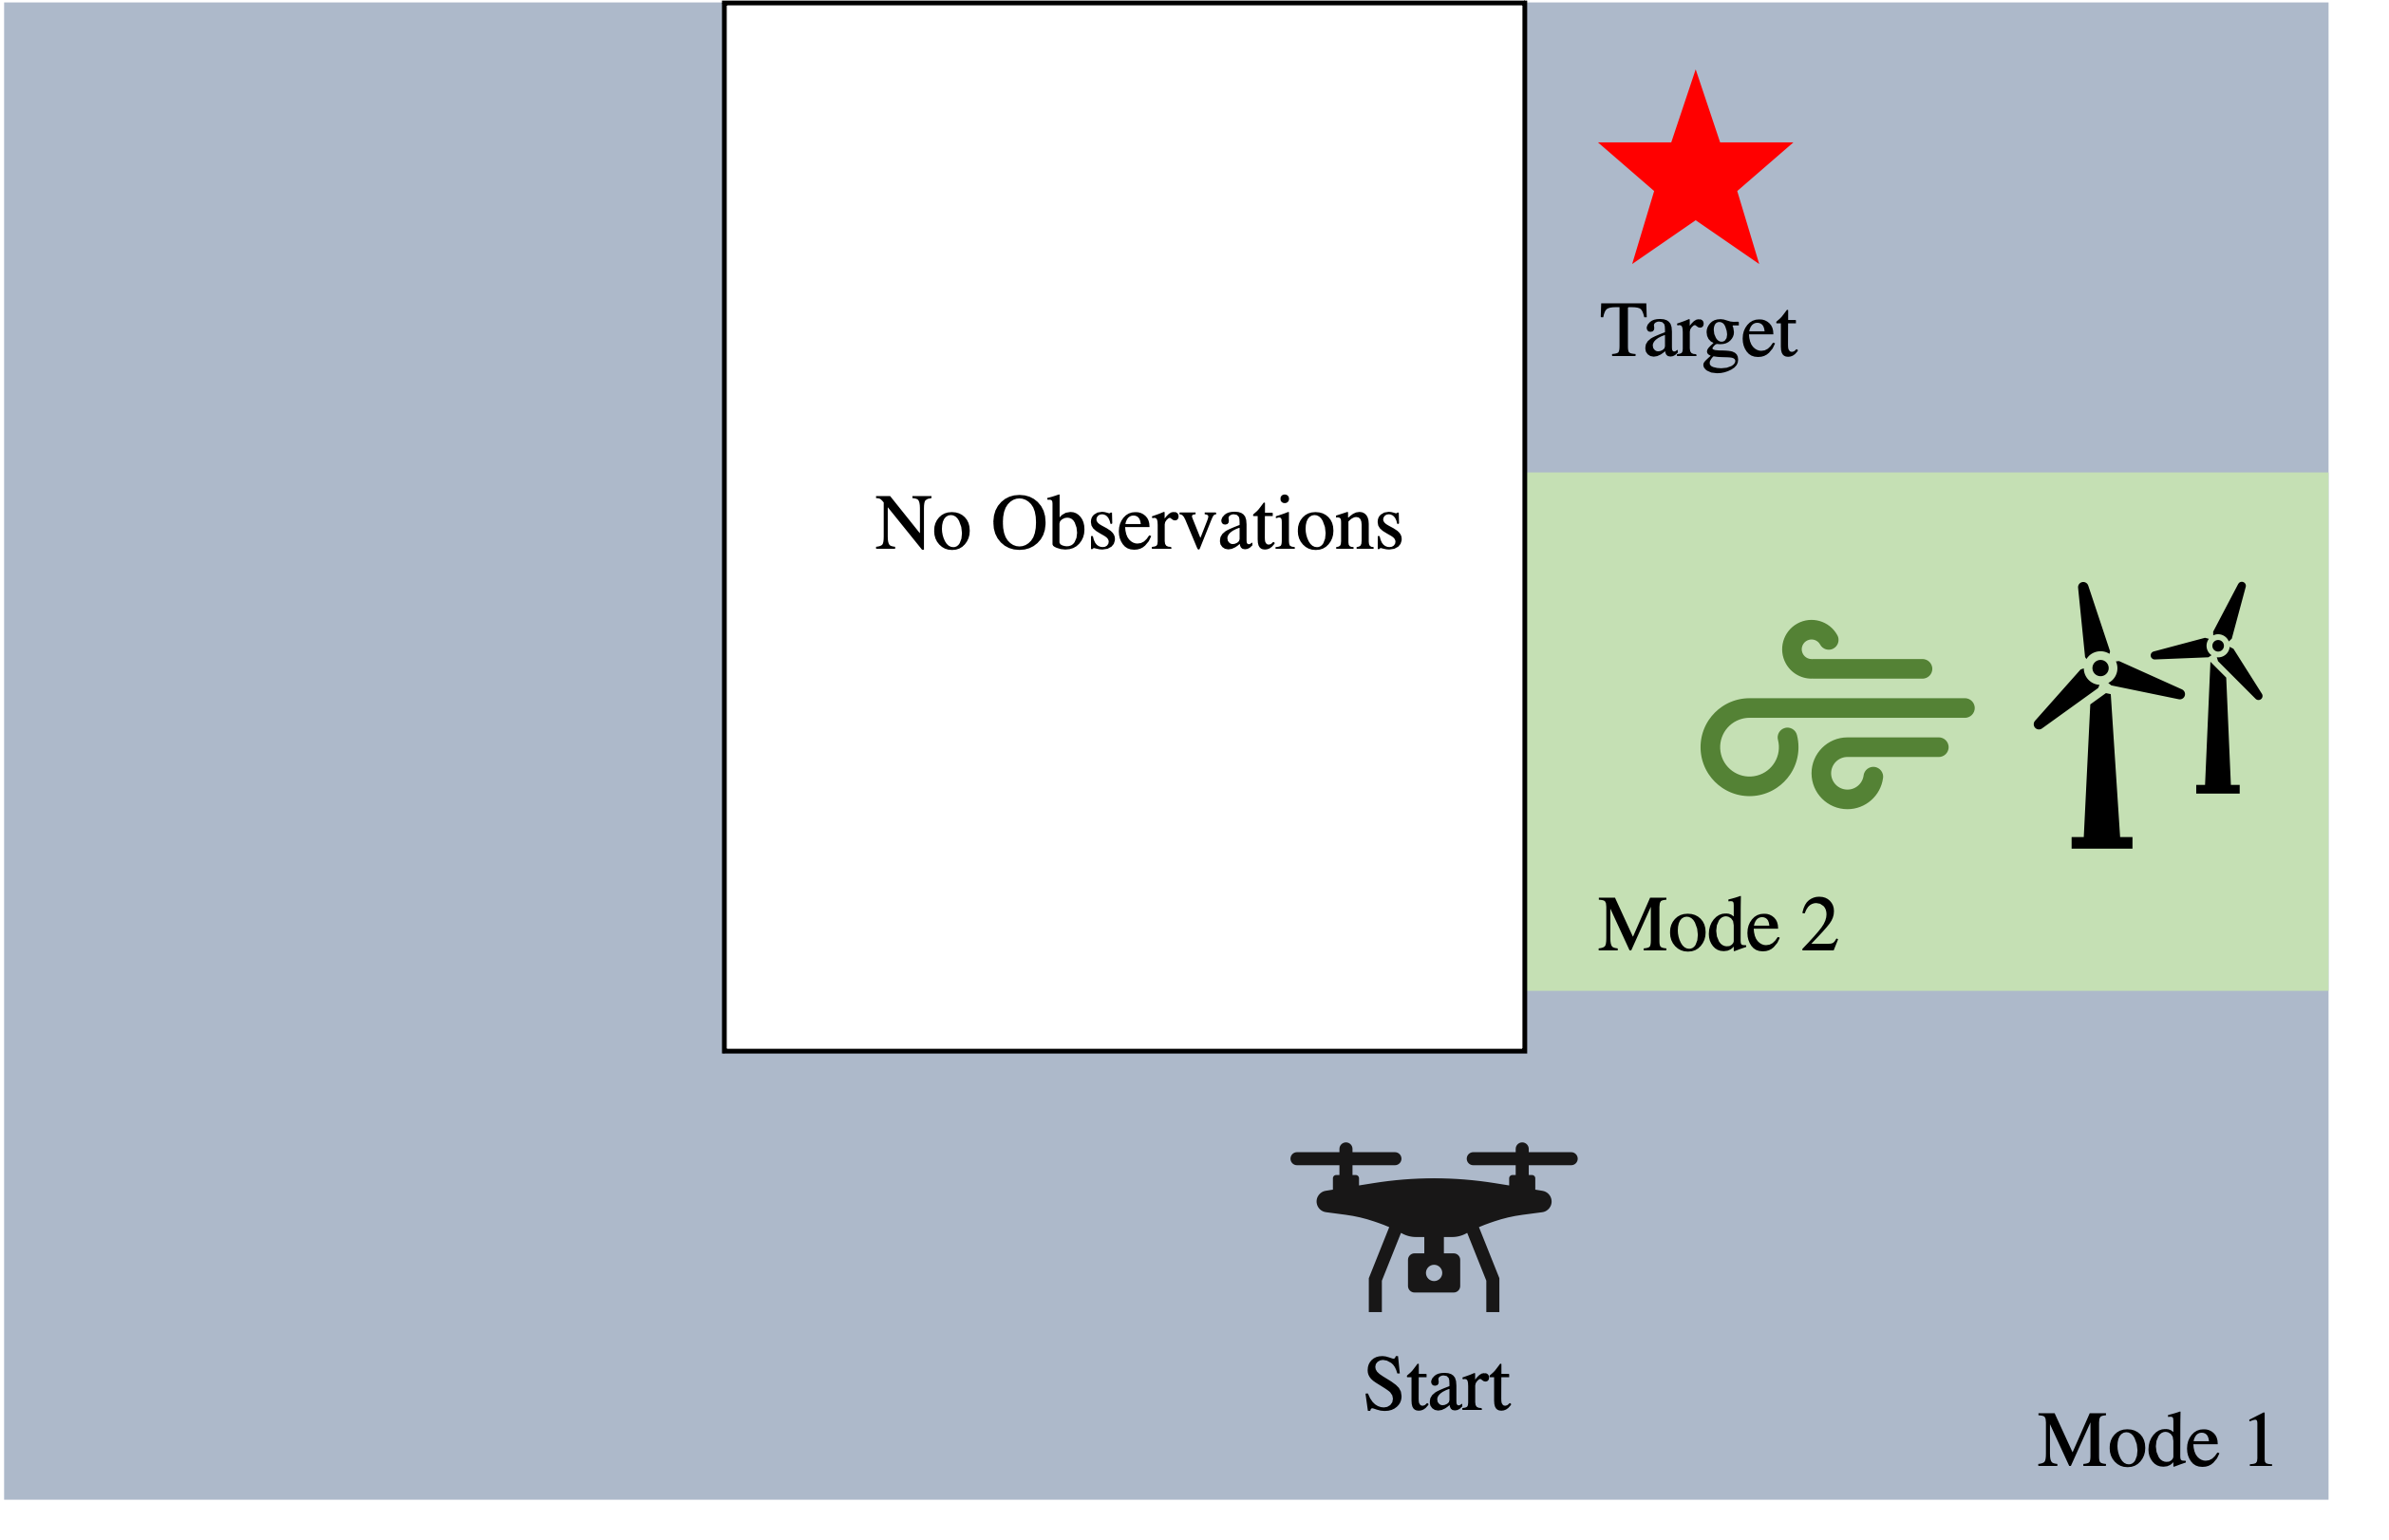
\includegraphics[width=1.0\textwidth]{./images/quadcopter-domain-collocation-ppt.png}
\caption[Quadcopter navigation problem]{\label{fig-problem-statement}\textbf{Quadcopter navigation problem}
Diagram showing a top-down view of an environment, representing a quadcopter subject to two dynamics modes:
1) an \textit{operable} dynamics mode away from the fan (blue) and 2) an \textit{inoperable}, turbulent dynamics mode in front of the fan (green).
The goal is to find trajectories from a start state $\state_0$, to the target state $\targetState$ (red star),
whilst avoiding the turbulent dynamics mode.}
\end{figure}
The state-space of the velocity controlled quadcopter example consists of the 2D Cartesian coordinates \(\state = (x, y)\)
and the controls consist of the speed in each direction, given by \(\control = (\velocity_x, \velocity_y)\).

\section{Contributions}
\label{sec:orgf038a1f}
This thesis explores methods for mode remaining control in multimodal dynamical systems that explicitly reason
about the uncertainties arising during learning and control.
The primary contributions of this thesis are as follows:
\begin{itemize}
\item \cref{chap-dynamics}: is concerned with learning representations of multimodal dynamical
systems, where both the underlying dynamics modes and how the system switches between them, are \emph{not fully known a priori}.
Motivated by learning dynamics models for model-based control, it formulates a probabilistic model
rich with latent spaces for control.
It then derives a variational inference scheme that principally handles uncertainty whilst providing scalability
via stochastic gradient methods.
The method is a \acrfull{mogpe} method with a \acrfull{gp}-based gating network.
\item \cref{chap-traj-opt-control}: investigates model-based control techniques that leverage the probabilistic model
from \cref{chap-dynamics} to solve the mode remaining navigation problem.
Due to the complexity of the problem, this chapter
assumes prior access to the environment, such that a data set of state transitions \(\mathcal{D}\) has
previously been collected and used to train the model. It presents three trajectory optimisation algorithms that
leverage the learned dynamics model's latent structure to solve the mode remaining navigation problem.
\item \cref{chap-active-learning}: then considers the more realistic scenario of not having prior access
to the environment. In this scenario, the agent does not have access to a historical data set for model learning.
Instead, it must actively explore its environment, collect data and use it to update its dynamics model,
whilst simultaneously attempting to remain in the desired dynamics mode.
It presents an exploration strategy for exploring multimodal dynamical systems whilst remaining in a
desired dynamics mode with high probability.
It then details how this exploration strategy can be combined with the methods from
\cref{chap-traj-opt-control,chap-dynamics} to solve the mode remaining navigation problem.
\end{itemize}

\section{Associated Publications}
\label{sec:orge827379}
The first trajectory optimisation algorithm presented in \cref{sec-traj-opt-collocation} and an initial
version of the approach for learning multimodal dynamical systems in \cref{chap-dynamics}, are published in:

{\color{BrickRed}\fullcite{scannellTrajectory2021}}

\chapter{Background and Related Work}
\label{sec:orgad7b40d}
\newcommand{\gpDomain}{\ensuremath{\mathcal{X}}}
\newcommand{\dynamicsModel}{\ensuremath{p_{\theta}}}
\newcommand{\constraintFunc}{\ensuremath{c}}
\newcommand{\safeSet}{\ensuremath{\mathcal{X}_{\text{feasible}}}}
The primary goal of this thesis is to control \emph{stochastic}, \emph{multimodal}, \emph{nonlinear} dynamical systems
to a target state, whilst remaining in the desired dynamics mode.
This is a \acrfull{soc} problem which can be summarised as follows:
\begin{displayquote}
\textit{For a given multimodal dynamical system with control inputs, determine a controller that
can navigate to a target state, whilst remaining in a desired dynamics mode.}
\end{displayquote}
This chapter formally defines this mode remaining navigation problem and reviews the relevant literature.
\section{Problem Statement \label{problem-statement-main}}
\label{sec:orgf9c3752}
Dynamical systems describe the behaviour of a system over time \(t\) and
are a key component of both control theory and \acrshort{rl}.
At any given time \(t\), a dynamical system has a state,
represented as a vector of real numbers \(\state_t \in \stateDomain \subseteq \R^{\StateDim}\).
The system can be controlled by applying control actions \(\mathbf{u}_t \in \controlDomain \subseteq \R^{\ControlDim}\)
at any given time.
This thesis considers \emph{stochastic}, \emph{multimodal}, \emph{nonlinear} dynamical systems, given by,
\begin{subequations} \label{eq-dynamics-main}
\begin{align}
\state_{\timeInd+1} &= \dynamicsFunc(\state_\timeInd, \control_\timeInd) + \bm\epsilon \\
&= \mode{\dynamicsFunc}(\state_\timeInd, \control_\timeInd) + \mode{\bm\epsilon}
\quad \text{if} \quad \modeVar(\state_{\timeInd})=\modeInd \nonumber \\
\mode{\bm\epsilon} &\sim \mathcal{N}(\mathbf{0}, \Sigma_{\mode{\bm\epsilon}}),
\end{align}
\end{subequations}
where the discrete mode indicator function
\(\alpha : \stateDomain \rightarrow \modeDomain\)
indicates which of the \(\ModeInd\) underlying dynamics modes
\(\{\mode{\latentFunc} : \mode{\stateDomain} \times \controlDomain \rightarrow \stateDomain \}_{\modeInd=1}^\ModeInd\),
and associated noise models
\(\mode{\bm\epsilon} &\sim \mathcal{N}\left(\mathbf{0}, \bm\Sigma_{\mode{\bm\epsilon}} \right)\),
governs the system at a given time step \(\timeInd\).
The output of the mode indicator function is referred to as the mode indicator variable and is given by
\(\alpha_{\timeInd} = \alpha(\state_{\timeInd}) \in \modeDomain = \{1,\ldots,\ModeInd\} = \mathbb{Z} \cap [1, \ModeInd]\).

This thesis assumes that the state \(\state\) is observed directly and is not subject to
observation noise.
This is a standard assumption in the \acrfull{mdp} framework, which is commonly adopted
in the \acrshort{rl} literature.
In this case, the \(\mode{\bm\epsilon}\) term solely represents the process noise,
which accounts for unwanted and, in general, unknown system disturbances.
For example, it is hard to model aerodynamic effects on aircraft, so these could be accounted
for in the process noise term.

\textbf{Optimal control}
Optimal control is a branch of mathematical optimisation that seeks to find a controller \(\pi\) that
optimises an objective function \(J_{\pi}(\x)\).
The objective function might be formulated to solve a particular task or to make the dynamical
system behave in a certain way.
Typically the goal is to minimise a cost function \(\costFunc : \stateDomain \times \controlDomain \rightarrow \R\).
This thesis considers the \emph{finite horizon problem}, given by,
\begin{align} \label{eq-optimal-control-objective}
J_{\pi}(\state) = &\E \left[ \sum_{\timeInd=0}^{\TimeInd} \costFunc(\state_{\timeInd}, \pi(\state_{\timeInd}, \timeInd))
\mid \state_0=\state \right]
\end{align}
where \(\TimeInd\) is known as the horizon.
The objective \(J_{\pi}(\state)\) quantifies the cost of deploying the controller \(\pi\) from
an initial state \(\state\).
The cost function typically consists of a terminal cost and a term which is integrated over the horizon (integral cost).
In a navigation task, the terminal cost may consist of the distance to the target, whilst the integral cost
may encode the notion of minimum effort control, e.g. energy consumption \citep{kirkOptimal2004}.

\textbf{Controller space}
The controller space \(\Pi\) defines the set of controllers over which optimisation is performed.
Controllers can have state feedback such that they are given by \(\control_t = \policy(\state_t)\).
These are closed-loop controllers and in the \acrshort{rl} literature are referred to as policies.
Alternatively, controllers can depend on time \(\control_t = \policy(t)\), in which case they are open-loop controllers.
This thesis considers the general case, given by \(\control_t = \policy(\state_t, t)\),
which encompasses both open-loop and closed-loop controllers.

\textbf{Mode remaining}
This thesis considers systems where the underlying dynamics modes are defined by disjoint state domains, i.e.
\(\mode{\stateDomain} = \{ \state \in \stateDomain \mid \modeVar(\state) = \modeInd \}\), with
\(\stateDomain_{i} \cap \stateDomain_{j} = \emptyset\) for distinct \(i, j \in \{1, \ldots \ModeInd\}\).
Notice that each mode's dynamics can leave their state space \(\mode{\stateDomain}\)
and enter another mode.
Ideally, this work seeks to enforce the controlled system to remain in a given mode.
Formally, a mode remaining controlled system is defined as follows.
\begin{definition}[Mode Remaining] \label{def-mode-remaining-main}
Let $\modeInd$ denote a dynamics mode, defined by its state domain $\mode{\stateDomain} \subseteq \stateDomain$.
Given an initial state $\state_0 \in \mode{\stateDomain}$, and a controller $\policy \in \Pi$,
the controlled system is said to be mode-remaining iff:
\begin{align} \label{eq-mode-remaining-def-main}
\dynamicsFunc(\state_{\timeInd}, \policy(\state_{\timeInd}, \timeInd))
&\in \mode{\stateDomain} \quad \forall \timeInd
\end{align}
\end{definition}

\begin{myquote}
\textbf{Mode remaining navigation problem}
Given this definition of a mode remaining controlled system, this thesis seeks to solve,
\begin{subequations} \label{eq-main-problem}
\begin{align}
\min_{\policy \in \Pi} \quad
%&J_{\pi}(\state_0) \\
&\E \left[ \sum_{\timeInd=0}^{\TimeInd} \costFunc(\state_{\timeInd}, \pi(\state_{\timeInd}, \timeInd)) \mid \state_0=\state_0 \right] \\
%&\E \left[ \sum_{\timeInd=0}^{\TimeInd} \costFunc(\state_{\timeInd}, \pi(\state_{\timeInd}, \timeInd))
%\mid \state_0=\state \right] \\
\text{s.t.} \quad &\state_{\timeInd+1} = \mode{\dynamicsFunc}(\state_\timeInd, \policy(\state_\timeInd, \timeInd)) + \mode{\bm\epsilon},
\quad \modeVar(\state_{\timeInd}) = \modeInd \quad &\forall \timeInd \in \{0, \ldots, \TimeInd-1\} \\
%&\text{\cref{eq-mode-remaining-def-explore}} \\
&\dynamicsFunc(\state_{\timeInd}, \policy(\state_{\timeInd}, \timeInd))
\in \desiredStateDomain \quad &\forall \timeInd \in \{0, \ldots, \TimeInd-1\} \\
%\modeVar_{\timeInd} = \desiredMode \quad \forall \timeInd \in \mathbb{Z} \cap [0,\TimeInd] \\
%&\state_{\timeInd} \in \desiredStateDomain \quad \forall \timeInd \in \mathbb{Z} \cap [0,\TimeInd] \\
&\state_{0} = \state_0 \\
&\state_\TimeInd = \targetState,
\end{align}
\end{subequations}
where $\targetState$ denotes the target state and $\desiredMode$ denotes the desired dynamics mode.
%and $J_{\pi}(\state_0)$ is the objective from \cref{eq-optimal-control-objective}.
\end{myquote}
% This is a constrained \acrfull{soc} problem with a terminal boundary condition.
Note that the objective function in \cref{eq-optimal-control-objective} is not of primary interest in this work.
The novelty of this work arises from remaining in the desired dynamics mode \(\desiredMode\).

\section{Optimal Control \label{sec-optimal-control}}
\label{sec:org66a8fc1}
\begin{figure}[!t]
\centering
\begin{tikzpicture}[
squarednode/.style={rectangle, fill=teal!7, width=2cm},
blanknode/.style={rectangle, width=2cm}
]

\node[squarednode, align=center] (agent)                             {Controller / Agent\\$\pi(\state_t, t)$};
\node[blanknode, align=center] (control)    [below right=of agent]  {Control / Action $\control_t$};
\node[blanknode, align=left] (cost)      [below left=of agent]   {Cost / negative reward $\costFunc(\state_t, \control_t)$\\Next state $\state_{t+1}$};
\node[squarednode, align=center] (env)       [below left=of control] {System / Environment\\$f(\state_t, \control_t)$};

\draw[--] (agent) -| (control);
\draw[->] (control) |- (env);
\draw[--] (env) -| (cost);
\draw[->] (cost) |- (agent);
\end{tikzpicture}
\caption[\acrfull{mdp}]{\textbf{\acrfull{mdp}} Illustration of an \acrshort{mdp} through the lens of optimal control. The controller (agent) uses all past knowledge, absorbed into the previous state $\state_t$ (Markov property), to decide which control (action) $\control_t$ to execute. It then observes the next state $\state_{t+1}$ and the cost (negative reward) associated with the state transition. The cost function is assumed to be known. The agent's goal is to minimise the cumulative cost (maximise the cumulative reward).}
\label{fig-mdp}
\end{figure}
The discrete-time optimal control problem considered in this thesis can be modelled as a
\acrfull{mdp}, as seen in \cref{fig-mdp}.
The \acrshort{mdp} framework refers to the controller \(\pi\) as the agent, the control \(\control\)
as the action, and the dynamical system \(f\) as the environment.
Further to this, the goal is to maximise the cumulative reward instead of minimising the cumulative cost.
However, slight manipulation of the objective enables cost and reward functions to be interchanged.
The key idea in \acrshort{mdp}s is that all past information is represented by the current state \(\state_t\),
which is known as the Markov property.
In this thesis, most work is formulated through the lens of optimal control.
However, the controller is sometimes referred to as the agent and the system is often referred to
as the environment.

In general, solutions to optimal control problems can be characterised by two different approaches,
Pontryagin's Minimum Principe \citep{pontryagin1987mathematical} (based on the calculus of variations)
and Bellman's Minimum Principle \citep{bellmanDynamic1956}.
Although Pontryagin's Minimum Principle offers computational benefits over Bellman's principle, it does not
readily generalise to the stochastic case.
For this reason, we restrict our discussion to Bellman's principle and the solution arising from it, known as
dynamic programming.

\subsection{Dynamic Programming}
\label{sec:org3e2bb4e}
Dynamic programming \citep{bellmanDynamic1956} encompasses a large class of algorithms that can be
used to find optimal controllers given a model of the environment as an \acrshort{mdp}.
However, classical dynamic programming algorithms are of limited use as they rely on
accurate dynamics models and have a significant computational expense.
Nevertheless, they are still important theoretically.
The main idea of dynamic programming (and \acrshort{rl} in general) is to structure the search for good controllers using
value functions \(V\).
Optimal controllers can easily be found from optimal value functions \(V_*\), which satisfy the Bellman
optimality equations,
\begin{align} \label{eq-bellman}
V_*(\state) = \min_{\control} &\E \left[ \underbrace{\costFunc(\state_{\timeInd}, \pi(\state_{\timeInd}, \timeInd))}_{\text{first step}}
+ \underbrace{V_*(f(\state_{t}, \pi(\state_{t}, t)))}_{\text{future}}
\mid \state_0=\state \right].
\end{align}
In the finite horizon setting, directly solving the Bellman equations backwards in time is referred to
as dynamic programming.

Approximate dynamic programming encompasses a large class of methods that, given a controller \(\pi\),
approximate the value function \(V_{\pi}(\state)\) for each state \(\state\) with a parameterised function.
The approximate value function can then be used for \emph{policy improvement}, where a controller
with superior performance is computed.
In general, approximate dynamic programming is a large collection of algorithms that encompasses methods from
\acrshort{rl} as well.
However, these methods are out of the scope of this thesis.

\subsection{Reinforcement Learning}
\label{sec:orga74f2f9}
There are multiple approaches to finding controllers \(\pi\) that minimise the expected cost
in \cref{eq-optimal-control-objective} subject to the stochastic dynamics in \cref{eq-dynamics-main}.
However, a central assumption of many methods is that both the system dynamics and cost function are \emph{known a priori}.
In contrast, we consider problems where
the underlying dynamics modes \(\{\mode{\dynamicsFunc}\}_{\modeInd=1}^{\ModeInd}\)
and how the system switches between them \(\modeVar\), are \textit{not fully known a priori}.
Further to this, the problem statement in \cref{eq-main-problem} contains a mode remaining constraint,
which requires explicit knowledge of the desired dynamics mode and its state domain.

To apply control and planning techniques in systems with unknown dynamics,
system identification emerged as a set of techniques for computing unknown parameters, e.g. mass of a component
\citep{ljungSystem1999}.
This is a two-staged approach which first learns about the environment and then uses this
learned model to find the optimal controller.
However, this approach learns about the environment globally and often incurs high costs during system identification.

\acrfull{rl} provides the most general framework for extending optimal
control to problems with incomplete knowledge of the system dynamics.
The classic text by \cite{sutton2018reinforcement} gives a general introduction to \acrshort{rl}.
The main goal is to learn good behaviours from interactions with an environment.
Typically this is in the form of a state feedback controller, known as a policy, which makes an agent's interaction
with the environment closed-loop.
In contrast to the system identification approach,
the goal of \acrshort{rl} is to minimise costs (maximise rewards) during the learning process.
Further to this, \acrshort{rl} only needs to learn about the states relevant to solving
the optimal control problem.

\begin{algorithm}[!t]
\caption{\acrfull{mbrl}}\label{alg-mbrl-background}
\begin{algorithmic}[1]
\Require{Policy/controller $\policy_0$, dynamics model $\dynamicsModel$, start state $\state_0$}
\For{$i = 0, 1,  \ldots $}
    \State Select $\pi_i$ using exploration strategy, e.g. \cref{eq-greedy-exploration}
    \State Collect environment data set $\dataset_i$ using $\pi_i$; add to dataset $\dataset_{0:i} = \{\dataset_{i} \cup \dataset_{0:i-1}\}$
    \State Update dynamics model $\dynamicsModel$ using $\dataset_{0:i}$.
\EndFor
\end{algorithmic}
\end{algorithm}

\subsubsection{Model-based Reinforcement Learning}
\label{sec:orgf65325c}
This thesis is interested in a subset of \acrshort{rl} known as \acrfull{mbrl}.
It solves the optimal control problem in \cref{eq-optimal-control-objective}
by first learning a dynamics model and then using this learned model with model-based control techniques.
As both \acrfull{mfrl} and \acrshort{mbrl} methods learn models,
the model in the name refers to the dynamics model \(f\), as  \acrshort{mfrl} approaches do not learn
representations of the dynamics \(f\).
\cref{alg-mbrl-background} illustrates a common \acrshort{mbrl} procedure where an agent incrementally explores
its environment, collecting data \(\mathcal{D}_i\) at each iteration \(i\) and
updating its dynamics model \(\dynamicsModel\).


As more systems are becoming data-driven, learning dynamics models for model-based control has shifted to
needing task-centric methods that simultaneously learn about the environment, whilst optimising a controller
to obtain low cumulative costs.
The field of \acrshort{mbrl} seeks to solve many optimal control problems by incrementally learning a dynamics model
in this way \citep{deisenrothPILCO2011,chuaDeep2018}.
\acrshort{mbrl} shares similarities with the system identification and control process,
except that the dynamics learning and control are updated simultaneously.
There are two main components to a \acrshort{mbrl} algorithm: 1) a method for learning a dynamics
model \(\dynamicsModel\) and 2) a controller (or policy) \(\pi\) that leverages the learned dynamics model \(\dynamicsModel\).
The controller may be a parameterised state feedback controller (policy) \(\pi\), which is trained using
\acrshort{mfrl} algorithms and the learned dynamics model.
Alternatively, the controller may take the form of a model-based control algorithm such as \acrfull{mpc}.

\subsection{Model-based Control and Planning}
\label{sec:orgee5f9cb}
This section reviews model-based control methods that leverage learned dynamics models in the \acrshort{mbrl} setting.
In the \acrshort{rl} literature, model-based control is often referred to as planning.
The work in this thesis is primarily focused on model-based control techniques,
in particular, trajectory optimisation.

\textbf{Trajectory optimisation}
Instead of approximating a value function or a policy, it is possible to directly optimise the controls
\(\controlTraj = \{\control_1, \ldots, \control_{T-1} \}\) over a horizon \(T\).
This is known as trajectory optimisation and is given by,
\begin{subequations} \label{eq-trajectory-optimisation}
\begin{align}
\controlTraj =
\argmin_{\controlTraj} &\E \left[ \sum_{\timeInd=0}^{\TimeInd} \costFunc(\state_{\timeInd}, \control_{\timeInd})
\mid \state_0=\state \right] \\
&\text{s.t. } \quad \state_{t+1} = f(\state_t, \control_t) + \epsilon,
\end{align}
\end{subequations}
which finds an optimal sequence of controls \(\controlTraj\) for a given start state \(\state_0\).
Many recent works have used trajectory optimisation with learned dynamics models.
For example, \cite{nakkaChanceConstrained2021} developed a chance-constrained trajectory optimisation
algorithm that leverages a dynamics model learned using a robust regression model.
\cite{rybkinModelBased2021} utilise a latent space dynamics model -- learned
with a convolutional neural network for the encoder and a recurrent neural network for the dynamics -- which scales to high-dimensional inputs such as images.
In \acrshort{mbrl}, trajectory optimisers often exploit inaccuracies of the learned dynamics model.
\cite{boneyRegularizing2019} propose a trajectory optimisation approach that relives this exploitation by
learning the dynamics using a denoising autoencoder.
The resulting trajectory optimisation algorithm avoids regions of the learned dynamics model where no data
has been observed.

\textbf{Model predictive control}
Instead of directly applying the control inputs found with trajectory optimisation in an open-loop fashion,
it is possible to obtain a closed-loop controller.
This is achieved by iteratively applying the first control \(\control_0\) and resolving the trajectory optimisation
problem in \cref{eq-trajectory-optimisation},
\begin{subequations} \label{eq-mpc-loop}
\begin{align}
\pi_{\text{MPC}}(\state) =
\arg \min_{\control_0}
\min_{\controlTraj} &\E \left[ \sum_{\timeInd=0}^{\TimeInd} \costFunc(\state_{\timeInd}, \control_{\timeInd})
\mid \state_0=\state \right] \\
&\text{s.t. } \quad \state_{t+1} = f(\state_t, \control_t) + \epsilon,
\end{align}
\end{subequations}
This is known as \acrfull{mpc} \citep{eduardof.Model2007}.
However, in practice, it is often too computationally expensive to obtain real-time control with \acrshort{mpc}.
Many approximate solutions have been introduced in the literature, that seek to balance the computational complexity
and accuracy trade-off differently \citep{bettsSurvey1998}.

For example, \acrfull{ilqr} can generate trajectories for nonlinear systems by
iteratively approximating the dynamics to be linear around a nominal trajectory and optimising for the controls.
\acrshort{ilqr} works well for quadratic cost functions but can be used with any cost function by approximating the cost
function with a second-order Taylor expansion.
However, in this case, \acrshort{ilqr} is susceptible to converging
to terrible (local) optima if the true cost function is highly non-convex.
\cite{boedeckerApproximate2014} present a real-time \acrshort{ilqr} controller based on sparse \acrshort{gps}.
\cite{rohrProbabilistic2021} propose a novel \acrshort{lqr} controller synthesis for
linearised \acrshort{gp} dynamics that yields robust controllers with respect to a probabilistic stability margin.

\acrshort{mpc} has directly been used with ensembles of probabilistic neural networks \citep{chuaDeep2018,nagabandiDeep2020}
and with \acrshort{gps} \citep{kamtheDataEfficient2018}.
\cite{lambertLowLevel2019} control a quadcopter using online \acrshort{mpc} and a dynamics model learned using
probabilistic neural networks.

\textbf{Offline trajectory optimisation}
Instead of solving the trajectory optimisation problem in \cref{eq-trajectory-optimisation} online,
it can be solved offline.
For example, the state-control trajectory can be found offline and used as a reference trajectory
for a tracking controller.
Alternatively, the trajectory optimiser can be used offline to learn a state feedback controller (policy)
using guided policy search \citep{levineGuided2013}.

\subsection{Constrained Control}
\label{sec:org4c36f66}
This work aims to control multimodal dynamical systems subject to the mode remaining
constraint in \cref{eq-main-problem}.
However, neither the underlying dynamics modes nor how the system switches between them, are \emph{known a priori}.
To this end, this thesis is interested in model-based control techniques which can
learn and enforce latent constraints.

It is common to require constraints on the states \(\state\) and controls \(\control\) of a controlled system.
For example, an autonomous system may wish to remain in a subset of its state space where it knows its dynamics model
is valid.
The system may also be subject to constraints on the controls due to physical limitations, e.g.
how quickly a quadcopter can accelerate and turn.
Constraints of this type can be encoded via inequality constraints on the states \(\state\) and controls \(\control\),
\begin{align} \label{eq-}
&\constraintFunc_\state(\state_\timeInd) \geq 0, \quad \forall \timeInd \geq 0, \\
&\constraintFunc_\control(\control_\timeInd) \geq 0, \quad \forall \timeInd \geq 0.
\end{align}
The feasible regions of these constraints can be written as sets,
\begin{align} \label{eq-}
\stateDomain_{\text{feasible}} = &\{ \state \in \R^\StateDim \mid \constraintFunc_\state(\state) \geq 0 \}, \\
\controlDomain_{\text{feasible}} = &\{ \control \in \R^\ControlDim \mid \constraintFunc_\control(\control) \geq 0 \},
\end{align}
so the constraints can alternatively be written as,
\begin{align} \label{eq-}
\state_\timeInd &\in \stateDomain_{\text{feasible}}  \quad \forall t \geq 0 \\
\control_\timeInd &\in \controlDomain_{\text{feasible}} \quad \forall t \geq 0.
\end{align}
For a parametric controller \(\policy\), the control constraints can be encoded directly into the controller by
parameterising it so that its range is restricted to \(\controlDomain_{\text{feasible}}\),
i.e. \(\policy(\state_\timeInd) \in \controlDomain_{\text{feasible}}\),
for all \(\state \in \stateDomain_{\text{feasible}}\).
The state constraints can be enforced by ensuring that the set \(\StateDomain\) is forward invariant.
\begin{definition}[Forward invariant]
Given a dynamical system $\state_{t+1} = f(\state_t, \pi(\state_t, t))$,
a set $\safeSet$ is \textbf{forward invariant} under the controller $\pi \in \Pi$, iff, for all $\state_0 \in \safeSet$,
all future states remain in the set, i.e.  $f(\state_t, \pi(\state_t, t)) \in \safeSet \quad \forall t$.
%The system is safe with respect to the set $\safeSet$ if the set is \textbf{forward invariant}.
\end{definition}
There are multiple approaches to enforcing state constraints via invariant sets.
Two common approaches are
Lyapunov functions \citep{lyapunovGeneral1992a} and control barrier functions \citep{amesControl2019}.
Lyapunov functions are more restrictive than control barrier functions as they provide stability guarantees
which are not a necessary condition to render \(\stateDomain_{\text{feasible}}\) forward invariant.
Although these are interesting directions for future work, they are out of the scope of this thesis.

\textbf{Unknown constraints}
This work is interested in learning constraints whilst ensuring that they are satisfied.
\cite{ariafarADMMBO2019,gelbartBayesian2014} introduce algorithms to minimise an unknown objective
(Bayesian optimisation) subject to unknown constraints.
\cite{sadighSafe2016} propose an \acrshort{mpc} method that satisfies \emph{a priori unknown} constraints with high probability.
However, they do not deploy a strategy to actively learn about the constraints.
In contrast, \cite{schreiterSafe2015} consider safe exploration for active learning.
They distinguish safe and unsafe regions with a binary \acrshort{gp} classifier, which is
learned separately to the dynamics model. Their exploration strategy then considers
the differential entropy of the dynamics \acrshort{gp} and they use the \acrshort{gp} classifier to define
a set of safety constraints.

\textbf{Stochastic constraints}
In stochastic systems it is not possible to make deterministic statements about constraints.
This is because given a start state \(\state_0\) the resulting trajectories are random variables.
Therefore, the constraints \(\constraintFunc_{\state}(\state)\) are also random variables.
To reason about constraints in stochastic systems, we need a method to measure uncertainty in this
random variable.

A simple approach is to consider expected constraints \(\E[\constraintFunc_{\state}(\state)]\).
However, although expected performance is a reasonable objective, expected constraints make less sense.
For example, although the expected constraints \(\E[\constraintFunc_{\state}(\state)]\) hold, a system may
still violate them frequently if the constraints variance \(\V[\constraintFunc_{\state}(\state)]\) is high.
\cite{ferberGames1958} proposed risk sensitivity which uses higher-order moments as well as the expected value.
Value at risk \citep{duffieOverview1997a} is an even stronger notion, which guarantees constraint satisfaction
with high probability.

\acrshort{mpc} \citep{eduardof.Model2007} is the most direct method to embed constraints.
At each time step, \acrshort{mpc} ensures that the constraints hold over a given horizon.
However, it is worth noting that these constraints still cannot be guaranteed in stochastic systems.
For stochastic systems, \cite{schwarmChanceconstrained1999} proposed to satisfy constraints with high probability.
Such constraints are named chance constraints.
Chance constraints are applicable in systems where the uncertainty arises from learning from observations.
i.e. they are applicable with latent constraints.

\section{Learning Dynamical Systems for Control}
\label{sec:orgdd03c10}
This section reviews methods for learning representations of dynamical systems for control.
When learning representations of dynamical systems from observations it is important to consider the different
forms of uncertainty.
For example, when using a learned model for control, it is important to \emph{know what we do not know}.
This knowledge can be used to encode \emph{risk-sensitive} control (avoid regions where the model cannot predict confidently)
or to guide exploration.
\cref{sec-unc-exploration} discusses exploration strategies that leverage well-calibrated uncertainty estimates.

\subsection{Sources of Uncertainty}
\label{sec:orgfdf0a23}
This section characterises the uncertainty that arises in \acrshort{rl}.

\textbf{Aleatoric uncertainty}
Dynamical systems give rise to temporal observations arriving as a sequence
\(\stateTraj = \{\state_1, \ldots, \state_\TimeInd\}\).
These measurements are often corrupted by (observation) noise due to imperfections in the measurement process.
Even when it is known that there is uncertainty in the measurement process, there still remains uncertainty about its
form.
Given our current understanding of the real-world, many dynamical systems also appear to be inherently stochastic.
This is due to our inability to model certain phenomena accurately  (e.g. turbulence).
Stochasticity arising from state transitions in this way is known as process noise.
Observation and process noise are the constituent sources of \emph{aleatoric uncertainty};
uncertainties that are inherent in a system and cannot be reduced.

\textbf{Epistemic uncertainty}
The uncertainty arising from learning the dynamics \(f\) from observations is known as \emph{epistemic uncertainty}.
For example, we may be uncertain about the structure of the model or the value of specific
model parameters \(\theta\).
This type of uncertainty accounts for those we could know, but we do \emph{not know a priori}.
As such, \emph{epistemic uncertainty} can be reduced by exploring, collecting data and updating the model with
this new experience.

Distinguishing these two sources of uncertainty is important in \acrshort{rl}.
For example, the \emph{epistemic uncertainty} is useful for guiding exploration into regions
of the system that have not been observed.
In turn, this data can be used to reduce the model's \emph{epistemic uncertainty} by updating the model.
In contrast, driving the system into regions of the model with high \emph{aleatoric uncertainty} is not desirable.
Consider the case where the model is confident that the system is subject to high process noise in a particular region.
Guiding the system into this region will not reduce the model's \emph{epistemic uncertainty} because the model
has already been trained on data from this region.
Further to this, it may be undesirable to enter regions of
high \emph{aleatoric uncertainty} because they may result in poor performance or even catastrophic failure.

\subsection{Learning Single-Step Dynamics Models}
\label{sec:org5a5e349}
This work considers single-step dynamics models with the delta state formulation,
which regularises the predictive distribution, given by
\(\state_{\timeInd+1} &= \state_\timeInd + \dynamicsFunc(\state_\timeInd, \control_\timeInd) + \bm\epsilon\).
Although multi-step dynamics models are an interesting direction for learning-based control, they are
out of the scope of this thesis.

Single-step dynamics models have been deployed in a large variety of learning-based control algorithms.
Early approaches include using single-step linear models \citep{schneiderExploiting1996} and
single-step \acrshort{gp} models
\citep{deisenrothPILCO2011,vinogradskaStability2016,rohrProbabilistic2021,hewingLearningBased2020,kollerLearningBased2018}
for low-dimensional control problems.
More recently, single-step dynamics models have been learned using neural networks.
For example, \citep{chuaDeep2018,jannerWhen2019,kurutachModelEnsemble2018} use ensembles
of neural networks and \citep{depewegLearning2017,galImproving2016} use Bayesian neural networks
with parametric uncertainty.

\textbf{Probabilistic models}
\emph{Mathematical models} are compact representations (sets of assumptions) that attempt to capture key features of the
phenomenon of interest in a precise mathematical form.
Probabilistic modelling provides the capability of constructing \emph{mathematical models}
that can represent and manipulate uncertainty in data, models, decisions and predictions.
As such, linking observed data to underlying phenomena through probabilistic models
is an interesting direction for modelling, analysing and controlling dynamical systems.
It enables the uncertainty to be represented and manipulated;
it provides a systematic way to combine observations with existing knowledge via a \emph{mathematical model}.
Learning representations of dynamical systems for control using probabilistic models has shown much promise.
Moreover, learning single-step dynamics models that quantify uncertainty has been central to
recent successes in \acrshort{mbrl} \citep{chuaDeep2018,jannerWhen2019}.

Modelling a Bayesian belief over the dynamics function \(f\) provides a principled method for modelling
\emph{epistemic uncertainty} arising from learning from data, through the posterior distribution.
\acrshort{gps} are the state-of-the-art approach for Bayesian nonparametric regression and
are a building block for the methods presented in this thesis.
\acrshort{gps} have become a popular choice for learning representations of dynamical systems
\citep{nguyen-tuongModel2009,buisson-fenetActively2020,wangSafe2018}
and have been used for both \acrshort{rl}
\citep{deisenrothPILCO2011,doerrOptimizing2017,vinogradskaNumerical2020,polymenakosSafe2019}
and for \acrshort{mpc}
\citep{kollerLearningBased2018,hewingCautious2020,hewingLearningBased2020,kollerLearningBased2018,kamtheDataEfficient2018}.

\subsection{Gaussian Processes}
\label{sec:org71ee188}
The mathematical machinery underpinning \acrshort{gps} is now detailed.

\textbf{Multivariate Gaussian identities}
Inference techniques with \acrshort{gps} leverage multivariate Gaussian conditioning operations.
As such, introducing the multivariate Gaussian identities is a natural place to start.

Gaussian distributions are popular in machine learning and control theory. This is not only due to their
natural emergence in statistical scenarios (central limit theorem) but also their intuitiveness and
mathematical properties that render their manipulation tractable and easy.

Consider a multivariate Gaussian whose random variables are partitioned into two vectors \(\f\) and \(\u\).
The joint distribution takes the following form,
\begin{align*} \label{eq-joint-gaussian}
\left[\begin{array}{c}
      \f \\
      \u
\end{array}\right]
\sim\ &\mathcal{N}\left(
\left[\begin{array}{c}
      \bm\mu_{\f} \\
      \bm\mu_{\u}
 \end{array}\right]
\left[\begin{array}{cc}
      \bm\Sigma_{\f\f} & \bm\Sigma_{\f\u} \\
      \bm\Sigma_{\u\f} & \bm\Sigma_{\u\u}
 \end{array}\right]\right),
\end{align*}
where \(\bm\mu_{\f}\) and \(\bm\mu_{\u}\) represent the mean vectors, \(\bm\Sigma_{\f\f}\) and \(\bm\Sigma_{\u\u}\)
represent the covariance matrices,
and \(\bm\Sigma_{\u\f}\) and \(\bm\Sigma_{\f\u}\) represent the cross-covariance matrices.
The marginalisation property of Gaussian distributions states that for two jointly Gaussian random variables,
the marginals are also Gaussian,
\begin{align} \label{eq-gaussian-marginal}
p(\f) &= \int p(\f, \u) \text{d}\u = \mathcal{N} \left(\f \mid \bm\mu_{\f}, \bm\Sigma_{\f\f} \right), \\
p(\u) &= \int p(\f, \u) \text{d}\f = \mathcal{N} \left(\u \mid \bm\mu_{\u}, \bm\Sigma_{\u\u} \right).
\end{align}
Conveniently, the conditional densities are also Gaussian,
\begin{align} \label{eq-gaussian-conditional}
\f \mid \u &\sim \mathcal{N} \left(\bm\mu_{\f} + \bm\Sigma_{\f\u} \bm\Sigma_{\u\u}^{-1}(\u - \bm\mu_{\u}), \bm\Sigma_{\f\f} - \bm\Sigma_{\f\u}\bm\Sigma_{\u\u}^{-1}\bm\Sigma_{\u\f} \right), \\
\u \mid \f &\sim \mathcal{N} \left(\bm\mu_{\u} + \bm\Sigma_{\u\f} \bm\Sigma_{\f\f}^{-1}(\f - \bm\mu_{\f}), \bm\Sigma_{\u\u} - \bm\Sigma_{\u\f}\bm\Sigma_{\f\f}^{-1}\bm\Sigma_{\f\u} \right).
\end{align}
Consider the case where \(\u\) represents some observations and \(\f\) represents a new test location.
\cref{eq-gaussian-conditional} can be used to make
inferences in the location \(\f\) given the observations \(\u\), i.e. make
sophisticated interpolations on the measurements based on their closeness.
In real-world scenarios, it is desirable to consider the entire input domain, instead of simply
pre-selecting a discrete set of locations.
Gaussian processes provide this mathematical machinery.


\textbf{Gaussian processes}
Informally, \acrshort{gps} are a generalisation of the multivariate Gaussian distribution, indexed by an
input domain as opposed to an index set.
Similar to how a sample from an \(N-\text{dimensional}\) multivariate Gaussian is an \(N-\text{dimensional}\) vector,
a sample from a \acrshort{gp} is a random function over its domain.
Formally, a \acrshort{gp} is defined as follows,
\begin{definition}[Gaussian process]
A \acrfull{gp} is a collection of random variables, any finite number of which
have a joint Gaussian distribution \citep{rasmussenGaussian2006}.
\end{definition}

More intuitively, a Gaussian process  is a distribution over functions \(f(\cdot): \gpDomain \rightarrow \R\)
defined over an input domain \(\gpDomain \in \R^{D_f}\).
Whilst Gaussian distributions represent distributions over finite-dimensional vectors, \acrshort{gps} represent
distributions over infinite-dimensional functions.
A \acrshort{gp} is fully defined by a mean function \(\mu(\cdot) : \gpDomain \rightarrow \R\) and a covariance
function \(k(\cdot, \cdot) : \gpDomain \times \gpDomain \rightarrow \R\) (also known as a kernel),
\begin{align} \label{eq-gp-mean-cov}
f(\cdot) &\sim \mathcal{GP}\left(\mu(\cdot), k(\cdot,\cdot) \right), \\
\mu(\cdot) &= \E[f(\cdot)], \\
k(\cdot, \cdot') &= \E[(f(\cdot) -\mu(\cdot)) (f(\cdot') - \mu(\cdot'))].
\end{align}
Importantly, for a given set of training inputs from the
functions domain \(~{\mathbf{X} = \{ \mathbf{x}_1, \ldots, \mathbf{x}_N \}}\), the associated function values
\(\mathbf{f} = \{f(\mathbf{x}_1), \ldots, f(\mathbf{x}_N) \}\),
are jointly Gaussian.
This results in an \(N-\text{dimensional}\) multivariate Gaussian random variable \(\mathbf{f}\), given by,
\begin{equation} \label{eq-gp-marginal}
\mathbf{f} \sim \mathcal{N}(\mu(\mathbf{X}), k(\mathbf{X}, \mathbf{X})).
\end{equation}
\begin{myquote}
A common kernel that is used throughout this thesis is the Squared Exponential
kernel with \acrfull{ard}, given by,
\begin{equation} \label{eq-se-kernel}
k(x, x') = \sigma_f^2 \exp\left(-\frac{1}{2} \sum_{d=1}^{D_f} \left( \frac{x_{d}- x'_{d}}{l_d} \right)^2 \right),
\end{equation}
where $\sigma_f^2$ represent the signal variance and $l_d$ is a lengthscale parameter associated with
input dimension $d$.
The lengthscale parameter determines the length of the "wiggles" in the function and
the signal variance $\sigma_f^2$ determines the average deviation of the function from its mean.
\end{myquote}
Given mean and kernel functions with parameters \(\bm\theta\), the marginal distribution is given by,
\begin{equation} \label{eq-gp-prior}
p(\mathbf{f} \mid \mathbf{X}) = \mathcal{N}(\mathbf{f} \mid \mu(\mathbf{X}), k(\mathbf{X}, \mathbf{X})).
\end{equation}
where the dependency on the parameters \(\bm\theta\) has been dropped, i.e.
\(p(\f \mid \mathbf{X}) = p(\f \mid \mathbf{X}, \bm\theta)\).
This simplification will be used throughout this thesis for notational conciseness.
By definition, these observations \(\mathbf{f}\) are jointly Gaussian with any un-observed function value
\(f_* = f(\mathbf{x}_*)\) at a new test input,
\begin{align*} \label{eq-gp-joint}
\left[\begin{array}{c}
      \mathbf{f} \\
      f^{*}
\end{array}\right]
\sim\ &\mathcal{N}\left(
\left[\begin{array}{c}
      \mu(\mathbf{X}) \\
      \mu(\mathbf{x}_{*})
 \end{array}\right]
\left[\begin{array}{cc}
      k(\mathbf{X}, \mathbf{X}) & k(\mathbf{X},\mathbf{x}_{*}) \\
      k(\mathbf{x}_{*},\mathbf{X}) & k(\mathbf{x}_{*},\mathbf{x}_{*})
 \end{array}\right]\right).
\end{align*}
Given the multivariate Gaussian conditionals in \cref{eq-gaussian-conditional}, it is easy to see how
the distribution over the test function value \(f_*\),
can be obtained by conditioning on the observations,
\begin{align} \label{eq-gp-prediction}
p(f_{*} \mid \mathbf{x}_*, \mathbf{f}, \mathbf{X}) &= \mathcal{N}(f_* \mid \mu, \sigma^2)  \\
\mu &= \mu(\mathbf{x}_*) + k(\mathbf{x}_*, \mathbf{X}) k(\mathbf{X}, \mathbf{X})^{-1} (\mathbf{f} - \mu(\mathbf{X})) \nonumber\\
\sigma^2 &= k(\mathbf{x}_*, \mathbf{x}_*) - k(\mathbf{x}_*, \mathbf{X}) k(\mathbf{X}, \mathbf{X})^{-1} k(\mathbf{X}, \mathbf{x}_*). \nonumber
\end{align}

It is typical in real-world modelling scenarios that observations of the true function values \(\f\)
are not directly accessible.
Instead, observations are usually corrupted by noise,
\begin{align} \label{eq-gp-noisy}
\mathbf{y} = f(\mathbf{x}) + \epsilon, \quad \epsilon \sim \mathcal{N}\left( \mathbf{0}, \sigma^2_{n} \mathbf{I} \right).
\end{align}
where \(\sigma^2_n\) is the noise variance.
In this scenario, the function values \(\f\) become latent variables and a Gaussian likelihood
is introduced,
\begin{align} \label{eq-gp-likelihood}
p(\mathbf{y} \mid \f) = \mathcal{N}\left( \mathbf{y} \mid \f, \sigma^2_{n} \mathbf{I} \right),
\end{align}
to relate the observations to the latent function values \(\f\).
The predictive distribution for a test input \(\mathbf{x}_*\) follows from \cref{eq-gaussian-conditional},
\begin{align} \label{eq-gp-prediction-noisy}
p(f_{*} \mid \mathbf{x}_*, \mathbf{y}, \mathbf{X}) &= \mathcal{N}(f_* \mid \mu, \sigma^2)  \\
\mu &= \mu(\mathbf{x}_*) + k(\mathbf{x}_*, \mathbf{X})
\left(k(\mathbf{X}, \mathbf{X}) + \sigma^2_n \mathbf{I} \right)^{-1} (\mathbf{y} - \mu(\mathbf{X})) \nonumber\\
\sigma^2 &= k(\mathbf{x}_*, \mathbf{x}_*) -
k(\mathbf{x}_*, \mathbf{X})
\left( k(\mathbf{X}, \mathbf{X}) + \sigma^2_n \mathbf{I} \right))^{-1}
k(\mathbf{X}, \mathbf{x}_*). \nonumber
\end{align}
This predictive distribution is the \acrshort{gp} posterior.
Importantly, the predictive variance \(\sigma^2\) in \cref{eq-gp-prediction-noisy} quantifies the \emph{epistemic uncertainty}
associated with making a prediction at the test input \(\mathbf{x}_*\), whilst the value of the noise variance
\(\sigma_n^2\) quantifies the \emph{aleatoric uncertainty}.
This structured handling of uncertainty makes \acrshort{gps} extremely powerful for learning representations
of dynamical systems.

\subsection{Learning Multimodal Dynamical Systems \label{to_motivation}}
\label{sec:orgfc2c70f}
\begin{figure}[t!]
\centering
\begin{minipage}{0.49\textwidth}
\centering
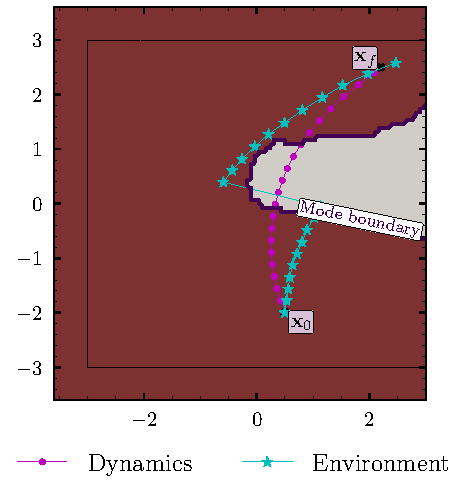
\includegraphics[width=\textwidth]{./images/traj-opt/mode-remaining/scenario_7_svgp_baseline_both_modes.pdf}
\subcaption{\acrshort{gp} dynamics model trained on state transitions sampled from \textbf{both} dynamics modes.}
\label{fig-traj-opt-over-gating-mask-svgp-all-baseline}
\end{minipage}
\begin{minipage}{0.49\textwidth}
\centering
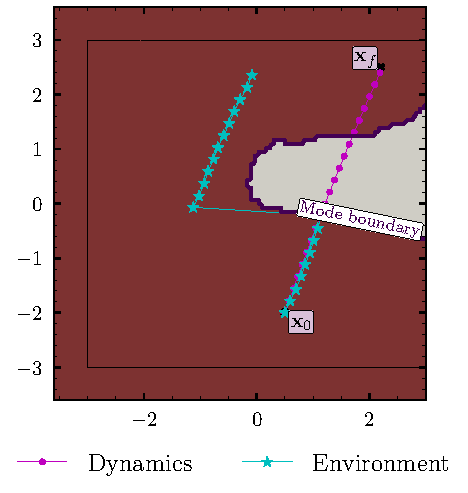
\includegraphics[width=\textwidth]{./images/traj-opt/mode-remaining/scenario_7_svgp_baseline_desired_mode.pdf}
\subcaption{\acrshort{gp} dynamics model trained on state transitions sampled from \textbf{only the desired} (operable) dynamics mode.}
\label{fig-traj-opt-over-gating-mask-svgp-desired-baseline}
\end{minipage}
\caption[Motivation for multimodal dynamical models]{
Trajectory optimisation results obtained using a \acrshort{gp} dynamics model trained on different data sets.
The optimised control trajectories are rolled out in the \acrshort{gp} dynamics model (magenta) and in the environment (cyan).
The state trajectories are overlayed on the gating mask, which indicates where each mode governs the dynamics.
White indicates the turbulent dynamics mode and red indicates the desired (operable) mode.}
\label{fig-traj-opt-over-gating-mask-svgp-baseline}
\end{figure}
In contrast to the previously presented  approaches, we are interested in learning representations
of multimodal dynamical systems.
\cref{fig-traj-opt-over-gating-mask-svgp-all-baseline}
demonstrates the shortcomings of learning a \acrshort{gp} dynamics model for the quadcopter navigation problem in the
illustrative example from \cref{illustrative_example}.
It shows the results of performing trajectory optimisation in a \acrshort{gp} dynamics model trained on state
transitions sampled from \textbf{both} dynamics modes.
The \acrshort{gp} has not been able to learn a representation of the dynamics which is true to the underlying system,
due to the discontinuities associated with the multimodal transition dynamics (changing lengthscales/noise variances etc).
The trajectory optimiser was able to find a trajectory from the start state \(\state_0\),
to the target state \(\targetState\) in the \acrshort{gp} dynamics (magenta).
However, as the \acrshort{gp} dynamics do not accurately represent the true underlying dynamics,
the state trajectory resulting from rolling out the optimised controls in the environment (cyan) does not match
the \acrshort{gp} dynamics trajectory (magenta).
This example motivates the need to correctly identify the underlying modes when learning representations of
multimodal dynamical systems for control.

\cref{fig-traj-opt-over-gating-mask-svgp-desired-baseline} shows results after training on state transitions from
only the desired, operable dynamics mode (red).
The learned dynamics model can accurately predict state transitions in the desired dynamics mode (red).
However, as this approach only considers the dynamics of the desired mode,
trajectories in the environment (cyan) deviate from those planned in the
learned dynamics model (magenta) when they pass through the turbulent mode.
This is problematic because the trajectory passes through the turbulent dynamics mode
(which may lead to catastrophic failure) and does not reach the target state \(\targetState\).
Without inferring information regarding how the system switches between its underlying dynamics modes, it is not
possible to encode mode remaining behaviour into control algorithms.
\begin{remark}
As the underlying dynamics modes and how the system switches between them,
are \textit{not fully known a priori}, partitioning the data set and learning the dynamics model in
\cref{fig-traj-opt-over-gating-mask-svgp-desired-baseline} is not possible in realistic scenarios.
\end{remark}


\begin{myquote}
Following standard methodologies, the trajectories in \cref{fig-traj-opt-over-gating-mask-svgp-baseline}
were found by minimising the expected cost
under the state distribution, resulting from cascading single-step predictions through the \acrshort{gp} dynamics model
using the moment matching approximation \citep{kussGaussian2006}.
A terminal state cost term favoured trajectories ending at the target state and
a quadratic integral control cost term regularised the controls to encode the notion of
"minimal effort" control.
\end{myquote}

Methods for learning probabilistic multimodal dynamics have been proposed.
\cite{moerlandLearning2017} use deep generative models, namely a conditional \acrfull{vae},
to learn multimodal transition dynamics for \acrshort{mbrl}.
\cite{kaiserBayesian2020} use the data association with \acrshort{gps} model;
a Bayesian model that learns independent dynamics modes whilst maintaining a
probabilistic belief over which mode is responsible for predicting at a given input location.
\cite{mckinnonLearning2017} also use an approach based on \acrshort{gps}, except that they use a
\acrfull{mogpe} method to learn the switching behaviour for robot dynamics online.

\textbf{Latent spaces for control}
It is worth noting that the introduction of \emph{latent variables} into probabilistic models
is a key component providing them with interesting and powerful capabilities for synergising model learning and control.
For example, \cite{hafnerLearning2019,rybkinModelBased2021} learn \emph{latent spaces} which provide
convenient spaces for control (or planning).
\cref{fig-traj-opt-over-gating-mask-svgp-desired-baseline} highlights the need for learning
informative latent variables representing how the system switches between the underlying dynamics modes.
Without such information, it is not possible to encode the notion of mode remaining/avoiding behaviour.
As such, this work is interested in learning \emph{latent spaces}
that are rich with information regarding how a system switches between its underlying dynamics modes.

\section{Uncertainty-based Exploration Strategies \label{sec-unc-exploration}}
\label{sec:org53b37ff}
\acrfull{rl} agents face a trade-off between \emph{exploration}, where they seek to explore the environment and improve
their models, and \emph{exploitation}, where they make decisions which are optimal for the data observed so far.
There are many approaches from the literature used to tackle the exploration-exploitation trade-off.
In \acrshort{mbrl}, the goal is often to reduce the real-world sample complexity at the cost of increased
model sample complexity.

There are two main uncertainties which are often modelled and used for exploration.
Value-based methods base their exploration on the uncertainty of the value function \(V\) at the current state \(\state_t\).
Actions with higher value estimates get higher probabilities of being selected based on
uncertainty estimates around the values \citep{moerlandEfficient2017,auerUsing2002}.
An alternative approach for \acrshort{mbrl} is to use state-based exploration.
This approach is state-specific, reward independent and usually seeks states with high \emph{epistemic uncertainty}.
This section recaps some relevant exploration strategies that fit into the general
\acrshort{mbrl} procedure shown in \cref{alg-mbrl-background}.

\textbf{Greedy exploitation}
One of the most commonly used exploration strategies is to select the controller that maximises
the expected performance under the learned dynamics model \(\dynamicsModel(f \mid \mathcal{D}_{0:i-1})\).
Note that \(i\) denotes the iteration/episode number of the \acrshort{mbrl} loop.
This greedy strategy is given by,
\begin{align} \label{eq-greedy-exploration}
\pi_i^{\text{greedy}} = \arg \max_{\pi \in \Pi} \E_{f \sim \dynamicsModel(f \mid \mathcal{D}_{0:i-1})} \left[ -J(f, \pi) \right].
\end{align}
Note that the negative sign is used because the objective \(J(f, \pi)\) is based on a cost function and not a reward
function.
This approach is used in \acrshort{pilco} \citep{deisenrothPILCO2011} and \acrshort{gp}-\acrshort{mpc} \citep{kamtheDataEfficient2018}
where the dynamics are represented using \acrshort{gps} and the moment matching approximation is used to cascade
single-step predictions.
\cite{parmasPIPPS2018} propose \acrshort{pipps},
a similar approach to \acrshort{pilco}, except that they use Monte Carlo methods
to propagate uncertainty forward in time, instead of using the moment matching approximation.
Similarly, \acrshort{pets} \citep{chuaDeep2018} uses this exploration strategy but represents the dynamics
using ensembles of probabilistic neural networks.
This strategy initially favours exploring regions of the environment where the learned dynamics
model is not confident, i.e. has high \emph{epistemic uncertainty}.
Once it has gathered knowledge of the environment and the model’s
epistemic uncertainty has been reduced, it favours maximising the objective function \(J(f, \pi)\).

\textbf{Thompson sampling}
An alternative and theoretically grounded strategy is Thompson sampling.
This approach samples a single model  \(f_i \sim \dynamicsModel(f \mid \mathcal{D}_{0:i})\) at every iteration \(i\)
and uses the sampled model to optimise the controller.
This is given by,
\begin{align} \label{eq-thompson-exploration}
\pi_i^{\text{thompson}} = \arg \max_{\pi \in \Pi} -J(f_i, \pi) \quad \text{s.t.} \quad f_i \sim \dynamicsModel(f \mid \mathcal{D}_{0:i}).
\end{align}

In general, it is intractable to sample from \(\dynamicsModel(f \mid \mathcal{D}_{0:i})\).
Note that after the sampling step this problem is equivalent to greedy exploitation.

Alternatively, some \acrshort{mbrl} algorithms, such as \cite{sekarPlanning2020}, adopt a two-phase exploration strategy.
The first phase is interested in exploring the environment and summarising this past experience in the form of a model.
The second phase then seeks to solve a downstream task, for which it is given a cost (reward) function.
This two-stage approach does not require an objective that changes its exploration-exploitation balance as
it gathers more knowledge of the environment.


\textbf{Active learning}
Active learning is a class of exploration algorithms which fit into the two-phase exploration approach.
The goal of information-theoretic active learning is to reduce the number of
possible hypotheses as fast as possible, e.g. minimise the uncertainty associated
with the parameters using Shannon's entropy \citep{coverElements2006},
\newcommand{\crv}{\ensuremath{X}}
\newcommand{\density}{\ensuremath{p(\crv)}}
\begin{myquote}
\textbf{Differential Entropy}
Let $\crv$ be a continuous random variable, with a probability density
$\density$,
whose support is a set $\mathcal{X}$.
The differential entropy $H[\crv]$ is then defined as,
\begin{align} \label{eq-differential-entropy}
H[\crv] = - \int_{\mathcal{X}} \density \text{log} \density \text{d} \crv.
\end{align}
\end{myquote}
In contrast to greedy exploitation, active learning does not seek to maximise a
black-box objective. Instead, it is only interested in exploration. There are many
approaches to active learning in the static setting, i.e. in systems where an arbitrary
state \(\state\) can be sampled. In contrast, dynamical systems must be steered to \(\state\)
through the unknown dynamics \(f\) through a sequence of controls \(\controlTraj\). Thus,
information gain along the trajectory must also be considered. As highlighted
by \cite{buisson-fenetActively2020}, information gain in dynamical systems is
fundamentally different to the static problem addressed by \cite{krauseNearOptimal2008}  and
\cite{houlsbyBayesian2011}.
The goal is to pick the most informative control trajectory
\(\controlTraj\) whilst observing \(\stateTraj\).

Recent work has addressed active learning in \acrshort{gp} dynamics models. \cite{schreiterSafe2015}
propose a greedy entropy-based strategy that considers the entropy of the
next state. \cite{buisson-fenetActively2020} also propose a greedy entropy-based strategy
except that they consider the entropy accumulated over a trajectory. In contrast,
\cite{caponeLocalized2020,yuActive2021} propose using the mutual information.
\begin{myquote}
\textbf{Mutual Information}
Given two sets of random variables, $\mathbf{X}$ and $\mathbf{F}$, with joint density $p(\mathbf{X}, \mathbf{F})$ the
mutual information \citep{coverElements2006} is given by,
\begin{align} \label{eq-mutual-information}
I[\mathbf{X};\mathbf{F}] = \int p(\mathbf{X},\mathbf{F}) \text{log}\frac{p(\mathbf{X},\mathbf{F})}{p(\mathbf{X})p(\mathbf{F})}
\text{d}\mathb{X} \text{d}\mathb{F},
\end{align}
and its well-known relationship to differential entropy $H[\cdot]$ is given by,
\begin{align} \label{eq-mutual-information-entropy}
I[\mathbf{X};\mathbf{F}] =  H[\mathbf{X}] - H[\mathbf{X} \mid \mathbf{F}].
\end{align}
\end{myquote}
\cite{caponeLocalized2020} find the most informative state as the one that minimises the
mutual information between it and a set of reference states (a discretisation of the
domain). They then find a set of controls to drive the system to this most informative state.
Given a fixed number of time steps, their method yields a better model
than the greedy entropy-based strategies.
\cite{yuActive2021}  propose an alternative
approach that leverages their \acrfull{gpssm} inference scheme to estimate the mutual
information between all the variables in time
\(I \left[\mathbf{y}_{1:t}, \hat{\mathbf{y}}_{t+1} ; \mathbf{f}_{1:t+1} \right]\).
Here \(\mathbf{y}_{1:t}\) denotes the set of observed outputs and \(\hat{\mathbf{y}}_{t+1}\) denotes
the output predicted by the \acrshort{gpssm}. This contrasts with other approaches, which
study the latest mutual information \(I[\hat{\mathbf{y}}_{t+1} ; \mathbf{f}_{t+1}]\).

\textbf{Myopic active learning}
In \acrshort{rl} and control it is standard to consider objectives over a potentially infinite horizon.
However, active learning objectives often myopically consider the information gain at the next query point only.
In contrast, it is possible to consider the information gain over a potentially infinite horizon, reliving this myopia.
The mutual information approaches in \cite{caponeLocalized2020,yuActive2021}
fall into this myopic category as they only maximise the information gain at the next
time step. In contrast, the entropy-based strategy in
\cite{buisson-fenetActively2020} considers the entropy over a horizon.

\chapter{Probabilistic Inference for Learning Multimodal Dynamical Systems \label{chap-dynamics}}
\label{sec:org4e986eb}
\epigraph{All models are wrong, but some are useful.}{\textit{George Box}}
\newcommand{\stateDomain}{\ensuremath{\mathcal{X}}}
%\renewcommand{\stateDomain}{\ensuremath{\mathcal{S}}}
\renewcommand{\controlDomain}{\ensuremath{\mathcal{U}}}
\renewcommand{\modeDomain}{\ensuremath{\mathcal{A}}}
%\renewcommand{\inputDomain}{\ensuremath{\mathcal{X}}}
\renewcommand{\inputDomain}{\ensuremath{\mathcal{Z}}}

%\renewcommand{\state}{\ensuremath{\mathbf{s}}}
\renewcommand{\state}{\ensuremath{\mathbf{x}}}

%\renewcommand{\nominalDynamics}{\ensuremath{\mathbf{n}}}
%\renewcommand{\unknownDynamics}{\ensuremath{\mathbf{f}}}
%\renewcommand{\nominalDynamicsK}{\ensuremath{\mode{\mathbf{n}}}}
%\renewcommand{\unknownDynamicsK}{\ensuremath{\mode{\mathbf{f}}}}

\renewcommand{\unknownDynamics}{\ensuremath{f}}
\renewcommand{\unknownDynamicsK}{\ensuremath{\mode{f}}}

\newcommand{\timeInd}{\ensuremath{t}}
\newcommand{\TimeInd}{\ensuremath{T}}
\newcommand{\inputDim}{\ensuremath{d}}
\newcommand{\InputDim}{\ensuremath{D}}
\newcommand{\tightBound}{\ensuremath{\mathcal{L}_{\text{tight}}}}
\newcommand{\furtherBound}{\ensuremath{\mathcal{L}_{\text{further}}}}
\newcommand{\furtherBoundTwo}{\ensuremath{\mathcal{L}_{\text{further}^2}}}
\renewcommand{\mode}[1]{\ensuremath{#1_{\modeInd}}}
\renewcommand{\modei}[2]{\ensuremath{#1_{#2}}}
%\renewcommand{\singleOutput}{\ensuremath{\Delta x_{\numData}}}
%\renewcommand{\allOutput}{\ensuremath{\Delta\mathbf{\state}}}
\newcommand{\singleModeVar}{\ensuremath{\singleData{\modeVar}}}
\newcommand{\allModeVar}{\ensuremath{\bm{\modeVar}}}
\newcommand{\singleModeVarK}{\ensuremath{\singleModeVar = \modeInd}}
\newcommand{\allModeVarK}{\ensuremath{\bm{\modeVar}_{\modeInd}}}
%\newcommand{\allModeVarK}{\ensuremath{\{\singleModeVarK\}_{\numData=1}^\NumData}}
\newcommand{\modeVarnk}{\ensuremath{\modeVar_{\numData,\modeInd}}}

% new
\renewcommand{\numData}{\ensuremath{n}}
\renewcommand{\NumData}{\ensuremath{N}}
\renewcommand{\singleOutput}{\ensuremath{y_{\numData}}}
\renewcommand{\singleInput}{\ensuremath{\mathbf{x}_{\numData}}}
\renewcommand{\allInput}{\ensuremath{\mathbf{X}}}
\renewcommand{\allOutput}{\ensuremath{\mathbf{y}}}
\renewcommand{\allOutput}{\ensuremath{\mathbf{y}}}
%\renewcommand{\allInputK}{\ensuremath{\{\singleInput : \singleModeVarK \}}}
%\renewcommand{\allOutputK}{\ensuremath{\{\singleOutput : \singleModeVarK\}}}
%\renewcommand{\allInputK}{\ensuremath{\allInput^{\modeInd}}}
%\renewcommand{\allOutputK}{\ensuremath{\allOutput^{\modeInd}}}
\renewcommand{\singleInputK}{\ensuremath{\mathbf{x}_{\numData, \modeInd}}}
\renewcommand{\allInputK}{\ensuremath{\mode{\allInput}}}
\renewcommand{\allOutputK}{\ensuremath{\mode{\allOutput}}}

%\renewcommand{\x}{\ensuremath{\mathbf{z}}}
%\renewcommand{\y}{\ensuremath{y}}
%\renewcommand{\singleInput}{\ensuremath{\mathbf{z}_{\numData}}}
%\renewcommand{\allInput}{\ensuremath{\mathbf{Z}}}
%\renewcommand{\singleInputK}{\ensuremath{\mathbf{z}_{\numData, \modeInd}}}
%\renewcommand{\allInputK}{\ensuremath{\mode{\allInput}}}

%\newcommand{\expertPrior}{\ensuremath{p\left(\mode{f}(\allInput) \right)}}
\newcommand{\expertPrior}{\ensuremath{p\left(\mode{f}(\allInputK) \right)}}
\newcommand{\expertsPrior}{\ensuremath{p\left(\LatentFunc(\allInput) \right)}}
\newcommand{\expertMeanFunc}{\ensuremath{\mode{\mu}}}
\newcommand{\expertCovFunc}{\ensuremath{\mode{k}}}
\newcommand{\expertLikelihood}{\ensuremath{p\left(\allOutput \mid \mode{f}(\allInput)\right)}}
\newcommand{\singleExpertLikelihood}{\ensuremath{p(\singleOutput \mid \mode{f}(\singleInput))}}
%\newcommand{\allExpertLikelihood}{\ensuremath{p(\allOutput \mid \mode{f}(\allInput))}}
%\newcommand{\allExpertLikelihood}{\ensuremath{p(\allOutputK \mid \mode{f}(\allInputK))}}
\newcommand{\allExpertLikelihood}{\ensuremath{p(\allOutputK \mid \mode{f}(\allInputK))}}
\newcommand{\expertPosterior}{\ensuremath{p\left(\allOutput \mid \allModeVarK, \allInput \right)}}
\newcommand{\singleExpertPosterior}{\ensuremath{p\left(\singleOutput \mid \singleModeVarK, \allInput \right)}}
% \newcommand{\expertPosterior}{\ensuremath{p\left(\allOutput \mid \allModeVarK \right)}}

\newcommand{\gatingPrior}{\ensuremath{p\left(\GatingFunc(\allInput ) \right)}}
\newcommand{\gatingMeanFunc}{\ensuremath{\mode{\hat{\mu}}}}
\newcommand{\gatingCovFunc}{\ensuremath{\mode{\hat{k}}}}
\newcommand{\singleGatingLikelihood}{\ensuremath{\Pr\left(\singleModeVarK \mid \GatingFunc(\singleInput) \right)}}
%\newcommand{\allGatingLikelihood}{\ensuremath{\Pr\left(\allModeVarK \mid \GatingFunc(\allInput) \right)}}
\newcommand{\allGatingLikelihood}{\ensuremath{p\left(\allModeVar \mid \GatingFunc(\allInput) \right)}}
\newcommand{\gatingLikelihood}{\ensuremath{P\left(\singleModeVar \mid \GatingFunc(\singleInput) \right)}}
%\newcommand{\gatingPosterior}{\ensuremath{\Pr\left( \singleModeVar \mid \singleInput \right)}}
\newcommand{\gatingPosterior}{\ensuremath{\Pr\left( \allModeVarK \mid \allInput \right)}}
\newcommand{\singleGatingPosterior}{\ensuremath{\Pr\left( \singleModeVarK \mid \singleInput, \gatingParams \right)}}
\newcommand{\evidence}{\ensuremath{p\left(\allOutput \mid \allInput \right)}}

\newcommand{\moeExpertPosterior}{\ensuremath{p\left(\singleOutput \mid \singleModeVarK, \singleInput, \expertParamsK \right)}}
\newcommand{\moeGatingPosterior}{\ensuremath{\Pr\left(\singleModeVarK \mid \singleInput, \gatingParams \right)}}
\newcommand{\moeEvidence}{\ensuremath{p\left(\allOutput \mid \allInput, \expertParams, \gatingParams \right)}}
\newcommand{\singleMoeEvidence}{\ensuremath{p\left(\singleOutput \mid \singleInput, \expertParams, \gatingParams \right)}}

\newcommand{\npmoeExpertPosterior}{\ensuremath{p\left(\allOutput \mid \allModeVar, \allInput, \expertParams \right)}}
\newcommand{\npmoeGatingPosterior}{\ensuremath{p\left(\allModeVar \mid \allInput, \gatingParams \right)}}

\newcommand{\moeLikelihood}{\ensuremath{p\left(\allOutput \mid \LatentFunc(\allInput), \GatingFunc (\allInput) \right)}}
\newcommand{\singleMoeLikelihood}{\ensuremath{p\left(\singleOutput \mid \mode{\latentFunc}(\allInput), \GatingFunc (\allInput) \right)}}
%\renewcommand{\expertKernelnn}{\ensuremath{k_{\singleInput\singleInput}}}
%\renewcommand{\expertKernelnM}{\ensuremath{\mathbf{k}_{\singleInput \expertInducingInput}}}
%\renewcommand{\expertKernelMM}{\ensuremath{\mathbf{K}_{\expertInducingInput\expertInducingInput}}}
%\renewcommand{\expertKernelMn}{\ensuremath{\mathbf{k}_{\expertInducingInput \singleInput}}}
\renewcommand{\expertKernelnn}{\ensuremath{k_{\modeInd \numData \numData}}}
\renewcommand{\expertKernelNN}{\ensuremath{\mathbf{K}_{\modeInd \NumData \NumData}}}
\renewcommand{\expertKernelnM}{\ensuremath{\mathbf{k}_{\modeInd \numData \NumInducing}}}
\renewcommand{\expertKernelNM}{\ensuremath{\mathbf{K}_{\modeInd \NumData \NumInducing}}}
\renewcommand{\expertKernelMM}{\ensuremath{\mathbf{K}_{\modeInd \NumInducing \NumInducing}}}
\renewcommand{\expertKernelMn}{\ensuremath{\mathbf{k}_{\modeInd \NumInducing \numData}}}
\renewcommand{\expertKernelMN}{\ensuremath{\mathbf{K}_{\modeInd \NumInducing \NumData}}}
\renewcommand{\expertKernelsM}{\ensuremath{\mathbf{k}_{\modeInd * \NumInducing}}}
\renewcommand{\expertKernelss}{\ensuremath{k_{\modeInd **}}}
\renewcommand{\expertKernelSM}{\ensuremath{\mathbf{K}_{\modeInd * \NumInducing}}}
\renewcommand{\expertKernelSS}{\ensuremath{\mathbf{K}_{\modeInd **}}}

%\renewcommand{\gatingKernelnn}{\ensuremath{\hat{k}_{\singleInput\singleInput}}}
%\renewcommand{\gatingKernelnM}{\ensuremath{\hat{\mathbf{k}}_{\singleInput \gatingInducingInput}}}
%\renewcommand{\gatingKernelMM}{\ensuremath{\hat{\mathbf{K}}_{\gatingInducingInput\gatingInducingInput}}}
%\renewcommand{\gatingKernelMn}{\ensuremath{\hat{\mathbf{k}}_{\gatingInducingInput \singleInput}}}
\renewcommand{\gatingKernelnn}{\ensuremath{\hat{k}_{\modeInd \numData \numData}}}
\renewcommand{\gatingKernelNN}{\ensuremath{\hat{\mathbf{K}}_{\modeInd \NumData \NumData}}}
\renewcommand{\gatingKernelnM}{\ensuremath{\hat{\mathbf{k}}_{\modeInd \numData \NumInducing}}}
\renewcommand{\gatingKernelNM}{\ensuremath{\hat{\mathbf{K}}_{\modeInd \NumData \NumInducing}}}
\renewcommand{\gatingKernelMM}{\ensuremath{\hat{\mathbf{K}}_{\modeInd \NumInducing \NumInducing}}}
\renewcommand{\gatingKernelMn}{\ensuremath{\hat{\mathbf{k}}_{\modeInd \NumInducing \numData}}}
\renewcommand{\gatingKernelss}{\ensuremath{\hat{k}_{\modeInd **}}}
\renewcommand{\gatingKernelsM}{\ensuremath{\hat{\mathbf{k}}_{\modeInd * \NumInducing}}}
\renewcommand{\gatingKernelMs}{\ensuremath{\hat{\mathbf{k}}_{\modeInd \NumInducing *}}}
\renewcommand{\gatingKernelSM}{\ensuremath{\hat{\mathbf{K}}_{\modeInd * \NumInducing}}}
\renewcommand{\gatingKernelMS}{\ensuremath{\hat{\mathbf{K}}_{\modeInd \NumInducing *}}}
\renewcommand{\gatingKernelSS}{\ensuremath{\hat{\mathbf{K}}_{\modeInd **}}}

\renewcommand{\expertA}{\ensuremath{\mode{\mathbf{A}}}}
\renewcommand{\gatingA}{\ensuremath{\mode{\hat{\mathbf{A}}}}}
\renewcommand{\input}{\ensuremath{\hat{\state}}}
\renewcommand{\output}{\ensuremath{\Delta \state}}

\newcommand{\kernel}{\ensuremath{k}}
\newcommand{\expertKernel}{\ensuremath{\mode{\kernel}}}
\newcommand{\gatingKernel}{\ensuremath{\mode{\hat{\kernel}}}}

\newcommand{\numInducing}{\ensuremath{m}}
\newcommand{\NumInducing}{\ensuremath{\MakeUppercase{\numInducing}}}
%\newcommand{\inducingInput}{\ensuremath{\mathbf{Z}}}
\newcommand{\inducingInput}{\ensuremath{\bm{\zeta}}}
\newcommand{\inducingOutput}{\ensuremath{\mathbf{u}}}

%\newcommand{\expertInducingInput}{\ensuremath{\mode{\inducingInput}}}
%\newcommand{\expertsInducingInput}{\ensuremath{\inducingInput}}}
\newcommand{\expertInducingInput}{\ensuremath{\mode{\bm{\zeta}}}}
\newcommand{\expertsInducingInput}{\ensuremath{\bm{\zeta}}}
%\newcommand{\expertInducingOutput}{\ensuremath{\mode{\inducingOutput}}}
%\newcommand{\expertsInducingOutput}{\ensuremath{\MakeUppercase{\inducingOutput}}}
%\newcommand{\expertInducingOutput}{\ensuremath{\mode{\hat{\mathbf{\latentFunc}}}}}
%\newcommand{\expertsInducingOutput}{\ensuremath{\hat{\MakeUppercase{\mathbf{\latentFunc}}}}}
%\newcommand{\expertInducingOutput}{\ensuremath{\mode{\tilde{\mathbf{\latentFunc}}}}}
%\newcommand{\expertsInducingOutput}{\ensuremath{\tilde{\MakeUppercase{\mathbf{\latentFunc}}}}}
\newcommand{\expertInducingOutput}{\ensuremath{\mode{\latentFunc}(\expertInducingInput)}}
\newcommand{\expertsInducingOutput}{\ensuremath{\mathbf{\latentFunc}(\expertsInducingInput)}}

%\newcommand{\gatingInducingInput}{\ensuremath{\hat{\inducingInput}}}
\newcommand{\gatingInducingInput}{\ensuremath{\bm{\xi}}}
%\newcommand{\gatingInducingOutput}{\ensuremath{\mode{\hat{\inducingOutput}}}}
%\newcommand{\gatingsInducingOutput}{\ensuremath{\hat{\MakeUppercase{\inducingOutput}}}}
%\newcommand{\gatingInducingOutput}{\ensuremath{\mode{\hat{\mathbf{\gatingFunc}}}}}
%\newcommand{\gatingsInducingOutput}{\ensuremath{\hat{\MakeUppercase{\mathbf{\gatingFunc}}}}}
%\newcommand{\gatingInducingOutput}{\ensuremath{\mode{\tilde{\mathbf{\gatingFunc}}}}}
%\newcommand{\gatingsInducingOutput}{\ensuremath{\tilde{\MakeUppercase{\mathbf{\gatingFunc}}}}}
\newcommand{\gatingInducingOutput}{\ensuremath{\mode{\gatingFunc}(\gatingInducingInput)}}
\newcommand{\gatingsInducingOutput}{\ensuremath{\mathbf{\gatingFunc}(\gatingInducingInput)}}

%\newcommand{\expertInducingPrior}{\ensuremath{p(\mode{\latentFunc}(\expertInducingInput))}}
%\newcommand{\expertInducingPrior}{\ensuremath{p(\expertInducingOutput \mid \expertInducingInput)}}
%\newcommand{\expertsInducingPrior}{\ensuremath{p(\expertsInducingOutput \mid \expertsInducingInput)}}
\newcommand{\expertInducingPrior}{\ensuremath{p(\expertInducingOutput)}}
\newcommand{\expertsInducingPrior}{\ensuremath{p(\expertsInducingOutput)}}
%\newcommand{\expertInducingVariational}{\ensuremath{q(\mode{\latentFunc}(\expertInducingInput))}}
\newcommand{\expertInducingVariational}{\ensuremath{q(\expertInducingOutput)}}
\newcommand{\expertsInducingVariational}{\ensuremath{q(\expertsInducingOutput)}}
\newcommand{\expertVariational}{\ensuremath{q(\mode{\latentFunc}(\singleInput))}}
\newcommand{\expertsVariational}{\ensuremath{q(\LatentFunc(\singleInput))}}
%\newcommand{\singleExpertGivenInducing}{\ensuremath{p(\singleOutput \mid \mode{\latentFunc}(\expertInducingInput))}}
\newcommand{\singleExpertGivenInducing}{\ensuremath{p(\singleOutput \mid \expertInducingOutput)}}
\newcommand{\allExpertGivenInducing}{\ensuremath{p(\allOutput \mid \expertInducingOutput)}}
%\newcommand{\singleLatentExpertGivenInducing}{\ensuremath{p(\mode{\latentFunc}(\singleInput) \mid \mode{\latentFunc}(\expertInducingInput))}}
\newcommand{\singleLatentExpertGivenInducing}{\ensuremath{p(\mode{\latentFunc}(\singleInput) \mid \expertInducingOutput)}}
\newcommand{\allLatentExpertGivenInducing}{\ensuremath{p(\mode{\latentFunc}(\allInput) \mid \expertInducingOutput)}}


%\newcommand{\gatingInducingPrior}{\ensuremath{p(\GatingFunc(\gatingInducingInput))}}
%\newcommand{\gatingInducingPrior}{\ensuremath{p(\gatingInducingOutput \mid \gatingInducingInput)}}
%\newcommand{\gatingsInducingPrior}{\ensuremath{p(\gatingsInducingOutput \mid \gatingInducingInput)}}
\newcommand{\gatingInducingPrior}{\ensuremath{p(\gatingInducingOutput)}}
\newcommand{\gatingsInducingPrior}{\ensuremath{p(\gatingsInducingOutput)}}
%\newcommand{\gatingInducingVariational}{\ensuremath{q(\GatingFunc(\gatingInducingInput))}}
\newcommand{\gatingInducingVariational}{\ensuremath{q(\gatingInducingOutput)}}
\newcommand{\gatingsInducingVariational}{\ensuremath{q(\gatingsInducingOutput)}}
\newcommand{\gatingsVariational}{\ensuremath{q(\GatingFunc(\singleInput))}}
\newcommand{\singleGatingGivenInducing}{\ensuremath{\Pr(\singleModeVarK \mid \gatingsInducingOutput)}}
\newcommand{\allGatingGivenInducing}{\ensuremath{\Pr(\allModeVarK \mid \gatingInducingOutput)}}
\newcommand{\allGatingsGivenInducing}{\ensuremath{\Pr(\allModeVarK \mid \gatingsInducingOutput)}}
\newcommand{\singleLatentGatingsGivenInducing}{\ensuremath{p(\GatingFunc(\singleInput) \mid \gatingsInducingOutput)}}
\newcommand{\allLatentGatingsGivenInducing}{\ensuremath{p(\GatingFunc(\allInput) \mid \gatingsInducingOutput)}}
\newcommand{\singleLatentGatingGivenInducing}{\ensuremath{p(\mode{\gatingFunc}(\singleInput) \mid \gatingInducingOutput)}}

\newcommand{\expertKL}{\ensuremath{\text{KL}\left( \expertInducingVariational \mid\mid \expertInducingPrior \right)}}
\newcommand{\expertsKL}{\ensuremath{\sum_{\modeInd=1}^\ModeInd\text{KL}\left( \expertInducingVariational \mid\mid \expertInducingPrior \right)}}
\newcommand{\gatingKL}{\ensuremath{\text{KL}\left( \gatingInducingVariational \mid\mid \gatingInducingPrior \right)}}
\newcommand{\gatingsKL}{\ensuremath{\sum_{\modeInd=1}^\ModeInd \text{KL}\left( \gatingInducingVariational \mid\mid \gatingInducingPrior \right)}}
This chapter is concerned with \emph{learning} representations of multimodal dynamical systems for model-based control.
It is interested in systems where both the underlying
dynamics modes and how the system switches between them, are \emph{not fully known a priori}.
This chapter assumes access to a data set of state transitions \(\dataset\),
previously sampled from the system at a constant frequency, i.e. with a fixed time-step.

Following the motivation in \cref{to_motivation}, this chapter
seeks to identify the underlying dynamics modes correctly whilst inferring
latent structure that can be exploited for control.
The main goals of this chapter can be summarised as follows,
\begin{enumerate}
\item accurately \emph{identify} the true underlying dynamics modes,
\item learn \emph{latent spaces} for planning/control.
\end{enumerate}
The probabilistic model constructed in this chapter
resembles a \acrfull{mogpe} with a \acrshort{gp}-based gating network and  is named \acrfull{mosvgpe}.
Following other \acrshort{mogpe} methods, it is evaluated on the motorcycle data set \citep{Silverman1985}.
It is then tested on a real-world quadcopter data set representing the illustrative
example detailed in \cref{illustrative_example}.
\section{Problem Statement}
\label{sec:org2122f14}
This work considers learning representations of \emph{unknown} or \emph{partially unknown}, stochastic, multimodal,
nonlinear dynamical systems.
That is, it seeks to learn a representation of the dynamics from the problem statement in \cref{problem-statement-main}.
This chapter considers single-step dynamics models with the delta state formulation
that regularises the predictive distribution.
The dynamics are given by,
%\begin{align} \label{eq-multimodal-dynamics-disc}
%\Delta \state_{\timeInd+1}
%&= \unknownDynamics(\state_{t}, \control_{t}; \Delta t = t_*) + \bm\epsilon & \nonumber \\
%&= \unknownDynamicsK (\state_{\timeInd}, \control_{\timeInd} ; \Delta t = t_*) + \mode{\bm\epsilon}
%&\text{if} \quad \modeVar(\state_{\timeInd}) = \modeInd
%\end{align}
\begin{subequations} \label{eq-multimodal-dynamics-disc}
\begin{align}
\Delta \state_{\timeInd+1} &= \dynamicsFunc(\state_\timeInd, \control_\timeInd) + \bm\epsilon \\
&= \mode{\dynamicsFunc}(\state_\timeInd, \control_\timeInd) + \mode{\bm\epsilon}
\quad \text{if} \quad \modeVar(\state_{\timeInd})=\modeInd \quad \forall \modeInd \in \{1,\ldots \ModeInd \} \nonumber \\
\mode{\bm\epsilon} &\sim \mathcal{N}(\mathbf{0}, \Sigma_{\mode{\bm\epsilon}}),
\end{align}
\end{subequations}
with continuous states \(\state_t \in \stateDomain \subseteq \R^\StateDim\), continuous controls
\(\control_t \in \controlDomain \subseteq \R^\ControlDim\) and time index \(t\).
The state difference between time \(\timeInd\) and \(\timeInd+1\) is denoted
\(\Delta \state_{\timeInd+1} = \state_{\timeInd+1} - \state_{\timeInd}\).
At any given time step \(t\), one of the \(\ModeInd\) dynamics modes
\(\{\unknownDynamicsK : \mode{\stateDomain} \times \controlDomain \rightarrow \stateDomain \}_{\modeInd=1}^\ModeInd\)
and associated noise models
\(\mode{\bm\epsilon} &\sim \mathcal{N}\left(\mathbf{0}, \bm\Sigma_{\mode{\bm\epsilon}} \right)\),
are selected by a discrete mode indicator variable
\(\alpha_{\timeInd} \in \modeDomain = \{1,\ldots,\ModeInd\}\).
This work assumes that the discrete mode indicator variable depends on the state \(\state\) such that it is governed by
a discrete mode indicator function \(\alpha : \stateDomain \rightarrow \modeDomain\).


This chapter assumes access to historical data comprising state transitions from \(\NumEpisodes\) trajectories
of length \(T\), sampled  with a  fixed  time step \(\Delta t=t_{*}\).
The data set has \({N=ET}\) elements
and we abuse notation by appending the independent trajectories along
time to get the data set
\(\mathcal{D}=\{(\state_{\timeInd},\control_{\timeInd}),\Delta \state_{t+1}\}^{\NumData-1}_{\timeInd=0}\).

To ease notation, our modelling only considers a single output dimension.
The extension to multiple output dimensions follows from standard \acrshort{gp} methodologies and is detailed where necessary.
To further ease notation, the state-control input domain is denoted
\(\inputDomain = \stateDomain \times \controlDomain \subseteq \R^{\InputDim}\)
and a single state-control input is denoted
\(\singleInput = (\state_{\timeInd},\control_{\timeInd})\).
Given this formulation, this chapter aims to learn the mapping \(\unknownDynamics\),
which switches between \(\ModeInd\) different functions \(\mode{\latentFunc}\).
This can be cast as a regression problem,
\begin{align} \label{eq-multimodal-dynamics-disc-regression}
\underbrace{\Delta \state_{t+1}}_{\text{\singleOutput}}
= \underbrace{\unknownDynamicsK(\state_{t}, \control_{t})}_{\text{\mode{\latentFunc} (\singleInput)}}
+ \mode{\epsilon}
\quad \text{if} \quad \modeVarK,
\end{align}
where both the latent dynamics functions \(\{\unknownDynamicsK\}_{\modeInd=1}^{\ModeInd}\)
and how the system switches between them
\(\modeVar\), must be inferred from observations.
A single observation is denoted as \((\singleInput, \singleOutput) = ((\state_{t},\control_{t}), \Delta \state_{t+1})\).
The set of all inputs is denoted as \(\allInput \in \R^{\NumData \times \InputDim\)
and the set of all outputs as \(\allOutput \in \R^{\NumData \times 1}\).
With this notation, the regression problem can be written as,
\begin{align} \label{eq-multimodal-dynamics-disc-regression-simple}
\singleOutput
= \mode{\latentFunc}(\singleInput) + \mode{\epsilon}
\quad \text{if} \quad \modeVarK.
\end{align}

\section{Preliminaries}
\label{sec:orgaa3100e}
\acrfull{gps} are the state-of-the-art approach for Bayesian nonparametric regression
and they provide a powerful mechanism for encoding expert domain knowledge.
They are flexible enough to model arbitrary smooth functions with the simplicity of only requiring
inference over a small number of interpretable parameters, such as
lengthscales and the contributions of signal and noise variance in the data.
These properties are induced by the \emph{covariance function}, which models the covariance between observations.
As such, \acrshort{mogpe} methods are a promising direction for modelling multimodal dynamical systems.
This section recaps the \acrshort{mogpe} concepts that this chapter builds upon.
\newline

\textbf{Mixture Models}
Mixture models are a natural choice for modelling multimodal systems.
Given an input \(\singleInput\) and an output \(\singleOutput\), mixture models
model a mixture of distributions over the output,
\begin{equation} \label{eq-mixture-model}
\singleMoeEvidence = \sum_{\modeInd=1}^\ModeInd
\underbrace{\Pr(\singleModeVarK \mid \gatingParams)}_{\text{mixing probability}}
\underbrace{p(\singleOutput \mid \modeVarK, \singleInput, \expertParamsK)}_{\text{component } k}.
\end{equation}
where \(\gatingParams\) and \(\expertParams\) represent model parameters
and \(\singleModeVar\) is a discrete indicator variable assigning observations to components.
The predictive distribution \(\singleMoeEvidence\) consists of
\(K\) mixture components \({p(\singleOutput \mid \modeVarK, \singleInput, \expertParamsK)}\) that are weighted according to
their mixing probabilities \(\Pr(\modeVarK \mid \gatingParams)\).
\newline

\textbf{Mixture of Experts} The \acrfull{moe} model \citep{jacobsAdaptive1991} is
an extension where the mixing probabilities
depend on the input variable \(\moeGatingPosterior\), and are
collectively referred to as the \emph{gating network}.
The individual component densities \(\moeExpertPosterior\) are then referred to as \emph{experts},
as at different regions in the input space, different components are responsible for predicting.
Given \(\ModeInd\) experts \(\moeExpertPosterior\), each with parameters \(\expertParamsK\),
the \acrshort{moe} marginal likelihood is given by,
\begin{align} \label{eq-mixture-marginal-likelihood}
\moeEvidence = \prod_{\numData=1}^\NumData \sum_{\modeInd=1}^{\ModeInd}
\underbrace{\moeGatingPosterior}_{\text{gating network}}
\underbrace{\moeExpertPosterior}_{\text{expert } k},
\end{align}
where \(\singleModeVar\) is the expert indicator variable assigning observations to experts.
The probability mass function over the expert indicator variable is referred to as the gating network and
indicates which expert governs the model at a given input location.
See \cite{yukselTwenty2012} for a survey of \acrshort{moe} methods.
Note the correspondence between the expert indicator variable \(\singleModeVar\)
and the mode indicator variable from \cref{eq-multimodal-dynamics-disc}.
\newline
\textbf{Nonparametric Mixtures of Experts}
Modelling the experts as \acrshort{gps} gives rise to a class of powerful models known as \acrfull{mogpe}.
They can model multimodal distributions as they model a mixture of distributions
over the outputs, usually a Gaussian mixture in the regression setting \citep{trespMixtures2000a,rasmussenInfinite2001}.
They can model non-stationary functions as
each expert learns separate hyperparameters (lengthscales, noise variances etc).
Many \acrshort{mogpe} methods have been proposed, and in general, they differ in
the formulation of their gating network and their approximate inference algorithms.

\begin{figure}[t]
  \centering
    \begin{minipage}[r]{0.49\textwidth}
%   \resizebox{0.8\columnwidth}{!}{
    \begin{tikzpicture}[
      pre/.style={<-,shorten <=0.4pt,>=stealth',semithick},
      post/.style={->,shorten >=0.4pt,>=stealth',semithick}
      ]
      \node[const] (x) {$\singleInputK$};

      \node[latent, left=of x, yshift=-1.4cm] (f) {$\mode{\latentFunc}(\allInputK)$};

      \node[const, left=of f, xshift=0.4cm] (thetak) {$\expertParamsK$};

      \node[latent, below=of x, xshift=0.0cm] (a) {$\modeVarnk$};

      \node[const, right=of a, xshift=-0.4cm] (phik) {$\gatingParams$};

      \node[obs, below=of f, yshift=0.4cm] (y) {$\allOutputK$};

      \node[const, left=of y] (sigmak) {$\noiseVarK$};

      %\node[obs, right=of sigmak] (y) {$\Delta\mathbf{x}_{t}$};

      \draw[post] (a)--(y);
      \draw[post] (x)-|(f);
      %\draw[post] (f)--(yk);
      %\draw[post] (f)--(yk);
      %\draw[post] (yk)--(y);
      %\draw[post] (h)--(a);
      \draw[post] (x)--(a);
      \draw[post] (thetak)--(f);
      \draw[post] (phik)--(a);
      %\draw[post] (sigmak)|-(yk);
      \draw[post] (sigmak)|-(y);
      \draw[post] (f)--(y);

      \plate {} {(x) (yk) (a)} {$\NumData_{\modeInd}$};
      %\plate {} {(zk) (uk) (f) (sigmak) (thetak) (yk)} {$K$};
      %\plate {} {(f) (sigmak) (thetak)} {$\ModeInd$};
      \plate {} {(x) (y) (f) (sigmak) (thetak) (a)} {$\ModeInd$};
    \end{tikzpicture}
    %}
    \subcaption{}
\label{fig-graphical-model-npmoe}
\end{minipage}
    \begin{minipage}[r]{0.49\textwidth}
%   \resizebox{0.8\columnwidth}{!}{
    \begin{tikzpicture}[
      pre/.style={<-,shorten <=0.4pt,>=stealth',semithick},
      post/.style={->,shorten >=0.4pt,>=stealth',semithick}
      ]
      \node[const] (x) {$\singleInputK$};

      \node[latent, left=of x, yshift=-1.4cm] (f) {$\mode{\latentFunc}(\allInputK)$};
      \node[const, left=of f, xshift=0.4cm] (thetak) {$\expertParamsK$};

      \node[latent, below=of x, xshift=0.0cm] (a) {$\modeVarnk$};
      \node[latent, right=of a, yshift=0.0cm] (h) {$\mode{\gatingFunc}(\allInput)$};
      \node[const, right=of h, xshift=-0.4cm] (phik) {$\gatingParamsK$};

      \node[obs, below=of f, yshift=0.4cm] (y) {$\allOutputK$};
      \node[const, left=of y] (sigmak) {$\noiseVarK$};

      \draw[post] (a)--(y);
      \draw[post] (x)-|(f);
      \draw[post] (x)-|(h);
      \draw[post] (h)--(a);
      \draw[post] (thetak)--(f);
      \draw[post] (phik)--(h);
      %\draw[post] (sigmak)|-(yk);
      \draw[post] (sigmak)|-(y);
      \draw[post] (f)--(y);

      \plate {} {(x) (yk) (a)} {$\NumData_{\modeInd}$};
      %\plate {} {(zk) (uk) (f) (sigmak) (thetak) (yk)} {$K$};
      %\plate {} {(f) (sigmak) (thetak)} {$\ModeInd$};
      \plate {} {(h) (phik)} {$\ModeInd$};
      \plate {} {(x) (y) (f) (sigmak) (thetak)  (a)} {$\ModeInd$};
    \end{tikzpicture}
    %}
    \subcaption{}
\label{fig-graphical-model-gp-gating-network}
\end{minipage}
  %\caption{Graphical model where the output $\singleOutput$}
  \caption[Graphical models of nonparametric mixtures of experts]{
  Graphical models where the outputs $\allOutput = \{\allOutputK\}_{\modeInd=1}^{\ModeInd}$
are generated by mapping the inputs $\allInput = \{\allInputK\}_{\modeInd=1}^{\ModeInd}$ through the latent processes.
  An input assigned to expert $\modeInd$ is denoted $\singleInputK$
  and the sets of all $\NumData_{\modeInd}$ inputs and outputs assigned to expert $\modeInd$ are denoted
  $\allInputK$ and $\allOutputK$ respectively.
The experts are shown on the left of each model and the gating network on the right.
The generative processes involve evaluating the gating network
and sampling an expert mode indicator variable $\singleModeVar$.
The indicated mode's latent function $\mode{f}$ and noise model $\mathcal{N}(0, \noiseVarK)$ are
then evaluated to generate the output $\singleOutput$.
  (\subref{fig-graphical-model-npmoe}) shows
   the Mixture of Gaussian Process Experts model first presented in
  \cite{rasmussenInfinite2001} but without the Dirichlet process prior on the gating network.
  This represents the basic conditional model, not the full generative model over both the inputs and outputs as
  presented in \cite{NIPS2005_f499d34b}.
  (\subref{fig-graphical-model-gp-gating-network}) shows our model with a \acrshort{gp}-based gating network
which involves evaluating $\ModeInd$ latent gating functions $\GatingFunc$
and normalising their output to obtain the mixing probabilities $\singleGatingLikelihood$.
The mode indicator variable $\singleModeVar$ is then sampled from the Categorical distribution
governed by these probabilities.}
\label{fig-graphical-model-comparison}
\end{figure}
\newline

\cite{rasmussenInfinite2001} highlighted that the traditional \acrshort{moe} marginal likelihood does not apply when the
experts are nonparametric.
This is because the model assumes that the observations are i.i.d. given the model parameters,
which is contrary to \acrshort{gp} models, which model the dependencies in the joint distribution, given the
hyperparameters.
\cite{rasmussenInfinite2001} point out that there is a joint distribution corresponding to every possible
combination of assignments (of observations to experts).
The marginal likelihood is then a sum over exponentially many (\(\ModeInd^{\NumData}\)) sets of assignments,
\small
\begin{align}  \label{eq-np-moe-marginal-likelihood-assign}
\moeEvidence &= \sum_{\allModeVar} \npmoeGatingPosterior \npmoeExpertPosterior  \nonumber \\
&= \sum_{\allModeVar} \npmoeGatingPosterior
\left[ \prod_{\modeInd=1}^\ModeInd p\left(\allOutputK \mid \allInputK, \expertParamsK \right) \right],
\end{align}
\normalsize
where \(\allModeVar = \{\modeVar_1, \ldots, \modeVar_\NumData \}\) represents a set of assignments for all observations.
\cref{fig-graphical-model-npmoe} shows its graphical model representation.
Note that \(\allInputK = \{\singleInput : \singleModeVarK \}_{\numData=1}^{\NumData_{\modeInd}}\) and
\(\allOutputK = \{\singleOutput : \singleModeVarK \}_{\numData=1}^{\NumData_{\modeInd}}\)
represent the \(\NumData_{\modeInd}\) inputs and outputs assigned to the \(\modeInd^{\text{th}}\)
expert respectively.
This distribution factors into the product over experts, where each expert models the joint Gaussian distribution
over the observations assigned to it.
Assuming a mixture of Gaussian process regression models,
the marginal likelihood in \cref{eq-np-moe-marginal-likelihood-assign}
can be expanded to show each of the experts' latent variables,
\begin{align} \label{eq-np-moe-marginal-likelihood}
%\moeEvidence
\evidence
%&= \sum_{\allModeVar} \npmoeGatingPosterior \npmoeExpertPosterior  \\
%&= \sum_{\allModeVar} \npmoeGatingPosterior
%\left[ \prod_{\modeInd=1}^\ModeInd p\left(\allOutputK \mid \allInputK, \expertParamsK \right) \right]   \\
&= \sum_{\allModeVar} \npmoeGatingPosterior
\left[ \prod_{\modeInd=1}^\ModeInd
\E_{\expertPrior} \left[
\prod_{\numData=1}^{\NumData_{\modeInd}}
p\left(\singleOutput \mid \mode{\latentFunc}(\singleInput) \right)
\right] \right],
\end{align}
where each expert follows the standard Gaussian likelihood model,
\begin{align} \label{eq-expert-likelihood}
\singleOutput &= \mode{f}(\singleInput) + \epsilon_{k}, \quad \epsilon_{k} \sim \mathcal{N}(0, \mode{\noiseVar}^2), \\
\singleExpertLikelihood &= \mathcal{N}\left( \singleOutput \mid \mode{f}(\singleInput), \mode{\noiseVar}^2 \right),
%\singleOutput \mid \modeVar, \mode{\latentFunc}(\singleInput) &\sim \mathcal{N}\left( \mode{f}(\singleInput), \mode{\noiseVar}^2 \right),
\end{align}
with \(\mode{f}\) and \(\mode{\noiseVar}^2\) representing the latent function and the noise variance associated
with the \(\modeInd\)\textsuperscript{\text{th}} expert.
Note that for notational conciseness the dependency on \(\modeVarK\) is dropped from
\(\singleExpertLikelihood\) as it is implied by the mode indexing \(\mode{\latentFunc}\).
The dependence on \(\gatingParams\) and \(\expertParams\) is also dropped from here on in.
Independent \acrshort{gp} priors are placed on each of the expert's latent functions,
\begin{align} \label{eq-single-expert-prior}
%\expertPrior &= \mathcal{N}\left( \mode{f}(\allInput) \mid \expertMeanFunc(\allInput), \expertCovFunc(\allInput, \allInput) \right) \\
%\mode{\latentFunc}(\allInput) &\sim \mathcal{N}\left( \expertMeanFunc(\allInput), \expertCovFunc(\allInput, \allInput) \right) \\
\mode{\latentFunc}(\allInputK) &\sim \mathcal{N}\left( \expertMeanFunc(\allInputK), \expertCovFunc(\allInputK, \allInputK) \right)
\end{align}
where \(\expertMeanFunc(\cdot)\) and \(\expertCovFunc(\cdot, \cdot)\) represent the mean and
covariance functions associated with the \(\modeInd^{\text{th}}\) expert respectively.
This leads to each expert resembling a standard \acrshort{gp} regression model with a Gaussian likelihood.
For notational conciseness the dependence on the inputs \(\allInputK\) and hyperparameters \(\expertParamsK\)
is dropped for each \acrshort{gp} prior,
i.e. \(\expertPrior = p\left( \mode{f}(\allInputK) \mid \allInputK, \expertParamsK \right)\).

\section{Identifiable Mixtures of Gaussian Process Experts}
\label{sec:org24bdf87}
Motivated by improving identifiability and learning latent spaces for control,
this work adopts a \acrshort{gp}-based gating network resembling a \acrshort{gp} classification model,
similar to that used in the original \acrshort{mogpe} model \citep{trespMixtures2000a}.
The \acrshort{gp}-based gating network can be used to constrain the set of
admissible functions through the placement of informative \acrshort{gp} priors on the gating functions.
Further to this, in \cref{chap-traj-opt-control}, the geometry of the \acrshort{gp}-based gating network is
used to encode mode remaining behaviour into control strategies.
\cref{chap-active-learning} then leverages the power of the \acrshort{gp}-based gating network to construct an
explorative trajectory optimisation algorithm that can consider the information gain over trajectories,
as opposed to just at the next state.

The marginal likelihood is given by,
\begin{align} \label{eq-marginal-likelihood-assign}
\evidence &=
\sum_{\allModeVar}
\underbrace{\E_{\gatingPrior} \left[
%\frac{1}{Z}
\prod_{\numData=1}^{\NumData}
\gatingLikelihood
% p(\modeVarn \mid \GatingFunc(\singleInput))
 \right]}_{\text{GP gating network}}
  \underbrace{\prod_{\modeInd=1}^\ModeInd p\left(\{\singleOutput : \singleModeVarK \} \mid \{\singleInput : \singleModeVarK \} \right)}_{\text{experts}}
\end{align}

where the gating network resembles a \acrshort{gp}
classification model, with a factorised classification likelihood \(\gatingLikelihood\) dependent on
input dependent functions
\(\GatingFunc = \{\mode{\gatingFunc} : \inputDomain \rightarrow \R \}_{\modeInd=1}^\ModeInd\),
known as gating functions.
The probability mass function over the expert indicator variable is given by,
\begin{align} \label{eq-prob-mass}
\gatingLikelihood &= \prod_{\modeInd=1}^\ModeInd \left(\singleGatingLikelihood\right)^{[\singleModeVarK]},
%\singleModeVar \mid \GatingFunc(\singleInput) &\sim \text{Categorical}\left(\ModeInd, \text{softmax}(\GatingFunc(\singleInput)) \right)
%= \prod_{\modeInd=1}^\ModeInd \left(\singleGatingLikelihood\right)^{[\singleModeVarK]}
\end{align}
where \([\singleModeVarK]\) denotes the Iverson bracket.
The probabilities of this Categorical distribution \(\singleGatingLikelihood\)
are governed by a classification likelihood (Bernoulli/Softmax).
Fig. \ref{fig-graphical-model-gp-gating-network} shows the graphical model where the \(\ModeInd\) latent gating functions \(\GatingFunc\)
are evaluated and normalised to obtain the mixing probabilities
\(\singleGatingLikelihood\).
The mode indicator variable \(\singleModeVar\) is then sampled from the Categorical distribution
governed by these probabilities.
The indicated expert's latent function \(\mode{f}\) and noise model \(\mathcal{N}\left(\bm0,\noiseVarK^2 \right)\) are
then evaluated to generate the output \(\singleOutput\).


\textbf{Softmax (\(\ModeInd>2\))} In the general case, when there are more than two experts,
the gating network's likelihood is defined as the Softmax function,
\begin{align} \label{eq-softmax}
\singleGatingLikelihood = \text{softmax}_{\modeInd}\left(\GatingFunc(\singleInput)\right) = \frac{\text{exp}\left(\mode{\gatingFunc}(\singleInput)\right)}{\sum_{j=1}^{\ModeInd} \text{exp}\left(\gatingFunc_j(\singleInput) \right)}.
\end{align}
Each gating function \(\mode{\gatingFunc}\) describes how its corresponding mode's mixing
probability varies over the input space.
Modelling the gating network with input-dependent functions enables
informative prior knowledge to be encoded through the placement of \acrshort{gp} priors on each gating function.
Further to this, if the modes are believed to only vary over a subset of the state-control input space,
then the gating functions can depend only on this subset.
Independent \acrshort{gp} priors are placed on each gating function, giving the gating network prior,
\begin{align} \label{eq-gating-prior}
%\gatingPrior &= \prod_{\modeInd=1}^\ModeInd \mathcal{N}\left( \mode{\gatingFunc}(\allInput) \mid \gatingMeanFunc(\allInput), \gatingCovFunc(\allInput, \allInput) \right) \\
\GatingFunc(\allInput) &\sim \prod_{\modeInd=1}^\ModeInd \mathcal{N}\left( \gatingMeanFunc(\allInput), \gatingCovFunc(\allInput, \allInput) \right)
\end{align}
where \(\gatingMeanFunc(\cdot)\) and \(\gatingCovFunc(\cdot,\cdot)\) are the mean and covariance functions
associated with the \(\modeInd^\text{th}\) gating function.
Similarly to the experts, dependence on the inputs and hyperparameters is dropped from the gating network's \acrshort{gp} prior,
i.e. \(\gatingPrior = p(\GatingFunc(\allInput) \mid \allInput, \gatingParams)\).
In contrast to the experts, partitioning the data set is not desirable for the gating network \acrshort{gps},
as each gating function should depend on all of the training observations.

Each mode's mixing probability \(\singleGatingPosterior\) is then obtained by marginalising
\textbf{all} of the gating functions.
In the general case where \(\singleGatingLikelihood\) uses the softmax function
(\cref{eq-softmax}) this integral is intractable, so it is approximated with Monte Carlo quadrature.

\textbf{Bernoulli (\(\ModeInd=2\))} Instantiating the model with two experts, \(\singleModeVar \in \{1, 2\}\), is a special case
where only a single gating function is needed.
This is because the output of a function \(\gatingFunc(\singleInput)\) can be mapped through a sigmoid
function \(\text{sig} : \R \rightarrow [0, 1]\) and interpreted as a probability,
\begin{align} \label{eq-sigmoid}
\Pr(\singleModeVar=1 \mid \modei{\gatingFunc}{1}(\singleInput)) = \text{sig}(\modei{\gatingFunc}{1}(\singleInput)).
\end{align}
If this sigmoid function satisfies the point symmetry condition then
the following holds,
\(\Pr(\singleModeVar=2 \mid \modei{\gatingFunc}{1}(\singleInput)) = 1 - \Pr(\singleModeVar=1 \mid \modei{\gatingFunc}{1}(\singleInput))\).
This only requires a single gating function and no normalisation term needs to be calculated.
If the sigmoid function in \cref{eq-sigmoid} is selected
to be the Gaussian cumulative distribution function
\(\Phi(\gatingFunc(\cdot)) = \int^{\gatingFunc(\cdot)}_{-\infty} \mathcal{N}(\tau | 0, 1) \text{d} \tau\),
then the mixing probability can be calculated in closed-form,

\begin{align} \label{eq-mixing-probabilities-analytic}
\Pr(\modeVarn=1 \mid \singleInput, \gatingParams) &=
 \int \Phi\left(\gatingFunc(\singleInput)\right) \mathcal{N}\left(\gatingFunc(\singleInput) \mid \mu_h, \sigma^2_h \right) \text{d} \gatingFunc(\singleInput) \nonumber \\
&= \Phi \left(\frac{\mu_{h}}{\sqrt{1 + \sigma^2_{h} }}\right),
\end{align}
where \(\mu_h\) and \(\sigma^2_{h}\) represent the mean and variance of the gating \acrshort{gp} at \(\singleInput\) respectively.

\section{Approximate Inference \label{sec-inference}}
\label{sec:orgbfaa534}
\epigraph{Nature laughs at the difficulties of integration.}{\textit{Pierre-Simon Laplace}}
Performing Bayesian inference involves finding the posterior over the latent variables,
\begin{align} \label{eq-}
p(\GatingFunc(\allInput), \LatentFunc(\allInput) \mid \allInput, \allOutput, \gatingParams, \expertParams)
&= \frac{\sum_{\allModeVar} \allGatingLikelihood \gatingPrior
\prod_{\modeInd=1}^{\ModeInd} \allExpertLikelihood \expertPrior}{\evidence}
\end{align}
where the denominator is the marginal likelihood from \cref{eq-marginal-likelihood-assign}.
Exact inference in our model is intractable due to the marginalisation over the set of expert indicator variables.
For this reason, we resort to a variational approximation.
The rich structure of our model makes it hard to construct an \acrshort{elbo} that can
be evaluated in closed form whilst accurately modelling the complex dependencies.
Further to this, the marginal likelihood is extremely expensive to evaluate,
as there are \(\ModeInd^{\NumData}\) sets of assignments \(\allModeVar\) that need to be marginalised.
For each set of assignments, \(\ModeInd\) \acrshort{gp} experts need to be evaluated, each with
complexity \(\mathcal{O}(\NumData^{3})\).
For these reasons, this work derives a variational approximation based on inducing variables, that provides scalability
by utilising stochastic gradient-based optimisation.

\acrfull{svi} \citep{hoffmanStochastic2013} relies upon having a set of local variables
factorised across observations and a set of global variables.
The marginalisation over the set of expert indicator variables \(\allModeVar\)
in \cref{eq-np-moe-marginal-likelihood} is prohibitive to \acrshort{svi}.
This is because \acrshort{svi} requires a set of local variables factorised over data but the
marginalisation considers the sets of assignments for the entire data set.
Following the approach by \cite{titsiasVariational2009}, we augment the probability space
with a set of \(\NumInducing\) inducing variables for each \acrshort{gp}.
However, instead of collapsing these inducing variables, we explicitly
represent them as variational distributions and use them to lower bound
(and then further bound) the marginal likelihood, similar to
\cite{hensmanGaussian2013,hensmanScalable2015}.
\cref{fig-graphical-model-sparse} shows the graphical model of the augmented joint probability space.


\begin{figure}[t]
  \centering
  \resizebox{0.8\columnwidth}{!}{
    \begin{tikzpicture}[
      pre/.style={<-,shorten <=0.4pt,>=stealth',semithick},
      post/.style={->,shorten >=0.4pt,>=stealth',semithick}
      ]
      \node[const] (x) {$\singleInput$};
      \node[latent, left=of x, yshift=-1.4cm] (f) {$\mode{\latentFunc}(\singleInput)$};
      %\node[latent, right=of x, yshift=-1.7cm] (h) {${h}^{(k)}_n$};
      \node[latent, right=of x, yshift=-1.4cm, xshift=0.5cm] (h) {$\mode{\gatingFunc}(\singleInput)$};

      \node[latent, left=of f, xshift=0.4cm, yshift=0.6cm] (uk) {$\expertInducingOutput$};
      \node[latent, right=of h, xshift=-0.4cm, yshift=0.6cm] (uh) {$\gatingInducingOutput$};
      \node[const, left=of uk, xshift=0.4cm] (zk) {$\expertInducingInput$};
      \node[const, right=of uh, xshift=-0.4cm] (zh) {$\gatingInducingInput$};

      \node[const, left=of f, xshift=0.4cm, yshift=-0.4cm] (thetak) {$\expertParamsK$};
      \node[const, right=of h, xshift=-0.4cm, yshift=-0.4cm] (phik) {$\gatingParamsK$};

      \node[const, below=of thetak, yshift=0.4cm] (sigmak) {$\noiseVarK$};

      \node[obs, right=of sigmak, yshift=0.cm, xshift=1.4cm] (y) {$\singleOutput$};
      %\node[latent, right=of y, below=of h] (a) {$\alpha_t$};
      \node[latent, right=of y, xshift=-0.4cm] (a) {$\modeVarn$};

      %\node[obs, right=of sigmak] (y) {$\Delta\mathbf{x}_{t}$};

      \factor[above=of a] {h-a} {left:Cat} {h} {a};

      \draw[post] (a)--(y);
      \draw[post] (x)-|(f);
      %\draw[post] (f)--(yk);
      \draw[post] (f)--(y);
      %\draw[post] (yk)--(y);
      %\draw[post] (h)--(a);
      \draw[post] (x)-|(h);
      \draw[post] (uk)--(f);
      \draw[post] (uh)--(h);
      \draw[post] (zk)--(uk);
      \draw[post] (zh)--(uh);
      \draw[post] (thetak)--(f);
      \draw[post] (phik)--(h);
      \draw[post] (sigmak)|-(y);

      \plate {} {(x) (y) (a) (f) (h)} {$\NumData$};
      %\plate {} {(zk) (uk) (f) (sigmak) (thetak) (yk)} {$K$};
      \plate {} {(zk) (uk) (f) (sigmak) (thetak)} {$\ModeInd$};
      \plate {} {(uh) (h) (phik)} {$\ModeInd$};
    \end{tikzpicture}
    }
  \caption[Graphical model of \acrshort{mosvgpe}'s augmented probability space]{Graphical model of the augmented probability space where the joint distribution over the data is captured by the inducing variables $\expertInducingOutput$ and $\gatingInducingOutput$.
  The observations assigned to expert $\modeInd$ are modelled by the
  inducing points $\{\expertInducingInput, \expertInducingOutput\}_{\modeInd=1}^{\ModeInd}$.
  This model avoids the hard assignment of observations to experts by letting the gating network
  softly assign them in the \acrshort{elbo}.}
\label{fig-graphical-model-sparse}
\end{figure}
\textbf{Augmented experts}
We sidestep the hard assignment of observations to experts by augmenting each expert with a set
of separate independent inducing points
\((\expertInducingInput, \expertInducingOutput)\).
Each expert's inducing points are assumed to be from its \acrshort{gp} prior,

\begin{align} \label{eq-experts-inducing-prior}
\expertsInducingPrior
&= \prod_{\modeInd=1}^\ModeInd \expertInducingPrior
= \prod_{\modeInd=1}^\ModeInd \mathcal{N}\left( \expertInducingOutput \mid
\expertMeanFunc(\expertInducingInput),
\expertCovFunc(\expertInducingInput, \expertInducingInput) \right),
\end{align}
where the set of all inducing inputs associated with the experts has been denoted \(\expertsInducingInput\)
and the  set of all inducing variables as \(\expertsInducingOutput\).
Note that the dependence on the inducing inputs has been dropped for notational conciseness.
Introducing separate inducing points from each expert's \acrshort{gp} can loosely be seen as ``partitioning''
the observations between experts.
However, as the assignment of observations to experts is \emph{not known a priori}, the inducing inputs
\(\expertInducingInput\) and variables \(\expertInducingOutput\), must be inferred from observations.

\textbf{Augmented gating network} Following a similar approach for the gating network, each gating function is augmented with a
set of \(\NumInducing\) inducing points from its corresponding \acrshort{gp} prior,
\begin{align} \label{eq-gatings-inducing-prior}
\gatingsInducingPrior
&= \prod_{\modeInd=1}^\ModeInd \gatingInducingPrior
= \prod_{\modeInd=1}^\ModeInd \mathcal{N}\left( \gatingInducingOutput \mid
\gatingMeanFunc(\gatingInducingInput),
\gatingCovFunc(\gatingInducingInput, \gatingInducingInput) \right),
\end{align}
where \(\gatingInducingOutput\) are the inducing variables associated with the \(\modeInd^{\text{th}}\) gating function.
Again, the dependence on the inducing inputs has been dropped for notational conciseness.
The set of all inducing variables associated with the gating network has been
denoted \(\gatingsInducingOutput\).
Partitioning of the data set is not desirable for the gating function \acrshort{gps} as each gating function
should depend on all of the training observations.
For this reason, the gating functions share the same inducing inputs \(\gatingInducingInput\).

\textbf{Marginal likelihood} These inducing points are used to approximate the marginal likelihood with a factorisation over observations
that is favourable for constructing a \acrshort{gp}-based gating network.
Our approximate marginal likelihood is given by,
\begin{align} \label{eq-augmented-marginal-likelihood}
\evidence &\approx
\E_{\gatingsInducingPrior \expertsInducingPrior} \left[
\prod_{\numData=1}^{\NumData}
\sum_{\modeInd=1}^{\ModeInd}
 \singleGatingGivenInducing \singleExpertGivenInducing \right],
\end{align}
where the conditional distributions \(\singleExpertGivenInducing\) and \(\singleGatingGivenInducing\)
follow from standard sparse \acrshort{gp} methodologies,
\small
\begin{align} \label{eq-}
&\singleExpertGivenInducing = \E_{\singleLatentExpertGivenInducing} \left[ \singleExpertLikelihood \right] \\
&\singleGatingGivenInducing = \E_{\singleLatentGatingsGivenInducing} \left[ \singleGatingLikelihood \right] \\
&\singleLatentExpertGivenInducing = \mathcal{N}\left( \mode{\latentFunc}(\singleInput) \mid
\expertKernelnM \expertKernelMM^{-1} \expertInducingOutput,
\expertKernelnn - \expertKernelnM \expertKernelMM^{-1} \expertKernelMn \right), \\
&\singleLatentGatingsGivenInducing = \prod_{\modeInd=1}^{\ModeInd} \mathcal{N}\left( \mode{\gatingFunc}(\singleInput) \mid
\gatingKernelnM \gatingKernelMM^{-1} \gatingInducingOutput,
\gatingKernelnn - \gatingKernelnM \gatingKernelMM^{-1} \gatingKernelMn \right),
\end{align}
\normalsize
where
\(\expertKernelMM = k_{\modeInd} (\expertInducingInput,\expertInducingInput)\)
represents the \(\modeInd^{\text{th}}\) expert's kernel evaluated between its inducing inputs,
\(\expertKernelnn = k_k (\singleInput, \singleInput)\)
represents it evaluated between the \(\numData^{\text{th}}\) training input and
\(\expertKernelnM = k_k (\singleInput, \expertInducingInput)\)
between the \(\numData^{\text{th}}\) training input and its inducing inputs.
Similarly for the gating network.
Figure \ref{fig-graphical-model-sparse} shows the graphical model of this augmented joint probability model.

Our work follows from sparse \acrshort{gp} methodologies that assume,
given the inducing variables, the latent function values factorise over observations.
Our approximation assumes that given the inducing points,
the marginalisation over every possible assignment of data points to experts can be factorised over data.
In a similar spirit to the \acrfull{fitc} approximation \citep{naish-guzmanGeneralized2008,quinonero-candelaUnifying2005},
this can be viewed as a likelihood approximation,
\begin{align} \label{eq-likelihood-approximation}
p(\allOutput \mid \expertsInducingOutput)
&\approx \prod_{\numData=1}^{\NumData} p(\singleOutput \mid \expertsInducingOutput)
= \prod_{\numData=1}^{\NumData} \sum_{\modeInd=1}^{\ModeInd} \moeGatingPosterior
\prod_{\modeInd=1}^{\ModeInd} \singleExpertGivenInducing.
\end{align}
Importantly, the factorisation over observations has been moved
outside of the marginalisation over the expert indicator variable, i.e.
the expert indicator variable can be marginalised for each data point separately.
This approximation assumes that the inducing variables,
\(\{\expertInducingOutput\}_{\modeInd=1}^\ModeInd\), are
a sufficient statistic for their associated latent function values,
\(\{\mode{\latentFunc}(\allInputK) \}_{\modeInd=1}^\ModeInd\)
and the set of assignments \(\allModeVar\).
This approximation becomes exact in the limit \(\ModeInd\NumInducing=\NumData\),
if each expert's inducing points represent the true data partition
\(\{\expertInducingInput, \expertInducingOutput\}_{\modeInd=1}^{\ModeInd} = \{\allInputK, \mode{\latentFunc}(\allInputK)\}_{\modeInd=1}^{\ModeInd}\).
It is also worth noting that \cref{eq-augmented-marginal-likelihood} captures a rich approximation of each
expert's covariance but as \(\ModeInd\NumInducing \ll \NumData\) the computational complexity is
much lower.
This approximation efficiently couples the gating network and the experts by marginalising the expert
indicator variable for each data point separately.

Our approximate marginal likelihood captures
the joint distribution over the data and assignments through the inducing variables
\(\expertsInducingOutput\).
As such, information regarding the assignment of observations to experts must pass through the bottleneck of the
inducing variables.
This approximation induces a local factorisation over observations and a set of global variables
-- the necessary conditions for \acrshort{svi}.
This approach can loosely be viewed as parameterising the full nonparametric model
in \cref{eq-np-moe-marginal-likelihood-assign} to obtain a desirable
factorisation for 1) constructing a \acrshort{gp}-based gating network and 2) deriving an \acrshort{elbo} that can
be optimised with stochastic gradient methods,
whilst still capturing the complex dependencies between the gating network and experts.
\subsection{Evidence Lower Bounds}
\label{sec:org1fb643c}
Instead of collapsing the inducing variables as seen in \cite{titsiasVariational2009},
they can be explicitly represented as variational distributions,
\((\expertsInducingVariational, \gatingsInducingVariational)\)
and used to obtain a variational lower bound, aka \acrfull{elbo}.
This section derives three \acrshort{elbo}s.
The first bound is the tightest but requires approximating \(\NumInducing\) dimensional integrals
for each expert and gating function.
Two further lower bounds which replace some (or all) of the \(\NumInducing\) dimensional integrals
with one-dimensional integrals are derived.
These further bounds offer improved computational properties at the cost of loosening the bound.
All three of these bounds are evaluated in \cref{sec-mcycle-results}.

\textbf{Tight lower bound}
Following a similar approach to \cite{hensmanGaussian2013,hensmanScalable2015},
a lower bound on \cref{eq-augmented-marginal-likelihood} can be obtained,
\begin{align} \label{eq-lower-bound-tight}
\text{log} \evidence \geq  \sum_{\numData=1}^\NumData &\E_{\gatingsInducingVariational \expertsInducingVariational}
\left[ \text{log} \left( \sum_{\modeInd=1}^\ModeInd
\singleGatingGivenInducing \singleExpertGivenInducing \right) \right] \nonumber \\
&- \expertsKL \nonumber \\
&- \gatingsKL := \tightBound,
\end{align}

where we parameterise the variational posteriors to be independent Gaussians,

\begin{align} \label{eq-variational-inducing-dist}
\expertsInducingVariational &= \prod_{\modeInd=1}^{\ModeInd} \expertInducingVariational
= \prod_{\modeInd=1}^{\ModeInd} \mathcal{N}\left(\expertInducingOutput \mid \mode{\mathbf{m}}, \mode{\mathbf{S}} \right) \\
\gatingsInducingVariational &= \prod_{\modeInd=1}^{\ModeInd} \gatingInducingVariational
= \prod_{\modeInd=1}^{\ModeInd} \mathcal{N}\left(\gatingInducingOutput \mid \mode{\hat{\mathbf{m}}}, \mode{\hat{\mathbf{S}}} \right).
\end{align}
The bound in \cref{eq-lower-bound-tight} meets the necessary conditions to perform stochastic gradient methods on
\(\expertsInducingVariational\) and \(\gatingsInducingVariational\), as the expected log likelihood (first term)
is written as a sum over input-output pairs.
However, this expectation cannot be calculated in closed form and must be approximated.
The joint distributions over the inducing variables for each expert \acrshort{gp} \(\expertInducingVariational\)
and each gating function \acrshort{gp} \(\gatingInducingVariational\),
are \(\NumInducing\) dimensional multivariate normal distributions.
Therefore, each expectation requires an \(\NumInducing\) dimensional integral to be approximated.

\textbf{Further lower bound} Following \cite{hensmanScalable2015}, these issues can be overcome
by further bounding \(\tightBound\) from \cref{eq-lower-bound-tight}.
This removes the \(\NumInducing\) dimensional integrals associated with each of the gating functions.
Jensen's inequality can be applied to the conditional probability \(\singleLatentGatingGivenInducing\),
obtaining the further bound,
\begin{align} \label{eq-lower-bound-further}
\tightBound \geq \sum_{\numData=1}^\NumData &\E_{\gatingsVariational \expertsInducingVariational}
\left[ \text{log} \sum_{\modeInd=1}^{\ModeInd} \singleGatingLikelihood \singleExpertGivenInducing \right] \nonumber \\
&- \expertsKL \nonumber \\
&- \gatingsKL := \furtherBound,
\end{align}
where \(\gatingsVariational\) represents the variational posterior given by,
\begin{align} \label{eq-variational-posteriors-gating}
%\expertsVariational &= \prod_{\modeInd=1}^\ModeInd \E_{ \expertInducingVariational} \left[ \singleLatentExpertGivenInducing \right] \\
\gatingsVariational &= \prod_{\modeInd=1}^\ModeInd \E_{\gatingInducingVariational} \left[ \singleLatentGatingGivenInducing \right].
\end{align}
Moving the marginalisation over the latent gating functions \(\GatingFunc(\singleInput)\)
outside of the marginalisation over the expert indicator
variable is possible because the mixing probabilities are dependent on \textbf{all} of the gating functions and
not just their associated gating function.
In contrast, moving the marginalisation over each expert's latent function \(\mode{\latentFunc}(\singleInput)\)
outside of the marginalisation over the expert
indicator variable corresponds to changing the underlying model, in particular, the likelihood
approximation in \cref{eq-likelihood-approximation}.

\textbf{Further\textsuperscript{2} lower bound}
Nevertheless, we proceed and further bound the experts for comparison.
Jensen's inequality is applied to the conditional probability \(\singleLatentExpertGivenInducing\),
obtaining the further\textsuperscript{2} bound,
\begin{align} \label{eq-lower-bound-further-2}
\furtherBound \geq \sum_{\numData=1}^\NumData &\E_{\gatingsVariational \expertsVariational}
\left[ \text{log} \sum_{\modeInd=1}^{\ModeInd} \singleGatingLikelihood \singleExpertLikelihood \right] \nonumber \\
&- \expertsKL \nonumber \\
&- \gatingsKL := \furtherBoundTwo,
\end{align}
where \(\expertsVariational\) represents the variational posterior given by,
\begin{align} \label{eq-variational-posteriors-experts}
\expertsVariational &= \prod_{\modeInd=1}^\ModeInd \E_{ \expertInducingVariational} \left[ \singleLatentExpertGivenInducing \right].
\end{align}
Intuitively, this bound can be seen as modifying the likelihood approximation in \cref{eq-likelihood-approximation}.
Instead of mixing the \acrshort{gps} associated with each expert, this approximation simply mixes their associated
noise models.

As each \acrshort{gp}'s inducing variables are normally distributed, the functional form of the
variational posteriors are given by,
\begin{align}
\label{eq--variational-posteriors-functional-experts}
\expertsVariational &= \prod_{\modeInd=1}^\ModeInd \mathcal{N} \left( \mode{\latentFunc}(\singleInput) \mid
\mode{\mathbf{A}} \mode{\mathbf{m}},
\expertKernelnn
+ \mode{\mathbf{A}}
(\mode{\mathbf{S}} - \expertKernelMM)
\mode{\mathbf{A}}^T
\right) \\
\gatingsVariational &= \prod_{\modeInd=1}^\ModeInd \mathcal{N} \left( \mode{\gatingFunc}(\singleInput) \mid
\mode{\hat{\mathbf{A}}} \mode{\hat{\mathbf{m}}},
\gatingKernelnn
+ \mode{\hat{\mathbf{A}}}
(\mode{\hat{\mathbf{S}}} - \gatingKernelMM)
\mode{\hat{\mathbf{A}}}^T
\right), \label{eq--variational-posteriors-functional-gating}
\end{align}

where
\(\mode{\mathbf{A}} = \expertKernelnM \expertKernelMM^{-1}\) and
\(\mode{\hat{\mathbf{A}}} = \gatingKernelnM \gatingKernelMM^{-1}\).
Importantly, these variational posteriors marginalise the inducing variables in closed form,
with Gaussian convolutions.
\(\furtherBound\) removes \(\ModeInd\) of the undesirable approximate \(M\) dimensional integrals from
\cref{eq-lower-bound-tight} and \(\furtherBoundTwo\) removes \(\ModeInd^2\).
The variational expectation in \cref{eq-lower-bound-further} still requires approximation,
however, the integrals are now only one-dimensional.
These integrals are approximated with Gibbs sampling and
in practice only single samples are used because the added stochasticity helps the optimisation.

The tight lower bound \(\tightBound\) is the most accurate lower bound, but it is also the most
computationally expensive.
Both the further lower bound \(\furtherBound\) and the further\textsuperscript{2} lower bound \(\furtherBoundTwo\)
have lower computational complexity at the cost of being looser bounds.
The performance of these bounds is evaluated in \cref{sec-mcycle-results}.

\subsection{Optimisation}
\label{sec:orgca2d085}
\renewcommand{\expertSampleInd}{\ensuremath{s}}
\renewcommand{\ExpertSampleInd}{\ensuremath{S}}
\renewcommand{\gatingSampleInd}{\ensuremath{\hat{s}}}
\renewcommand{\GatingSampleInd}{\ensuremath{\hat{S}}}
\renewcommand{\batchSampleInd}{\ensuremath{i}}

\newcommand{\singleExpertLikelihoodSample}{\ensuremath{p\left(\y_{\batchSampleInd} \mid \expertInducingOutput^{(\expertSampleInd)}\right)}}
%\newcommand{\singleGatingLikelihoodSample}{\ensuremath{\Pr\left(\alpha_\batchSampleInd = \modeInd \mid \gatingsInducingOutput^{(\gatingSampleInd)} \right)}}
\renewcommand{\singleGatingLikelihoodSample}{\ensuremath{\Pr\left(\alpha_\batchSampleInd = \modeInd \mid \GatingFunc(\x_{\batchSampleInd})^{(\gatingSampleInd)} \right)}}

%\newcommand{\singleExpertLikelihoodSample}{\ensuremath{p\left(\y_{\batchSampleInd} \mid \mode{f}(\x_{\batchSampleInd})^{(\expertSampleInd)}\right)}}
\newcommand{\singleGatingLikelihoodSample}{\ensuremath{\Pr\left(\alpha_\batchSampleInd = \modeInd \mid \GatingFunc_{\batchSampleInd}^{(\gatingSampleInd)} \right)}}
%\newcommand{\gatingsVariationalSample}{\ensuremath{q(\GatingFunc(\x_{\batchSampleInd-1}))}}
%\newcommand{\expertVariationalSample}{\ensuremath{q(\mode{\latentFunc}(\x_{\batchSampleInd-1}))}}

\newcommand{\gatingsVariationalSample}{\ensuremath{q(\GatingFunc(\x_{\batchSampleInd}))}}

The bounds in  \cref{eq-lower-bound-further,eq-lower-bound-tight,eq-lower-bound-further-2}
meet the necessary conditions to perform stochastic
gradient methods on \(\expertsInducingVariational\) and \(\gatingsInducingVariational\).
Firstly, they contain a sum of \(\NumData\) terms corresponding to input-output pairs, enabling optimisation
with mini-batches.
Secondly, the expectations over the log-likelihood are calculated using Monte Carlo samples.

\textbf{Stochastic optimisation}
At each iteration \(j\), a random subset of \(\NumData_b\) data points are sampled from the data set \(\mathcal{D}\),
to get a minibatch \(\mathcal{D}_j = \{\x_i, \y_i\}_{i=1}^{\NumData_b}\).
The further lower bound \(\furtherLowerBound\) is then approximated by,

\begin{align} \label{eq-approx-lower-bound-further}
\hat{\mathcal{L}}_{\text{further}} = \frac{\NumData}{\NumData_b}
&\sum_{\x_{\batchSampleInd}, \y_{\batchSampleInd} \in \mathcal{D}_j}
\left(
\frac{1}{\ExpertSampleInd} \sum_{\expertSampleInd=1}^{\ExpertSampleInd}
\frac{1}{\GatingSampleInd} \sum_{\gatingSampleInd=1}^{\GatingSampleInd} \nonumber
\text{log} \sum_{\modeInd=1}^{\ModeInd} \singleGatingLikelihoodSample \singleExpertLikelihoodSample \right)  \\
- &\gatingsKL \nonumber \\
- &\expertsKL,
\end{align}

where \(\expertInducingOutput^{(\expertSampleInd)} &\sim \expertInducingVariational\)
and
\(\mathbf{\gatingFunc}(\x_{\batchSampleInd})^{(\gatingSampleInd)} &\sim \gatingsVariationalSample\)
denote samples from the variational posteriors.
\(\hat{S}\) samples are drawn from the gating network's variational posterior and \(S\) samples are drawn from the experts'
variational posterior.
The variational distributions over the inducing variables are represented using the mean vector \(\mode{\mathbf{m}}\)
and the lower triangular \(\mode{\mathbf{L}}\) of the covariance matrix
\(\mode{\mathbf{S}} = \mode{\mathbf{L}} \mode{\mathbf{L}}^T\).
A downside to this formulation is that \((\ModeInd^2)(M-1)M/2 + \ModeInd^2 M\) extra parameters need to be optimised.
In the two expert case, this reduces to \((\ModeInd+1)(M-1)M/2 + (\ModeInd+1) M\) extra parameters.
Optimising the inducing inputs (\(\gatingInducingInput\) and \(\expertsInducingInput\)) introduces a further
\(\ModeInd^2\NumInducing\InputDim\) optimisation parameters.
The inducing inputs \(\gatingInducingInput,\{\expertInducingInput\}_{\modeInd=1}^{\ModeInd}\),
kernel hyperparameters and noise variances, are treated as
variational hyperparameters and optimised alongside the variational parameters, using stochastic gradient descent
e.g. Adam \citep{kingmaAdam2017}.

\textbf{Computational complexity} Assuming that each expert has the same number of inducing points \(\NumInducing\),
the cost of computing the KL divergences and their derivatives is \(\mathcal{O}\left( \ModeInd \NumInducing^{3} \right)\).
The cost of computing the expected likelihood term is dependent on the batch size \(\NumData_b\).
For each data point in the minibatch, each of the \(\ModeInd\) gating function variational posteriors has complexity
\(\mathcal{O}\left( \NumInducing^{2} \right)\) to evaluate.
For each data point, only a single sample is drawn from each of these distributions.
Sampling each expert's inducing variable distribution \(\expertInducingVariational\)
has complexity \(\mathcal{O}(\NumInducing^2)\) because
the covariance is represented as the lower triangular (via the Cholesky decomposition).
In addition to this sampling, calculating each expert's conditional \(\singleExpertGivenInducing\) given these samples
has complexity \(\mathcal{O}(\NumInducing^2)\).

\subsection{Predictions}
\label{sec:org06500aa}
\renewcommand{\testInput}{\ensuremath{\mathbf{X}^*}}
\renewcommand{\testOutput}{\ensuremath{\mathbf{y}^*}}
\renewcommand{\NumTest}{\ensuremath{\NumData^*}}
\renewcommand{\singleTestInput}{\ensuremath{\mathbf{x}_n^*}}
\renewcommand{\singleTestOutput}{\ensuremath{y_n^*}}
\newcommand{\testModeVarK}{\ensuremath{\bm\modeVar^* = \modeInd}}
\newcommand{\singleTestModeVar}{\ensuremath{\modeVar_n^*}}
\newcommand{\singleTestModeVarK}{\ensuremath{\singleTestModeVar = \modeInd}}

%\newcommand{\predictivePosterior}{\ensuremath{p(\testOutput \mid \testInput, \allOutput, \allInput)}}
%\newcommand{\predictiveProb}{\ensuremath{\Pr(\singleTestModeVarK \mid \singleTestInput, \allOutput, \allInput)}}
%\newcommand{\predictiveExpert}{\ensuremath{p(\singleTestOutput \mid \singleTestModeVarK, \singleTestInput, \allOutput, \allInput)}}
\newcommand{\predictivePosterior}{\ensuremath{p(\testOutput \mid \allOutput)}}
\newcommand{\predictiveProb}{\ensuremath{\Pr(\singleTestModeVarK \mid \allOutput)}}
\newcommand{\predictiveProbBernoulli}{\ensuremath{\Pr(\singleTestModeVar=1 \mid \allOutput)}}
\newcommand{\predictiveExpert}{\ensuremath{p(\singleTestOutput \mid \singleTestModeVarK, \allOutput)}}

\newcommand{\approxPredictiveProb}{\ensuremath{q(\singleTestModeVarK)}}
\newcommand{\approxPredictiveExpert}{\ensuremath{q(\singleTestOutput \mid \singleTestModeVarK)}}

\newcommand{\predictiveExpertLikelihood}{\ensuremath{p(\singleTestOutput \mid \mode{f}(\singleTestInput))}}
\newcommand{\predictiveGatingLikelihood}{\ensuremath{\Pr(\singleTestModeVarK \mid \GatingFunc(\singleTestInput))}}
\newcommand{\predictiveGatingLikelihoodBernoulli}{\ensuremath{\Pr(\modeVar_n^*=1 \mid \modei{\gatingFunc}{1}(\singleTestInput))}}

%\renewcommand{\expertPosterior}{\ensuremath{p(\mode{\latentFunc}(\singleTestInput) \mid \singleTestInput, \allOutput, \allInput)}}
%\renewcommand{\gatingPosterior}{\ensuremath{p(\GatingFunc(\singleTestInput) \mid \singleTestInput, \allOutput, \allInput)}}
\renewcommand{\expertPosterior}{\ensuremath{p(\mode{\latentFunc}(\singleTestInput) \mid \allOutput)}}
\renewcommand{\gatingPosterior}{\ensuremath{p(\GatingFunc(\singleTestInput) \mid \allOutput)}}

\renewcommand{\expertVariationalPosterior}{\ensuremath{q(\mode{\latentFunc}(\singleTestInput))}}
\renewcommand{\gatingVariationalPosterior}{\ensuremath{q(\GatingFunc(\singleTestInput)}}
\renewcommand{\gatingVariationalPosteriorBernoulli}{\ensuremath{q(\modei{\gatingFunc}{1}(\singleTestInput))}}
For a given set of test inputs \(\testInput \in \R^{\NumTest \times \InputDim}\),
this model makes probabilistic predictions following
a mixture of \(\ModeInd\) Gaussians.
Making predictions with this model involves calculating a density over the output for each expert and combining
them using the probabilities obtained from the gating network, i.e. marginalising the expert indicator variable.
This is given by,
\begin{align} \label{eq-predictive-posterior}
\predictivePosterior &= \prod_{\numData=1}^{\NumTest} \sum_{\modeInd=1}^\ModeInd \underbrace{\predictiveProb}_{\text{gating network posterior}} \underbrace{\predictiveExpert}_{\text{expert } \ModeInd \text{ posterior}} \\
&\approx \prod_{\numData=1}^{\NumTest} \sum_{\modeInd=1}^\ModeInd \approxPredictiveProb \approxPredictiveExpert,
\end{align}
where dependence on the test inputs \(\testInput\) and the training inputs \(\allInput\) have been dropped for
notational conciseness.

\textbf{Experts}
The experts make predictions at new test locations by integrating over their latent function posteriors,
\begin{align} \label{eq-expert-prediction}
\predictiveExpert
&= \int \underbrace{\predictiveExpertLikelihood}_{\text{likelihood}}
\underbrace{\expertPosterior}_{\text{posterior}} \text{d} \mode{\latentFunc}(\singleTestInput) \nonumber \\
&\approx \int \underbrace{\predictiveExpertLikelihood}_{\text{likelihood}}
\underbrace{\expertVariationalPosterior}_{\text{approx posterior}} \text{d} \mode{\latentFunc}(\singleTestInput)
\coloneqq \approxPredictiveExpert.
\end{align}
However, the experts' true posteriors \(\expertPosterior\) are not known and have been approximated.
Each expert's approximate posterior is given by
\(q(\mode{\latentFunc}(\allInputK), \expertInducingOutput) = p(\mode{\latentFunc}(\allInputK) \mid \expertInducingOutput) q(\expertInducingOutput)\).
To make a prediction at a set of test locations \(\testInput\), we substitute our approximate posterior
into the standard probabilistic rule,

\begin{align} \label{eq-predictive-expert}
%\predictiveExpert &=
\underbrace{\expertPosterior}_{\text{posterior}} &=
\int p(\mode{\latentFunc}(\singleTestInput) \mid \mode{\latentFunc}(\allInputK), \expertInducingOutput)
p(\mode{\latentFunc}(\allInputK), \expertInducingOutput \mid \allOutput)
\text{d} \mode{\latentFunc}(\allInputK) \text{d} \expertInducingOutput \nonumber \\
&\approx \int p(\mode{\latentFunc}(\singleTestInput) \mid \mode{\latentFunc}(\allInputK), \expertInducingOutput)
p(\mode{\latentFunc}(\allInputK) \mid \expertInducingOutput) q(\expertInducingOutput)
\text{d} \mode{\latentFunc}(\allInputK) \text{d} \expertInducingOutput \nonumber \\
&= \int p(\mode{\latentFunc}(\singleTestInput) \mid \expertInducingOutput)
\expertInducingVariational
\text{d} \expertInducingOutput \nonumber \\
&= \mathcal{N} \left( \mode{\latentFunc}(\singleTestInput) \mid
\mode{\mathbf{A}} \mode{\mathbf{m}},
\expertKernelss
+ \mode{\mathbf{A}}
(\mode{\mathbf{S}} - \expertKernelMM)
\mode{\mathbf{A}}^T \right) \coloneqq \underbrace{\expertVariationalPosterior}_{\text{approx posterior}},
%\E_{\predictiveExpertPrior} \left[ \predictiveExpertLikelihood \right],
\end{align}
where \(\mode{\mathbf{A}} = \expertKernelsM \expertKernelMM^{-1}\).
This integral has complexity \(\mathcal{O}(\NumInducing^2)\).


\textbf{Gating network} The mixing probabilities associated with the gating network are obtained
by integrating the gating network's posterior through the gating likelihood,
\begin{align} \label{eq-gating-prediction}
\predictiveProb
&= \int \underbrace{\predictiveGatingLikelihood}_{\text{likelihood}}
\underbrace{\gatingPosterior}_{\text{posterior}} \text{d} \GatingFunc(\singleTestInput) \nonumber \\
&\approx \int \underbrace{\predictiveGatingLikelihood}_{\text{likelihood}}
\underbrace{\gatingVariationalPosterior}_{\text{approx posterior}} \text{d} \GatingFunc(\singleTestInput)
\coloneqq \approxPredictiveProb.
\end{align}
Again, the gating network's true posterior \(\gatingPosterior\) has been approximated,
\begin{align} \label{eq-predictive-gating}
\underbrace{\gatingPosterior}_{\text{posterior}}
&\approx \int p(\GatingFunc(\singleTestInput) \mid \gatingInducingOutput)
\gatingInducingVariational \text{d} \gatingInducingOutput \nonumber \\
&= \prod_{\modeInd=1}^{\ModeInd} \mathcal{N} \left( \GatingFunc(\singleTestInput) \mid
\mode{\hat{\mathbf{A}}} \mode{\hat{\mathbf{m}}},
\gatingKernelss
+ \mode{\hat{\mathbf{A}}}
(\mode{\hat{\mathbf{S}}} - \gatingKernelMM)
\mode{\hat{\mathbf{A}}}^T \right) \coloneqq \underbrace{\gatingVariationalPosterior}_{\text{approx posterior}},
\end{align}
where \(\mode{\hat{\mathbf{A}}} = \gatingKernelsM \gatingKernelMM^{-1}\).
In the general case, when \(\ModeInd > 2\), the gating likelihood is the softmax,
\begin{align} \label{eq-gating-likelihood-softmax}
\underbrace{\predictiveGatingLikelihood}_{\text{likelihood}} = \text{softmax}_{\modeInd}(\GatingFunc(\singleTestInput)),
\end{align}
so \cref{eq-gating-prediction} is approximated with Monte Carlo quadrature.
In the two expert case there is only a single gating function, \(\gatingFunc_1\), as,
\begin{align} \label{eq-}
\Pr(\singleTestModeVar=2 \mid \modei{\gatingFunc}{1}(\singleTestInput)) = 1 - \Pr(\singleTestModeVar=1 \mid \modei{\gatingFunc}{1}(\singleTestInput)).
\end{align}
In this case, the gating likelihood is the Gaussian cdf,
\begin{align} \label{eq-gating-likelihood-bernoulli}
\underbrace{\predictiveGatingLikelihoodBernoulli}_{\text{likelihood}} = \Phi(\gatingFunc_1(\singleTestInput)),
\end{align}
so \cref{eq-gating-prediction} can be calculated in closed-form with,
\begin{align} \label{eq-predictive-gating-bernoulli}
\predictiveProbBernoulli &=
\int \gatingVariationalPosteriorBernoulli \Phi\left(\modei{\gatingFunc}{1}(\singleTestInput)\right) \text{d} \modei{\gatingFunc}{1}(\singleTestInput) \nonumber \\
&= \Phi \left(\frac{\mu_{h*}}{\sqrt{1 + \sigma^2_{h_*} }}\right).
\end{align}
%\mathcal{N}\left(\gatingFunc(\x_*) \mid \mu_h, \sigma^2_h \right) \text{d} \gatingFunc(\x_*) \\
where \(\mu_{h_*}\) and \(\sigma^2_{h_*}\) are the mean and variance of the variational posterior
\(\gatingVariationalPosteriorBernoulli\) at \(\singleTestInput\).

\section{Evaluation of Model and Approximate Inference}
\label{sec:orgc914f27}
As a \acrfull{moe} method, our model aims to improve on standard \acrshort{gp} regression
with the ability to model non-stationary functions and multimodal distributions over the output variable.
With this in mind, the model and approximate inference scheme are evaluated on two data sets.
Following other \acrshort{mogpe} work, they are first tested on the motorcycle data set \citep{Silverman1985}.
Although this data set does not represent state transitions from a dynamical system,
it does contain non-stationary points and heterogeneous noise,
making it interesting to study from the \acrshort{mogpe} perspective.
Secondly, they are tested on the illustrative example from \cref{illustrative_example}.
That is, a data set collected onboard a DJI Tello quadcopter flying in an environment subject to two dynamics modes.
\subsection{Experiments}
\label{sec:orgebf21a7}
\newcommand{\numTest}{\ensuremath{n}}
\newcommand{\NumTest}{\ensuremath{N}}
%\newcommand{\testSingleInput}{\ensuremath{\x_{\numTest}}}
%\newcommand{\testSingleOutput}{\ensuremath{\y_{\numTest}}}
%\newcommand{\allTestInput}{\ensuremath{\allInput_*}}
%\newcommand{\allTestOutput}{\ensuremath{\allOutput_*}}
\newcommand{\predictedSingleInput}{\ensuremath{\testSingleInput^*}}
\newcommand{\predictedSingleOutput}{\ensuremath{\testSingleOutput^*}}
\renewcommand{\predictedSingleInput}{\ensuremath{\testSingleInput^*}}
\renewcommand{\predictedSingleInput}{\ensuremath{\hat{\x}^*_{\numTest}}}
\renewcommand{\predictedSingleOutput}{\ensuremath{\hat{\y}^*_{\numTest}}}

All data sets were split into test and training sets with \(70\%\) for training and \(30\%\) for testing.
In order to evaluate and compare the full predictive posteriors the \acrfull{nlpp}
is computed on the test set.
The models are also compared using the \acrfull{rmse} and the \acrfull{mae}.
Given a test data set
\((\testInput, \testOutput) = \{(\singleTestInput, \singleTestOutput)\}_{\numTest=1}^{\NumTest}\),
they are calculated as follows,
\begin{align} \label{eq-scores}
\text{\acrshort{rmse}} &=
\sqrt{\frac{1}{\NumTest} \sum_{\numTest=1}^{\NumTest} (\predictedSingleOutput - \singleTestOutput)^2} \\
\text{\acrshort{mae}} &=
\frac{1}{\NumTest} \sum_{\numTest=1}^{\NumTest} | \predictedSingleOutput - \singleTestOutput | \\
\text{\acrshort{nlpp}} &=
\frac{1}{\NumTest} \sum_{\numTest=1}^{\NumTest} - \log (\singleTestOutput \mid \singleTestInput, \mathcal{D}, \expertParams, \gatingParams)
\end{align}
where \(\predictedSingleOutput\) is the model's prediction at \(\singleTestInput\).
Note that all figures in this section show models that were trained on the full data set, i.e. no test/train split.

\subsection{Evaluation on Motorcycle Data Set \label{sec-mcycle-results}}
\label{sec:orgef75bb5}
The Motorcycle data set
(discussed in \cite{Silverman1985}) contains 133 data points
(\(\allInput \in \R^{133 \times 1}\) and \(\allOutput \in \R^{133 \times 1}\))
and input dependent noise.
The data set represents motorcycle impact data -- time (ms) vs acceleration (g).
The data set is represented by the black crosses in \cref{fig-y-mcycle-two-experts}.


To test the performance of \acrshort{mosvgpe}, the model is
instantiated with \(\ModeInd=2\) and \(\ModeInd=3\) experts.
All experiments on the Motorcycle data set use \(\NumInducing=32\) inducing points for
all \acrshort{gps} and are trained for \(25,000\) iterations
with Adam \citep{kingmaAdam2017}, with a learning rate of \(0.01\) and a batch size of \(\NumData_b=16\).
The results are compared against a \acrshort{gp} and a \acrfull{svgp},
which use Squared Exponential kernels with \acrfull{ard} and a Gaussian likelihood.

\cref{tab-mcycle-metrics} summarises the results for the three \acrshort{elbo}s
(\(\tightBound\), \(\furtherBound\), \(\furtherBoundTwo\))
and compares them to a standard \acrshort{gp} regression model
and a \acrshort{svgp} method instantiated with \(\NumInducing=16\) and \(\NumInducing=32\) inducing points.
Both methods use Gaussian likelihoods and optimise their hyperparameters, noise variances
(and inducing inputs in the \acrshort{svgp} case) using their well-known
objectives -- the marginal likelihood and \acrshort{elbo}.
\begin{table}[htbp]
\caption[\acrshort{mosvgpe} results on motorcycle data set]{\label{tab-mcycle-metrics}Results on the Motorcycle data set \citep{Silverman1985} with different instantiations of our model (\acrshort{mosvgpe}). Comparison of the \acrfull{rmse}, \acrfull{mae} and \acrfull{nlpp} on the test data set. Results for a \acrshort{gp} and a \acrshort{svgp} with \(\NumInducing=16\) and \(\NumInducing=32\) inducing points are shown for comparison. All models were instantiated with Squared Exponential kernels and were trained for \(25,000\) iterations. The \acrshort{gp}'s hyperparameters were optimised using SciPy's \citep{2020SciPy-NMeth} L-BFGS-B optimiser. The \acrshort{svgp} and \acrshort{mosvgpe} models were trained with Adam \citep{kingmaAdam2017} using a learning rate of \(0.01\) and a minibatch size of \(\NumData_b=16\). The \acrshort{mosvgpe} experiments used \(\NumInducing=32\) inducing points for each expert \acrshort{gp} and each gating function \acrshort{gp}.}
\centering
\begin{tabular}{llll}
\hline
 & \acrshort{rmse} & \acrshort{nlpp} & \acrshort{mae}\\
\hline
\acrshort{gp} & \(\mathbf{0.4357}\) & \(0.9886\) & \(0.3242\)\\
\hline
\acrshort{svgp} \((M=16)\) & \(0.4427\) & \(0.9762\) & \(0.3257\)\\
\acrshort{svgp} \((M=32)\) & \(0.4437\) & \(0.9832\) & \(0.3271\)\\
\hline
\acrshort{mosvgpe} \((k=2, \tightBound)\) & \(0.4442\) & \(0.4863\) & \(0.3260\)\\
\acrshort{mosvgpe} \((k=2, \furtherBound)\) & \(0.4590\) & \(0.5073\) & \(0.3355\)\\
\acrshort{mosvgpe} \((k=2, \furtherBoundTwo)\) & \(0.4472\) & \(0.5271\) & \(\mathbf{0.3218}\)\\
\acrshort{mosvgpe} \((k=3, \tightBound)\) & \(0.4569\) & \(\mathbf{0.2634}\) & \(0.3301\)\\
\acrshort{mosvgpe} \((k=3 ,\furtherBound)\) & \(0.4866\) & \(0.2695\) & \(0.3449\)\\
\acrshort{mosvgpe} \((k=3 ,\furtherBoundTwo)\) & \(0.4575\) & \(0.5467\) & \(0.3270\)\\
\end{tabular}
\end{table}
The \acrshort{nlpp} indicates the probability of the data given the
parameters which are not marginalised, e.g. hyperparameters and inducing inputs.
Following Bayesian model selection, it is known that lower values indicate higher performing models, i.e.
predictive posteriors that more accurately match the distribution of the data.
The predictive posterior is most accurate when \acrshort{mosvgpe} is instantiated with three experts \(\ModeInd=3\)
and trained using the tight lower bound \(\tightBound\).
In both the two and three expert experiments,
the tight lower bound \(\tightBound\) achieved better \acrshort{nlpp} than both of the further/further\textsuperscript{2}
lower bounds,  \(\furtherBound\) and \(\furtherBoundTwo\).
This is expected as it is a tighter bound.
As both of the further/further\textsuperscript{2} lower bounds offer improved computational properties,
it is interesting to compare their performance.
The \acrshort{nlpp} scores for the further lower bound \(\furtherBound\) are almost equal to the tight lower bound \(\tightBound\).
In contrast, the \acrshort{nlpp} score in the three expert experiment for the further\textsuperscript{2} lower bound \(\furtherBoundTwo\) is
significantly worse.
This indicates that valuable information is lost in this bound.
This was expected as this bound corresponds to a further likelihood approximation,
which mixes the experts' noise models as opposed to their full \acrshort{svgp} models.


Regarding the accuracy of the predictive means,
the standard \acrshort{gp} regression model achieved the best \acrshort{rmse}, followed by the \acrshort{svgp} models and then the
\acrshort{mosvgpe} models.
It is worth noting that all of the \acrshort{rmse} and \acrshort{mae} scores are very similar.
Although adding more experts to the \acrshort{mosvgpe} model appears to learn more accurate predictive posteriors, the
predictive means appear to deteriorate ever so slightly (indicated by higher \acrshort{rmse}/\acrshort{mae} values).
This is most likely due to bias at the boundaries between the experts,
resulting from the mixing behaviour arising from our \acrshort{gp}-based gating network.
If the gating functions do not have low lengthscales then they will not be able to immediately switch
from one expert to another.
It is worth noting that this drop in performance is negligible.

\begin{table}
\caption{Initial parameter settings before training on motorcycle data set with two experts.}
\label{tab-params-motorcycle-two}
\resizebox{\textwidth}{!}{
\begin{tabular}{llll}
 & Description & Symbol & Value\\
\hline
 & Num data & \(\NumData\) & \(133\)\\
 & Batch size & \(\NumData_b\) & \(16\)\\
Optimiser & Epochs & N/A & \(25000\)\\
 & Num gating samples & \(\hat{S}\) & \(1\)\\
 & Num expert samples & \(S\) & \(1\)\\
 & Learning rate & N/A & \(0.01\)\\
\hline
 & Kernel variance & \(\sigma_f\) & \(0.1\)\\
 & Kernel lengthscales & \(l\) & \(10\)\\
 & Likelihood variance & \(\sigma_n\) & \(0.032\)\\
Expert 1 & Num inducing points & \(\NumInducing\) & \(32\)\\
 & Inducing inputs & \(\expertsInducingInput_1\) & \(\expertsInducingInput_1 \subseteq \allInput\) with \(\#\expertsInducingInput_1 = \NumInducing\)\\
 & Inducing variable mean & \(\hat{\mathbf{m}}_1\) & zeros plus Gaussian noise\\
 & Inducing variable Cholesky & \(\hat{\mathbf{S}}_1\) & ones plus Gaussian noise\\
\hline
 & Kernel variance & \(\sigma_f\) & \(20\)\\
 & Kernel lengthscales & \(l\) & \(0.5\)\\
 & Likelihood variance & \(\sigma_n\) & \(0.9\)\\
Expert 2 & Num inducing points & \(\NumInducing\) & \(32\)\\
 & Inducing inputs & \(\expertsInducingInput_2\) & \(\expertsInducingInput_2 \subseteq \allInput\) with \(\#\expertsInducingInput_2 = \NumInducing\)\\
 & Inducing variable mean & \(\hat{\mathbf{m}}_2\) & zeros plus Gaussian noise\\
 & Inducing variable Cholesky & \(\hat{\mathbf{S}}_2\) & ones plus Gaussian noise\\
\hline
 & Kernel variance & \(\sigma_f\) & \(3\)\\
 & Kernel lengthscales & \(l\) & \(0.5\)\\
Gating function & Num inducing points & \(\NumInducing\) & \(32\)\\
 & Inducing inputs & \(\gatingInducingInput\) & \(\gatingInducingInput \subseteq \allInput\) with \(\#\gatingInducingInput = \NumInducing\)\\
 & Inducing variable mean & \(\mode{\hat{\mathbf{m}}}\) & zeros plus Gaussian noise\\
 & Inducing variable Cholesky & \(\mode{\hat{\mathbf{S}}}\) & \(10 \times\) ones plus Gaussian noise\\
\hline
\end{tabular}
}
\end{table}
%\begin{figure}[t!]
\begin{figure}[hbt!]
\centering
\begin{minipage}[r]{0.49\textwidth}
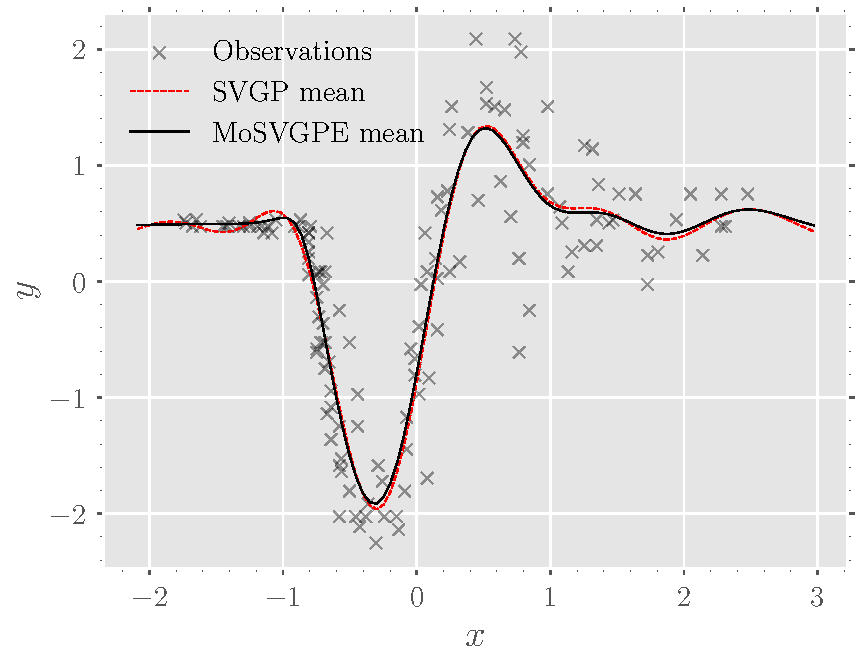
\includegraphics[width=\textwidth]{./images/model/mcycle/K=2_L2/y_means.pdf}
%\subcaption{Expert's latent function posteriors $\predictiveExpertPrior$ with $\ModeInd=2$.}
\subcaption{$\furtherBound$, poseterior mean and data set}
\label{fig-y-means-mcycle-two-experts-tight}
\end{minipage}
\begin{minipage}[r]{0.49\textwidth}
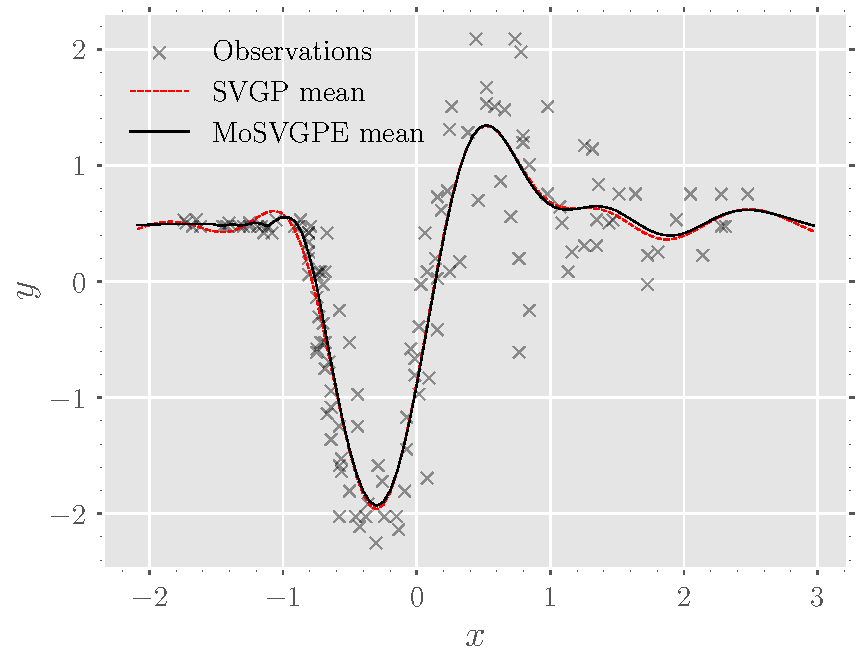
\includegraphics[width=\textwidth]{./images/model/mcycle/K=2_L3/y_means.pdf}
%\subcaption{Expert's latent function posteriors $\predictiveExpertPrior$ with $\ModeInd=3$.}
\subcaption{$\furtherBoundTwo$, poseterior mean and data set}
\label{fig-y-means-mcycle-two-experts-further}
\end{minipage}
\begin{minipage}[r]{0.49\textwidth}
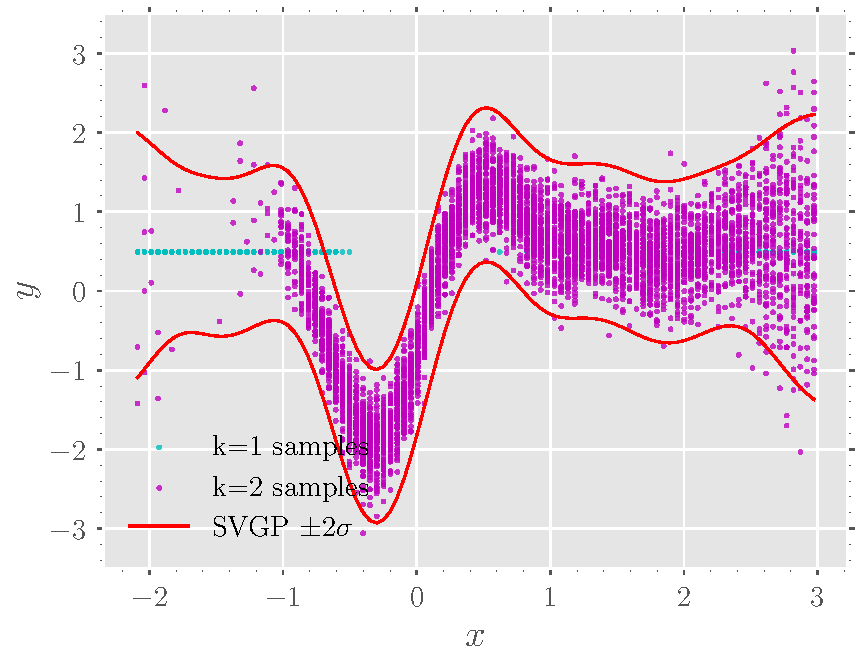
\includegraphics[width=\textwidth]{./images/model/mcycle/K=2_L2/y_samples.pdf}
\subcaption{$\furtherBound$, posterior samples}
\label{fig-y-samples-mcycle-two-experts-tight}
\end{minipage}
\begin{minipage}[r]{0.49\textwidth}
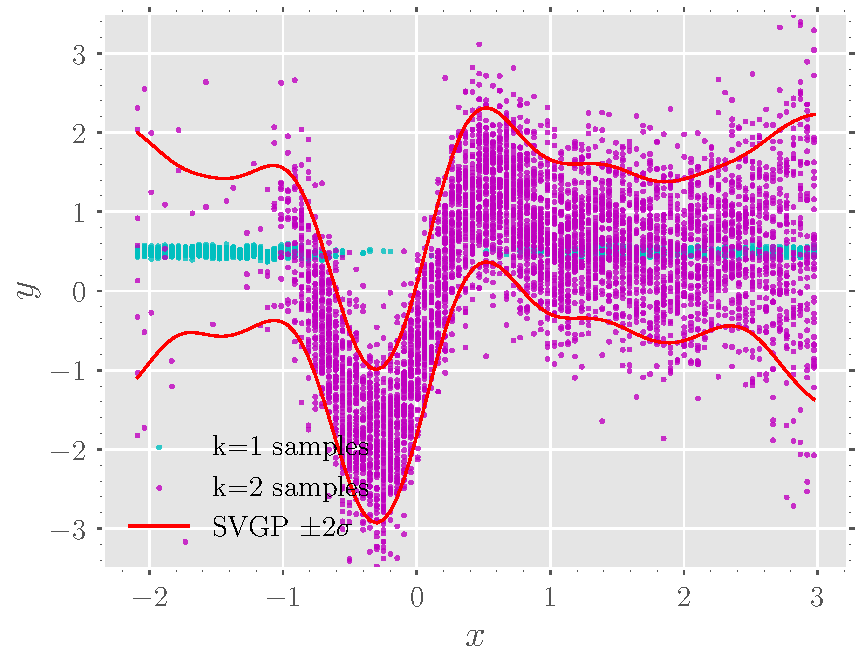
\includegraphics[width=\textwidth]{./images/model/mcycle/K=2_L3/y_samples.pdf}
\subcaption{$\furtherBoundTwo$, posterior samples}
\label{fig-y-samples-mcycle-two-experts-further}
\end{minipage}
%\begin{minipage}[r]{0.49\textwidth}
%\includegraphics[width=\textwidth]{./images/model/mcycle/K=2_L1/y_samples_density.pdf}
%\subcaption{}
%\label{fig-y-samples-mcycle-two-experts}
%\end{minipage}
%\begin{minipage}[r]{0.49\textwidth}
%\includegraphics[width=\textwidth]{./images/model/mcycle/K=2_L2/y_samples_density.pdf}
%\subcaption{}
%\label{fig-y-samples-mcycle-three-experts}
%\end{minipage}
\caption[\acrshort{mosvgpe}'s predictive posterior with $\ModeInd=2$ after training on motorcycle data set with $\furtherBound$ and $\furtherBoundTwo$]{Visualisation of the model instantiated with $\ModeInd=2$ experts, after training on the motorcycle data set \citep{Silverman1985} with $\furtherBound$ (left column) and with $\furtherBoundTwo$ (right column).  (\subref{fig-y-means-mcycle-two-experts-tight}-\subref{fig-y-means-mcycle-two-experts-further}) show the data set (black crosses) and the posterior means associated with the \acrshort{mosvgpe} (black solid line) and the \acrshort{svgp} (red dashed line) for comparison. (\subref{fig-y-samples-mcycle-two-experts-tight}-\subref{fig-y-samples-mcycle-two-experts-further}) show samples from the \acrshort{mosvgpe} posterior where colour indicates the underlying expert (cyan $K=1$, magenta $\ModeInd=2$) and the red lines show the $\pm 2$ standard deviation error ($95\%$ confidence interval) of the \acrshort{svgp} posterior. All experiments were trained with $25,000$ iterations of Adam \citep{kingmaAdam2017} using a learning rate of $0.01$ and a minibatch size of $\NumData_b=16$. All \acrshort{gps} use Squared Exponential kernels and $M=32$ inducing points.}
\label{fig-y-mcycle-two-experts}
\end{figure}

\subsubsection{Two Experts}
\label{sec:org9de263b}
The two further lower bounds (\(\furtherBound\) and \(\furtherBoundTwo\)),
derived in \cref{sec-inference}, are compared by training each instantiation of
the model using the same model and training parameters.
\cref{tab-params-motorcycle-two} contains the initial values for all of the trainable parameters in the model.
They are compared by instantiating the model with two experts \(\ModeInd=2\)
and comparing their performance.
The results are shown in \cref{fig-y-mcycle-two-experts,fig-latent-mcycle-two-experts},
where \cref{fig-y-mcycle-two-experts} visualises the predictive posteriors and
\cref{fig-latent-mcycle-two-experts} visualises the posteriors over the latent variables.
The left column shows results for \(\furtherBound\) and the right column shows results for \(\furtherBoundTwo\).
This layout is used in
\cref{fig-y-mcycle-two-experts,fig-latent-mcycle-two-experts,fig-y-mcycle-three-experts,fig-latent-mcycle-three-experts}.

\cref{fig-y-means-mcycle-two-experts-tight,fig-y-means-mcycle-two-experts-further}
compare the posterior means (black solid line) to the \acrshort{svgp}'s posterior mean (red dashed line) and
\cref{fig-y-samples-mcycle-two-experts-tight,fig-y-samples-mcycle-two-experts-further}
compare the posterior densities to the \acrshort{svgp}.
The red lines show plus or minus two standard deviations of the \acrshort{svgp}'s posterior variance.
As the \acrshort{mosvgpe} posterior is a Gaussian mixture, it is visualised by drawing samples
from its posterior, i.e. sample a mode indicator variable \(\modeVar_*\) and then draw a sample
from the corresponding expert.

\textbf{Predictive posteriors} Both \acrshort{mosvgpe} results are capable of modelling the non-stationarity
at \(x \approx -0.7\) better than the \acrshort{svgp}.
At this non-stationary point, there are two modes in the \acrshort{mosvgpe} predictive distributions,
indicated by the overlap in samples from each expert
in \cref{fig-y-samples-mcycle-two-experts-tight,fig-y-samples-mcycle-two-experts-further}.
The \acrshort{svgp} has explained the observations by increasing its single
noise variance term. In contrast, both of the \acrshort{mosvgpe} results have been able to learn
two noise variances and these reflect the noise in the observations much better.
This is indicated by expert one learning a low noise variance and expert two a high noise
variance (similar to the \acrshort{svgp}'s noise variance).

\textbf{Latent variables} More insight into this behaviour can be obtained by considering the latent variables.
Figure \ref{fig-latent-mcycle-two-experts} shows the posteriors over the latent variables where
\cref{fig-expert-gps-mcycle-two-experts-tight,fig-expert-gps-mcycle-two-experts-further}
show the \acrshort{gp} posteriors over each expert's latent function \(q(\mode{\latentFunc}(\x_*))\).
\cref{fig-gating-gps-mcycle-two-experts-tight,fig-gating-gps-mcycle-two-experts-further}
show the \acrshort{gp} posteriors over the latent gating functions \(q(\mode{\gatingFunc}(\x_*))\)
and \cref{fig-mixing-probs-mcycle-two-experts-tight,fig-mixing-probs-mcycle-two-experts-further}
show the mixing probabilities associated with the probability mass function over the expert
indicator variable \(\modeVar\).

The lengthscale of the gating network kernel governs how fast the model can shift responsibility from
expert one (cyan) to expert two (magenta).
For both lower bounds,
the distribution over the expert indicator variable tends to a uniform distribution (maximum entropy)
at \(x \geq 1.5\).
This can be seen by the cyan/magenta lines in
\cref{fig-mixing-probs-mcycle-two-experts-tight,fig-mixing-probs-mcycle-two-experts-further} tending to \(0.5\).
Optimising with both bounds resulted in expert one (cyan) learning a
long lengthscale to fit the horizontal line from \(-2<x<-1\) and
expert two (magenta) learning a shorter lengthscale function to fit the wiggly section from \(-0.5<x<1.2\).
The noise variance inferred by expert one is larger for \(\furtherBoundTwo\) than for \(\furtherBound\).
The uncertainty in the experts' latent functions is also higher for \(\furtherBoundTwo\).
This is shown by the \(95\%\) confidence intervals (shaded cyan/magenta) being wider in
\cref{fig-expert-gps-mcycle-two-experts-further} than in \cref{fig-expert-gps-mcycle-two-experts-tight}.
This is because \(\furtherBoundTwo\) is attempting to fit both experts to the entire data set and only
mixes their noise models.
In contrast, \(\furtherBound\) fits each expert only in the regions where the gating network has
assigned it responsibility.

%\begin{figure}[t!]
\begin{figure}[hbt!]
\centering
\begin{minipage}[r]{0.49\textwidth}
\centering
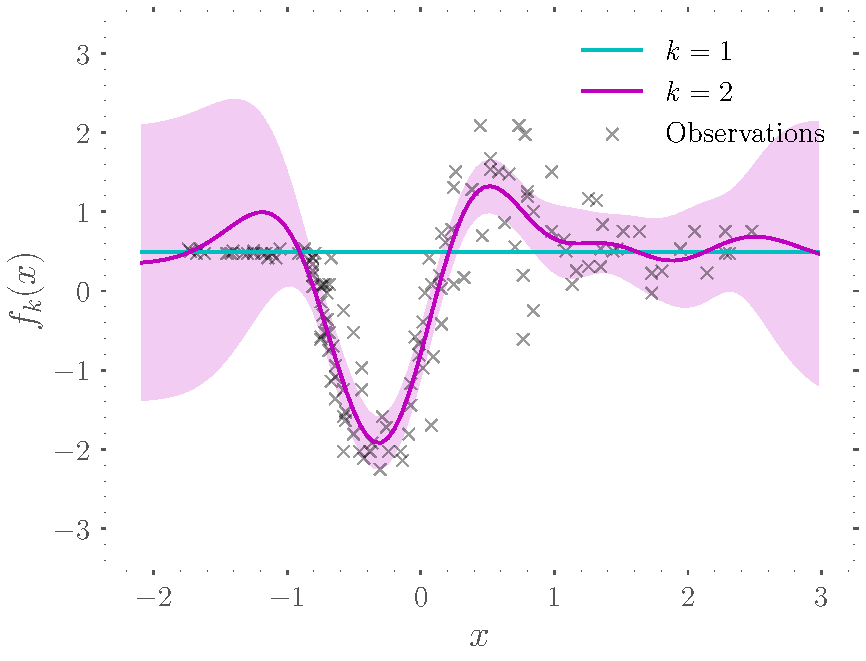
\includegraphics[width=\textwidth]{./images/model/mcycle/K=2_L2/experts_f.pdf}
%\subcaption{Expert's latent function posteriors $\predictiveExpertPrior$ with $\ModeInd=2$.}
\subcaption{$\furtherBound$, experts' \acrshort{gp} posteriors}
\label{fig-expert-gps-mcycle-two-experts-tight}
\end{minipage}
\begin{minipage}[r]{0.49\textwidth}
\centering
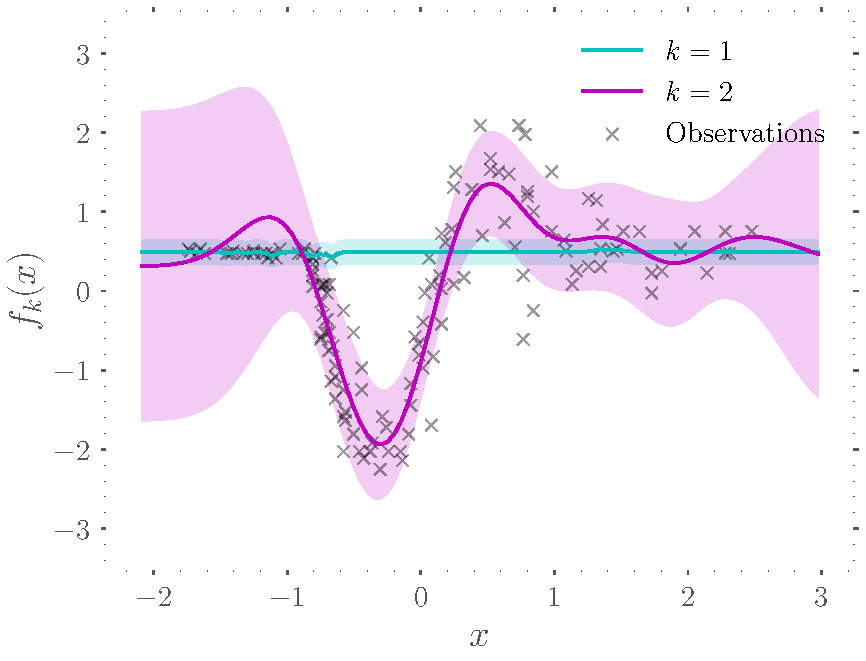
\includegraphics[width=\textwidth]{./images/model/mcycle/K=2_L3/experts_f.pdf}
%\subcaption{Expert's latent function posteriors $\predictiveExpertPrior$ with $\ModeInd=3$.}
\subcaption{$\furtherBoundTwo$, experts' \acrshort{gp} posteriors}
\label{fig-expert-gps-mcycle-two-experts-further}
\end{minipage}
\begin{minipage}[r]{0.49\textwidth}
\centering
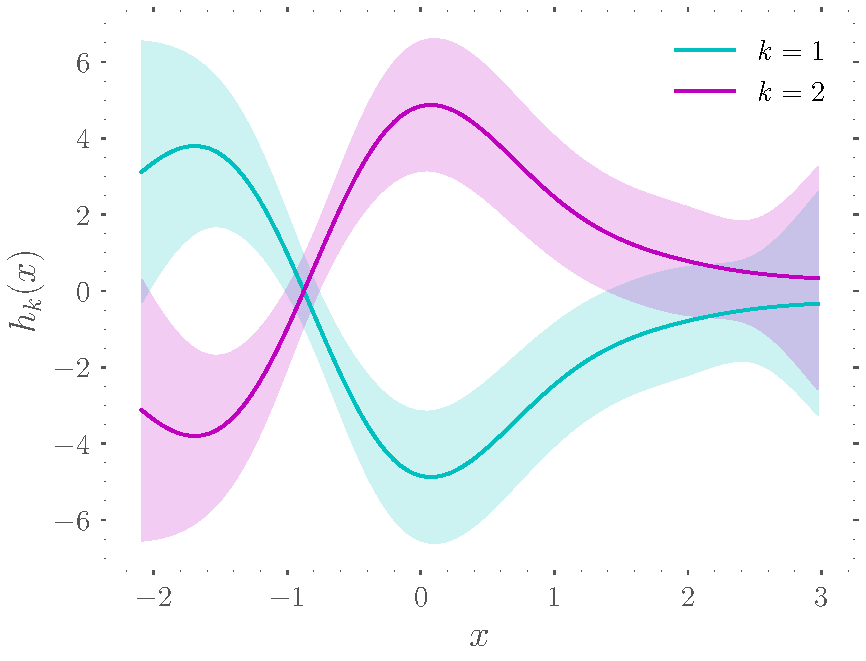
\includegraphics[width=\textwidth]{./images/model/mcycle/K=2_L2/gating_gps.pdf}
%\subcaption{Gating function posteriors $\predictiveGatingPrior$ with $\ModeInd=2$.}
\subcaption{$\furtherBound$, gating network's \acrshort{gp} posteriors}
\label{fig-gating-gps-mcycle-two-experts-tight}
\end{minipage}
\begin{minipage}[r]{0.49\textwidth}
\centering
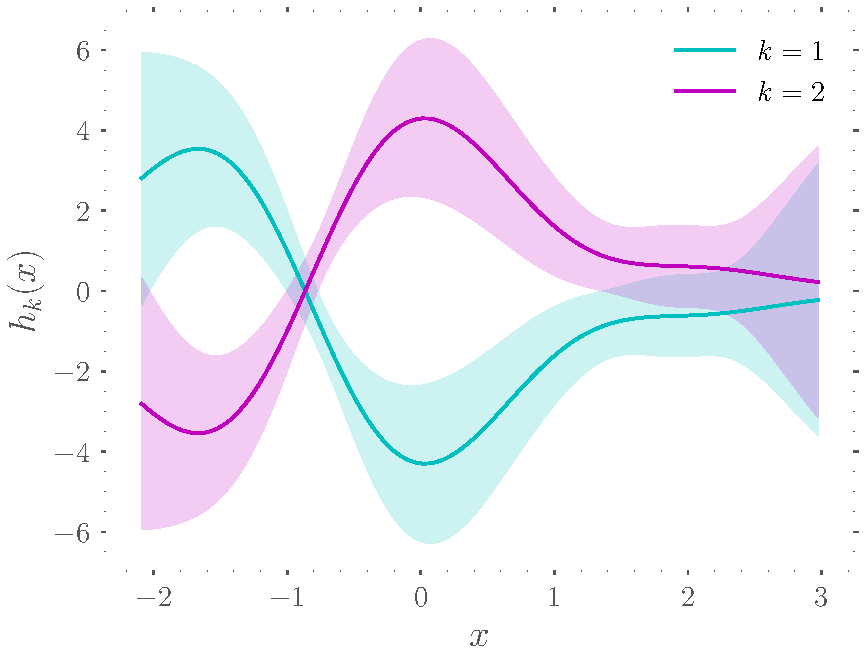
\includegraphics[width=\textwidth]{./images/model/mcycle/K=2_L3/gating_gps.pdf}
%\subcaption{Gating function posteriors $\predictiveGatingPrior$ with $\ModeInd=3$.}
\subcaption{$\furtherBoundTwo$, gating network's \acrshort{gp} posteriors}
\label{fig-gating-gps-mcycle-two-experts-further}
\end{minipage}
\begin{minipage}[r]{0.49\textwidth}
\centering
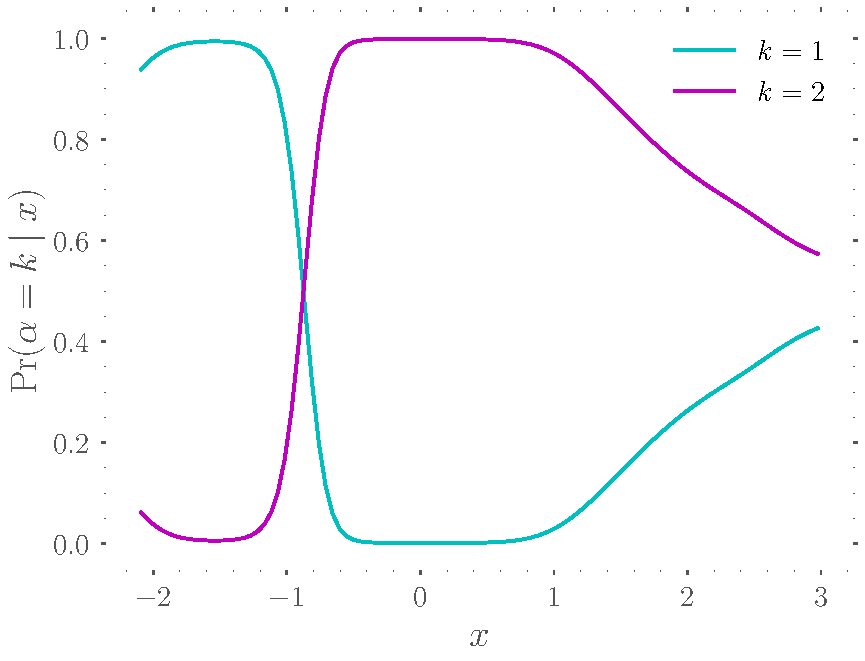
\includegraphics[width=\textwidth]{./images/model/mcycle/K=2_L2/gating_mixing_probs.pdf}
%\subcaption{Gating network's predictive mixing probabilities $\predictiveProb$ with $\ModeInd=2$.}
\subcaption{$\furtherBound$, mixing probabilities}
\label{fig-mixing-probs-mcycle-two-experts-tight}
\end{minipage}
\begin{minipage}[r]{0.49\textwidth}
\centering
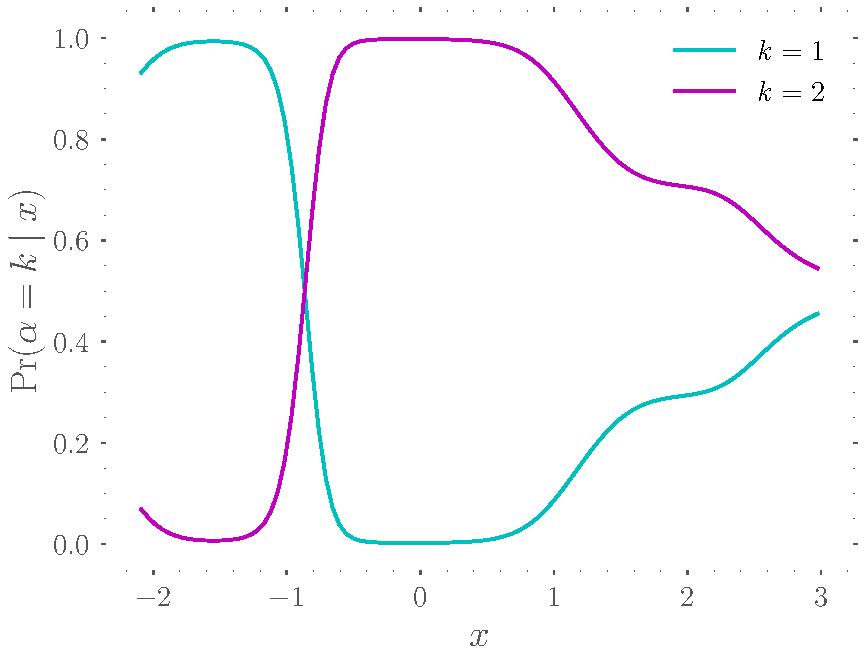
\includegraphics[width=\textwidth]{./images/model/mcycle/K=2_L3/gating_mixing_probs.pdf}
%\subcaption{Gating network's predictive mixing probabilities $\predictiveProb$ with $\ModeInd=3$.}
\subcaption{$\furtherBoundTwo$, mixing probabilities}
\label{fig-mixing-probs-mcycle-two-experts-further}
\end{minipage}
\caption[\acrshort{mosvgpe}'s latent variables' posteriors with $\ModeInd=2$ after training on motorcycle data set with $\furtherBound$ and $\furtherBoundTwo$]{Visualisation of the model's latent variables (instantiated with $\ModeInd=2$ experts), after training on the
Motorcycle data set \citep{Silverman1985}, with $\furtherBound$ (left column)
and with $\furtherBoundTwo$ (right column).
(\subref{fig-expert-gps-mcycle-two-experts-tight}-\subref{fig-expert-gps-mcycle-two-experts-further}) show the \acrshort{gp}
posteriors associated with the experts' latent functions $q(\mode{\latentFunc}(\x_*))$,
where the solid lines show the mean and the shaded regions show the $95\%$ confidence intervals, i.e. $\pm2\sigma$.
The gating network's \acrshort{gp} posteriors $q(h_{k}(\x_*))$ are shown in
(\subref{fig-gating-gps-mcycle-two-experts-tight}-\subref{fig-gating-gps-mcycle-two-experts-further}) and
their associated mixing probabilities $\approxPredictiveProb$ in
(\subref{fig-mixing-probs-mcycle-two-experts-tight}-\subref{fig-mixing-probs-mcycle-two-experts-further}).}
\label{fig-latent-mcycle-two-experts}
\end{figure}
\clearpage

\begin{table}
\caption{Initial parameter settings before training on motorcycle data set with three experts.}
\label{tab-params-motorcycle-three}
\resizebox{\textwidth}{!}{
\begin{center}
\begin{tabular}{llll}
 & Description & Symbol & Value\\
\hline
 & Num data & \(\NumData\) & \(133\)\\
 & Batch size & \(\NumData_b\) & \(16\)\\
Optimiser & Epochs & N/A & \(25000\)\\
 & Num gating samples & \(\hat{S}\) & \(1\)\\
 & Num expert samples & \(S\) & \(1\)\\
 & Learning rate & N/A & \(0.01\)\\
\hline
 & Kernel variance & \(\sigma_f\) & \(0.1\)\\
 & Kernel lengthscales & \(l\) & \(10\)\\
 & Likelihood variance & \(\sigma_n\) & \(0.03\)\\
Expert 1 & Num inducing points & \(\NumInducing\) & \(32\)\\
 & Inducing inputs & \(\expertsInducingInput_1\) & \(\expertsInducingInput_1 \subseteq \allInput\) with \(\#\expertsInducingInput_1 = \NumInducing\)\\
 & Inducing variable mean & \(\hat{\mathbf{m}}_1\) & zeros plus Gaussian noise\\
 & Inducing variable Cholesky & \(\hat{\mathbf{S}}_1\) & ones plus Gaussian noise\\
\hline
 & Kernel variance & \(\sigma_f\) & \(0.1\)\\
 & Kernel lengthscales & \(l\) & \(10.0\)\\
 & Likelihood variance & \(\sigma_n\) & \(0.1\)\\
Expert 2 & Num inducing points & \(\NumInducing\) & \(32\)\\
 & Inducing inputs & \(\expertsInducingInput_2\) & \(\expertsInducingInput_2 \subseteq \allInput\) with \(\#\expertsInducingInput_2 = \NumInducing\)\\
 & Inducing variable mean & \(\hat{\mathbf{m}}_2\) & zeros plus Gaussian noise\\
 & Inducing variable Cholesky & \(\hat{\mathbf{S}}_2\) & ones plus Gaussian noise\\
\hline
 & Kernel variance & \(\sigma_f\) & \(1.0\)\\
 & Kernel lengthscales & \(l\) & \(0.5\)\\
 & Likelihood variance & \(\sigma_n\) & \(0.9\)\\
Expert 3 & Num inducing points & \(\NumInducing\) & \(32\)\\
 & Inducing inputs & \(\expertsInducingInput_3\) & \(\expertsInducingInput_3 \subseteq \allInput\) with \(\#\expertsInducingInput_3 = \NumInducing\)\\
 & Inducing variable mean & \(\hat{\mathbf{m}}_3\) & zeros plus Gaussian noise\\
 & Inducing variable Cholesky & \(\hat{\mathbf{S}}_3\) & ones plus Gaussian noise\\
\hline
 & Kernel variance & \(\sigma_f\) & \(3.0\)\\
 & Kernel lengthscales & \(l\) & \(0.5\)\\
Gating functions (1-3) & Num inducing points & \(\NumInducing\) & \(32\)\\
 & Inducing inputs & \(\gatingInducingInput\) & \(\gatingInducingInput \subseteq \allInput\) with \(\#\gatingInducingInput = \NumInducing\)\\
 & Inducing variable mean & \(\mode{\hat{\mathbf{m}}}\) & zeros plus Gaussian noise\\
 & Inducing variable Cholesky & \(\mode{\hat{\mathbf{S}}}\) & \(10 \times\) ones plus Gaussian noise\\
\hline
\end{tabular}
\end{center}
}
\end{table}

\begin{figure}[t!]
\centering
\begin{minipage}[r]{0.49\textwidth}
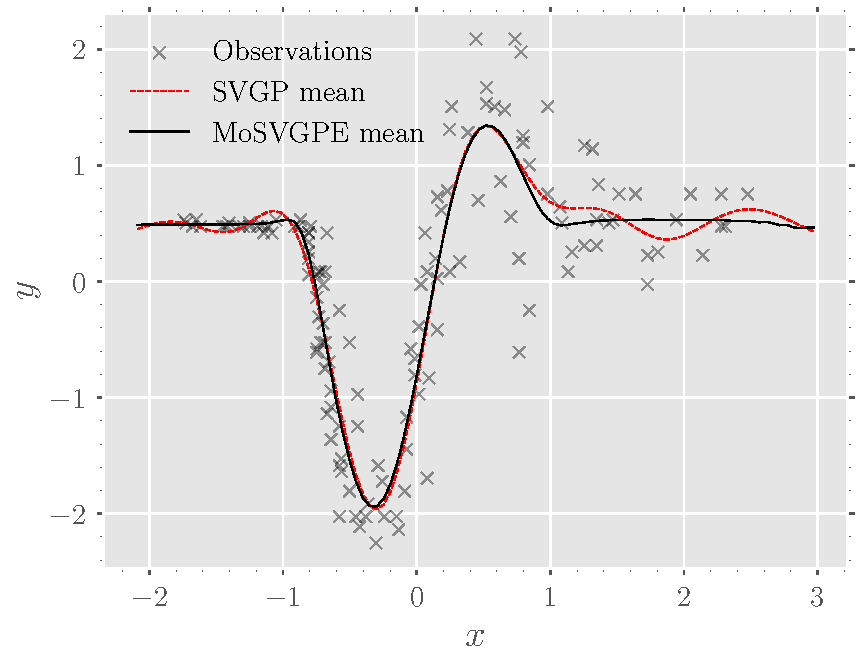
\includegraphics[width=\textwidth]{./images/model/mcycle/K=3_L2/y_means.pdf}
\subcaption{$\furtherBound$, poseterior mean and data set}
\label{fig-y-means-three-experts-tight}
\end{minipage}
\begin{minipage}[r]{0.49\textwidth}
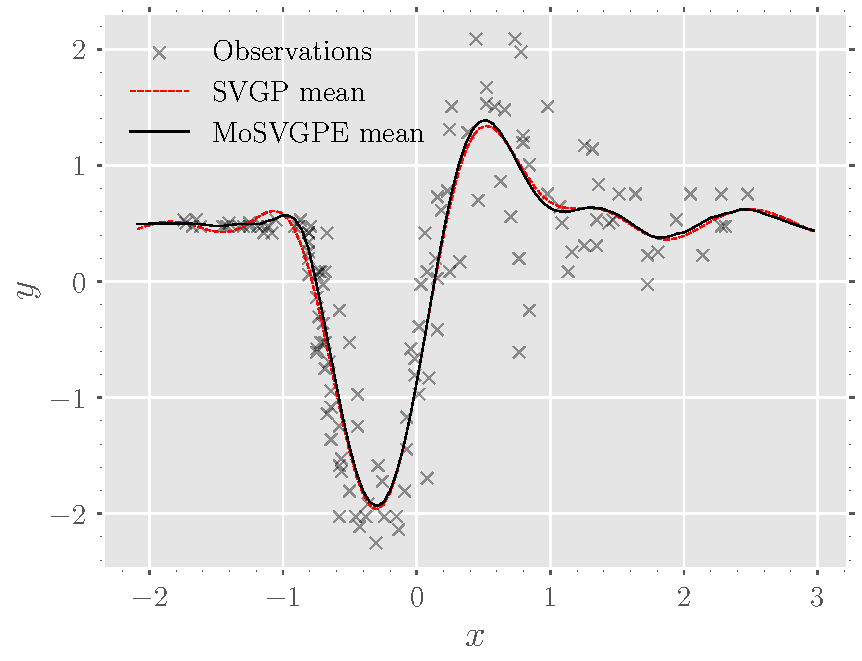
\includegraphics[width=\textwidth]{./images/model/mcycle/K=3_L3/y_means.pdf}
\subcaption{$\furtherBoundTwo$, poseterior mean and data set}
\label{fig-y-means-three-experts-further}
\end{minipage}
\begin{minipage}[r]{0.49\textwidth}
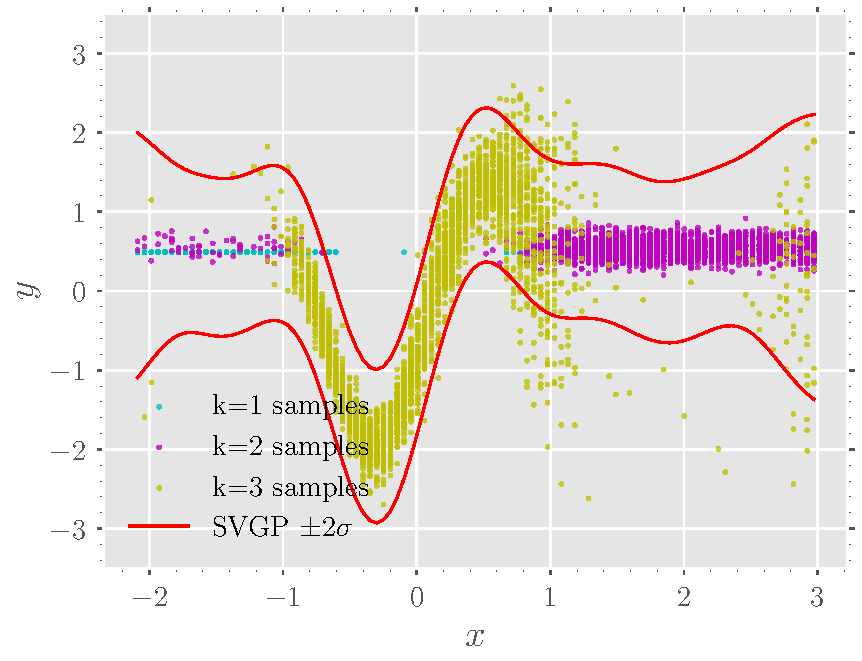
\includegraphics[width=\textwidth]{./images/model/mcycle/K=3_L2/y_samples.pdf}
\subcaption{$\furtherBound$, posterior samples}
\label{fig-y-samples-mcycle-three-experts-tight}
\end{minipage}
\begin{minipage}[r]{0.49\textwidth}
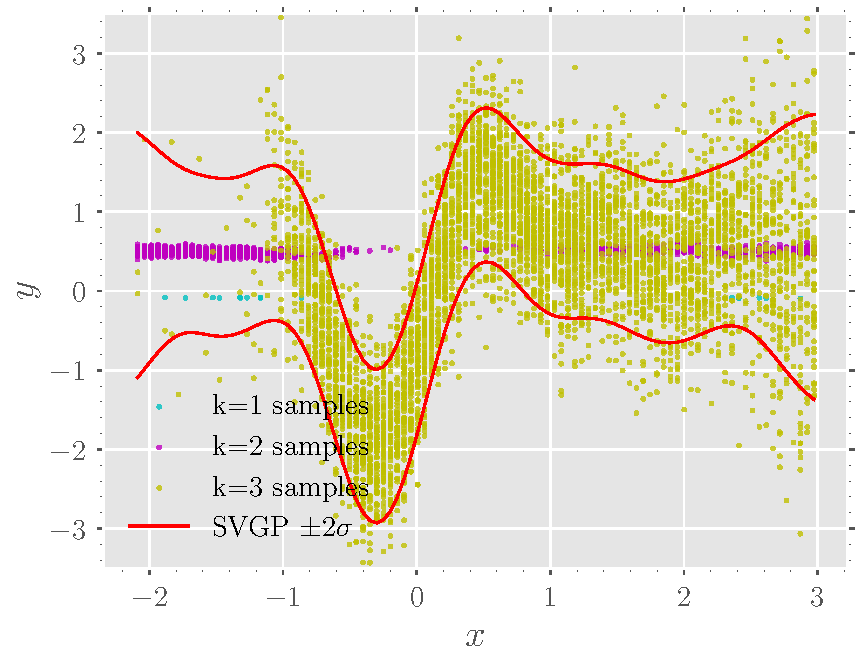
\includegraphics[width=\textwidth]{./images/model/mcycle/K=3_L3/y_samples.pdf}
\subcaption{$\furtherBoundTwo$, posterior samples}
\label{fig-y-samples-mcycle-three-experts-further}
\end{minipage}
%\begin{minipage}[r]{0.49\textwidth}
%\includegraphics[width=\textwidth]{./images/model/mcycle/K=3_L1/y_samples_density.pdf}
%\subcaption{}
%\label{fig-y-samples-mcycle-two-experts}
%\end{minipage}
%\begin{minipage}[r]{0.49\textwidth}
%\includegraphics[width=\textwidth]{./images/model/mcycle/K=3_L2/y_samples_density.pdf}
%\subcaption{}
%\label{fig-y-samples-mcycle-three-experts}
%\end{minipage}
\caption[\acrshort{mosvgpe}'s predictive posterior with $\ModeInd=3$ after training on motorcycle data set with $\furtherBound$ and $\furtherBoundTwo$]{Visualisation of the model instantiated with $\ModeInd=3$ experts, after training on the motorcycle data set \citep{Silverman1985} with $\furtherBound$ (left column) and with $\furtherBoundTwo$ (right column).  (\subref{fig-y-means-three-experts-tight}-\subref{fig-y-means-three-experts-further}) show the data set (black crosses) and the posterior means associated with the \acrshort{mosvgpe} (black solid line) and the \acrshort{svgp} (red dashed line) for comparison. (\subref{fig-y-samples-mcycle-three-experts-tight}-\subref{fig-y-samples-mcycle-three-experts-further}) show samples from the \acrshort{mosvgpe} posterior where colour indicates the underlying expert (cyan $K=1$, magenta $\ModeInd=2$, yellow $\ModeInd=3$) and the red lines show the $\pm 2$ standard deviation error ($95\%$ confidence interval) of the \acrshort{svgp} posterior. All experiments were trained with $25,000$ iterations of Adam \citep{kingmaAdam2017} using a learning rate of $0.01$ and a minibatch size of $\NumData_b=16$. All \acrshort{gps} use Squared Exponential kernels and $M=32$ inducing points.}
\label{fig-y-mcycle-three-experts}
\end{figure}

\subsubsection{Three Experts}
\label{sec:org46df5ab}
The model was then instantiated with three experts \(\ModeInd=3\) and trained
following the same procedure as the two experts' experiments.
\cref{tab-params-motorcycle-three} shows the initial values for all of the trainable parameters in the model.
The results are shown in \cref{fig-y-mcycle-three-experts},
where the top row visualises the predictive mean and
the bottom row the predictive density, for \(\furtherBound\) (left column) and \(\furtherBoundTwo\) (right column).
\cref{fig-latent-mcycle-three-experts} then visualises the posteriors over the latent variables associated with
each model/bound combination.

From \cref{tab-mcycle-metrics}, it is clear that the predictive posterior associated with \(\furtherBound\)
is the most accurate as it obtained the best \acrshort{nlpp} score.
As expected, the two lower bounds explain the data completely differently.
Instantiating the model with three experts \(\ModeInd=3\) and training with \(\furtherBound\),
leads to the extra expert (magenta) fitting to the data at \(x \geq 1.5\) and the gating network
assigning responsibility to it in this region.
In contrast, instantiating the model with three experts \(\ModeInd=3\) and training with
\(\furtherBoundTwo\), results in the gating network never using the extra expert (cyan).
This is indicated by the extra expert's (cyan) probability remaining low over the region with training data in
\cref{fig-mixing-probs-mcycle-three-experts-further}.
Similar to the two expert case, the distribution over the expert indicator variable at \(x \geq 1.5\)
tends to a uniform distribution (maximum entropy), over the experts that are turned ``on''.

In \cref{fig-expert-gps-mcycle-three-experts-tight} the third expert's posterior returns to the prior at
\(x \geq 1.5\).
This is indicated by the \(95\%\) confidence intervals associated with the third expert's \acrshort{gp} (shaded yellow)
being wide in this region.
This demonstrates that not only is the gating network turning the experts ``on'' and ``off'' in different regions
but the model is also exhibiting data assignment behaviour.
That is, each expert appears to only be fitting to the observations in the regions where the gating network
has assigned it responsibility.
In our case, this behaviour is achieved via the inducing variables capturing the joint distribution over the
experts and the set of assignments, i.e. implicitly assigning data points to experts.

\begin{figure}[hbt!]
\centering
\begin{minipage}[r]{0.49\textwidth}
\centering
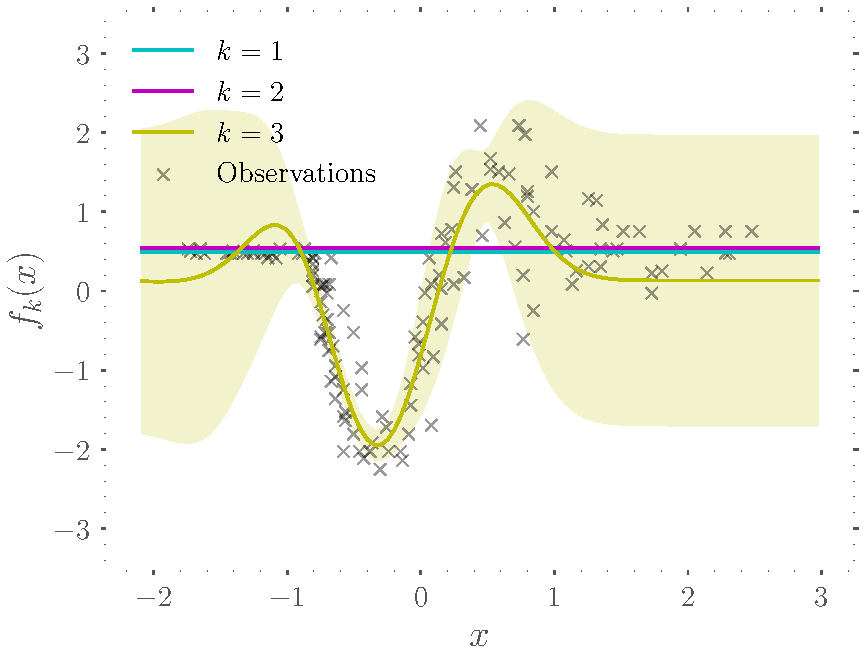
\includegraphics[width=\textwidth]{./images/model/mcycle/K=3_L2/experts_f.pdf}
\subcaption{$\furtherBound$, experts' \acrshort{gp} posteriors}
\label{fig-expert-gps-mcycle-three-experts-tight}
\end{minipage}
\begin{minipage}[r]{0.49\textwidth}
\centering
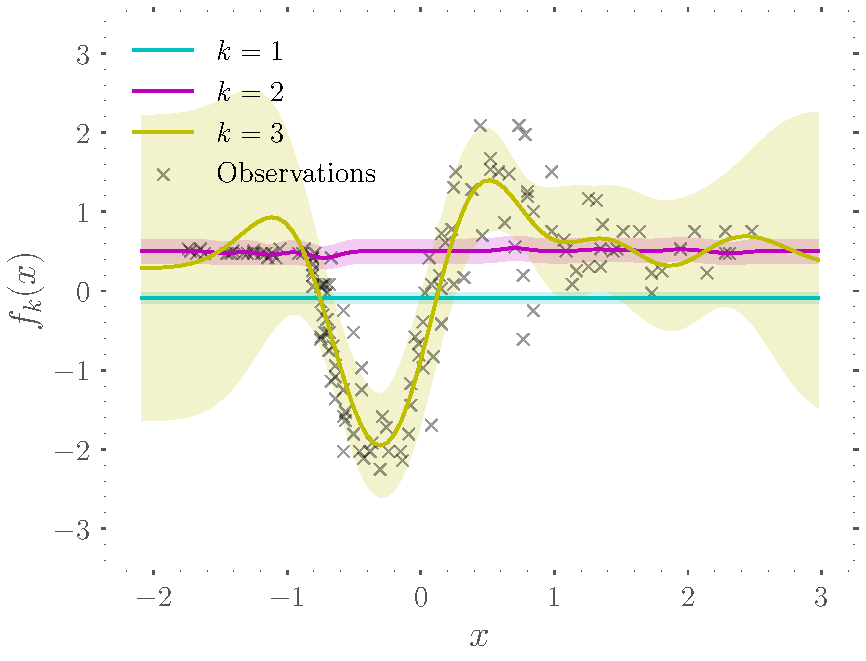
\includegraphics[width=\textwidth]{./images/model/mcycle/K=3_L3/experts_f.pdf}
\subcaption{$\furtherBoundTwo$, experts' \acrshort{gp} posteriors}
\label{fig-expert-gps-mcycle-three-experts-further}
\end{minipage}
\begin{minipage}[r]{0.49\textwidth}
\centering
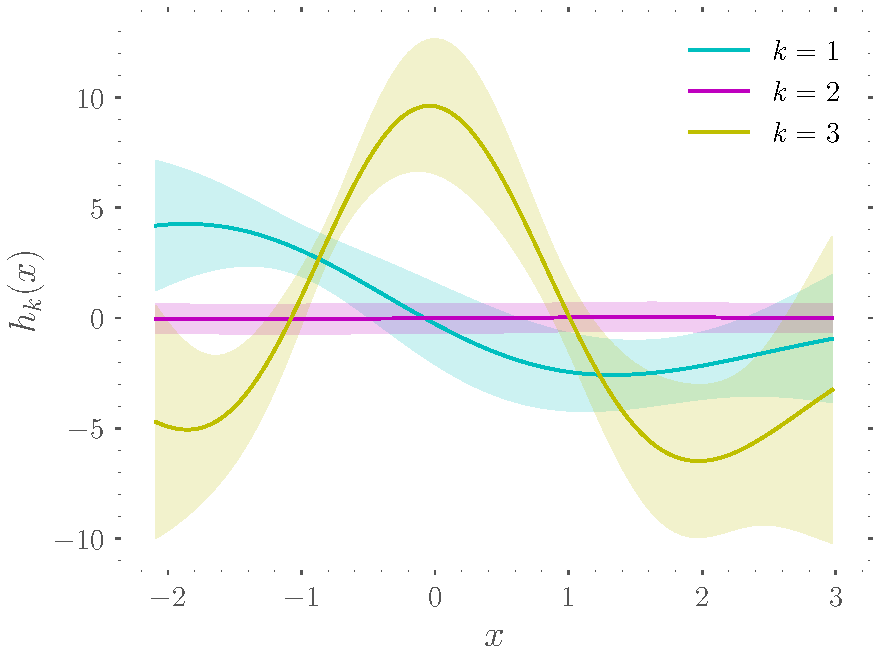
\includegraphics[width=\textwidth]{./images/model/mcycle/K=3_L2/gating_gps.pdf}
\subcaption{$\furtherBound$, gating network's \acrshort{gp} posteriors}
\label{fig-gating-gps-mcycle-three-experts-tight}
\end{minipage}
\begin{minipage}[r]{0.49\textwidth}
\centering
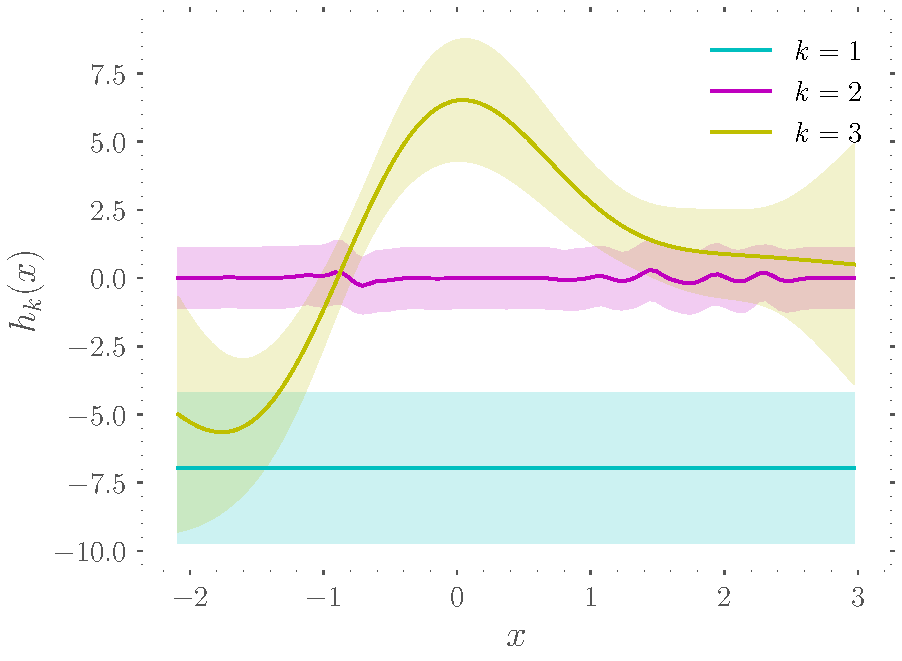
\includegraphics[width=\textwidth]{./images/model/mcycle/K=3_L3/gating_gps.pdf}
\subcaption{$\furtherBoundTwo$, gating network's \acrshort{gp} posteriors}
\label{fig-gating-gps-mcycle-three-experts-further}
\end{minipage}
\begin{minipage}[r]{0.49\textwidth}
\centering
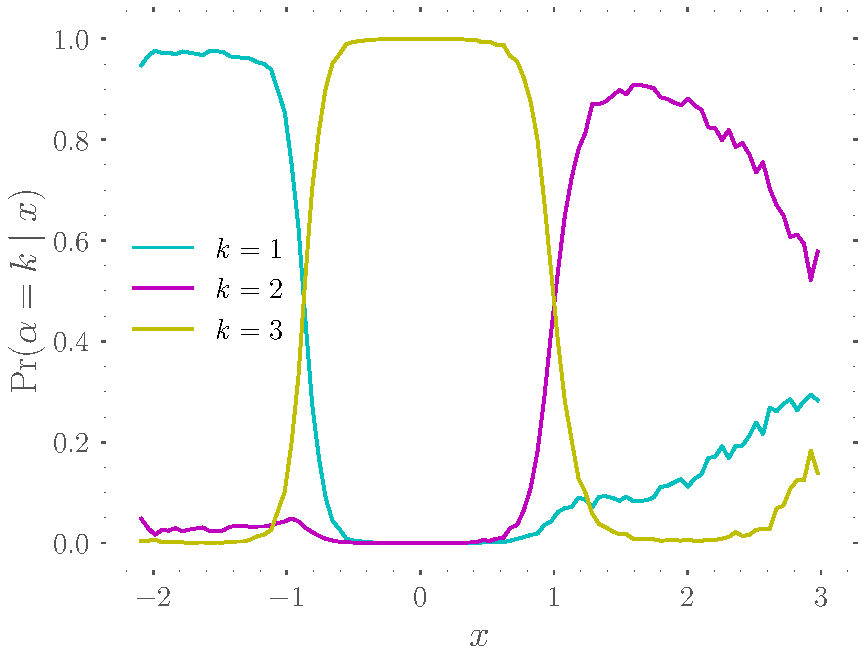
\includegraphics[width=\textwidth]{./images/model/mcycle/K=3_L2/gating_mixing_probs.pdf}
\subcaption{$\furtherBound$, mixing probabilities}
\label{fig-mixing-probs-mcycle-three-experts-tight}
\end{minipage}
\begin{minipage}[r]{0.49\textwidth}
\centering
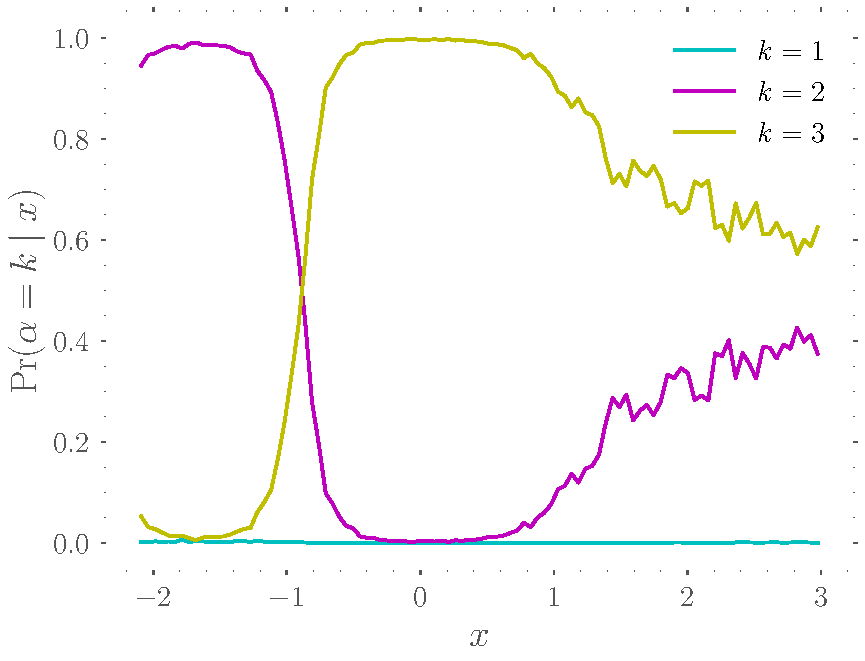
\includegraphics[width=\textwidth]{./images/model/mcycle/K=3_L3/gating_mixing_probs.pdf}
%\subcaption{Gating network's predictive mixing probabilities $\predictiveProb$ with $\ModeInd=3$.}
\subcaption{$\furtherBoundTwo$, mixing probabilities}
\label{fig-mixing-probs-mcycle-three-experts-further}
\end{minipage}
\caption[\acrshort{mosvgpe}'s latent variables' posteriors with $\ModeInd=3$ after training on motorcycle data set with $\furtherBound$ and $\furtherBoundTwo$]{Visualisation of the model's latent variables (instantiated with $\ModeInd=3$ experts), after training on the
Motorcycle data set \citep{Silverman1985}, with $\furtherBound$ (left column)
and with $\furtherBoundTwo$ (right column).
(\subref{fig-expert-gps-mcycle-three-experts-tight}-\subref{fig-expert-gps-mcycle-three-experts-further}) show the \acrshort{gp}
posteriors associated with the experts' latent functions $q(\mode{\latentFunc}(\state_*))$,
where the solid lines show the mean and the shaded regions show the $95\%$ confidence intervals, i.e. $\pm2\sigma$.
The gating network's \acrshort{gp} posteriors $q(h_{k}(\state_*))$ are shown in
(\subref{fig-gating-gps-mcycle-three-experts-tight}-\subref{fig-gating-gps-mcycle-three-experts-further}) and
their associated mixing probabilities $\approxPredictiveProb$ in
(\subref{fig-mixing-probs-mcycle-three-experts-tight}-\subref{fig-mixing-probs-mcycle-three-experts-further}).}
\label{fig-latent-mcycle-three-experts}
\end{figure}
\clearpage

\subsubsection{Summary}
\label{sec:orgdda56d9}
The tight lower bound \(\tightBound\) and further lower bound \(\furtherBound\) recovered similar results in
all experiments.
This indicates that \(\furtherBound\) does not loosen the bound to a point where it loses valuable information.
In contrast, \(\furtherBoundTwo\) is not able to recover the same results.
This was expected as \(\furtherBoundTwo\) corresponds to a further likelihood approximation, where
the experts' noise models are mixed instead of their full \acrshort{svgp}s.
\(\furtherBound\) offers a rich \acrshort{elbo} for optimising \acrshort{mosvgpe} that achieves similar results to \(\tightBound\),
whilst having lower computational complexity per evaluation.
For this reason, the remainder of this thesis uses \(\furtherBound\) for all experiments.

\newpage

\subsection{Evaluation on Velocity Controlled Quadcopter \label{sec-brl-experiment}}
\label{sec:orga4b0ee8}
As this work is motivated by learning representations of real-world dynamical systems, it was
tested on a real-world quadcopter data set following the illustrative example detailed
in \cref{illustrative_example}.
The data set was collected at the Bristol Robotics Laboratory using
a velocity controlled DJI Tello quadcopter and a Vicon tracking system.
A high turbulence dynamics mode was induced by placing a desktop fan at the right side of a room.
\cref{fig-quadcopter-environment} shows a diagram of the environment.
The data set represents samples from a dynamical system with constant controls, i.e.
\(\Delta\state_{\timeInd+1} = \latentFunc(\state_{\timeInd};\control_{\timeInd}=\control_*)\).

\begin{figure}[h]
\centering
\begin{minipage}[r]{0.55\columnwidth}
\centering
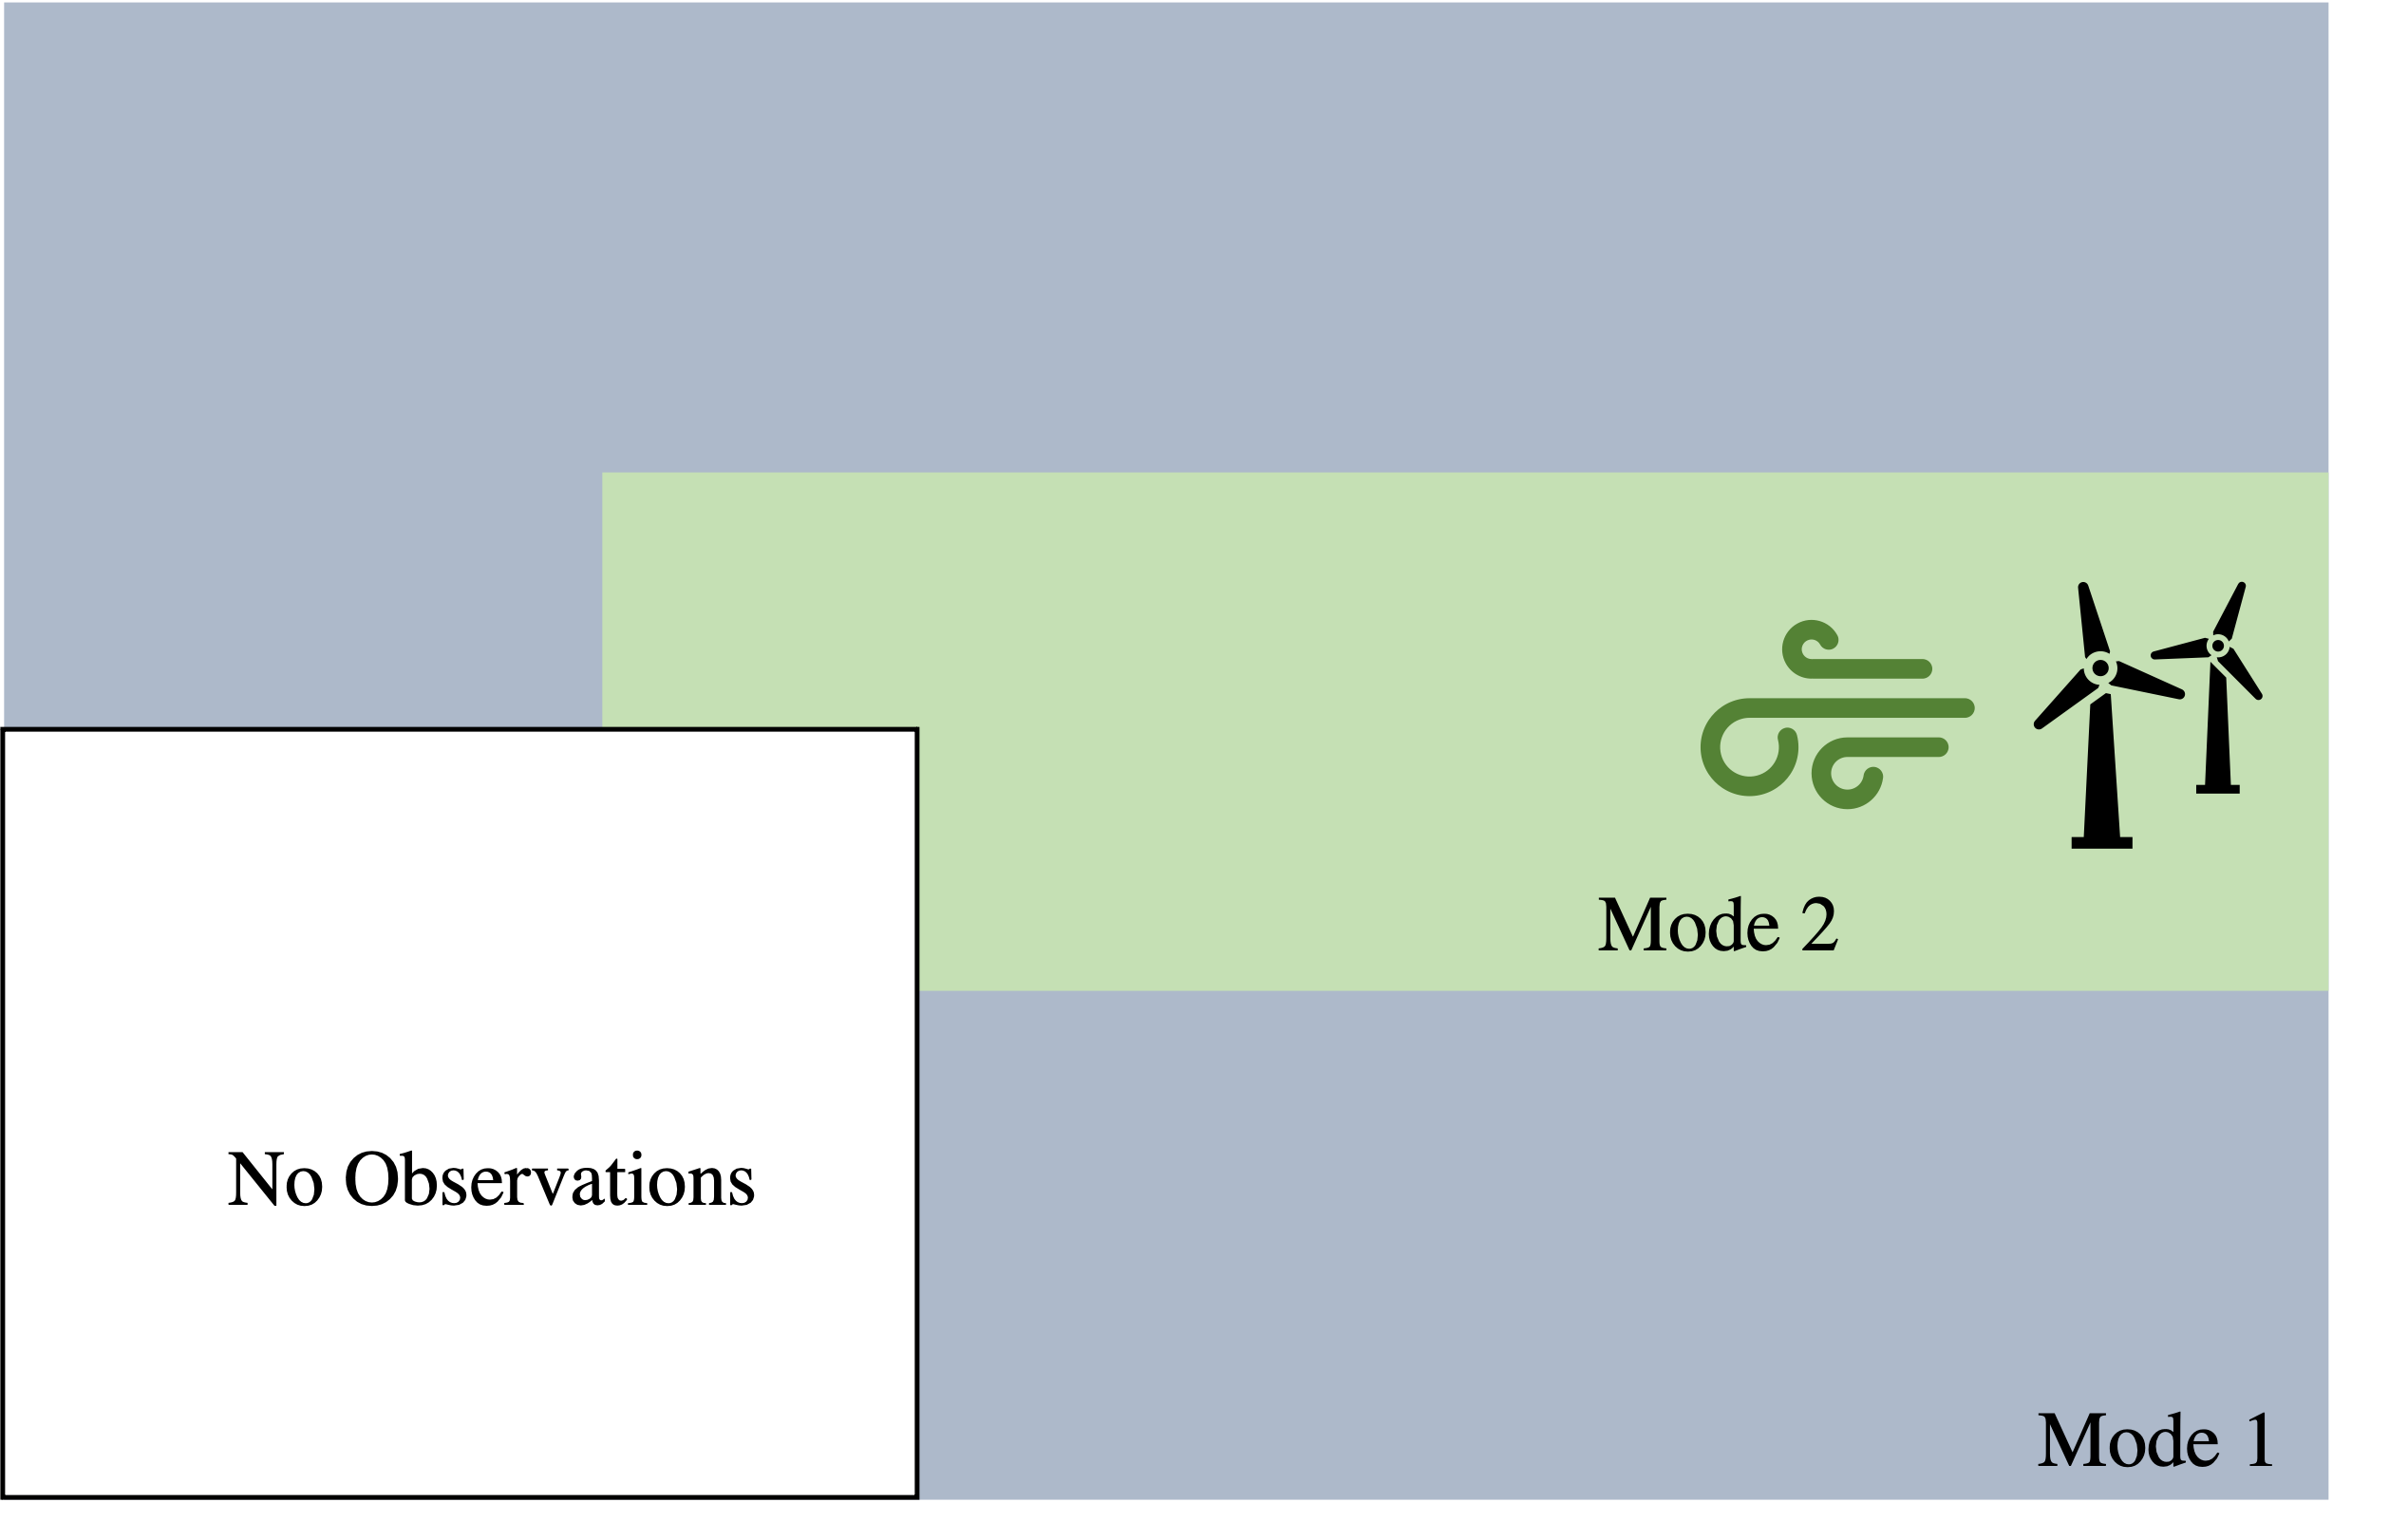
\includegraphics[width=\textwidth]{./images/brl-quadcopter-domain-figure.png}
\subcaption{Diagram showing a top-down view of the environment (a room in the \acrfull{brl}).}
\label{fig-quadcopter-environment}
\end{minipage}
\begin{minipage}[r]{0.44\columnwidth}
%\includegraphics[width=\textwidth]{./images/quiver_step_20_direction_down.png}
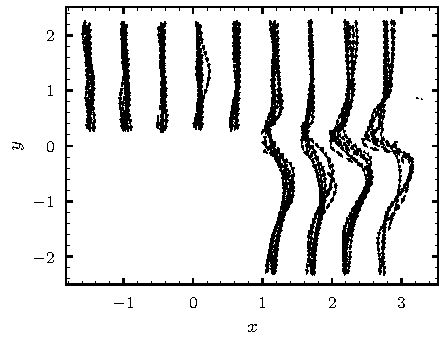
\includegraphics[width=\textwidth]{./images/model/quadcopter/subset-10/dataset_quiver.pdf}
\subcaption{Quiver plot showing the data set of state transitions from 9 trajectories flown 7 times.}
\label{fig-quiver}
\end{minipage}
\caption[Diagram of the real-world quadcotper environment and the state transition data set]{Illustration of (\subref{fig-quadcopter-environment}) the environment (a room in the \acrfull{brl}) and (\subref{fig-quiver}) the data set of state transitions. A turbulent dynamics mode is induced by a desk top fan at the right-hand side of the room and a subset of the environment has not been observed.}
\end{figure}


\textbf{Environment} The environment is modelled with two dimensions
(the \(x\) and \(y\) coordinates), which is a realistic assumption,
as altitude control can be achieved with a separate controller.
The state space is then the 2D coordinates \(\state = [x, y]\) and the control is simply the velocity
\(\control = [v_x, v_y]\).

\textbf{Data collection} The Vicon system provided access to the true position of the quadcopter at all times, which
enabled pre-planned trajectories to be flown, using a simple \acrshort{pid} controller on
feedback from the Vicon system.
To simplify data collection,
nine trajectories from \(y=2\) to \(y=-3\), with different initial \(x\) locations,
were used as target trajectories to be tracked by the \acrshort{pid} controller.
Each trajectory was repeated 7 times to capture the variability (process noise) in the dynamics.

\textbf{Data processing} The Vicon stream recorded data at 100Hz, which was then downsampled to
give a time step of \(\Delta t = 0.1s\).
This reduced the size of the data set and left reasonable lengthscales.
The data set consists of \(\NumData=1816\) state transitions.
\cref{fig-quiver} visualises the state transition data set as a quiver plot.

\begin{table}
\caption{Initial parameter settings before training on the real-world velocity controlled quadcopter data set.}
\label{tab-params-quadcopter}
\resizebox{\textwidth}{!}{
\begin{tabular}{llll}
 & Description & Symbol & Value\\
\hline
 & Num data & \(\NumData\) & \(1816\)\\
 & Batch size & \(\NumData_b\) & \(64\)\\
Optimiser & Num epochs & N/A & \(10000\)\\
 & Num gating samples & \(\hat{S}\) & \(1\)\\
 & Num expert samples & \(S\) & \(1\)\\
 & Learning rate & N/A & \(0.01\)\\
\hline
 & Constant mean function & \(c_1\) & \([0,0]\)\\
 & Kernel variance & \(\sigma_f\) & \(0.1\)\\
 & Kernel lengthscales & \(l\) & \([2, 2]\)\\
 & Likelihood variance & \(\Sigma_{\epsilon_1}\) & \(\diag([0.0011, 0.0011])\)\\
Expert 1 & Num inducing points & \(\NumInducing\) & \(100\)\\
 & Inducing inputs & \(\expertsInducingInput_1\) & \(\expertsInducingInput_1 \subseteq \allInput\) with \(\#\expertsInducingInput_1 = \NumInducing\)\\
 & Inducing variable mean & \(\hat{\mathbf{m}}_1\) & zeros plus Gaussian noise\\
 & Inducing variable Cholesky & \(\hat{\mathbf{S}}_1\) & ones plus Gaussian noise\\
\hline
 & Constant mean function & \(c_2\) & \([0,0]\)\\
 & Kernel variance & \(\sigma_f\) & \(20\)\\
 & Kernel lengthscales & \(l\) & \([0.5, 0.5]\)\\
 & Likelihood variance & \(\Sigma_{\epsilon_2}\) & \(\diag([1.9,1.9])\)\\
Expert 2 & Num inducing points & \(\NumInducing\) & \(100\)\\
 & Inducing inputs & \(\expertsInducingInput_2\) & \(\expertsInducingInput_2 \subseteq \allInput\) with \(\#\expertsInducingInput_2 = \NumInducing\)\\
 & Inducing variable mean & \(\hat{\mathbf{m}}_2\) & zeros plus Gaussian noise\\
 & Inducing variable Cholesky & \(\hat{\mathbf{S}}_2\) & ones plus Gaussian noise\\
\hline
 & Kernel variance & \(\sigma_f\) & \(0.6\)\\
 & Kernel lengthscales & \(l\) & \([0.1, 0.1]\)\\
Gating function & Num inducing points & \(\NumInducing\) & \(100\)\\
 & Inducing inputs & \(\expertInducingInput\) & \(\expertInducingInput \subseteq \allInput\) with \(\#\expertInducingInput = \NumInducing\)\\
 & Inducing variable mean & \(\mode{\hat{\mathbf{m}}}\) & zeros plus Gaussian noise\\
 & Inducing variable Cholesky & \(\mode{\hat{\mathbf{S}}}\) & \(2 \times\) ones plus Gaussian noise\\
\hline
\end{tabular}
}
\end{table}

\subsubsection{Results}
\label{sec:orgc3e78ea}
The model was instantiated with two experts, with the goal of each expert learning a separate dynamics mode and the
gating network learning a representation of how the underlying dynamics modes vary over the state space.
The model was trained using the model and training parameters in \cref{tab-params-quadcopter}.

\begin{figure}[t]
\centering
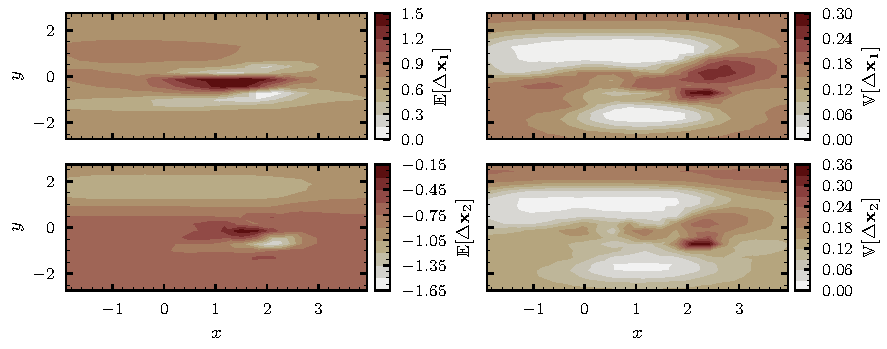
\includegraphics[width=1\textwidth]{./images/model/quadcopter/subset-10/y_moment_matched.pdf}
\caption[\acrshort{mosvgpe}'s moment matched predictive posterior with \(\ModeInd=2\) after training on the real-world quadcopter data set with \(\furtherBound\)]{\label{fig-y-mm-quadcopter-subset}Moment matched predictive posterior \(p(\Delta \state_* \mid \x_*)\) after training on the quadcopter data set. Each row corresponds to an output dimension \(d\) where the left plot shows the moment matched mean \(\E[\Delta \state_d]\) and the right plot shows the moment matched variance \(\V[\Delta \state_d]\).}
\end{figure}

\begin{figure}[t1]
\centering
\begin{minipage}[r]{1.0\textwidth}
\centering
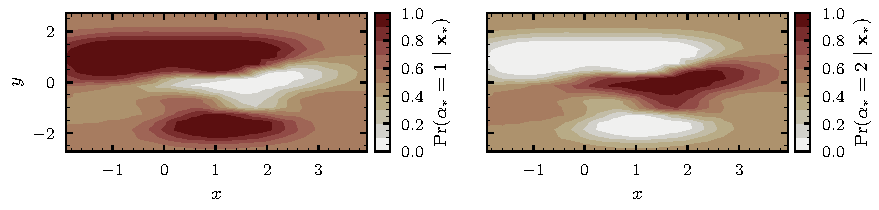
\includegraphics[width=\textwidth]{./images/model/quadcopter/subset-10/gating_mixing_probs.pdf}
\subcaption{Posterior over mode indicator variable.}
\label{fig-gating-mixing-probs-quadcopter-subset}
\end{minipage}
\begin{minipage}[r]{1.0\textwidth}
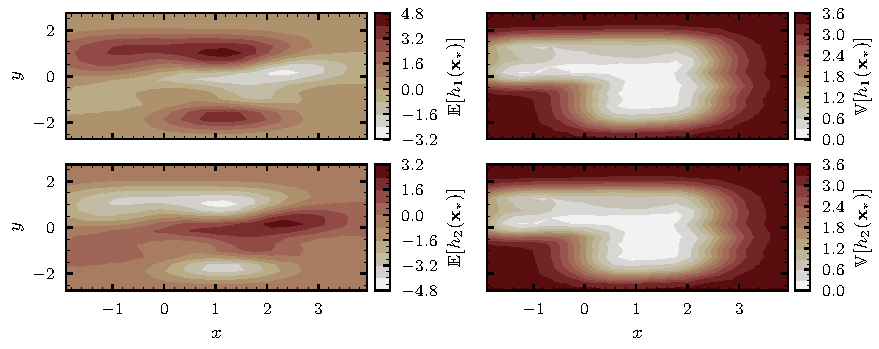
\includegraphics[width=\textwidth]{./images/model/quadcopter/subset-10/gating_gps.pdf}
\subcaption{\acrshort{gp} posteriors over gating functions.}
\label{fig-gating-gps-quadcopter-subset}
\end{minipage}
\caption[\acrshort{mosvgpe}'s gating network posterior with $\ModeInd=2$ after training on the real-world quadcopter data set with $\furtherBound$]{Visualisation of the gating network after training on the quadcopter data set. The plots in (\subref{fig-gating-mixing-probs-quadcopter-subset}) show the predictive mixing probabilities $\predictiveProb$ for Expert 1 (left) and Expert 2 (right). The plots in (\subref{fig-gating-gps-quadcopter-subset}) show the predictive \acrshort{gp} posteriors $q(h_{k}(\singleTestInput))$ associated with Expert 1 (top) and Expert 2 (bottom). The left-hand plots show the means and the right-hand plots show the variances.}
\label{fig-gating-network-quadcopter-subset}
\end{figure}

\begin{figure}[t!]
\centering
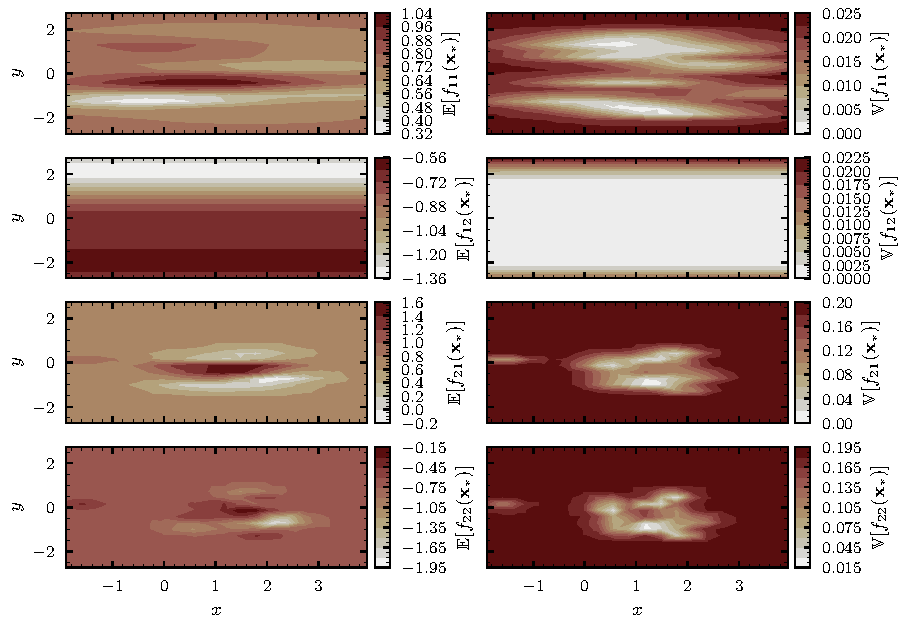
\includegraphics[width=1\textwidth]{./images/model/quadcopter/subset-10/experts_f.pdf}
\caption[\acrshort{mosvgpe}'s experts' posteriors with \(\ModeInd=2\) after training on the real-world quadcopter data set with \(\furtherBound\)]{\label{fig-experts-f-quadcopter-subset}Visualisation of the experts' predictive posteriors \(\predictiveExpertsPrior\) after training on the quadcopter data set. Each row corresponds to a single \acrshort{gp} posterior, \(q(f_{kd}(\singleTestInput))\), corresponding to dimension \(d\) of expert \(\modeInd\). The mean \(\E[f_{kd}(\singleTestInput)]\) is on the left and the variance \(\V[f_{kd}(\x_*)]\) is on the right. The noise variances learned by Expert 1 and Expert 2 were \(\Sigma_1 = \diag\left([0.0063, 0.0259]]\right)\) and \(\Sigma_2 = \diag\left([0.0874, 0.0432]\right)\) respectively.}
\end{figure}


At a new input location \(\singleTestInput\) the density over the output,
\(p(\singleTestOutput \mid \singleTestInput)\),
follows a mixture of \(\ModeInd\) Gaussians.
Visualising a mixture of two Gaussians with a two-dimensional input space and a two-dimensional output space
requires the components and mixing probabilities to be visualised separately.
To aid with visualisation, Figure \ref{fig-y-mm-quadcopter-subset} shows the predictive density
approximated as a unimodal Gaussian density (via moment matching), where each row corresponds to an
output dimension.
The predictive mean is fairly constant over the domain, except for the region in front of the fan, where it is
higher.
This result makes sense as the data set was assumed to be collected with constant controls.
The region with high predictive mean in front of the fan is modelling the drift arising from the fan blowing the quadcopter in the negative \(x\) direction.
The right-hand plots of Figure \ref{fig-y-mm-quadcopter-subset}
show the predictive variance. It is high in the bottom left where there are no training observations,
indicating that the method has successfully represented the model's \emph{epistemic uncertainty}.
It is also high in the region in front of the fan, showing that the model has successfully inferred
the high process noise, associated with the turbulence induced by the fan.
The individual experts and the gating network are now visualised separately.

\textbf{Gating network}
Figure \ref{fig-gating-network-quadcopter-subset} shows the gating network after training on the
data set.
Figure \ref{fig-gating-mixing-probs-quadcopter-subset} (right) indicates that the model has assigned responsibility
to Expert 2 in front of the fan, as its mixing probability
\(\Pr(\singleTestModeVar=1 \mid \singleTestInput)\) is high (red) in this region.
This implies that Expert 2 represents the turbulent dynamics mode in front of the fan.
Figure \ref{fig-gating-gps-quadcopter-subset} shows the \acrshort{gp} posteriors associated with the gating functions.
The mean of the gating function associated with Expert 1 \(\E[h_{1}(\singleTestInput)]\) is
high (red) in the low-turbulence regions and low (white) in the high-turbulence region in front of the fan.
The posterior variance associated with the gating function \acrshort{gps} is high in the region with no training
observations. This is a desirable behaviour because it is modelling the \emph{epistemic uncertainty}.
These results demonstrate that the gating network infers important information regarding how the
system switches between dynamics modes over the input space.

\textbf{Identifiability}
These results show that the \acrshort{gp}-based gating network is capable of turning a single expert
on in multiple regions of the input space.
This is a desirable behaviour as it has enabled only two underlying dynamics modes to be identified.
In contrast, other \acrshort{mogpe} methods may have assigned an extra expert to one of the regions modelled by Expert 1.
In particular, the regions at \(y>0\) and \(y<-1\) may have been assigned to separate experts.

\textbf{Experts}
Figure \ref{fig-experts-f-quadcopter-subset} shows the predictive posteriors \(q(\latentFunc_{kd}(\singleTestInput))\)
associated with each dimension \(d\) of each expert \(\modeInd\).
The method has successfully learned a factorised representation of the underlying dynamics, where
Expert 1 has learned a dynamics mode with low process noise
\(\Sigma_1 = \diag\left([0.0063, 0.0259]]\right)\)
and Expert 2 a mode with high process noise
\(\Sigma_2 = \diag\left([0.0874, 0.0432]\right)\).
Expert 2 has also clearly learned the drift induced by the fan, indicated by the dark red region at \(y=0\)
in the two bottom left plots of Figure \ref{fig-experts-f-quadcopter-subset}.
It has also learned the control response of the \acrshort{pid} controller correcting for the deviation
from the reference trajectory, indicated by the white region below \(y=0\).
The control response is an artefact of the data collection process.
Expert 2 has therefore learned both the drift and process noise terms
associated with the turbulent dynamics mode.

Both experts were initialised with independent inducing inputs, \(\expertInducingInput\), providing the model
flexibility to ``soft'' partition the data set.
That is, each expert has the freedom to set its inducing inputs, \(\expertInducingInput\),
to support only a subset of the data set.
The posterior (co)variance associated with each expert represents their \emph{epistemic uncertainty}.
The top right plot in Figure \ref{fig-experts-f-quadcopter-subset} shows the posterior variance associated with
the \(x\) output dimension of Expert 1.
The posterior variance increases in front of the fan because the gating network has assigned responsibility to the
other expert in this region.
However, the posterior variance associated with the \(y\) output dimension of Expert 1, is not high in this region.
This is due to the lengthscale of the \(y\) output dimension allowing Expert 1 to confidently extrapolate.

The bottom right two plots in Figure \ref{fig-experts-f-quadcopter-subset} show the posterior variance
associated with the \(x\) and \(y\) output dimensions of Expert 2.
The posterior variance is high everywhere except for the region in front of the fan.
Again, this is due to the gating network assigning responsibility to the other expert outside of the region in
front of the fan.
These results demonstrate that the likelihood approximation in \cref{eq-likelihood-approximation},
combined with our gating network and variational inference scheme, is capable of modelling the
assignment of observations to experts via the inducing points.
\section{Discussion and Future Work}
\label{sec:orgd42734d}

\textbf{Implicit data assignment}
It is worth noting that in contrast to other \acrshort{mogpe} methods, this model does not directly assign observations to experts.
However, after augmenting each expert with separate inducing points,
the model has the flexibility to loosely \emph{partition} the data set.
Just as sparse \acrshort{gp} methods can be viewed as methods that parameterise the full nonparametric \acrshort{gp},
our approach can be viewed as parameterising the nonparametric \acrshort{mogpe}.
Conveniently, our parameterisation, in particular the likelihood approximation in \cref{eq-likelihood-approximation},
deals with the issue of marginalising exponentially many sets of assignments of observations to experts.
As evident from the results in this chapter, this likelihood approximation appears to retain important information
regarding the assignment of observations to experts, whilst efficiently marginalising the expert indicator variable.
It is also worth noting that the number of inducing points \(\NumInducing\) associated with each expert,
could be set by considering the number of data points believed to belong to a particular expert.
Currently, each expert's inducing inputs are initialised by randomly sampling a subset of the data inputs.
Future work could explore different techniques for initialising each expert's inducing inputs.

\textbf{Bayesian treatment of inducing inputs}
Common practice in sparse \acrshort{gp} methods is to jointly optimise the hyperparameters and the inducing inputs.
Optimising only some of the parameters, instead of marginalising all of them, is known as Type-II maximum likelihood.
In Bayesian model selection, it is well-known that Type-II maximum likelihood can lead to overfitting
if the number of parameters being optimised is large.
In the case of inducing inputs, there can often be beyond hundreds or thousands that need to be optimised.
Further to this, \cite{rossiSparse2021} show that optimising the inducing inputs
relies on being able to optimise both the prior and the posterior, therefore contradicting Bayesian inference.
Our variational inference scheme follows common practice and optimises the inducing inputs
jointly with the hyperparameters.
In some instances, we observe that optimising the inducing inputs leads to them taking values far away from the
training data.
Often this can be avoided by simply sampling the inducing inputs the training inputs and fixing them, i.e. not optimising them.
This often leads to better \acrshort{nlpp} scores as well.
This observation highlights that a Bayesian treatment of the inducing inputs is an interesting direction for future work.
However, specifying priors and performing \emph{efficient} posterior inference over the inducing inputs
is a challenging problem.


\textbf{Latent spaces for control}
The gating network consists of two spaces which are rich with information regarding how the
system switches between it's underlying dynamics modes,
namely, the pmf over the expert indicator variable and the \acrshort{gp} posteriors over the gating functions.
It is worth noting that all \acrshort{mogpe} methods have a pmf over the expert indicator variable.
However, this space suffers from interpretability issues.
This is because in conventional \acrshort{mogpe} methods, the \emph{epistemic uncertainty} associated with the
gating network is not decoupled from the pmf over the expert indicator variable.
Consider the meaning of the mixing probabilities tending to a uniform
distribution \({\Pr(\singleTestModeVarK \mid \singleTestInput)=0.5}\).
This corresponds to maximum entropy for a categorical distribution and could mean two different things.
It could mean that,
\begin{enumerate}
\item It has \textbf{\textbf{high}} \emph{epistemic uncertainty}, so cannot confidently predict which expert is responsible,
\item It has \textbf{\textbf{low}} \emph{epistemic uncertainty} and confidently mixes the experts' predictions,
\begin{itemize}
\item This happens at the boundaries between experts.
\end{itemize}
\end{enumerate}
This interpretability issue is overcome by our \acrshort{gp}-based gating network, as these two cases are modelled differently.
Either the gating function(s) are all equal and their posterior variance(s) are low, implying that the gating network
has \textbf{\textbf{low}} epistemic uncertainty and is likely at a boundary between experts.
Alternatively, the gating functions' posterior variance(s) could be high, implying it has \textbf{\textbf{high}} \emph{epistemic uncertainty}.

Importantly, the \acrshort{gp} posteriors associated with our gating network, not only infer information regarding the
mode switching but also model the gating network's \emph{epistemic uncertainty}.
Further to this, formulating the gating network \acrshort{gps}
with differentiable mean and covariance functions, enables techniques from Riemannian geometry
to be deployed on the gating functions \citep{carmoRiemannian1992}.
The power of the \acrshort{gp}-based gating network will become apparent
when its latent \emph{geometry} is leveraged for control in \cref{chap-traj-opt-geometry} and when
its \acrshort{gps} are used to develop an information-based exploration strategy in \cref{chap-active-learning}.

\section{Conclusion}
\label{sec:org0e2010a}
This chapter has presented a method for learning representations of multimodal dynamical systems using
a \acrshort{mogpe} method.
Motivated by correctly identifying the underlying dynamics modes and inferring latent structure that can
be exploited for control,
this work formulated a gating network based on input-dependent gating functions.
This aids the inherent identifiability issues associated with mixture models
as it can be used to constrain the set of admissible functions through the placement of informative
\acrshort{gp} priors on the gating functions.
Further to this, the \acrshort{gp} posteriors over the gating functions provide convenient latent spaces for control.
This is because they are rich with information regarding the separation of the underlying dynamics modes
and also model the \emph{epistemic uncertainty} associated with the gating network.
In later chapters this uncertainty will be used to construct risk-averse control strategies and
to guide exploration for \acrshort{mbrl}.




The variational inference scheme presented in this chapter addresses the issue of marginalising
every possible set of assignments of observations to experts
-- of which there are \(\ModeInd^{\NumData}\) possibilities
-- in the \acrshort{mogpe} marginal likelihood.
It overcomes the issue of assigning observations to experts by augmenting each expert \acrshort{gp}
with a set of inducing points.
These inducing points are assumed to be a sufficient statistic for the joint distribution
over every possible set of assignments to experts.
This induces a factorisation over data which
is used to derive three \acrshort{elbo}s that provide a coupling between the
optimisation of the experts and the gating network, by efficiently marginalising the expert indicator variable for single
data points.
The \acrshort{elbo}s are compared on the Motorcycle data set \citep{Silverman1985}.
The \(\furtherBound\) bound provides the best performance as it balances the accuracy offered by the tight bound \(\tightBound\),
with the computational improvements offered by further bounding the \acrshort{gps}.
The results demonstrate that the variational inference scheme principally handles uncertainty whilst
providing scalability via stochastic variational inference.
The method is further evaluated on a real-world quadcopter example demonstrating that
it can successfully learn a factorised representation of a real-world, multimodal, robotic system.

\chapter{Mode Remaining Trajectory Optimisation \label{chap-traj-opt-control}}
\label{sec:org27f98a5}
\newcommand{\nominalStateTraj}{\ensuremath{\stateTraj_*}}
\newcommand{\nominalControlTraj}{\ensuremath{\controlTraj_*}}
\newcommand{\fixedControl}{\ensuremath{\control_{*}}}
\newcommand{\velocity}{\ensuremath{v}}

\newcommand{\trajectory}{\ensuremath{\bar{\state}}}
\newcommand{\stateControlTraj}{\ensuremath{\bm\tau}}
\newcommand{\jacTraj}{\ensuremath{\bar{\mathbf{J}}}}
\renewcommand{\modeVarTraj}{\ensuremath{\modeVar_{0:\TimeInd}=\desiredMode}}

\renewcommand{\stateDiffTraj}{\ensuremath{\Delta\bar{\state}}}
\renewcommand{\stateCol}{\ensuremath{\mathbf{z}}}

%\renewcommand{\modeInd}{\ensuremath{\modeVar}}

\newcommand{\desiredMode}{\ensuremath{\modeInd^{*}}}
\renewcommand{\modeDes}[1]{\ensuremath{#1_{\desiredMode}}}
\newcommand{\desiredGatingFunction}{\ensuremath{\modeDes{\gatingFunc}}}
%\newcommand{\desiredDynamicsFunc}{\ensuremath{\mode{\latentFunc}}}
\newcommand{\desiredDynamicsFunc}{\ensuremath{\modeDes{\latentFunc}}}
%\newcommand{\desiredDynamicsFunc}{\ensuremath{\latentFunc_{\modeVar_{\timeInd}}}}
\newcommand{\desiredStateDomain}{\ensuremath{\modeDes{\stateDomain}}}
%\newcommand{\desiredStateDomain}{\ensuremath{\mode{\stateDomain}}}

%\newcommand{\controlledDynamicsFunc}{\ensuremath{\modeDes{\latentFunc}}}
\newcommand{\controlledDynamicsFunc}{\ensuremath{\latentFunc_{\controlTraj}}}

\newcommand{\valueFunc}{\ensuremath{V}}

\renewcommand{\controlledPolicyDist}{\ensuremath{q_\policy}}

\renewcommand{\satisfactionProb}{\ensuremath{p_{\modeVar}}}

\newcommand{\manifold}{\ensuremath{\mathcal{M}}}
\newcommand{\manifoldFunction}{\ensuremath{h}}
\newcommand{\manifoldDomain}{\ensuremath{\mathcal{X}}}
\newcommand{\manifoldCodomain}{\ensuremath{\mathcal{Z}}}
\newcommand{\ManifoldDim}{\ensuremath{D}}
\newcommand{\manifoldDim}{\ensuremath{d}}
\newcommand{\manifoldDomainDim}{\ensuremath{d_{\manifoldDomain}}}
\newcommand{\manifoldCodomainDim}{\ensuremath{d_{\manifoldCodomain}}}
\newcommand{\manifoldInput}{\ensuremath{\mathbf{x}}}

% \newcommand{\jacobian}{\ensuremath{\mathbf{J}_{\mathbf{x}_t}}}
\newcommand{\jacobian}{\ensuremath{\mathbf{J}(\state(t))}}
\newcommand{\metricTensor}{\ensuremath{\mathbf{G}}}
\newcommand{\metricTensorTraj}{\ensuremath{\bar{\mathbf{G}}}}

\newcommand{\geodesicFunction}{\ensuremath{f_G}}

%\newcommand{\gatingDomain}{\ensuremath{\hat{\mathcal{X}}}}
%\newcommand{\gatingCodomain}{\ensuremath{\mathcal{A}}}
\newcommand{\gatingDomain}{\ensuremath{\mathcal{X}}}
\newcommand{\gatingCodomain}{\ensuremath{\mathcal{Z}}}

\newcommand{\desiredManifold}{\ensuremath{\mathcal{M}_{k^*}}}
%\newcommand{\desiredMetricTensor}{\ensuremath{\mathbf{G}_{k^*}}}
\newcommand{\desiredMetricTensor}{\ensuremath{\mathbf{G}}}
%\newcommand{\desiredJacobian}{\ensuremath{\mathbf{J}_{k^*}(\state(t))}}
\newcommand{\desiredJacobian}{\ensuremath{\mathbf{J}}}
%\newcommand{\GatingDim}{\ensuremath{D_{x+u}}}
\newcommand{\GatingDim}{\ensuremath{D}}
\newcommand{\gatingDim}{\ensuremath{d}}

% Manfiold kernels
\renewcommand{\manifoldKernelMM}{\ensuremath{\mathbf{K}_{\NumInducing \NumInducing}}}
\newcommand{\jacManifoldKernelsM}{\ensuremath{\partial \mathbf{K}_{* \NumInducing}}}
\newcommand{\jacManifoldKernelMs}{\ensuremath{\partial \mathbf{K}_{\NumInducing *}}}
\newcommand{\hessManifoldKernel}{\ensuremath{\partial^2 \mathbf{K}_{**}}}
\renewcommand{\manifoldKernelNN}{\ensuremath{\mathbf{K}_{\NumData \NumData}}}
\newcommand{\jacManifoldKernelsN}{\ensuremath{\partial \mathbf{K}_{* \NumData}}}
\newcommand{\jacManifoldKernelNs}{\ensuremath{\partial \mathbf{K}_{\NumData *}}}
\newcommand{\hessManifoldKerneldd}{\ensuremath{\partial^2 k(\cdot, \cdot')}}
\newcommand{\jacManifoldKerneldN}{\ensuremath{\partial \mathbf{K}_{\cdot \NumData}}}
\newcommand{\jacManifoldKernelNd}{\ensuremath{\partial \mathbf{K}_{\NumData \cdot}}}

\newcommand{\manifoldInducingInput}{\ensuremath{\bm\xi}}
%\newcommand{\manifoldInducingOutput}{\ensuremath{\mathbf{u}}}
\newcommand{\manifoldInducingOutput}{\ensuremath{\manifoldFunction(\manifoldInducingInput)}}
\newcommand{\manifoldInducingVariational}{\ensuremath{q(\mathbf{u})}}
\newcommand{\manifoldInducingOutputMean}{\ensuremath{\mathbf{m}}}
\newcommand{\manifoldInducingOutputCov}{\ensuremath{\mathbf{S}}}
\newcommand{\manifoldMeanFunc}{\ensuremath{\mu}}


%\newcommand{\manifoldFunc}{\ensuremath{\mathbf{h}}}
%\newcommand{\desiredMeanFunc}{\ensuremath{\mu}}
\renewcommand{\muJac}{\ensuremath{\bm\mu_{\mathbf{J}}}}
\renewcommand{\covJac}{\ensuremath{\bm\Sigma_{\mathbf{J}}}}
\renewcommand{\testInput}{\ensuremath{\mathbf{x}_*}}

\newcommand{\stateDiff}{\ensuremath{\Delta \state}}

\renewcommand{\stateCostMatrix}{\ensuremath{\mathbf{Q}}}
\renewcommand{\controlCostMatrix}{\ensuremath{\mathbf{R}}}
\renewcommand{\terminalStateCostMatrix}{\ensuremath{\mathbf{H}}}
\renewcommand{\approxExpectedCost}{\ensuremath{J(\stateTraj, \controlTraj)}}

\renewcommand{\terminalState}{\ensuremath{\state_{\TimeInd}}}

\newcommand{\stateMean}{\ensuremath{\bm\mu_{\state_\timeInd}}}
\newcommand{\stateCov}{\ensuremath{\bm\Sigma_{\state_\timeInd}}}
\newcommand{\terminalStateMean}{\ensuremath{\bm\mu_{\state_\TimeInd}}}
\newcommand{\terminalStateCov}{\ensuremath{\bm\Sigma_{\state_\TimeInd}}}
\newcommand{\controlMean}{\ensuremath{\bm\mu_{\control_\timeInd}}}
\newcommand{\controlCov}{\ensuremath{\bm\Sigma_{\control_\timeInd}}}
\newcommand{\stateDiff}{\ensuremath{\Delta \state}}
\newcommand{\stateDiffMean}{\ensuremath{\bm\mu_{\stateDiff_\timeInd}}}
\newcommand{\stateDiffCov}{\ensuremath{\bm\Sigma_{\stateDiff_\timeInd}}}

\renewcommand{\transitionDistK}{\ensuremath{p(\state_{\timeInd+1} \mid \state_\timeInd, \control_\timeInd, \modeVar_{\timeInd}=\desiredMode)}}
This chapter is concerned with controlling \emph{unknown} or \emph{partially unknown}, multimodal dynamical systems,
given a single-step predictive dynamics model learned using the \acrshort{mosvgpe} method from \cref{chap-dynamics}.
In particular, it is concerned with \emph{mode remaining} trajectory optimisation, which
is formally defined in \cref{def-mode-remaining-main}.
Informally, \emph{mode remaining} trajectory optimisation attempts to find trajectories
from an initial state \(\state_0\) -- in the desired dynamics mode -- to a target state \(\state_f\),
whilst remaining in the desired dynamics mode.

The \acrshort{mosvgpe} method from \cref{chap-dynamics} was intentionally formulated with latent variables
-- to represent the mode switching behaviour and its associated uncertainty -- so that they could be leveraged
to encode mode remaining behaviour into control strategies.
This chapter unleashes the power of these latent variables by making decisions under their uncertainty.

The remainder of this chapter is organised as follows.
\cref{sec-problem-statement} formally states the problem.
\cref{chap-traj-opt-geometry} details two methods that leverage the geometry of the \acrshort{mosvgpe} gating network.
The first method in \cref{sec-traj-opt-collocation}
resembles an indirect optimal control method as it solves the necessary conditions which \emph{indirectly} represent the
original optimal control problem.
In contrast, the second method in \cref{sec-traj-opt-energy} takes a more standard approach and directly solves the
optimal control problem.
\cref{chap-traj-opt-inference} then introduces an alternative approach to mode remaining trajectory optimisation, which
does not leverage the geometry of the gating network.
Instead, it extends the \acrfull{cai_unimodal} framework \citep{toussaintRobot2009} and encodes mode remaining behaviour via conditioning on
the mode indicator variable.
\cref{chap-traj-opt-results} evaluates and compares all three methods using the illustrative
example from \cref{illustrative_example}.
An initial version of the \acrfull{ig} method presented in \cref{sec-traj-opt-collocation}
is published in \cite{scannellTrajectory2021}.
\section{Problem Statement \label{sec-problem-statement}}
\label{sec:org962a41d}
The goal of this chapter is to solve the mode remaining navigation problem in \cref{problem-statement-main}.
Due to the novelty of this problem, the work in this chapter considers trajectory optimisation algorithms rather
than state feedback (closed-loop) controllers.
This mode remaining trajectory optimisation problem is given by,
\begin{subequations} \label{eq-mode-soc-problem}
\begin{align}
\min_{\controlTraj} \sum_{\timeInd=0}^{\TimeInd} &\costFunc(\state_\timeInd, \control_\timeInd) \\
%\min_{\controlTraj} \sum_{\timeInd=0}^{\TimeInd} &J(\state_\timeInd, \control_\timeInd) \\
\text{s.t.} \quad &\state_{\timeInd+1} = \mode{\dynamicsFunc}(\state_\timeInd, \control_\timeInd) + \mode{\bm\epsilon}
\quad \text{if} \quad \modeVar(\state_{\timeInd}) = \modeInd  \quad &\forall \timeInd \in \{0, \ldots,\TimeInd-1\} \\
%\text{s.t.} \quad &\state_{\timeInd+1} = \dynamicsFunc(\state_\timeInd, \control_\timeInd) + \epsilon,
%\quad \epsilon \sim \mathcal{N}(\mathbf{0}, \Sigma_{\epsilon}) \\
%&\text{\cref{eq-mode-remaining-def}} \\
&\dynamicsFunc(\state_{\timeInd}, \control_{\timeInd}) \in \desiredStateDomain \quad &\forall \timeInd \in \{0, \ldots, \TimeInd-1\} \\
&\control_{\timeInd} \in \controlDomain  \quad &\forall \timeInd \in \{0, \ldots, \TimeInd-1\} \\
%\state_{\timeInd} &\in \desiredStateDomain \quad \forall \timeInd \in \mathbb{Z} \cap [0,\TimeInd] \\
&\state_0 = \state_0 \\
&\state_\TimeInd = \targetState,
\end{align}
\end{subequations}
where the dynamics are from \cref{eq-dynamics-main} and the resulting open-loop controller is given by,
\(\pi(\timeInd) = \control_{\timeInd} \quad \forall \timeInd \in \{0, \ldots, \TimeInd-1\}\).
Given the desired dynamics mode \(\desiredMode\), \cref{eq-mode-soc-problem} seeks to find a control
trajectory \(\controlTraj = \control_{0:\TimeInd-1}\),
to navigate from an initial state \(\state_{0} \in \desiredStateDomain\), to a
target state \(\targetState \in \desiredStateDomain\), over a horizon \(\TimeInd\),
whilst minimising a cost function, \(\costFunc: \stateDomain \times \controlDomain \rightarrow \R\)
and keeping the system in the desired dynamics mode \(\desiredMode\).
To simplify notation, the state and control trajectories are denoted
as \(\stateTraj = \state_{1:T}\) and \(\controlTraj = \control_{0:T-1}\) respectively.

Given that neither the underlying dynamics modes nor how the system switches between them, are \emph{known a priori},
it is not possible to solve \cref{eq-mode-soc-problem} with the mode remaining guarantee in \cref{def-mode-remaining-main}.
However, well-calibrated uncertainty estimates associated with a learned dynamics model make it possible to
find mode remaining trajectories with high probability.
Therefore, this work relaxes the requirement to finding mode remaining trajectories with high probability.
Let us formally define a \(\delta-\text{mode remaining}\) controller \(\pi\).
\begin{definition}[$\delta$-mode remaining] \label{def-delta-mode-remaining}
Let $\dynamicsFunc : \stateDomain \times \controlDomain \rightarrow \stateDomain$ denote a multimodal dynamical system
and $\desiredMode$ a desired dynamics mode defined by its state domain $\desiredStateDomain = \{ \state \in \stateDomain \mid \modeVar(\state) = \desiredMode \}$.
Given an initial state $\state_0 \in \desiredStateDomain$ and $\delta \in (0,1]$,
a controlled system is said to be $\delta$-mode remaining under the controller $\policy \in \Pi$ iff:
\begin{align} \label{eq-mode-remaining-def-explore}
%\Pr( \forall \timeInd \in \mathbb{Z} \cap [0,\TimeInd] : \modeVar_{\timeInd}) = \desiredMode,
%\control_{\timeInd} \in \controlDomain) \geq 1 - \delta
\Pr( \forall \timeInd \in \{0,\ldots,\TimeInd-1\} : \dynamicsFunc(\state_{\timeInd}, \policy(\state_{\timeInd}, \timeInd))
&\in \desiredStateDomain,
\policy(\state_{\timeInd}, \timeInd) \in \controlDomain) \geq 1 - \delta
\end{align}
\end{definition}

Trajectories satisfying this \(\delta-\text{mode remaining}\) definition
are guaranteed to remain in the desired dynamics mode with probability
up to \(1-\delta\). Therefore, smaller \(\delta\) values correspond to a higher confidence of remaining in the desired
dynamics mode.

This chapter assumes prior access to the environment, such that a data set of state transitions has previously
been collected and used to learn a single-step dynamics model.
\begin{assumption} \label{}
A data set $\dataset$ of state transitions has previously been collected from the system and used to learn
a single-step dynamics model using the \acrshort{mosvgpe} method from \cref{chap-dynamics}.
%A single-step dynamics model has been learned using
%the \acrshort{mosvgpe} method from \cref{chap-dynamics} and a data set $\dataset$ of state transitions
%from the system.
\end{assumption}


Given this learned dynamics model, it is assumed that a desired dynamics mode \(\desiredMode\) is either known or
can easily be identified.
This is a realistic assumption as the parameters associated with each dynamics \acrshort{gp} can be used to identify
different behaviours.
For example, the noise variance associated with each mode's dynamics \acrshort{gp} models its process noise.
Therefore, it is easy to identify undesirable dynamics modes with high process noise.
\begin{assumption} \label{}
A desired dynamics mode $\desiredMode$ is known.
\end{assumption}
Given a learned dynamics model and a desired dynamics mode \(\desiredMode\),
the goals of the trajectory optimisation in this chapter can be summarised as follows,
\begin{description}
\item[{Goal 1}] Navigate to the target state \(\targetState\),
\item[{Goal 2}] Remain in the operable, desired dynamics mode \(\desiredMode\),
\item[{Goal 3}] Avoid regions of the learned dynamics with high \emph{epistemic uncertainty},
\begin{description}
\item[{Goal 3.1}] in the desired dynamics mode  \(\latentFunc_{\desiredMode}\), i.e. where the underlying dynamics are not known,
\item[{Goal 3.2}] in the gating network \(\modeVar\), i.e. where it is not known which mode governs the dynamics.
\end{description}
\end{description}
Goal 3 arises due to learning the dynamics model from observations.
The learned model may not be able to confidently predict which mode governs the dynamics in a given region.
This is due to a lack of training observations and is known as \emph{epistemic uncertainty}.
It is desirable to avoid entering these regions as it may result in the system leaving the desired dynamics mode.

\section{Mode Remaining Control via Latent Geometry \label{chap-traj-opt-geometry}}
\label{sec:orgbaffd69}
This section introduces two different approaches to performing mode remaining trajectory optimisation.
They both exploit concepts from Riemannian geometry -- extended to probabilistic manifolds -- to
encode mode remaining behaviour.
The first approach in \cref{sec-traj-opt-collocation} resembles an indirect optimal control method \citep{kirkOptimal2004}
as it projects the trajectory optimisation problem onto
an \acrfull{ode} that implicitly encodes the mode remaining behaviour.
As such, we name this approach \acrfull{ig}.
The second approach in \cref{sec-traj-opt-collocation} is a direct optimal control method that
resembles standard Gaussian process control methods
with the mode remaining behaviour encoded via a geometric objective function.
We name this approach \acrfull{dre}.
\subsection{Concepts from Riemannian Geometry \label{sec-geometry-recap}}
\label{sec:org4c25c4a}
\begin{figure}[h!]
\centering
\begin{minipage}[r]{\columnwidth}
\centering
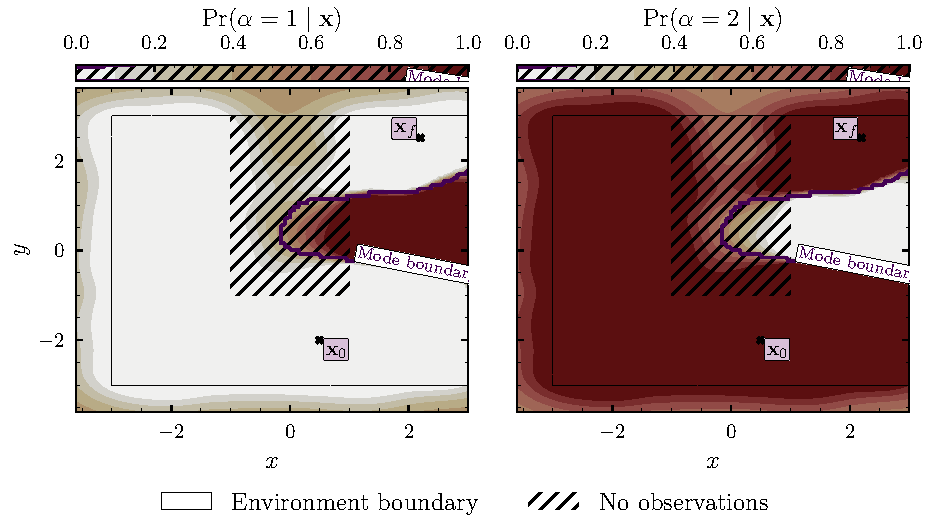
\includegraphics[width=0.98\textwidth]{./images/mode-opt/env/scenario_7/mosvgpe/mixing_probs_no_obs.pdf}
\subcaption{Mixing probabilities}
\label{eq-traj-opt-gating-network-prob-post}
\end{minipage}
\begin{minipage}{1.0\textwidth}
\centering
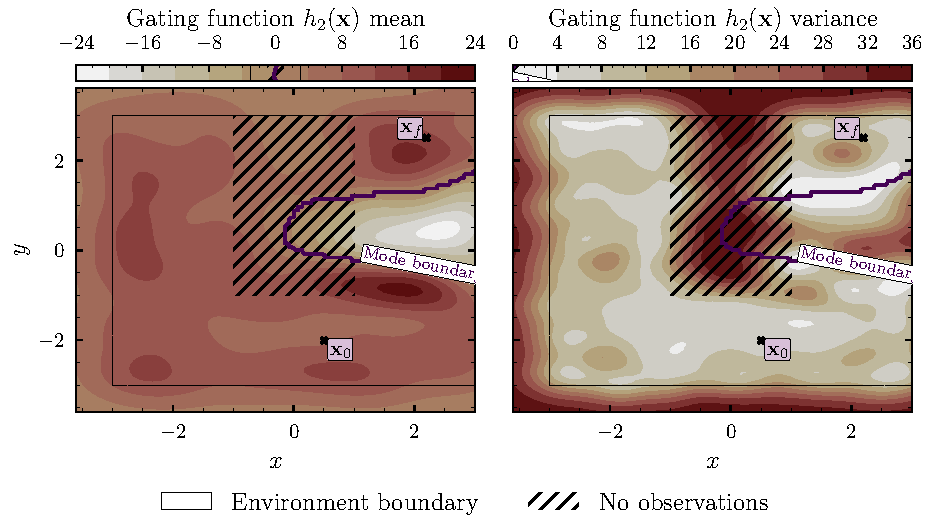
\includegraphics[width=0.98\textwidth]{./images/mode-opt/env/scenario_7/mosvgpe/desired_gating_gp_no_obs.pdf}
\subcaption{Gating function's \acrshort{gp} posterior}
\label{eq-traj-opt-gating-network-gp-post}
\end{minipage}
\caption[\acrshort{mosvgpe}'s gating network posterior after training on simulated quadcopoter data set]{
Visualisation of the gating network posterior after training \acrshort{mosvgpe}
on the state transition data set from the simulated version of the 2D quadcopter environment
in the illustrative example from \cref{illustrative_example}.
(\subref{eq-traj-opt-gating-network-prob-post}) shows the probability mass function over the expert indicator
variable and (\subref{eq-traj-opt-gating-network-gp-post}) shows the gating function's \acrshort{gp}
posterior mean (left) and posterior variance (right).
The start state $\state_0$ and target state $\targetState$ are overlayed along with the mode boundary (purple line)
and the subset of the environment which has not been observed (hashed box).}
\label{fig-traj-opt-gating-network-gp}
\end{figure}
The \acrshort{mosvgpe} model correctly identifies the underlying dynamics modes and infers informative
latent spaces that can be used to encode mode remaining behaviour.
\cref{fig-traj-opt-gating-network-gp} shows the gating network posterior after training
\acrshort{mosvgpe} on the historical data set of state transitions from the illustrative quadcopter
example in \cref{illustrative_example}.
The work in this chapter is based on the observation that
Goals 1 and 2 can be encoded as finding length minimising trajectories on the manifold parameterised by the
desired mode's gating function, shown in the left-hand plot of \cref{eq-traj-opt-gating-network-gp-post}.
Intuitively, the length of a trajectory from \(\mathbf{x}_0\) to \(\mathbf{x}_f\) on the
manifold given by the desired mode's gating function,
increases when it passes over the contours; analogous to climbing a hill.
Given appropriate scaling of the gating function, shortest trajectories between two locations are
those that attempt to follow the contours, and as a result,
remain in a single mode by not climbing up or down any hills.
This section will review the relevant concepts from Riemannian geometry and show how they can be used
to encode Goals 1 and 2.
\cref{sec-prob-geo} then extends these concepts to probabilistic geometries to encode Goal 3.

\newline
\textbf{Lengths in Euclidean spaces}
The \(l^2\) norm (Euclidean norm) provides an intuitive notion for the length of a
vector \(\manifoldInput \in \manifoldDomain \subseteq \R^{\manifoldDomainDim}\) in a Euclidean space.
A continuous-time trajectory is denoted \(\trajectory: [t_0, t_f] \rightarrow \manifoldDomain\).
Note that this has overloaded the discrete-time trajectory notation.
Under the \(l^2\) norm, the length of a trajectory \(\trajectory\) is given by,
\begin{align} \label{eq-euclidean-length}
\text{Length}\left(\trajectory\right)
&= \int_{t_0}^{t_f}\left\|\dot{\manifoldInput}(t)\right\|_2 \mathrm{d}t,
\end{align}
where Newton's notation has been used to denote differentiation with respect to time \(t\).
As a norm can be expressed for any space endowed with an inner product, it is possible to
calculate lengths of trajectories on manifolds endowed with an inner product.

\newline
\begin{myquote}
\textbf{Riemannian manifolds}
In this thesis it suffices to consider manifolds $\manifold$ defined by a mapping,
%#+BEGIN_EXPORT latex
\begin{equation} \label{eq-manifold-function}
\manifoldFunction : \manifoldDomain \rightarrow \manifoldCodomain,
\end{equation}
%#+END_EXPORT
where $\manifoldDomain$ and $\manifoldCodomain$ are open subsets of Euclidean spaces.
The manifold $\manifold$ is given by $\manifold = \manifoldFunction(\manifoldDomain)$ and is said to
be immersed in the ambient space $\manifoldCodomain$.
The dimensionality of the surface is denoted $\manifoldDomainDim = \text{dim}(\manifoldDomain)$
whilst $\manifoldCodomainDim = \text{dim}(\manifoldCodomain)$ denotes the dimensionality of the ambient space.
Riemannian manifolds can intuitively be seen as $\manifoldCodomainDim\text{-dimensional}$
curved surfaces with a smoothly
varying positive-definite inner product, governed by the Riemannian metric $\metricTensor$ \citep{carmoRiemannian1992}.
\begin{definition}[Riemannian Metric]
A Riemannian metric $\metricTensor$,
on a manifold $\manifold$, is a smooth function
$\metricTensor : \manifoldDomain \rightarrow \R^{\manifoldDomainDim \times \manifoldDomainDim}$
that assigns a symmetric positive definite matrix to any point in $\manifoldDomain$.
%A Riemannian metric $\metricTensor$ on a
%manifold $\manifold$ is a symmetric and positive definite matrix which defines
%a smoothly varying inner product
%$\langle \dot{\mathbf{x}}_a, \dot{\mathbf{x}}_b \rangle_{\mathbf{x}} = \dot{\mathbf{x}}_a^T \mathbf{G}(\mathbf{x}) \dot{\mathbf{x}}_b$
%in the tangent space $T_{\mathbf{x}}\manifold$, for each point $\mathbf{x} \in \manifold$ and
%$\dot{\mathbf{x}}_a, \dot{\mathbf{x}}_b \in T_{\mathbf{x}}\manifold$.
\end{definition}
Intuitively, the metric forms a local inner product in $\manifoldDomain$ that informs how to measure lengths
on the manifold $\manifold$, locally in $\manifoldDomain$.
This is indicated in \cref{eq-manifold-norm}.
Riemannian manifolds locally resemble Euclidean spaces and have
globally defined differentiable structure.
\end{myquote}
\newline

\textbf{Lengths on Riemannian manifolds}
The length of a trajectory \(\trajectory\) on a manifold \(\manifold\), can be calculated
by mapping it through the function \(\manifoldFunction\) and
using \cref{eq-euclidean-length},
\begin{align} \label{eq-manifold-length}
\text{Length}\left(\manifoldFunction(\trajectory)\right)
&= \int_{t_0}^{t_f}\left\|\dot{\manifoldFunction}(\manifoldInput(t))\right\|_2 \mathrm{d}t.
\end{align}
Applying the chain-rule allows \cref{eq-manifold-length} to be expressed in terms of the Jacobian and the
velocity,
\begin{align} \label{eq-manifold-length-chain}
\text{Length}\left(\manifoldFunction(\trajectory)\right)
&= \int_{t_0}^{t_f}\left\|\jacobian \dot{\manifoldInput}(t)\right\|_2 \mathrm{d}t, \\
\jacobian &= \frac{\partial \manifoldFunction}{\partial \manifoldInput(t)} \in \R^{1 \times \manifoldDomainDim}.
\end{align}
This implies that the length of a trajectory on the manifold \(\manifold\),
can be calculated in the input space \(\manifoldDomain\),
using a locally defined norm,
\begin{align} \label{eq-manifold-norm}
\left\|\jacobian \dot{\manifoldInput}(t)\right\|_2
&= \sqrt{ \left( \jacobian \dot{\manifoldInput}(t) \right)^T
\left( \jacobian \dot{\manifoldInput}(t)} \right) \nonumber \\
&= \sqrt{\dot{\mathbf{x}}^T(t) \metricTensor_{\mathbf{x}_t} \dot{\manifoldInput}(t)}
\defeq \left\|\dot{\manifoldInput}(t)\right\|_{\metricTensor_{\manifoldInput_t}},
%= \left\|\dot{\mathbf{x}}(t)\right\|_{\mathbf{G}(\mathbf{x}(t))}.
\end{align}
where \(\metricTensor_{\mathbf{x}_t} = \jacobian^T \jacobian\)
is a symmetric positive definite matrix
(akin to a local Mahalanobis distance measure), known as the natural Riemannian metric.
The length of a trajectory on a manifold \(\manifold\), endowed with the metric \(\metricTensor\),
can then be calculated with,
\begin{align} \label{eq-manifold-length-G}
\text{Length}(\manifoldFunction(\trajectory))
&= \int_{t_0}^{t_f}\left\|\dot{\manifoldInput}(t)\right\|_{\metricTensor_{\mathbf{x}_t}} \mathrm{d}t.
\end{align}

\cref{fig-traj-opt-gating-network-gp} shows the \acrshort{gp} posterior over the desired mode's gating function,
\(\desiredGatingFunction : \stateDomain \rightarrow \gatingCodomain\).
Consider finding
length minimising trajectories on the manifold \(\desiredManifold=\desiredGatingFunction(\gatingDomain)\)
associated with the desired mode's gating function, where the metric is given by,
\begin{align} \label{eq-desired-metric-tensor}
\desiredMetricTensor &= \desiredJacobian^T \desiredJacobian, \\
\desiredJacobian &= \frac{\partial \desiredGatingFunction}{\partial \manifoldInput(t)} \in \R^{1 \times \GatingDim}.
\end{align}
These trajectories will attempt to remain in the desired dynamics mode \(\desiredMode\), encoding Goals 1 and 2.
However, length minimising trajectories subject to this metric do not encode Goal 3.
That is, they will not avoid regions of the learned dynamics, which cannot be predicted confidently due to
high \emph{epistemic uncertainty}.
Goal 3 can be encoded by observing that the metric tensor is actually a random variable and extending the concepts
of length minimising trajectories to probabilistic manifolds.

\subsubsection{Probabilistic Geometries \label{sec-prob-geo}}
\label{sec:orge4e9846}
\newline

Following \cite{tosiMetrics2014} we formulate a metric tensor that captures the variance in the manifold
via a probability distribution.
First note that as the differential operator is linear, the derivative of a \acrshort{gp} is also a \acrshort{gp},
assuming that the mean and covariance functions are differentiable.
\begin{assumption}[Differentiable Gaussian Process] \label{}
Let $\mu : \stateDomain \rightarrow \R$ and $k: \stateDomain \times \stateDomain \rightarrow \R$
denote the mean and covariance functions associated with a Gaussian process.
The Gaussian process is differentiable iff
$\exists \frac{\partial \mu(\state)}{\partial \state}, \frac{\partial^2 k(\state, \state')}{\partial \state \partial \state'} \quad \forall \state, \state' \in \stateDomain$.
\end{assumption}

%\todo{should there be minus mean function in jac?}
\begin{myquote}
\textbf{Gaussian Process Jacobian}
As the differential operator is linear, a function $\manifoldFunction: \gatingDomain \rightarrow  \R$ distributed as a \acrshort{gp},
\begin{align} \label{eq-jacobian-gp-random-var}
\manifoldFunction(\cdot) \sim \mathcal{GP}\left(\mu(\cdot), k(\cdot, \cdot)\right),
\end{align}
%\begin{align} \label{eq-jacobian-gp-random-var}
%\manifoldFunction(\allInput) \sim \mathcal{GP}\left(\mu(\allInput), k(\allInput, \allInput)\right),
%\end{align}
where $\mu$ and $k$ represent the mean and covariance functions,
is jointly Gaussian with its Jacobian
at a new input location $\testInput \in \R^{1 \times \GatingDim}$,
\begin{align} \label{eq-jacobian-random-var} \testJac = \Jac(\testInput) = \frac{\partial \manifoldFunction}{ \partial \testInput} \in \R^{\GatingDim},
\end{align}
assuming that the mean and covariance functions are differentiable.
As such, the conditional distribution over the Jacobian
$\testJac$ can be obtained using the properties of multivariate normals
and is given by,
%\begin{align} \label{eq-predictive-jacobian-dist}
%\Jac(\cdot)
%&\sim \mathcal{GP}\left(
%\underbrace{\partial \mu(\cdot) + \jacManifoldKerneldN \manifoldKernelNN^{-1} \manifoldFunction(\allInput)}_{\muJac},
%\underbrace{\hessManifoldKerneldd - \jacManifoldKerneldN \manifoldKernelNN^{-1} \jacManifoldKernelNd}_{\covJac}
%\right),
%\end{align}
\begin{align} \label{eq-predictive-jacobian-dist}
\testJac
&\sim \mathcal{N}\left(
\underbrace{\frac{\partial \mu}{\partial \testInput} + \jacManifoldKernelsN \manifoldKernelNN^{-1} \manifoldFunction(\allInput)}_{\muJac},
\underbrace{\hessManifoldKernel - \jacManifoldKernelsN \manifoldKernelNN^{-1} \jacManifoldKernelNs}_{\covJac}
\right),
\end{align}
%\begin{align} \label{eq-predictive-jacobian-dist}
%p\left(\testJac | \manifoldFunction(\allInput), \testInput, \allInput \right)
%&= \mathcal{N}\left(\testJac \mid \muJac, \covJac \right) \\
%\muJac &= \frac{\partial \mu}{\partial \testInput} + \jacManifoldKernelsM \manifoldKernelNN^{-1}
%\left(\manifoldFunction(\allInput) - \manifoldMeanFunc(\allInput) \right) \\
%\muJac &= \frac{\partial \mu}{\partial \testInput} + \jacManifoldKernelsM \manifoldKernelNN^{-1}
%\manifoldFunction(\allInput) \\
%\covJac &= \hessManifoldKernel - \jacManifoldKernelsN \manifoldKernelNN^{-1} \jacManifoldKernelNs
%\end{align}
where the covariance matrices are given by,
\begin{align} \label{eq}
\manifoldKernelNN &= k\left( \allInput, \allInput \right) \in \R^{\NumData \times \NumData} \\
\jacManifoldKernelsN&= \frac{\partial k\left(\testInput, \allInput\right)}{\partial \testInput} \in \R^{\GatingDim \times \NumData} \\
\hessManifoldKernel &= \frac{\partial^2 k\left(\testInput, \testInput \right)}{\partial \testInput \partial \testInput} \in \R^{\GatingDim \times \GatingDim}.
\end{align}
\cref{eq-predictive-jacobian-dist} is a $\GatingDim\text{-dimensional}$ multivariate normal distribution.
\end{myquote}

Therefore, the metric tensor \(\desiredMetricTensor\) in \cref{eq-desired-metric-tensor} is the outer product of
two normally distributed random variables.
As such, the metric tensor \(\desiredMetricTensor\) is also a random variable, following
a non-central Wishart distribution \citep{andersonNonCentral1946},
\begin{align} \label{eq-metric-dist}
  \desiredMetricTensor \sim
  \mathcal{W}_{\GatingDim}\left(P, \covJac, \mathbb{E}\left[\Jac^{T}\right] \mathbb{E}[\Jac]\right),
\end{align}
where \(P\) is the number of degrees of freedom (always one in our case) and
\(\E\left[\desiredJacobian\right]\) and \(\covJac\) are the mean and covariance matrices
associated with the \acrshort{gp} over the Jacobian.
The expected value of the metric tensor in \cref{eq-metric-dist} is given by,
\begin{align} \label{eq-expected-metric}
  \E[\desiredMetricTensor] = \E[\mathbf{J}^T] \E[\mathbf{J}] + \covJac.
\end{align}
Importantly, this expected metric tensor includes a covariance term \(\covJac\),
which implies that lengths on the manifold calculated under this expected metric will
increase in areas of high covariance.
This is a desirable behaviour because it encourages length minimising trajectories
to avoid regions of the learned dynamics with high \emph{epistemic uncertainty},
encoding Goal 3.
To aid with user control, the metric tensor in \cref{eq-expected-metric} is modified with
a weighting parameter \(\lambda\) that enables the relevance of the covariance term to be adjusted,
\begin{align} \label{eq-expected-metric-weighting}
  \tilde{\mathbf{G}} = \E[\mathbf{J}^T] \E[\mathbf{J}] + \lambda \mathbf{\Sigma}_J.
\end{align}
Setting \(\lambda\) to be small should find trajectories that prioritise staying in the desired mode,
whereas selecting a large \(\lambda\) should find trajectories that prioritise avoiding regions
of the dynamics with high \emph{epistemic uncertainty}.

\subsubsection{Extension to Sparse Variational Gaussian Processes}
\label{sec:org79bd84d}
The model in Chapter \ref{chap-dynamics} is built upon sparse \acrshort{gp} approximations,
so the Jacobian in \cref{eq-predictive-jacobian-dist} must be extended for such approximations.
\begin{myquote}
\textbf{Sparse Gaussian Process Jacobian}
To obtain the distribution over the Jacobian
in the sparse variational Gaussian process setting, we first condition on the inducing variables
$\manifoldInducingOutput  \in \R^{\NumInducing \times 1}$,
%\begin{equation} \label{eq-}
%\manifoldInducingOutput \sim \mathcal{GP}\left(\mu(\manifoldInducingInput),
%k(\manifoldInducingInput, \manifoldInducingInput)\right)
%\end{equation}
\begin{equation} \label{eq-}
\testJac \mid \manifoldInducingOutput \sim \mathcal{N}\left(
\frac{\partial \mu}{\partial \testInput} + \jacManifoldKernelsM \manifoldKernelMM^{-1}
\manifoldInducingOutput,
\hessManifoldKernel - \jacManifoldKernelsM \manifoldKernelMM^{-1}
\jacManifoldKernelMs \right).
\end{equation}
where the inducing variables' density is from the prior in \cref{eq-jacobian-gp-random-var},
so the covariance matrices are given by,
\begin{align} \label{eq-}
\manifoldKernelMM &= k\left( \manifoldInducingInput, \manifoldInducingInput \right) \in \R^{\NumInducing \times \NumInducing} \\
\jacManifoldKernelsM&= \frac{\partial k\left(\testInput, \manifoldInducingInput \right)}{\partial \testInput} \in \R^{\GatingDim \times \NumInducing}.
\end{align}
The distribution over the Jacobian is then obtained by marginalising the inducing variables
with respect to their variational density,
\begin{equation} \label{eq-}
q(\manifoldInducingOutput) = \mathcal{N}\left(\manifoldInducingOutput \mid \manifoldInducingOutputMean, \manifoldInducingOutputCov \right).
\end{equation}
The distribution over the Jacobian is then obtained via a Gaussian convolution,
\begin{align}
%q(\testJac \mid \testInput)
\testJac &\sim \mathcal{N}\left(
\underbrace{\frac{\partial \mu}{\partial \testInput} + \jacManifoldKernelsM \manifoldKernelMM^{-1}
\manifoldInducingOutputMean}_{\muJac},
\underbrace{\hessManifoldKernel - \jacManifoldKernelsM \manifoldKernelMM^{-1}
\left( \manifoldKernelMM - \manifoldInducingOutputCov \right) \manifoldKernelMM^{-1} \jacManifoldKernelMs}_{\covJac}
\right).
\end{align}
%The distribution over the Jacobian is approximated as follows,
%\begin{align}
%p(\testJac \mid \testInput, \allOutput, \allInput) &=
%\int \int p(\testJac \mid \testInput, \manifoldFunction(\allInput), \manifoldInducingOutput)
%p(\manifoldFunction(\allInput), \manifoldInducingOutput \mid \allOutput, \allInput)
%\text{d} \manifoldFunction(\allInput) \text{d} \manifoldInducingOutput \nonumber \\
%&\approx \int \int p(\testJac \mid \testInput, \manifoldFunction(\allInput), \manifoldInducingOutput)
%p(\manifoldFunction(\allInput) \mid \manifoldInducingOutput) \manifoldInducingVariational
%\text{d} \manifoldFunction(\allInput) \text{d} \manifoldInducingOutput \nonumber \\
%&= \int  p(\testJac \mid \testInput, \manifoldInducingOutput)
%\manifoldInducingVariational
%\text{d} \manifoldInducingOutput
%\coloneqq q(\testJac \mid \testInput)
%\end{align}
%where the mean and covariance are given by,
%\begin{align} q(\testJac \mid \testInput) &= \mathcal{GP}\left(\muJac, \covJac \right) \\
%\muJac &= \frac{\partial \mu}{\partial \testInput} + \jacManifoldKernelsM \manifoldKernelMM^{-1}
%\left( \manifoldInducingOutputMean - \manifoldMeanFunc(\allInput) \right), \\
%\covJac &= \hessManifoldKernel - \jacManifoldKernelsM \manifoldKernelMM^{-1}
%\left( \manifoldKernelMM - \manifoldInducingOutputCov \right) \manifoldKernelMM^{-1} \jacManifoldKernelMs \right).
%\end{align}
\end{myquote}

\subsection{\acrfull{ig} \label{sec-traj-opt-collocation}}
\label{sec:org8b3b85f}
This section presents a trajectory optimisation algorithm that exploits the fact that
length minimising trajectories on the manifold endowed with the expected metric from \cref{eq-expected-metric},
encodes all of the goals.
As shortest lengths on a manifold are known as geodesics, we refer to them as geodesic trajectories.
The algorithm presented in this section
exploits a classic result of Riemannian geometry, that geodesic trajectories are solutions
to a 2\textsuperscript{nd} order \acrshort{ode}, known as the geodesic \acrshort{ode} \(f_G\).
As solutions to this \acrshort{ode} encode the necessary conditions for finding length minimising trajectories,
the method presented in this section resembles an indirect optimal control method.

\begin{myquote}
\textbf{Geodesics}
Given the method for calculating lengths on Riemannian manifolds in \cref{eq-manifold-length-G},
the notion of a shortest trajectory, or geodesic trajectory, is defined as follows,
\begin{definition}[Geodesic]
Given two points $\manifoldInput_0, \manifoldInput_f \in
\manifold = \manifoldFunction(\manifoldDomain)$, a Geodesic is a length minimising trajectory (curve)
$\trajectory_g$ connecting the points, such that,
\begin{subequations} \label{eq-geodesic}
\begin{align}
  \trajectory_{g} =\arg &\min_{\trajectory} \operatorname{Length}(\manifoldFunction(\trajectory)) \\
\text{s.t.} \quad  \manifoldInput(t_0)&=\manifoldInput_{0} \\
  \manifoldInput(t_f)&=\manifoldInput_{f}.
\end{align}
\end{subequations}
\end{definition}
\end{myquote}
\textbf{Geodesic \acrshort{ode}} An important observation from \cite{carmoRiemannian1992}, is that geodesics
satisfy a continuous-time \(2^{\text{nd}}\) order \acrshort{ode}, given by,
\begin{align} \label{eq-2ode}
 \ddot{\manifoldInput}(t)
&= \geodesicFunction(t, \manifoldInput, \dot{\manifoldInput}) \nonumber \\
&=-\frac{1}{2} \metricTensor^{-1}(\manifoldInput(t))\left[
\frac{\partial \operatorname{vec}[\metricTensor(\manifoldInput(t))]}{\partial \manifoldInput(t)}
\right]^{T}\left(\dot{\manifoldInput}(t) \otimes \dot{\manifoldInput}(t)\right),
\end{align}
where \(\operatorname{vec}[\metricTensor(\manifoldInput(t)])\) stacks the columns of \(\metricTensor(\manifoldInput(t))\)
and \(\otimes\) denotes the Kronecker product.
The implication of \cref{eq-geodesic,eq-2ode}, is that trajectories that are solutions
to the \(2^{\text{nd}}\) order \acrshort{ode} in \cref{eq-2ode}, implicitly minimise their length on the manifold,
i.e. the objective in \cref{eq-manifold-length-G}.
Given this observation, computing geodesics involves finding a solution to \cref{eq-2ode}
with \(\manifoldInput(t_0) = \manifoldInput_0\) and \(\manifoldInput(t_f) = \manifoldInput_f\).
This is a boundary value problem (BVP) with a smooth solution so it can be solved using
any BVP solver, e.g. (multiple) shooting or collocation methods.
\subsubsection{Implicit Trajectory Optimisation}
\label{sec:org8c2c676}
Solving the 2\textsuperscript{nd} order \acrshort{ode} in \cref{eq-2ode} with the expected metric from \cref{eq-expected-metric-weighting},
is equivalent to solving our trajectory optimisation problem subject to the same boundary conditions.
This resembles an indirect optimal control method as it is based on an observation that the
necessary conditions for optimality are encoded via the geodesic \acrshort{ode}.
However, it is worth noting that solutions to the geodesic \acrshort{ode} are not guaranteed to satisfy the
dynamics constraints.


\textbf{Collocation}
Since neither \(\dot{\mathbf{x}}(t_0)\) nor \(\dot{\mathbf{x}}(t_f)\) are known, \cref{eq-2ode} cannot
be solved with simple forward or backward integration.
Instead, the problem is transcribed using collocation.
Collocation methods are used to transcribe continuous-time trajectory optimisation problems into
nonlinear programs, i.e. constrained parameter optimisations \citep{kellyIntroduction2017,fahrooDirect2000}.
The expected metric in \cref{eq-expected-metric} is substituted into \cref{eq-2ode} and solved via collocation.
This work implements a Hermite-Simpson collocation method.
It parameterises the state trajectory using cubic polynomials and the dynamics equations (the geodesic \acrshort{ode} in this case)
are imposed as constraints at a set of collocation points.
The trajectory \([t_0, t_f]\) is discretised into \(I\) intervals where the collocation points
are the mid points of the discretisation intervals.
The collocation states
\(\bar{\stateCol} = \{\stateCol_{i+\frac{1}{2}}\}_{i=0}^{I-1}\)
are obtained by interpolating the polynomials.
The derivative of the collocation states w.r.t. time
\(\{\dot{\stateCol}_{i+\frac{1}{2}}, \ddot{\stateCol}_{i+\frac{1}{2}}\}_{i=0}^{I-1}\)
are obtained algebraically via the polynomials.
The collocation constraints then enforce
the second derivative of the collocation states interpolated by the polynomials \(\{\ddot{\stateCol}_{i+\frac{1}{2}} \}_{i=0}^{I-1}\),
to equal the geodesic \acrshort{ode} \(f_G\) at the collocation points.
This is achieved through the collocation defects,
\begin{align} \label{eq-defect}
\Delta\ddot{\stateCol}_{i+\frac{1}{2}} &= \ddot{\stateCol}_{i+\frac{1}{2}} - f_G(t_{i+\frac{1}{2}}, \stateCol_{i+\frac{1}{2}}, \dot{\stateCol}_{i+\frac{1}{2}}) = 0 \quad \forall i \in  \{ 0, \ldots, I-1\},
\end{align}
where \(\ddot{\stateCol}_{i+\frac{1}{2}}, \dot{\stateCol}_{i+\frac{1}{2}}, \stateCol_{i+\frac{1}{2}}\)
are obtained by interpolating between \(i\) and \(i+1\).
\cref{eq-defect} defines a set of constraints that ensure trajectories are solutions
to the geodesic \acrshort{ode} \(f_G\).
The nonlinear program that this method solves is given by,
\begin{subequations} \label{eq-collocation-problem}
\begin{align}
%\min_{\stateCol(t), \dot{\stateCol}(t)}& \int_{t_0}^{t_f}
%\costFunc(\stateCol(\timeInd), \dot{\stateCol}(\timeInd)) \text{d}t \\
\min_{\stateCol_0 \ldots \stateCol_I, \dot{\stateCol}_0 \ldots \dot{\stateCol}_I}& \sum_{i=0}^{I-1}
\costFunc(\stateCol_i, \dot{\stateCol}_i ) \\
\text{s.t.} \quad
\Delta\ddot{\stateCol}_{i+\frac{1}{2}} &= 0 \quad \forall i \in \{0, \ldots, I-1\} \\
\stateCol_0 &= \state_0 \\
\stateCol_I &= \targetState.
\end{align}
\end{subequations}
Notice that no integrals need to be computed as all of the functions are algebraic operations.
In practice, a quadratic cost function is used to regularise the state derivative \(\dot{\stateCol}\),
\begin{align} \label{eq-quadratic-cost-state-derivative}
\costFunc(\stateCol_i, \dot{\stateCol}_i)
&= \dot{\stateCol}_i^T \controlCostMatrix \dot{\stateCol}_i
= \left\| \dot{\stateCol}_i \right\|_{\controlCostMatrix},
\end{align}
where \(\controlCostMatrix\) is a user-defined, real symmetric positive definite weight matrix.
It is solved using \acrfull{slsqp} in SciPy \citep{2020SciPy-NMeth}.

\textbf{Latent variable controls}
This nonlinear program returns a collocation state trajectory \(\bar{\stateCol}\) which parameterises a
continuous-time state trajectory (via the polynomials).
However, it does not return the control trajectory.
The control trajectory is recovered from the state trajectory by performing inference in the
probabilistic dynamics model.
In order to do this, the state trajectory is first discretised.
In practice, using the collocation states as the discretised state trajectory worked well, i.e.
\(\stateTraj = \{\state_{\timeInd}\}_{\timeInd=0}^{I} = \{\stateCol_{i}\}_{i=0}^{I}\).
The state difference outputs \(\stateDiffTraj = \{\stateDiff_{\timeInd}\}_{\timeInd=1}^{\TimeInd}\) are
calculated from the state trajectory \(\stateTraj\).
The control trajectory \(\controlTraj\) is then inferred from the state trajectory by extending
the \acrshort{elbo} for the desired mode's \acrshort{svgp} expert with latent variable inputs.
Following \cite{hensmanGaussian2013}, the \acrshort{elbo} for a single \acrshort{svgp} expert is given by,
\begin{align}
\log p(\stateDiffTraj \mid \stateTraj, \controlTraj) \geq
\E_{q(\mode{\latentFunc}(\stateTraj, \controlTraj))} \left[ \nonumber
&\log p(\stateDiffTraj \mid \mode{\latentFunc}(\stateTraj, \controlTraj)) \right] \\
&- \text{KL}\left(q(\mode{\latentFunc}(\expertInducingInput)) \mid p(\mode{\latentFunc}(\expertInducingInput))) \right)
\coloneqq \mathcal{L}_{\text{SVGP}},
\end{align}
where the variational posterior is given by
\(q(\mode{\latentFunc}(\stateTraj, \controlTraj)) &= \int p(\mode{\latentFunc}(\stateTraj, \controlTraj) \mid \mode{\latentFunc}(\expertInducingInput)) q(\mode{\latentFunc}(\expertInducingInput)) \text{d} \mode{\latentFunc}(\expertInducingInput)\).
The control inputs \(\controlTraj\) are recovered by treating them as latent variables and extending the lower bound to,
\begin{align}  \label{eq-control-elbo-svgp}
\log p(\stateDiffTraj \mid \stateTraj) &= \log \int p(\stateDiffTraj \mid \stateTraj, \controlTraj) p(\controlTraj) \text{d}\controlTraj \\
&\geq \E_{q(\controlTraj)} \left[ \mathcal{L}_{\text{SVGP}} + \log p(\controlTraj) - \log q(\controlTraj) \right],
\label{eq-control-elbo}
\end{align}
where each time step of the latent control trajectory is assumed to be normally distributed,
\begin{align}
p(\controlTraj) = \prod_{\timeInd=0}^{\TimeInd-1} \mathcal{N}(\control_{\timeInd} \mid \mathbf{0}, \mathbf{I}),
\end{align}
and its variational posterior is given by,
\begin{align}
q(\controlTraj) = \prod_{\timeInd=0}^{\TimeInd-1} \mathcal{N}(\control_{\timeInd} \mid \mathbf{m}_{\timeInd}, \mathbf{S}_{\timeInd}).
\end{align}
The posterior over the latent control trajectory \(q(\controlTraj) \approx p(\controlTraj \mid \stateTraj, \stateDiffTraj)\)
is obtained by finding the variational parameters
\(\{\mathbf{m}_{\timeInd}, \mathbf{S}_{\timeInd}\}_{\timeInd=0}^{\TimeInd-1}\) that maximise the \acrshort{elbo} in
\cref{eq-control-elbo}.

Although this method provides an elegant solution to finding trajectories that satisfy Goals 1, 2 and 3,
it is not without its limitations.
First of all, this approach does not necessarily find trajectories that satisfy the dynamics constraints,
as it projects the problem onto the geodesic \acrshort{ode}.
\begin{remark}
Dynamics constraints are not guaranteed to be satisfied.
\end{remark}
Secondly, it does not consider the full distribution over state-control trajectories.
Without the inclusion of the full probabilistic dynamics model, it is impossible
to consider the full distribution over state-control trajectories.
Although propagating uncertainty through a single dynamics \acrshort{gp} is straightforward,
handling the collocation constraints is not.
This is because the geodesic \acrshort{ode} will become a \acrfull{sde}.
\begin{remark}
Ignores much of the stochasticity inherent in the problem.
\end{remark}
\subsection{\acrfull{dre} \label{sec-traj-opt-energy}}
\label{sec:org7b8ed52}
This section details a direct optimal control approach which embeds the mode remaining behaviour directly into the
\acrfull{soc} problem, via a geometric objective function.
In contrast to the previous approach, this method:
\begin{enumerate}
\item enforces the dynamics constraints,
\item principally handles the uncertainty associated with the dynamics.
\end{enumerate}
This approach is a shooting method that enforces the dynamics constraints through simulation, i.e.
the state trajectory is enforced to match the integral of the dynamics with respect to time.

Similar to the previous approach, this method builds on the observation that
length minimising trajectories on the Riemannian manifold \(\manifold\),
associated with the desired mode's gating function \(\desiredGatingFunction\), encodes the goals.
Further to this, this method exploits the fact that length minimising trajectories on a Riemannian manifold \(\manifold\),
are also energy minimising trajectories \citep{carmoRiemannian1992}.
As such, mode remaining behaviour can be encoded by solving,
\begin{subequations} \label{eq-mode-soc-problem-geometry}
\begin{align}
%\min_{\controlTraj} \E_{\state_{\timeInd+1} \sim p(\state_{\timeInd+1} \mid \state_\timeInd, \control_\timeInd)}
\min_{\controlTraj} &J_{\pi}(\state_0) \\
\text{s.t. } &\state_{\timeInd+1} \sim p(\state_{\timeInd+1} \mid \state_\timeInd, \control_\timeInd) \quad &\forall \timeInd \in \{0, \ldots, \TimeInd-1\}  \\
&\control_{\timeInd} \in \controlDomain \quad &\forall \timeInd \in \{0, \ldots, \TimeInd-1\} \\
&\state_0 =\state_0
\end{align}
\end{subequations}
with an objective function that minimises the Riemannian energy,
\begin{align} \label{eq-mode-soc-problem-geometry-cost}
%\min_{\controlTraj} \E_{\state_{\timeInd+1} \sim p(\state_{\timeInd+1} \mid \state_\timeInd, \control_\timeInd)}
J_{\pi}(\state) = \E \Bigg[
\underbrace{\text{Energy}(\manifoldFunction(\stateTraj))}_{\text{Riemannian energy}} &+
\underbrace{(\terminalState - \targetState)^T \terminalStateCostMatrix (\terminalState - \targetState)}_{\text{terminal cost}}
+ \sum_{\timeInd=0}^{\TimeInd-1}
\underbrace{\control_{\timeInd}^T \controlCostMatrix \control_{\timeInd}}_{\text{control cost}}
\mid \state_0 = \state\Bigg],
\end{align}
where \(\terminalStateCostMatrix\) and \(\controlCostMatrix\) are user-defined,
real, symmetric, positive semi-definite and positive definite matrices respectively.
The energy of a trajectory on a Riemannian manifold, endowed with the metric \(\metricTensor\), is given by,
\begin{align} \label{eq-trajectory-energy}
\text{Energy}(\manifoldFunction(\trajectory)) = \sum_{\timeInd=1}^{\TimeInd}
\stateDiff_{\timeInd}^T \metricTensor_{\state_{\timeInd}} \stateDiff_{\timeInd},
\end{align}
where \(\stateDiff_{\timeInd} = \state_{\timeInd} - \state_{\timeInd-1}\) is the state difference.
The mode remaining behaviour and the terminal state boundary condition are encoded via the objective function.
\begin{remark} \label{}
In contrast to the collocation solver in \cref{sec-traj-opt-collocation},
the terminal state boundary condition is encoded via the cost function, instead of being enforced by the solver.
\end{remark}
This may seem like an easy optimisation problem,
however, calculating the expected cost in \cref{eq-mode-soc-problem-geometry-cost} is not straightforward.
Given a starting state \(\state_0\) and a control trajectory \(\controlTraj\),
the expectation in \cref{eq-mode-soc-problem-geometry-cost} is taken with respect to the joint
state-metric distribution over a trajectory, \(p(\stateTraj, \metricTensorTraj, \mid \state_0, \controlTraj)\).
Calculating this expectation is difficult as multi-step predictions in the \acrshort{mosvgpe} dynamics model
cannot be calculated in closed form.

This work adopts a two-stage approximation to obtain a closed-form expression for the expected cost.
First, multi-step dynamics predictions are approximated to obtain normally distributed states at
each time step.
Given normally distributed states, calculating the expected terminal and control cost terms in
\cref{eq-mode-soc-problem-geometry-cost} is straightforward.
However, the expected Riemannian energy in \cref{eq-mode-soc-problem-geometry-cost} has no closed-form expression,
due to the dependence of metric \(\metricTensor\) on the state.
The second stage approximates the calculation of the expected Riemannian energy under normally distributed states.
\subsubsection{Approximate Inference for Dynamics Predictions \label{sec-dynamics-predictions}}
\label{sec:orga6e812f}
\renewcommand{\singleInput}{\ensuremath{\state_\timeInd, \control_\timeInd}}
\renewcommand{\singleInput}{\ensuremath{\hat{\state}_\timeInd}}
\renewcommand{\singleOutput}{\ensuremath{\Delta\state_{\timeInd+1}}}

\newcommand{\desiredExpertKernel}{\ensuremath{k_{\desiredMode}}}
\newcommand{\desiredExpertInducingInput}{\ensuremath{\bm\zeta_{\desiredMode}}}

\newcommand{\expertInducingPrior}{\ensuremath{p(\expertInducingOutput)}}
\newcommand{\expertsInducingPrior}{\ensuremath{p(\expertsInducingOutput)}}
%\newcommand{\expertInducingVariational}{\ensuremath{q(\mode{\latentFunc}(\expertInducingInput))}}
\newcommand{\expertInducingVariational}{\ensuremath{q(\expertInducingOutput)}}
\newcommand{\expertsInducingVariational}{\ensuremath{q(\expertsInducingOutput)}}
\newcommand{\expertsVariational}{\ensuremath{q(\LatentFunc_\numData)}}
%\newcommand{\singleExpertGivenInducing}{\ensuremath{p(\singleOutput \mid \mode{\latentFunc}(\expertInducingInput))}}
\newcommand{\singleExpertGivenInducing}{\ensuremath{p(\singleOutput \mid \expertInducingOutput)}}
%\newcommand{\singleLatentExpertGivenInducing}{\ensuremath{p(\mode{\latentFunc}(\singleInput) \mid \mode{\latentFunc}(\expertInducingInput))}}
\renewcommand{\singleLatentExpertGivenInducing}{\ensuremath{p(\mode{\latentFunc}(\singleInput) \mid \singleInput, \expertInducingOutput)}}

\renewcommand{\expertVariational}{\ensuremath{q(\mode{\latentFunc}(\singleInput) \mid \singleInput)}}

\newcommand{\singleInputMean}{\ensuremath{\hat{\bm\mu}}}
\newcommand{\singleInputCov}{\ensuremath{\hat{\bm\Sigma}}}

Multi-step predictions in the \acrshort{mosvgpe} dynamics model have no closed-form solution  because the state
difference after the first time step is a Gaussian mixture, and
propagating Gaussian mixtures through Gaussian processes has no closed-form solution.
Further to this, constructing approximate closed-form solutions is difficult,
due to the exponential growth in the number of Gaussian components.
\begin{myquote} \label{}
Consider assuming each of the $\ModeInd$ dynamics modes to be independent.
Recursively propagating the Gaussian components associated with the state, through
all of the modes, over a trajectory of length $\TimeInd$, would lead to the final state consisting of
$\ModeInd^{\TimeInd}$ Gaussian components.
\end{myquote}

This work sidesteps this issue and obtains closed-form multi-step predictions
by enforcing that the controlled system remains in the desired dynamics mode.
Multi-step predictions can then be calculated in closed-form by cascading single-step predictions
using the desired dynamics \acrshort{gp}, whose transition density is given by,
\begin{align} \label{eq-single-dynamics-gp}
\transitionDistK
&= \mathcal{N} \left( \latentFunc_{\desiredMode}(\singleInput) \mid
\mathbf{A}_{\desiredMode} \mathbf{m}_{\desiredMode},
\desiredExpertKernel(\singleInput, \singleInput)
+ (\mathbf{S}_{\desiredMode} - \desiredExpertKernel(\desiredExpertInducingInput,\desiredExpertInducingInput))
\mathbf{A}_{\desiredMode}^T
\right)
\end{align}
where
\(\mathbf{A}_{\desiredMode} = \desiredExpertKernel(\singleInput, \desiredExpertInducingInput)\desiredExpertKernel(\desiredExpertInducingInput, \desiredExpertInducingInput)^{-1}\)
and \(\singleInput=(\state_{\timeInd}, \control_{\timeInd})\).
Cascading single-step predictions requires recursively mapping uncertain state-control inputs through
the desired mode's dynamics \acrshort{gp}, i.e. recursively calculating the following integral,
\begin{align} \label{eq-state-unc-prop}
p(\state_{\timeInd+1} \mid \state_0, \control_{0:\timeInd}, \bm\modeVar_{0:\timeInd}=\desiredMode)
&= \int \transitionDistK p(\state_\timeInd \mid \state_{0}, \control_{0:\timeInd-1}, \bm\modeVar_{0:\timeInd-1}=\desiredMode) \text{d}\state_{\timeInd}
\end{align}
with \(p(\state_0) = \delta(\state_0)\).
Approximate closed-form solutions exist for propagating normally distributed states and controls through \acrshort{gp} models
\citep{girardApproximate2004,kussGaussian2006,quinonero-candelaPropagation2003}.
This work exploits the moment-matching approximation from Section 7.2.1 of \cite{kussGaussian2006}.

\textbf{\(\delta-\text{mode remaining}\) chance constraints}
Enforcing the controlled system to remain in the desired dynamics mode simplifies
calculating multi-step predictions and the expected cost in \cref{eq-mode-soc-problem-geometry-cost}.
As the dynamics model is learned from observations, this work relaxes the requirement to ensuring that trajectories
are \(\delta-\text{mode remaining}\) (\cref{def-delta-mode-remaining}).
The conditions to be \(\delta-\text{mode remaining}\) can be enforced with chance constraints,
\begin{align} \label{eq-mode-chance-constraint}
\Pr(\modeVar_{\timeInd} = \desiredMode \mid \state_{0}, \control_{0:\timeInd}, \bm\modeVar_{0:\timeInd-1}=\desiredMode)
\geq 1-\delta \quad \forall \timeInd \in \{0, \ldots, \TimeInd\}.
%\geq \satisfactionProb \quad \forall \timeInd \in \mathbb{Z} \cap [0,\TimeInd].
\end{align}
These constraints enforce the system to remain in the desired dynamics mode with satisfaction probability
\(\satisfactionProb=1-\delta\), at each time step.
As the \acrshort{mosvgpe} model assumes that the mode indicator variable \(\modeVar\)
depends on the state via the gating function, this probability is calculated as follows,
\small
\begin{align} \label{eq-mode-chance-constraint-integral}
\Pr(\modeVar_{\timeInd} = \desiredMode \mid \state_{0}, \control_{0:\timeInd}, \bm\modeVar_{0:\timeInd-1}=\desiredMode) =
&\int \underbrace{\Pr(\modeVar_{\timeInd} = \desiredMode \mid \GatingFunc(\state_{\timeInd}))}_{\text{Bernoulli/softmax likelihood}} \nonumber \\
&\int \underbrace{q(\GatingFunc(\state_{\timeInd}) \mid \state_{\timeInd})}_{\text{approx posterior}}
\underbrace{p(\state_\timeInd \mid \state_{0}, \control_{0:\timeInd-1}, \bm\modeVar_{0:\timeInd-1}=\desiredMode)}_{\text{state dist}}
\text{d} \state_{\timeInd}
\text{d} \GatingFunc(\state_{\timeInd})
\end{align}
\normalsize
where \(q(\GatingFunc(\state_{\timeInd}) \mid \state_{\timeInd})\) is the approximate posterior over the
gating functions from \cref{eq-predictive-gating}.

\subsubsection{Approximate Riemannian Energy}
\label{sec:orgbb96391}
Given this approach for simulating the \acrshort{mosvgpe} dynamics model, the state at each time step is normally distributed.
Unlike the terminal and control cost terms in \cref{eq-mode-soc-problem-geometry-cost}, the expected Riemannian
energy,
\begin{align} \label{eq-trajectory-riemannian-energy}
\E_{\stateTraj, \jacTraj} \left[ \text{Energy}(\stateTraj) \right]
= \sum_{\timeInd=1}^\TimeInd
\E_{\stateDist}\left[ \stateDiff_\timeInd^T
\E_{\Jac_{\state_{\timeInd}} \mid \state_{\timeInd}}\left[ \Jac_{\state_\timeInd} \Jac_{\state_\timeInd}^T \right]
 \stateDiff_\timeInd \right],
\end{align}
has no closed-form expression under normally distributed states.
This is because the metric tensor \(\metricTensor\) depends on the Jacobian, which depends on the state.
However, it is possible to approximate the expected energy to obtain a closed-form expression.

The distribution over the Jacobian when the input location in normally distributed
\(\state_{\timeInd} \sim \mathcal{N}(\stateMean, \stateCov)\) can be calculated in closed-form when using the
Squared Exponential kernel.
However, this work simplifies the problem and calculates the Jacobian at the state mean of each time step
along a trajectory, i.e.
\(\Jac_{\state_{\timeInd}} \approx \frac{\partial \manifoldFunction(\stateMean)}{\partial \stateMean}\).
The distribution over the Jacobian given deterministic inputs can be calculated using \cref{eq-predictive-jacobian-dist}.

Approximating the Jacobian to be independent of the state enables the expected metric tensor to be calculated in
closed-form with \cref{eq-expected-metric-weighting}.
Given this approximation, the Riemannian energy retains a quadratic form, so the expectation with respect to
\(\stateDiff_{\timeInd} \sim \mathcal{N}(\stateDiffMean, \stateDiffCov)\) can be calculated with,
\begin{align} \label{eq-approximate-trajectory-riemannian-energy}
\E \left[ \text{Energy}(\manifoldFunction(\stateTraj)) \right] &\approx
\sum_{\timeInd=1}^\TimeInd
\E_{\stateDiff_{\timeInd}}\left[ \stateDiff_\timeInd^T
\E_{\Jac_{\state_{\timeInd}}}\left[ \metricTensor_{\state_{\timeInd}} \right]
 \stateDiff_\timeInd \right] \nonumber \\
&= \sum_{\timeInd=1}^\TimeInd \stateDiffMean^T (\muJac \muJac^T + \covJac) \stateDiffMean
+ \text{tr}\left(
\left(\muJac \muJac^T + \covJac \right)
\stateDiffCov \right)
\end{align}
\begin{myquote} \label{}
The expected metric tensor encourages trajectories to 1) follow contours on the desired mode's gating function,
encoding Goal 2, i.e. mode remaining behaviour,
and to 2) avoid entering regions where it is uncertain which mode governs the dynamics, i.e. Goal 3.2.
The expectation over the state difference then encourages trajectories to remain in regions of the desired
dynamics mode with low uncertainty, i.e. Goal 3.1.
\end{myquote}
Given this approximation for the expected Riemannian energy, the expected cost in \cref{eq-mode-soc-problem-geometry}
can be calculated in closed-form with,
\begin{align} \label{eq-expected-quadratic-cost-with-energy}
\approxExpectedCost =
&\underbrace{
(\terminalStateMean - \targetState)^T \terminalStateCostMatrix (\terminalStateMean - \targetState)
+\text{tr}(\terminalStateCostMatrix \terminalStateCov)
}_{\text{expected terminal cost}} \\
&+ \underbrace{\sum_{\timeInd=1}^{\TimeInd} \stateDiffMean^T (\muJac \muJac^T + \covJac) \stateDiffMean
+ \text{tr}\left( \left(\muJac \muJac^T + \covJac \right)
\stateDiffCov \right)}_{\text{expected Riemannian energy}} \\
&+ \underbrace{\sum_{\timeInd=0}^{\TimeInd-1}
 \controlMean^T \controlCostMatrix \controlMean +
\text{tr}(\controlCostMatrix \controlCov) }_{\text{expected control cost}}.
\end{align}
This work then approximately solves the problem in \cref{eq-mode-soc-problem} by solving,
\begin{subequations} \label{eq-mode-soc-problem-geometry-approx}
\begin{align}
\min_{\controlTraj} & \quad \approxExpectedCost \\
\text{s.t.}& \quad \text{\cref{eq-state-unc-prop,eq-mode-chance-constraint}}
%\text{s.t.}& \quad \state_{\timeInd+1} \sim
%p(\state_{\timeInd+1} \mid \state_0, \control_{0:\timeInd}, \bm\modeVar_{0:\timeInd}=\desiredMode) \\
%& \quad \Pr(\modeVar_{\timeInd} = \desiredMode \mid \state_{0}, \control_{0:\timeInd}, \bm\modeVar_{0:\timeInd-1}=\desiredMode)
%\geq 1-\delta \quad \forall \timeInd \in \mathbb{Z} \cap [0,\TimeInd],
\end{align}
\end{subequations}
using \acrshort{slsqp} in SciPy \citep{2020SciPy-NMeth}.
This method obtains closed-form expressions for the expected cost in \cref{eq-mode-soc-problem-geometry}
by constraining the system to be \(\delta-\text{mode remaining}\) (\cref{def-delta-mode-remaining}).

\subsubsection{Practical Implementation}
\label{sec:orgc7ca683}
An alternative approach to obtain mode remaining behaviour is to optimise subject to the chance constraints
in \cref{eq-mode-chance-constraint} alone, i.e. without the Riemannian energy cost term.
However, this constrained optimisation is often not able to converge in practice.
Experiments and intuition indicate that the geometry of the gating functions provides a much
better optimisation landscape.
This is because the gating functions vary gradually over the state domain, whilst the mixing probability changes
abruptly at the boundaries between dynamics modes.

Therefore in practice, the optimisation in \cref{eq-mode-soc-problem-geometry-approx}
is performed unconstrained, i.e. without enforcing the chance constraints at every iteration.
Instead, the chance constraints are used to validate trajectories found by the unconstrained
optimiser, before deploying them in the environment.
In most experiments, this strategy was far superior than constraining the optimisation at every iteration.

\section{Mode Remaining Control as Probabilistic Inference \label{chap-traj-opt-inference}}
\label{sec:org788d066}
\newcommand{\startStateDist}{\ensuremath{p(\state_{1})}}
\newcommand{\transitionDist}{\ensuremath{p(\state_{\timeInd+1} \mid \state_\timeInd, \control_\timeInd, \modeVar_{\timeInd}=\desiredMode)}}
%\newcommand{\trajectoryDist}{\ensuremath{p(\stateControlTraj)}}
\renewcommand{\controlDist}{\ensuremath{\policy(\control_\timeInd \mid \state_\timeInd)}}


\renewcommand{\trajectoryVarDist}{\ensuremath{q(\stateTraj, \controlTraj \mid \state_0, \modeVarTraj)}}
\newcommand{\controlTrajVarDist}{\ensuremath{q(\control_{0:\TimeInd} \mid \state_{0:\TimeInd})}}
\newcommand{\controlVarDist}{\ensuremath{q(\control_{\timeInd})}}

\newcommand{\optimalVar}{\ensuremath{\mathcal{O}}}
\newcommand{\monotonicFunc}{\ensuremath{g}}
\newcommand{\temperature}{\ensuremath{\gamma}}

\newcommand{\optimalVarTraj}{\ensuremath{\bar{\bm{\optimalVar}}}}

\newcommand{\modeProb}{\ensuremath{\Pr(\modeVar_\timeInd = \modeInd \mid \state_\timeInd, \control_\timeInd)}}
\renewcommand{\optimalProb}{\ensuremath{\Pr(\optimalVar_\timeInd = 1 \mid \state_\timeInd, \control_\timeInd)}}
\newcommand{\optimalDist}{\ensuremath{P(\optimalVar_\timeInd \mid \state_\timeInd, \control_\timeInd)}}

\newcommand{\terminalCostDist}{\ensuremath{\Pr(\optimalVar_\TimeInd=1 \mid \state_\TimeInd)}}

\renewcommand{\marginalLikelihood}{\ensuremath{p(\optimalVarTraj, \modeVarTraj \mid \state_0)}}
%\newcommand{\jointDist}{\ensuremath{p(\optimalVar_{1:\TimeInd}=1, \modeVar_{1:\TimeInd}=\modeDes{\modeInd}, \state_{1:\TimeInd}, \control_{1:\TimeInd})}}
%\newcommand{\jointDist}{\ensuremath{p(\optimalVar_{1:\TimeInd}, \modeVar_{1:\TimeInd}, \state_{1:\TimeInd}, \control_{1:\TimeInd})}}
\renewcommand{\jointDist}{\ensuremath{p(\optimalVarTraj, \stateTraj, \controlTraj \mid \state_0})}

\renewcommand{\trajectoryDist}{\ensuremath{p(\state_{1:\TimeInd}, \control_{0:\TimeInd} \mid \state_0)}}


\newcommand{\objective}{\ensuremath{J_{\text{quadratic}}}}

\renewcommand{\priorPolicy}{\ensuremath{\policy_0}}
\renewcommand{\priorPolicyDist}{\ensuremath{p_{\policy_0}}}
\renewcommand{\policyDist}{\ensuremath{p_{\policy}}}
This section presents an alternative approach to finding mode remaining trajectories, named
\acrfull{cai}.
In contrast to the previous section that
encoded mode remaining behaviour via the latent geometry of the \acrshort{mosvgpe}'s gating network,
this section unleashes the power of the probability mass function over the expert indicator variable.
As all \acrshort{mogpe} methods have a probability mass function over the expert indicator variable,
the method presented in this chapter is applicable in a wider range of \acrshort{mogpe} dynamics models.
\cref{sec-inference-background} recaps the necessary background and related work and
\cref{sec-traj-opt-inference} then details the trajectory optimisation algorithm.
\subsection{Background and Related Work \label{sec-inference-background}}
\label{sec:org3f81ae8}
This section first recaps the \acrfull{cai_unimodal} framework.
To formulate optimal control as probabilistic inference
it is first embedded into a graphical model (see Figure \ref{fig-basic-control-graphical-model}).
The joint probability model (over a trajectory) is augmented with an
additional variable to encode the notion of cost (or reward)
over the trajectory (see Figure \ref{fig-augmented-control-graphical-model}).
The new variable is a Bernoulli random variable \(\optimalVar_\timeInd \in \{0, 1\}\), that indicates if
time step \(\timeInd\) is \emph{optimal} \(\optimalVar_\timeInd=1\), or not \emph{optimal} \(\optimalVar_\timeInd=0\).
The likelihood distribution can be formulated by mapping the negative
cost through a monotonically increasing function \(\monotonicFunc\),
giving the likelihood,
\begin{align} \label{eq-monotonicOptimalityLikelihood}
\optimalProb &\coloneqq \monotonicFunc( -\costFunc(\state_\timeInd, \control_\timeInd)).
\end{align}
A common (and convenient) approach is to formulate
the likelihood using an exponential transform of
the cost. This results in a Boltzmann distribution where the
inverse temperature, \(\temperature\), is used to scale the cost,
\begin{align} \label{eq-exponentialOptimalityLikelihood}
\optimalProb &\propto \exp ( -\temperature\costFunc(\state_\timeInd, \control_\timeInd)).
\end{align}
The resulting negative log-likelihood,
for a single state-control trajectory \stateTraj, \controlTraj,
is an affine transformation of the cost,
\begin{align} \label{eq-negative-log-likelihood-cost}
-\log \Pr(\optimalVarTraj \mid \stateTraj, \controlTraj)
&=  \temperature\costFunc(\stateTraj, \controlTraj),
\end{align}
which preserves convexity.
The set of optimal Bernoulli variables over a trajectory is denoted
\(\optimalVarTraj = \{\optimalVar_{\timeInd}=1\}_{\timeInd=0}^{\TimeInd}\).
When the inverse temperature parameter is set to \(\temperature=1\) the maximum likelihood
trajectory coincides with classical optimal control \citep{toussaintRobot2009}.
\begin{figure}[t]
  \centering
  \begin{subfigure}{.48\textwidth}
  \centering
   \resizebox{0.93\columnwidth}{!}{
 %  \resizebox{0.32\textwidth}{!}{
    \begin{tikzpicture}[
      pre/.style={<-,shorten <=0.4pt,>=stealth',semithick},
      post/.style={->,shorten >=0.4pt,>=stealth',semithick}
      ]
      \node[obs] (x1) {$\state_0$};
      \node[latent, right=of x1] (x2) {$\state_1$};
      \node[latent, right=of x2] (x3) {$\state_2$};
      \node[latent, right=of x3] (x4) {$\state_3$};

      \node[latent, above=of x1, xshift=0.6cm] (u1) {$\control_0$};
      \node[latent, right=of u1] (u2) {$\control_1$};
      \node[latent, right=of u2] (u3) {$\control_2$};

      \draw[post] (x1)--(x2);
      \draw[post] (x2)--(x3);
      \draw[post] (x3)--(x4);

      \draw[post] (x1)--(u1);
      \draw[post] (x2)--(u2);
      \draw[post] (x3)--(u3);

      \draw[post] (u1)--(x2);
      \draw[post] (u2)--(x3);
      \draw[post] (u3)--(x4);
    \end{tikzpicture}
    }
  \caption{Graphical model with states and controls.}
\label{fig-basic-control-graphical-model}
\end{subfigure}
\begin{subfigure}{.48\textwidth}
  \centering
   \resizebox{0.93\columnwidth}{!}{
 %  \resizebox{0.32\textwidth}{!}{
    \begin{tikzpicture}[
      pre/.style={<-,shorten <=0.4pt,>=stealth',semithick},
      post/.style={->,shorten >=0.4pt,>=stealth',semithick}
      ]
      \node[obs] (x1) {$\state_0$};
      \node[latent, right=of x1] (x2) {$\state_1$};
      \node[latent, right=of x2] (x3) {$\state_2$};
      \node[latent, right=of x3] (x4) {$\state_3$};

      \node[latent, above=of x1, xshift=0.6cm] (u1) {$\control_0$};
      \node[latent, right=of u1] (u2) {$\control_1$};
      \node[latent, right=of u2] (u3) {$\control_2$};

      \node[obs, above=of u1] (o1) {$\optimalVar_0$};
      \node[obs, right=of o1] (o2) {$\optimalVar_1$};
      \node[obs, right=of o2] (o3) {$\optimalVar_2$};

      \draw[post] (x1)--(x2);
      \draw[post] (x2)--(x3);
      \draw[post] (x3)--(x4);

      \draw[post] (x1)--(u1);
      \draw[post] (x2)--(u2);
      \draw[post] (x3)--(u3);

      \draw[post] (u1)--(x2);
      \draw[post] (u2)--(x3);
      \draw[post] (u3)--(x4);

      \draw[post] (u1)--(o1);
      \draw[post] (x1) to [out=100,in=240] (o1);
      \draw[post] (u2)--(o2);
      \draw[post] (x2) to [out=100,in=240] (o2);
      \draw[post] (u3)--(o3);
      \draw[post] (x3) to [out=100,in=240] (o3);
    \end{tikzpicture}
    }
  \caption{Graphical model with optimality variable.}
\label{fig-augmented-control-graphical-model}
\end{subfigure}
\caption[Graphical models of control formulated as inference]{Graphical models of control formulated as inference.}
\label{fig-control-graphical-model}
\end{figure}

\subsubsection{Inference of Sequential Latent Variables}
\label{sec:org3be6f4c}
\newline

The joint probability for an optimal trajectory (i.e.
for \(\optimalVar_\timeInd=1\) for all \(\timeInd \in \{0,\ldots,\TimeInd\}\)),
can be factorised using its Markovian structure,
\small
\begin{align} \label{eq-traj-opt-joint-dist}
\jointDist =
\left[ \prod_{\timeInd=0}^{\TimeInd}
\underbrace{\optimalProb}_{\text{cost}} \right]
\left[ \prod_{\timeInd=0}^{\TimeInd-1}
\underbrace{p(\state_{\timeInd+1} \mid \state_\timeInd, \control_\timeInd)}_{\text{dynamics}}
\underbrace{\controlDist}_{\text{controller}} \right],
\end{align}
\normalsize
where \(\controlDist\) denotes the controller or policy.
\cite{toussaintRobot2009} highlights that although the maximum likelihood trajectory coincides with the classical
optimal trajectory, taking expectations over trajectories
i.e. calculating \(\log p(\optimalVarTraj \mid \state_0)\),
is not equivalent to expected cost minimisation.
\cite{rawlikStochastic2013} extend the concepts from  \cite{toussaintRobot2009} to show the general relation
to classical \acrshort{soc}.
For a given policy \(\policy\), they introduce the posterior distribution over state-control trajectories as,
\begin{align} \label{eq-prior-trajectory-dist}
%\priorPolicyDist(\stateTraj, \controlTraj) =
\policyDist(\stateTraj, \controlTraj \mid \optimalVarTraj, \state_0) =
Z^{-1}
\left[ \prod_{\timeInd=0}^\TimeInd \exp \left( - \temperature
\costFunc(\state_\timeInd,\control_\timeInd) \right) \right]
\left[ \prod_{\timeInd=0}^{\TimeInd-1}
p(\state_{\timeInd+1} \mid \state_\timeInd, \control_\timeInd)
\policy(\control_\timeInd \mid \state_\timeInd) \right],
\end{align}
where \(Z=p(\optimalVarTraj \mid \state_0)\).
This distribution
\(\policyDist(\stateTraj, \controlTraj \mid \optimalVarTraj, \state_0)\) is conditioned on the
optimality variable but generated by a potentially uniform policy \(\policy\).

They then distinguish between a prior policy \(\priorPolicy\) and an unknown control policy \(\policy\).
The prior distribution over state-control trajectories under the control policy \(\policy\), is given by,
\begin{align} \label{eq-trajectory-dist}
%p(\stateTraj, \controlTraj \mid \state_0) =
\controlledPolicyDist(\stateTraj, \controlTraj) =
\prod_{\timeInd=0}^{\TimeInd-1}
p(\state_{\timeInd+1} \mid \state_\timeInd, \control_\timeInd)
\policy(\control_\timeInd \mid \state_\timeInd).
\end{align}
Intuitively \(\controlledPolicyDist(\stateTraj, \controlTraj)\), is thought of as the controlled process, which
is not conditioned on optimality and \(\priorPolicyDist(\stateTraj, \controlTraj \mid \optimalVarTraj, \state_0)\)
as the posterior process, conditioned on optimality
but generated by a potentially uniform policy, \(\priorPolicy\).
The dual problem is then to find the control policy, \(\policy\), where the controlled process,
\(\controlledPolicyDist(\stateTraj, \controlTraj)\),
matches the posterior process,
\(\priorPolicyDist(\stateTraj, \controlTraj \mid \optimalVarTraj, \state_0)\).
Given \(\priorPolicy\) is an arbitrary stochastic policy and \(\mathbb{D}\) is the set of deterministic
policies, the problem,
\begin{align} \label{eq-kl-control}
\policy_* &= \argmin_{\policy \in \mathbb{D}}
\text{KL}(\controlledPolicyDist(\stateTraj, \controlTraj) \mid\mid \priorPolicyDist(\stateTraj, \controlTraj \mid \optimalVarTraj, \state_0)) \nonumber \\
&= \argmin_{\policy \in \mathbb{D}} Z + \temperature
\E_{\controlledPolicyDist(\stateTraj, \controlTraj)}
\left[ \costFunc(\stateTraj, \controlTraj) \right]
+ \E_{\controlledPolicyDist(\stateTraj)} \left[ \text{KL}(\policy \mid\mid \priorPolicy) \right] \nonumber \\
&= \argmin_{\policy \in \mathbb{D}}
\underbrace{Z}_{\text{constant}} +
\underbrace{\temperature \E_{\controlledPolicyDist(\stateTraj, \controlTraj)}
\left[ \costFunc(\stateTraj, \controlTraj) \right]}_{\text{expected costs}}
- \E_{\controlledPolicyDist(\stateTraj, \controlTraj)} \left[ \log \priorPolicy(\controlTraj \mid \stateTraj) \right]
- \underbrace{\E_{\controlledPolicyDist(\stateTraj)} \left[ H[\policy] \right]}_{\text{max entropy term}},
\end{align}
is equivalent to the \acrshort{soc} problem, with a modified integral cost,
\begin{align} \label{eq-cost-per-stage}
\hat{\costFunc}(\state_\timeInd, \control_\timeInd) = \costFunc(\state_\timeInd, \control_\timeInd)
- \frac{1}{\temperature} \log \priorPolicy(\control_\timeInd \mid \state_\timeInd).
\end{align}
The problem in \cref{eq-kl-control} finds trajectories that balance
minimising expected costs
\(\E_{\controlledPolicyDist(\stateTraj, \controlTraj)} \left[ \costFunc(\stateTraj, \controlTraj) \right]\)
and selecting a policy \(\policy\) that is similar to the prior policy \(\priorPolicy\).
If the prior policy \(\priorPolicy\) is assumed to be uniform, then
\(\E_{\controlledPolicyDist(\stateTraj, \controlTraj)} \left[ \log \priorPolicy(\controlTraj \mid \stateTraj) \right]\)
becomes constant and the optimised policy, \(\policy_*\), is a balance of minimising expected costs and
maximising the policy's entropy,
\begin{align} \label{eq-kl-control-uniform}
\policy_* &= \argmin_{\policy \in \mathbb{D}}
\underbrace{\temperature \E_{\controlledPolicyDist(\stateTraj, \controlTraj)}
\left[ \costFunc(\stateTraj, \controlTraj) \right]}_{\text{expected costs}}
- \underbrace{\E_{\controlledPolicyDist(\stateTraj)} \left[ H[\policy] \right]}_{\text{max entropy term}}.
\end{align}

\textbf{Maximum entropy regularisation} Formulating trajectory optimisation in this way encodes the
maximum causal entropy principle, which is often used to achieve robustness,
in particular for inverse optimal control \citep{ziebartModeling2010}.

\textbf{Other approaches} There are multiple approaches to performing inference in this graphical model.
Trading accuracy for computational complexity is often required for real-time control.
In this case, one approach is to approximate the dynamics with linear or
quadratic approximations, as is done in \acrshort{ilqr}/\acrshort{ilqg} and \acrshort{gp} respectively.
Given linear dynamics,
the full graphical model in \cref{eq-traj-opt-joint-dist} can be
computed using approximate Gaussian message passing, for which effective methods exist \citep{loeligerFactor2007}.
The inference problem can then be solved using the
expectation maximisation algorithm for dynamical system estimation
\citep{shumwayAPPROACH1982,ghahramaniLearning1999,schonSystem2011}, with input estimation \citep{watsonStochastic2021}.

\subsection{Mode Remaining Control as Inference \label{sec-traj-opt-inference}}
\label{sec:org242a873}
%\renewcommand{\optimalProb}{\ensuremath{\Pr(\optimalVar_\timeInd = 1, \modeVar_\timeInd=\desiredMode \mid \state_\timeInd, \control_\timeInd)}}
%\renewcommand{\modeProb}{\ensuremath{\Pr(\modeVar_\timeInd=\desiredMode \mid \state_\timeInd, \control_\timeInd)}}
%\renewcommand{\optimalVarTraj}{\ensuremath{\optimalVar_{0:\TimeInd}=1}}
\renewcommand{\modeVarTraj}{\ensuremath{\bar{\bm\modeVar}}}

\renewcommand{\modeVarK}{\ensuremath{\modeVar_{\timeInd} = \modeInd}}
\renewcommand{\modeProb}{\ensuremath{\Pr(\modeVar_\timeInd=\desiredMode \mid \state_\timeInd)}}
\renewcommand{\terminalCostDist}{\ensuremath{\Pr(\optimalVar_\TimeInd=1, \modeVar_\TimeInd=\desiredMode \mid \state_\TimeInd)}}
\renewcommand{\terminalModeProbDist}{\ensuremath{\Pr(\modeVar_\TimeInd=\desiredMode \mid \state_\TimeInd)}}
\renewcommand{\jointDist}{\ensuremath{p(\optimalVarTraj, \modeVarTraj, \stateTraj, \controlTraj \mid \state_0})}

\renewcommand{\transitionDistOptimal}{\ensuremath{p(\state_{\timeInd+1} \mid \state_\timeInd, \control_\timeInd, \optimalVarTraj_{0:\timeInd}, \modeVarTraj_{0:\timeInd})}}
\renewcommand{\transitionDist}{\ensuremath{p(\state_{\timeInd+1} \mid \state_\timeInd, \control_\timeInd)}}
\renewcommand{\transitionDistK}{\ensuremath{p(\state_{\timeInd+1} \mid \state_\timeInd, \control_\timeInd, \modeVarK)}}

\renewcommand{\transitionVarDistK}{\ensuremath{q(\state_{\timeInd+1} \mid \state_0, \modeVarTraj_{0:\timeInd})}}
\begin{figure}[t!]
\centering
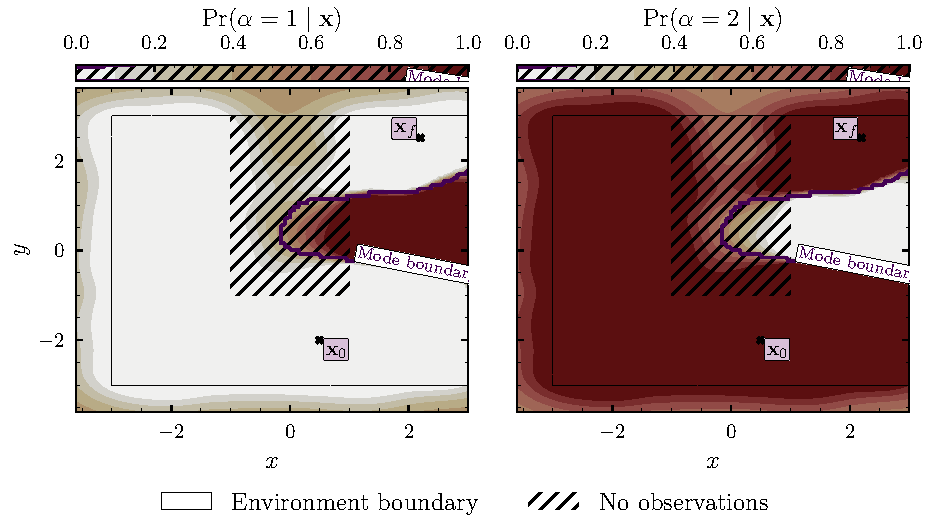
\includegraphics[width=0.98\textwidth]{./images/mode-opt/env/scenario_7/mosvgpe/mixing_probs_no_obs.pdf}
\caption[\acrshort{mosvgpe}'s mixing probabilities after training on simulated quadcopter data set from Environment 1]{
Visualisation of the probability mass function over the expert indicator variable after training \acrshort{mosvgpe}
on the state transition data set from the simulated version of the 2D quadcopter environment
in the illustrative example from \cref{illustrative_example}.
The start state $\state_0$ and target state $\targetState$ are overlayed along with the mode boundary (purple line)
and the subset of the environment which has not been observed (hashed box).}
\label{eq-traj-opt-gating-network-prob-post-inf}
\end{figure}
This section details how the \acrfull{cai_unimodal} framework can be extended to multimodal dynamical systems and
used to encode mode remaining behaviour.
\cref{eq-traj-opt-gating-network-prob-post-inf} shows the probability mass function over the expert indicator variable
after training \acrshort{mosvgpe} on the historical data set of state transitions from the
quadcopter navigation problem in \cref{illustrative_example}.
Intuitively, the goal is to find trajectories that remain in regions of the dynamics with a high probability of
remaining in the desired dynamics mode.

\begin{figure}[t!]
  \centering
   \resizebox{0.4\textwidth}{!}{
   %\resizebox{0.32\textwidth}{!}{
    \begin{tikzpicture}[
      pre/.style={<-,shorten <=0.4pt,>=stealth',semithick},
      post/.style={->,shorten >=0.4pt,>=stealth',semithick}
      ]
      \node[obs] (x1) {$\state_0$};
      \node[latent, right=of x1] (x2) {$\state_1$};
      \node[latent, right=of x2] (x3) {$\state_2$};
      \node[latent, right=of x3] (x4) {$\state_3$};

      \node[latent, above=of x1, xshift=0.6cm] (u1) {$\control_0$};
      \node[latent, right=of u1] (u2) {$\control_1$};
      \node[latent, right=of u2] (u3) {$\control_2$};

      \node[obs, above=of u1] (o1) {$\optimalVar_0$};
      \node[obs, right=of o1] (o2) {$\optimalVar_1$};
      \node[obs, right=of o2] (o3) {$\optimalVar_2$};

      \node[obs, below=of x1] (a1) {$\modeVar_0$};
      \node[obs, right=of a1] (a2) {$\modeVar_1$};
      \node[obs, right=of a2] (a3) {$\modeVar_2$};
      \node[obs, right=of a3] (a4) {$\modeVar_3$};

      \draw[post] (x1)--(x2);
      \draw[post] (x2)--(x3);
      \draw[post] (x3)--(x4);

      \draw[post] (x1)--(u1);
      \draw[post] (x2)--(u2);
      \draw[post] (x3)--(u3);

      \draw[post] (u1)--(x2);
      \draw[post] (u2)--(x3);
      \draw[post] (u3)--(x4);

      \draw[post] (u1)--(o1);
      \draw[post] (x1) to [out=100,in=240] (o1);
      \draw[post] (u2)--(o2);
      \draw[post] (x2) to [out=100,in=240] (o2);
      \draw[post] (u3)--(o3);
      \draw[post] (x3) to [out=100,in=240] (o3);

      \draw[post] (x1)--(a1);
      %\draw[->] (u1) to [out=-90,in=30] (a1);
      \draw[post] (x2)--(a2);
      %\draw[->] (u2) to [out=-90,in=30] (a2);
      \draw[post] (x3)--(a3);
      %\draw[->] (u3) to [out=-90,in=30] (a3);
      \draw[post] (x4)--(a4);
    \end{tikzpicture}
    }
  \caption[Graphical model of control as inference in multimodal dynamical systems]{Graphical model with optimality and mode indicator variables.}
\label{fig-mode-augmented-control-graphical-model}
\end{figure}
\newline

In order to find trajectories that remain in the desired
dynamics mode, this work further augments
the graphical model in \cref{fig-control-graphical-model} with the mode indicator variable \(\modeVar \in \modeDomain\)
from \cref{eq-multimodal-dynamics-disc}.
The resulting graphical model is shown in Figure \ref{fig-mode-augmented-control-graphical-model},
where the evidence is that \(\optimalVar_{\timeInd}=1\) and \(\modeVar_{\timeInd}=\desiredMode\) for
all \(\timeInd \in \{0,\ldots,\TimeInd\}\).
The joint probability model is then given by,
\begin{align} \label{eq-traj-opt-joint-dist-mode}
\jointDist =
&\bigg[ \prod_{\timeInd=0}^{\TimeInd}
\underbrace{\optimalProb}_{\text{cost}}
\underbrace{\modeProb}_{\text{mode remaining term}} \bigg] \nonumber \\
&\bigg[ \prod_{\timeInd=0}^{\TimeInd-1}
\underbrace{\transitionDistK}_{\text{dynamics}}
\underbrace{\controlDist}_{\text{controller}} \bigg],
\end{align}
where \(\modeVarTraj = \{\modeVar_{\timeInd}=\desiredMode \}_{\timeInd=0}^{\TimeInd}\)
denotes every time step of a trajectory belonging to the desired dynamics mode \(\desiredMode\).
\cref{eq-traj-opt-joint-dist-mode} says
that the probability of observing a trajectory is given by taking the product of its probability of occurring
according to the dynamics, with the exponential of the negative cost and the probability of remaining
in the desired dynamics mode.
Given deterministic dynamics, the trajectory with the highest probability will be that with the lowest
cost and highest probability of remaining in the desired dynamics mode.


This work draws on the connection between KL-divergence control \citep{rawlikStochastic2013}
and structured variational inference.
Whilst the derivation shown here differs from \cite{rawlikStochastic2013}, the underlying framework and
objective are the same.

In variational inference, the goal is to approximate a distribution \(p(\mathbf{y})\)
with another, simpler distribution \(q(\mathbf{y})\).
Typically this distribution \(q(\mathbf{y})\) is selected to be a product of conditional distributions connected in a
chain or tree, which lends itself to tractable inference.
In this work, the goal is to approximate the intractable distribution over optimal trajectories,
\begin{align} \label{eq-}
p(\stateTraj, \controlTraj \mid \state_0, \optimalVarTraj, \modeVarTraj)
= Z^{-1}
\Bigg[ \prod_{\timeInd=0}^{\TimeInd}
&\underbrace{\exp \left( - \gamma  \costFunc(\state_\timeInd, \control_\timeInd) \right)}_{\text{cost}}
\underbrace{\modeProb}_{\text{mode remaining term}}
\Bigg]
\nonumber \\
\Bigg[ \prod_{\timeInd=0}^{\TimeInd-1}
&\underbrace{ \transitionDistK}_{\text{dynamics}}
\underbrace{ \policy(\control_\timeInd \mid \state_\timeInd) }_{\text{controller}}
\Bigg]
\end{align}
with the variational distribution \(\trajectoryVarDist\).
Note that \(Z=p(\optimalVarTraj, \modeVarTraj \mid \state_0)\).
In this work the variational distribution over the controller is assumed independent of the state.
That is, instead of parameterising the controller with state feedback, it is parameterised as a set
of open-loop controls \(\controlTraj = \{\control_0, \ldots, \control_{\TimeInd-1}\}\) that are treated as random
variables with density q(\controlTraj).
Calculating \(\trajectoryVarDist\) for a set of controls
\(q(\controlTraj) = \prod_{\timeInd=0}^{\TimeInd-1} \controlVarDist\),
requires simulating the trajectory in the learned,
single-step dynamics model, i.e. making long-term predictions.

\subsubsection{Approximate Inference for Dynamics Predictions}
\label{sec:orgbef7061}

As this method is using a learned representation of the transition dynamics,
it suffices to assume that the dynamics are given by the desired mode's learned dynamics.
Constructing approximate closed-form solutions based on the model in \cref{chap-dynamics}
is difficult, due to the exponential growth in the number of Gaussian components.
Similar to the approach in \cref{sec-dynamics-predictions}, this method obtains multi-step
predictions by cascading single-step predictions through the desired mode's dynamics \acrshort{gp}.
However, this approach extends the predictions to handle normally distributed controls
\(\control_{\timeInd} \sim \mathcal{N}(\controlMean, \controlCov)\).
Multi-step predictions are then obtained by recursively calculating the following integral,
\begin{align} \label{eq-state-control-unc-prop-inf}
\underbrace{q(\state_{\timeInd+1} \mid \state_0, \modeVarTraj_{0:\timeInd})}_{\text{next multi-step state dist}}
%q(\state_{\timeInd+1}) = q(\state_{\timeInd+1} \mid \state_0, \modeVarTraj_{0:\timeInd})
&= \int_{\controlDomain} \int_{\stateDomain}
\underbrace{\transitionDistK}_{\text{single-step dynamics}}
\underbrace{q(\state_\timeInd \mid \state_{0}, \modeVarTraj_{0:\timeInd-1})}_{\text{multi-step state dist}}
\underbrace{q(\control_{\timeInd})}_{\text{control}}
\text{d}\state_{\timeInd}
\text{d}\control_{\timeInd},
\end{align}
using the moment matching approximation from \citep{kussGaussian2006}.
Note that \(\modeVarTraj_{0:\timeInd}\) denotes the first \(\timeInd\) elements of \(\modeVarTraj\), i.e.
\(\modeVarTraj_{0:\timeInd} = \{ \modeVar_i=\desiredMode\}_{i=0}^{\timeInd}\).
Given this method for making multi-step predictions, the variational distribution over state-control trajectories is
given by,
\begin{align} \label{eq-}
%q(\stateTraj, \controlTraj \mid \state_0, \modeVarTraj)
\trajectoryVarDist
= \prod_{\timeInd=0}^{\TimeInd-1}
q(\state_{\timeInd+1} \mid \state_0, \modeVarTraj_{0:\timeInd})
%q(\state_{\timeInd})
\controlVarDist,
\end{align}
with \(q(\state_0) = \delta(\state_0)\).
Note that the state and control at each time step are normally distributed.

\subsubsection{Variational Inference for Sequential Latent Variables}
\label{sec:org68515d7}
Variational inference seeks to optimise \(q(\controlTraj)\)
w.r.t. the \acrfull{elbo}.
In this setup, the evidence is that \(\optimalVar_{\timeInd}=1\) and \(\modeVar_{\timeInd}=\desiredMode\) for
all \(\timeInd \in \{0,\ldots,\TimeInd\}\).
Given this, the \acrshort{elbo} is given by,
\begin{align} \label{eq-}
\text{log} \marginalLikelihood
&= \text{log} \E_{\trajectoryVarDist} \left[ \frac{\jointDist}{\trajectoryVarDist} \right] \nonumber \\
&= \text{log} \E_{\trajectoryVarDist} \left[
\frac{\prod_{\timeInd=0}^{\TimeInd} \left[\optimalProb \modeProb \right]
\prod_{\timeInd=0}^{\TimeInd-1}\controlDist}{\prod_{\timeInd=0}^{\TimeInd-1}  \controlVarDist}
\right] \nonumber \\
&\geq - \sum_{\timeInd=0}^{\TimeInd}
\underbrace{\E_{q(\state_{\timeInd}\mid \state_0, \modeVarTraj_{0:\timeInd-1}) q(\control_{\timeInd} )}
\left[ \costFunc(\state_\timeInd, \control_\timeInd) \right]}_{\text{expected cost}}
+ \sum_{\timeInd=0}^{\TimeInd}
\underbrace{\E_{ q(\state_{\timeInd} \mid \state_0, \modeVarTraj_{0:\timeInd-1})}
\left[ \log \modeProb\right]}_{\text{mode remaining term}} \nonumber \\
&\quad - \sum_{\timeInd=0}^{\TimeInd-1}
\text{KL}\left(\controlVarDist \mid\mid \policy(\control_\timeInd \mid \state_\timeInd) \right)  \coloneqq \mathcal{L}_{\text{mode}},
\end{align}
where the inequality is obtained via Jensen's inequality.
Note the cancellation in the second line where
we assume \(\transitionDistK=q(\state_{\timeInd+1} \mid \state_0, \modeVarTraj_{0:\timeInd})\).
Assuming a uniform prior policy \(\policy(\control_\timeInd \mid \state_\timeInd)\) leads to the \(\text{KL}\)
term reducing to an entropy term and a constant,
\begin{align} \label{eq-traj-opt-elbo}
\mathcal{L}_{\text{mode}} = &-\sum_{\timeInd=0}^{\TimeInd}
\underbrace{\E_{q(\state_{\timeInd} \mid \state_0, \modeVarTraj_{0:\timeInd-1}) \controlVarDist }
\left[ \costFunc(\state_\timeInd, \control_\timeInd) \right]}_{\text{expected cost}}
+ \sum_{\timeInd=0}^{\TimeInd} \underbrace{\E_{ q(\state_{\timeInd} \mid \state_0, \modeVarTraj_{0:\timeInd-1})}
\left[
\log \modeProb \right]}_{\text{mode remaining term}} \nonumber \\
&+ \sum_{\timeInd=0}^{\TimeInd-1} \cancel{\underbrace{\E_{q(\state_{\timeInd} \mid \state_0, \modeVarTraj_{0:\timeInd-1}) \controlVarDist }
\left[\log\policy(\control_{\timeInd} \mid \state_\timeInd)\right]}_{\text{constant}}}
+ \sum_{\timeInd=0}^{\TimeInd-1} \underbrace{H[\control_{\timeInd}]}_{\text{entropy}}.
\end{align}
The \acrshort{elbo} in \cref{eq-traj-opt-elbo} resembles the KL control objective in \cref{eq-kl-control-uniform}
but with an extra term encoding the mode remaining behaviour.
In practice, maximum entropy control is achieved by parameterising the control at each time step to
be normally distributed \({\controlVarDist = \mathcal{N}(\control_{\timeInd} \mid \controlMean, \controlCov)}\).
The control dimensions are assumed independent so \(\controlCov\) becomes diagonal.
The maximum entropy behaviour can be omitted by using deterministic controls, i.e.
parameterising them to follow a Dirac delta distribution \(\controlVarDist = \delta(\control_\timeInd)\).
The control problem is then given by,
\begin{subequations} \label{eq-traj-opt-inference}
\begin{align}
\max_{\controlTraj} &-\sum_{\timeInd=0}^{\TimeInd}
\underbrace{\E_{q(\state_{\timeInd} \mid \state_0, \modeVarTraj_{0:\timeInd-1}) \controlVarDist} \left[ \costFunc(\state_\timeInd, \control_\timeInd) \right]}_{\text{expected cost}}
&+ \sum_{\timeInd=0}^{\TimeInd} \underbrace{\E_{q(\state_{\timeInd} \mid \state_0, \modeVarTraj_{0:\timeInd-1})} \left[
\log \modeProb \right]}_{\text{mode remaining term}} \nonumber \\
 &+ \sum_{\timeInd=0}^{\TimeInd-1} \underbrace{H[\control_{\timeInd}]}_{\text{entropy}} \\
&\text{s.t. \cref{eq-state-control-unc-prop-inf}}
%\text{s.t.}& \quad \cref{eq-state-control-unc-prop-inf}, &
\end{align}
\end{subequations}
which encodes mode remaining behaviour alongside maximum entropy control.
The variational parameters \(\controlMean\) (and \(\controlCov\))
are found by maximising the \acrshort{elbo} using gradient-based optimisation.
At each iteration, the \acrshort{elbo} is calculated by rolling out the control distribution in the
desired mode's \acrshort{gp} dynamics model using \cref{eq-state-control-unc-prop-inf}.
The resulting state-control trajectory is then used to calculate the \acrshort{elbo}.
The cost function is given by,
\begin{align} \label{eq-quadratic-cost-control}
\costFunc(\stateTraj, \controlTraj) &=
\underbrace{(\terminalState - \targetState)^T \terminalStateCostMatrix (\terminalState - \targetState)}_{\text{terminal cost}}
+ \sum_{\timeInd=0}^{\TimeInd-1}
\underbrace{\control_{\timeInd}^T \controlCostMatrix \control_{\timeInd}}_{\text{control cost}},
%\nonumber \\
%&= \| \terminalState - \targetState \|_\terminalStateCostMatrix + \sum_{\timeInd=0}^{\TimeInd-1}
%\| \control_\timeInd \|_\controlCostMatrix
\end{align}
where \(\terminalStateCostMatrix\) and \(\controlCostMatrix\) are user-defined,
real, symmetric, positive semi-definite and positive definite matrices respectively.
This cost function encodes the terminal state boundary condition in \cref{eq-mode-soc-problem} via a
quadratic cost that minimises the deviation of the final state \(\state_{\TimeInd}\) from the target
state \(\targetState\).
Importantly, the expected value of this cost under normally distributed states and controls can be
calculated in closed-form with,
\begin{align} \label{eq-expected-quadratic-cost}
\E_{\stateTraj, \controlTraj} \left[ \costFunc(\stateTraj, \controlTraj) \right] =
(\terminalStateMean - \targetState)^T \terminalStateCostMatrix (\terminalStateMean - \targetState)
+ \text{tr}(\terminalStateCostMatrix \terminalStateCov)
+ \sum_{\timeInd=1}^{\TimeInd-1}
\controlMean^T \controlCostMatrix \controlMean.
+ \sum_{\timeInd=1}^{\TimeInd-1}
\text{tr}(\controlCostMatrix \controlCov )
\end{align}

\section{Conclusion}
\label{sec:org4a73ec7}
This chapter has presented three \emph{mode remaining} trajectory optimisation algorithms.
The first two have shown how the geometry of the \acrshort{mosvgpe} gating network
infers valuable information regarding how a multimodal dynamical system switches between its underlying dynamics modes.
Moreover, they have shown how this latent geometry can be leveraged to encode \emph{mode remaining} behaviour into
two different control strategies.
Both of these control strategies introduce a user tunable parameter \(\lambda\) that can be
tuned to either prioritise remaining in the desired dynamics mode or avoiding regions of high
\emph{epistemic uncertainty}.
However, \cref{chap-traj-opt-results} will show that setting the \(\lambda\) parameter is not straightforward in practice.
The third method presented in this chapter has shown how the probability mass function over the \acrshort{mogpe}'s
expert indicator variable can be used to encode mode remaining behaviour for trajectory optimisation.
In particular, it has shown how the \acrshort{cai} framework \citep{toussaintRobot2009,toussaintProbabilistic2006,kappenOptimal2013}
can be extended to multimodal dynamical systems and how
mode remaining behaviour can be encoded by conditioning on the mode indicator variable.

In \cref{chap-traj-opt-results} the methods presented in this chapter are evaluated and compared using the
quadcopter navigation problem from the illustrative example in \cref{illustrative_example}.
It turns out that in practice, the \acrfull{dre} method from  \cref{sec-traj-opt-energy}
and the \acrfull{cai} method from \cref{chap-traj-opt-inference},
perform significantly better than the \acrfull{ig} method.

\chapter{Quadcopter Experiments - Mode Remaining Trajectory Optimisation \label{chap-traj-opt-results}}
\label{sec:orged9586a}
%\newcommand{\ig}{IG\xspace}
%\newcommand{\dre}{DRE\xspace}
%\newcommand{\cai}{CaI\xspace}
\newcommand{\ig}{DELETEDELETE\xspace}
\newcommand{\dre}{DELETEDELETE\xspace}
\newcommand{\cai}{DELETEDELETE\xspace}
\newcommand{\deltaTime}{\ensuremath{\Delta \timeInd}}
\newcommand{\env}[1]{\ensuremath{\hat{#1}}}
\newcommand{\modeProbTraj}{\ensuremath{\Pr(\allModeVarK \mid \stateTraj)}}

\newcommand{\windDrift}[1]{\ensuremath{\bm\omega_{#1}}}
\newcommand{\windTurbulence}[1]{\ensuremath{\bm\epsilon_{#1}}}
\newcommand{\windTurbulenceNoise}[1]{\ensuremath{\bm\Sigma_{\windTurbulence{#1}}}}
This chapter evaluates the three \emph{mode remaining} trajectory optimisation algorithms:
\begin{enumerate}
\item \acrfull{ig} from \cref{sec-traj-opt-collocation},
\item \acrfull{dre} from \cref{sec-traj-opt-energy},
\item \acrfull{cai} from \cref{sec-traj-opt-inference},
\end{enumerate}
in a simulated version of the illustrative example from \cref{illustrative_example}.
That is, flying a velocity controlled quadcopter from an initial state \(\state_0\), to a target
state \(\state_{f}\), whilst avoiding the turbulent dynamics mode.
The methods are further evaluated on a second simulated velocity controlled quadcopter navigation problem.
See \cref{fig-environments} for schematics of the two environments.
The turbulent dynamics modes (green) are subject to higher drift due to the wind field created by the fan.
They are also subject to higher diffusion (process noise) resulting from the turbulence induced by the fan.
Although the exact turbulent dynamics are \emph{unknown}, they are believed to be difficult to control.
This is due to the high process noise which may lead to catastrophic failure.
Therefore, it is desirable to find trajectories that avoid entering this turbulent dynamics mode.

\begin{figure}[h!]
    \centering
    \begin{minipage}[r]{0.49\columnwidth}
        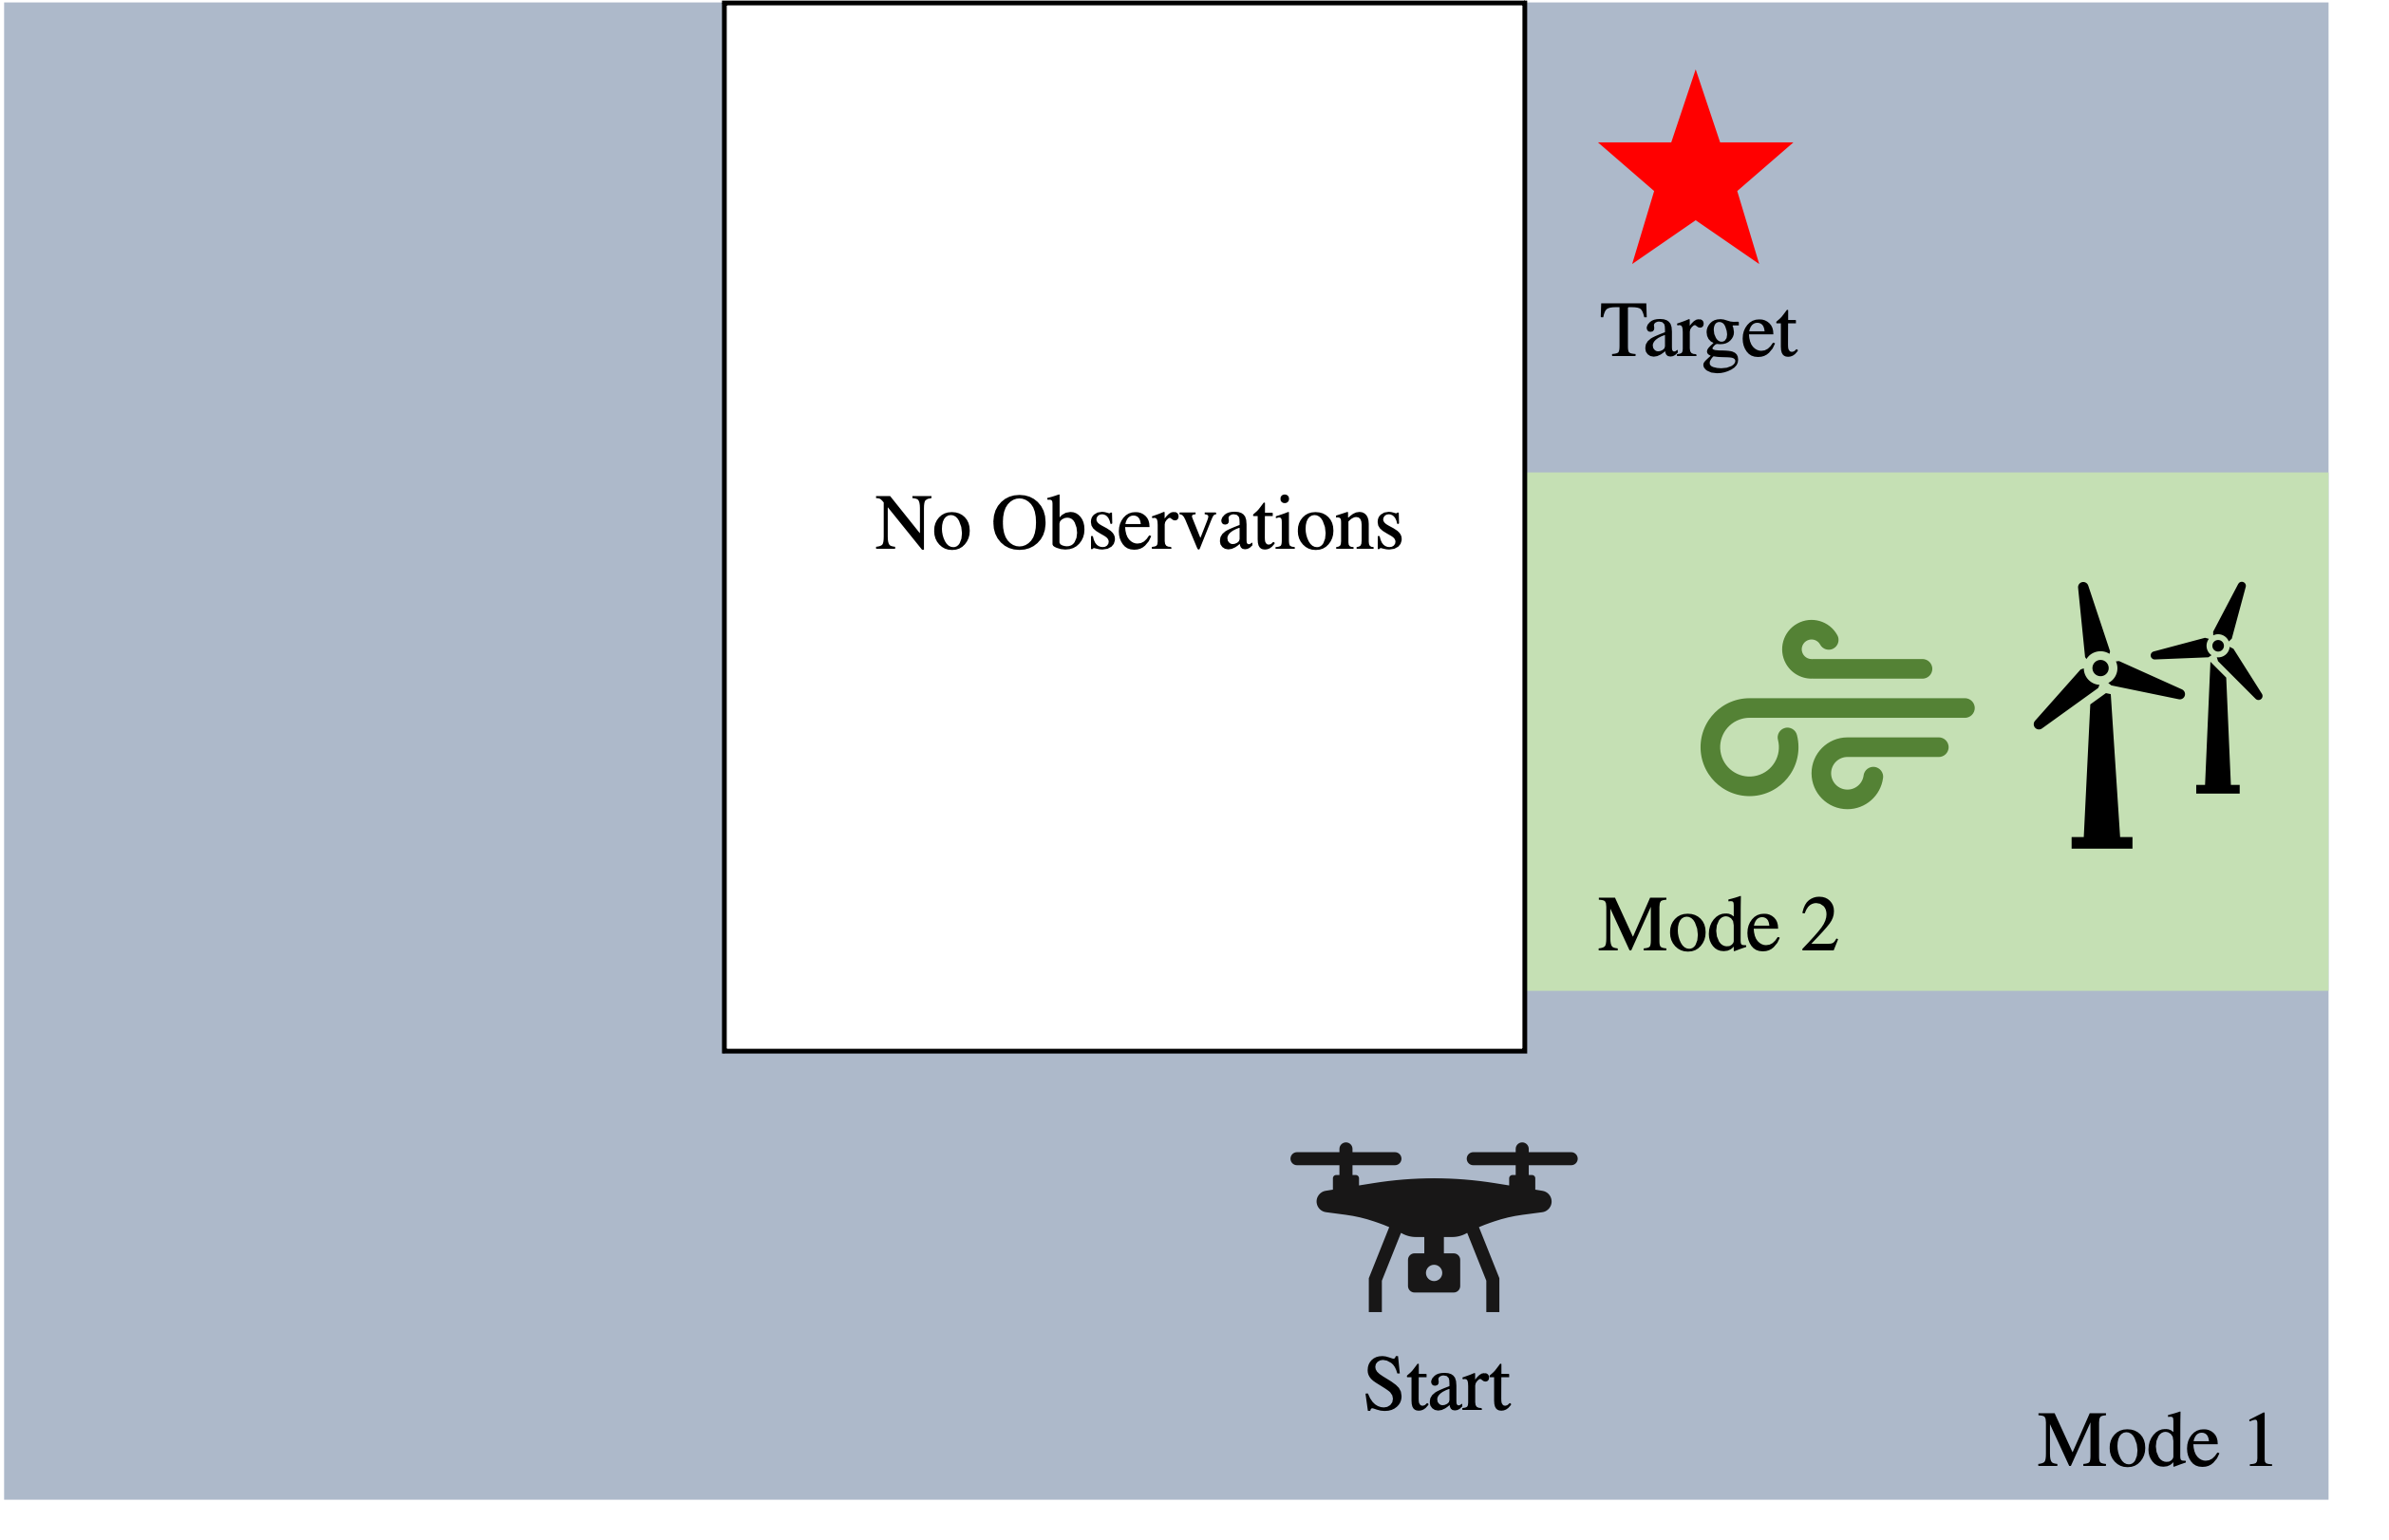
\includegraphics[width=\textwidth]{./images/quadcopter-domain-collocation-ppt.png}
        \subcaption{Environment 1}
        \label{fig-environment-1}
    \end{minipage}
    \begin{minipage}[r]{0.49\columnwidth}
        %\includegraphics[width=\textwidth]{./images/point-mass-problem-statement-scenario-4.pdf}
        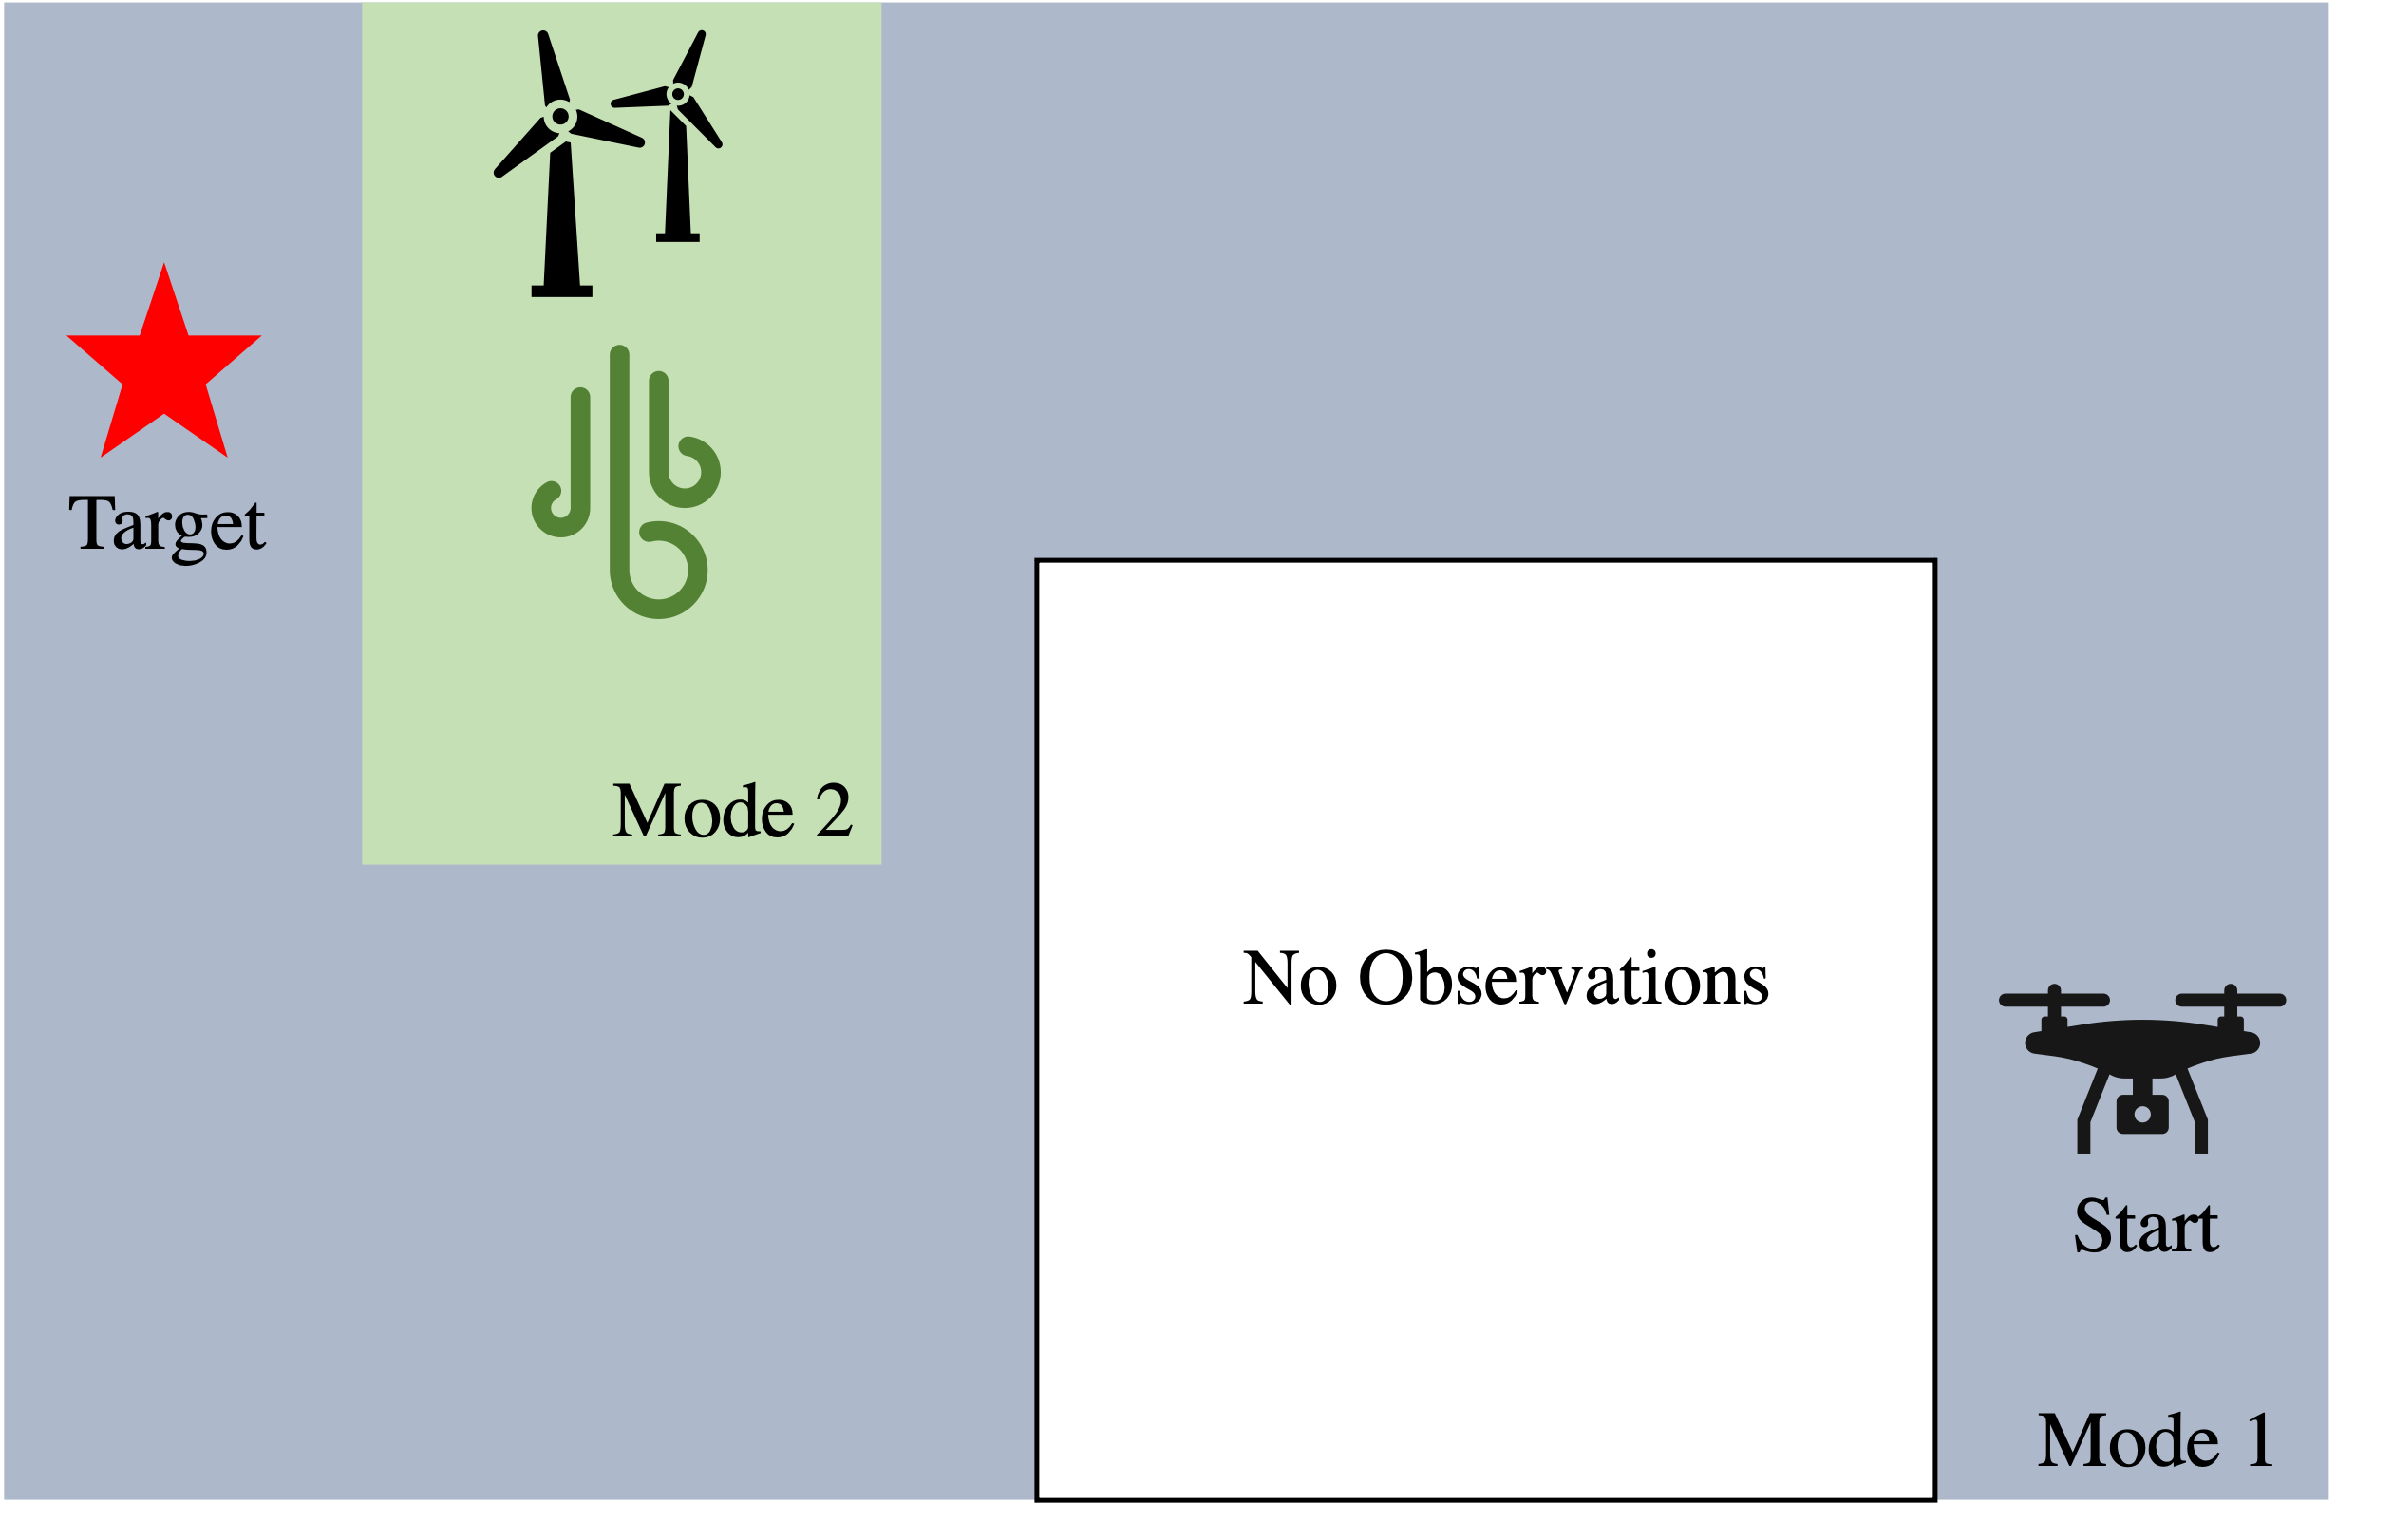
\includegraphics[width=\textwidth]{./images/quadcopter-domain-environment-2.png}
        \subcaption{Environment 2}
        \label{fig-environment-2}
    \end{minipage}
    \caption[Diagrams illustrating two quadcopter navigation problems]{Visualisation of two quadcopter navigation problems in environments with different spatially
    varying modes.
    It shows the desired dynamics mode in blue (Mode 1) and
    the turbulent dynamics mode induced by a fan in green (Mode 2).
    The white box indicates a region of the environment which was not observed.
    The goal is to navigate from the start state $\state_0$, to the target state $\targetState$, whilst remaining
    in the desired dynamics mode (Mode 1).}
    \label{fig-environments}
\end{figure}

The collocation solver from the \acrfull{ig} method in \cref{chap-traj-opt-geometry}
is tested on a real-world quadcopter state transition data set.
This data set was collected with constant controls so the controls could not be recovered from
the full \acrshort{mosvgpe} dynamics model, nor could the \acrfull{dre}
method from \cref{chap-traj-opt-geometry} or the \acrfull{cai} method from
\cref{chap-traj-opt-inference} be tested.
Nevertheless, the results are a small step towards validating the method's applicability to real-world systems.
All three control methods are tested in the two simulated environments so that they can be compared.
To aid comparison with the real-world experiments, the layout of the first simulated environment  (Environment 1)
was kept consistent with the real-world experiments.
\section{Real-World Quadcopter Experiments \label{sec-traj-opt-results-brl}}
\label{sec:org89b1fab}
The \acrfull{ig} method presented in \cref{sec-traj-opt-collocation} was evaluated
using data from the real-world quadcopter navigation problem detailed in \cref{sec-brl-experiment}.
However, a different subset of the environment was not observed
and the model was trained using an old variational inference scheme, not the one presented in \cref{chap-dynamics}.
\cref{fig-environment-1} shows the environment and details the quadcopter navigation problem.
The controls were kept constant during data collection, reducing the dynamics to
\(\Delta \state_{\timeInd+1} = \dynamicsFunc(\state_{\timeInd}; \control_{\timeInd}=\fixedControl)\).
See \cref{sec-brl-experiment} for more details on data collection and processing.

\begin{figure}[!t]
\centering
\begin{minipage}[r]{\columnwidth}
\centering
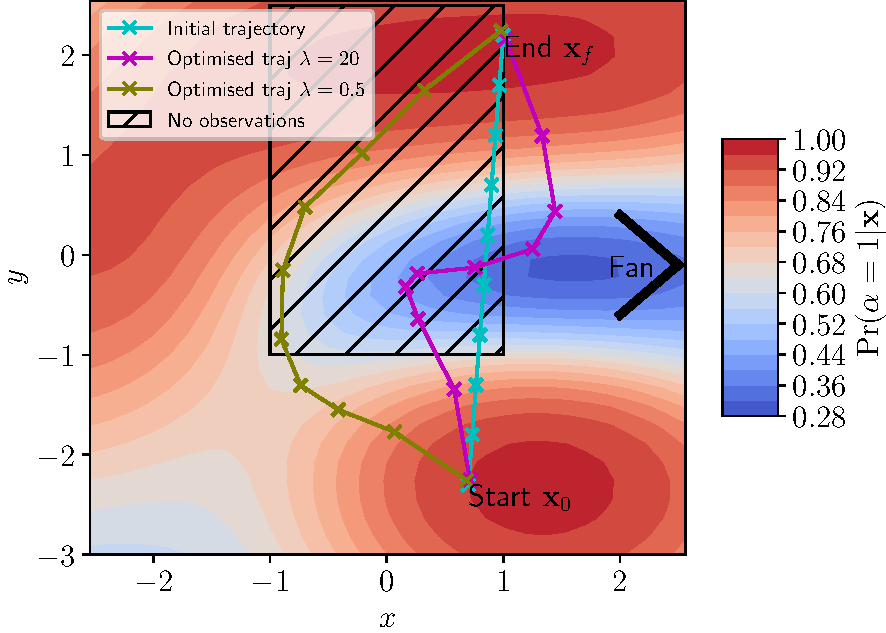
\includegraphics[width=0.7\textwidth]{./images/geometric-traj-opt-over-prob.pdf}
\subcaption{Desired mode's mixing probability.}
\label{fig-geometric-traj-opt-over-prob}
\end{minipage}
\begin{minipage}[r]{\columnwidth}
\centering
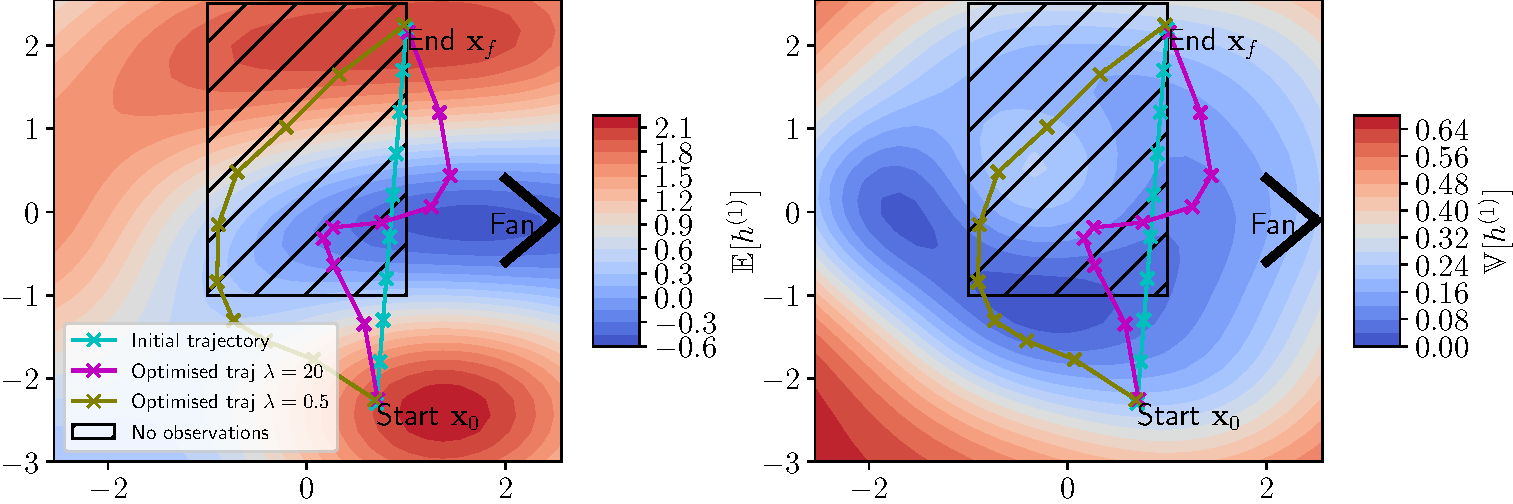
\includegraphics[width=\textwidth]{./images/geometric-traj-opt-over-svgp.pdf}
\subcaption{\acrshort{gp} posterior mean (left) and variance (right) over the desired mode's gating function.}
\label{fig-geometric-traj-opt-over-svgp}
\end{minipage}
\caption[\acrfull{ig} trajectory optimisation results in real-world quadcopter experiments over gating network posterior]{\textbf{\acrfull{ig}} trajectory optimisation results after solving the nonlinear
program in \cref{eq-collocation-problem}
using the desired mode's ($\modeVar=1$) gating function from the \acrshort{mosvgpe} (with $\ModeInd=2$ experts)
after training on the real-world velocity controlled quadcopter data set.
The initial (cyan) and optimised trajectories' -- for two settings of $\lambda$ -- are
overlayed on the desired mode's (\subref{fig-geometric-traj-opt-over-prob}) mixing probability and
(\subref{fig-geometric-traj-opt-over-svgp}) gating function \acrshort{gp} posterior.}
\label{fig-geometric-traj-opt}
\end{figure}

\subsection{Model Learning}
\label{sec:org26445c3}
The model from \cref{chap-dynamics} was instantiated with \(\ModeInd=2\) experts and trained on
the data collected from the velocity controlled quadcopter experiment.
Each mode's dynamics \acrshort{gp} used a Squared Exponential kernel with \acrfull{ard} and a constant mean function.
The gating network used a single gating function with a Bernoulli likelihood.
Its \acrshort{gp} prior utilised a Squared Exponential kernel with \acrshort{ard} and a zero mean function.

\cref{fig-geometric-traj-opt} shows the gating network posterior where the model has learned
two dynamics modes, characterised by the drift and process noise induced by the fan.
Mode 1 (red) represents the operable dynamics mode whilst Mode 2 (blue)
represents the inoperable turbulent dynamics mode.
This is illustrated in \cref{fig-geometric-traj-opt-over-prob} which shows the probability that
the desired mode (\(\modeVar = 1\)) governs the dynamics over the domain.
\cref{fig-geometric-traj-opt-over-svgp} shows the \acrshort{gp} posterior mean (left) and variance (right) of the
gating function \(\gatingFunc_1\) associated with the desired dynamics mode.
The mean is high where the model believes the desired mode is responsible for predicting, low where it
believes another mode is responsible and zero where it is uncertain.
The variance (right) has also clearly captured information regarding the \emph{epistemic uncertainty},
i.e. where the model is uncertain which mode governs the dynamics.

\subsection{Trajectory Optimisation using Indirect Optimal Control via Latent Geodesics}
\label{sec:org993dc37}
The initial (cyan) trajectory in \cref{fig-geometric-traj-opt} was initialised as a straight line with
\(10\) collocation points, indicated by the crosses.
The collocation solver guarantees that trajectories end at the target state.
However, trajectories are not guaranteed to remain in the desired dynamics mode, nor are they guaranteed to
satisfy the system dynamics.
\cref{tab-results} compares the initial trajectory to the results obtained
with two settings of the \(\lambda\) parameter from \cref{eq-expected-metric-weighting},
which determines the relevance of the covariance term in the expected Riemannian metric.
\begin{table}[!t]
\caption[Comparison of \acrfull{ig} experiments on real-world quadcopter]{\label{tab-results}\textbf{\acrfull{ig}} Comparison of performance with different settings of \(\lambda\). The performance measures are summed over collocation points.}
\centering
\begin{tabular}{lll}
\hline
Trajectory & Mixing Probability & Epistemic Uncertainty\\
 & \(\sum_{i=1}^{I} \Pr(\modeVar_i=1 \mid \state_i)\) & \(\sum_{i=1}^{I} \mathbb{V}[\gatingFunc_{1}(\state_i)]\)\\
\hline
Initial & \(7.480\) & \(1.345\)\\
Optimised \(\lambda=20.0\) & \(6.091\) & \(\mathbf{1.274}\)\\
Optimised \(\lambda=0.5\) & \(\mathbf{8.118}\) & \(1.437\)\\
\end{tabular}
\end{table}

\begin{figure}[b!]
\centering
\begin{minipage}[r]{0.49\columnwidth}
\centering
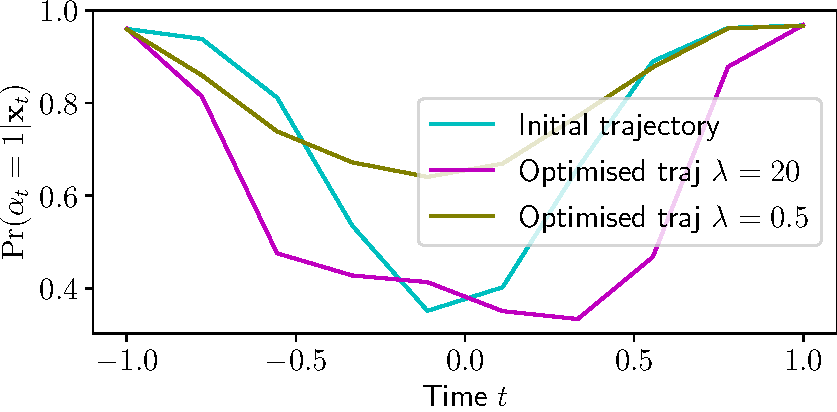
\includegraphics[width=\textwidth]{./images/geometric-traj-opt-prob-vs-time.pdf}
\subcaption{Desired mode's (\modeVar=1) mixing probability over the trajectories.}
\label{fig-mixing_prob_vs_time}
\end{minipage}
\begin{minipage}[r]{0.49\columnwidth}
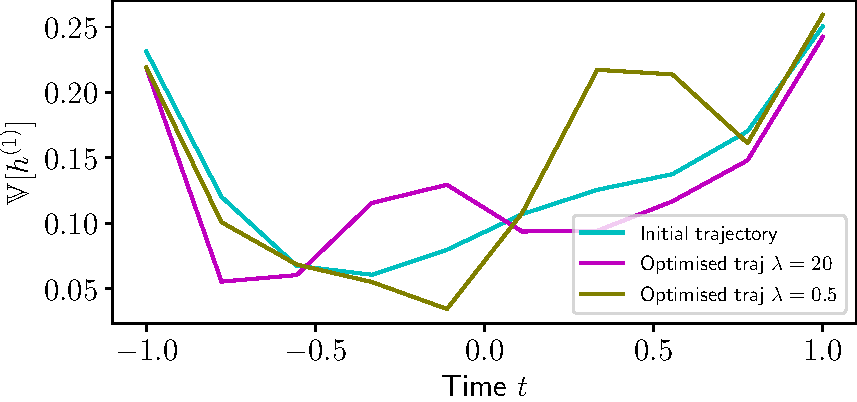
\includegraphics[width=\textwidth]{./images/geometric-traj-opt-epistemic-vs-time.pdf}
%\label{}
\subcaption{Posterior variance associated with the desired mode's (\modeVar=1) gating function over the trajectories.}
\label{fig-epistemic_var_vs_time}
\end{minipage}
\caption[\acrfull{ig} trajectory optimisation results in real-world quadcopter experiments - performance vs time]{\textbf{\acrfull{ig}} Comparision of the initial and optimised trajectories' performance -- for two
settings of $\lambda$ -- at a) staying in the desired mode and b) avoiding regions of the gating network
with high epistemic uncertainty.}
\label{fig-metric-vs-time}
\end{figure}
\newline

The higher probability of remaining in the desired dynamics mode indicates that
the lower setting of \(\lambda=0.5\) exhibits more mode remaining behaviour.
This can be seen visually in \cref{fig-geometric-traj-opt-over-prob}, where the trajectory with \(\lambda=0.5\)
remains in regions of the model with high probability.
The right-hand plot in \cref{fig-geometric-traj-opt-over-svgp}
shows that this trajectory favours remaining in the desired mode at the cost of entering the region
of the gating network with high \emph{epistemic uncertainty}.
This is quantified in \cref{tab-results}, which shows it accumulates more gating function variance than both the
initial trajectory and the trajectory found with \(\lambda=20.0\).

In contrast, the trajectory found with \(\lambda=20.0\) initially remains in the desired mode
but then enters the turbulent mode in favour of avoiding the area of high \emph{epistemic uncertainty}.
This is confirmed in \cref{tab-results} as the trajectory found with \(\lambda=20.0\) accumulates the least gating
function variance over the trajectory.
This is further visualised in \cref{fig-epistemic_var_vs_time,fig-mixing_prob_vs_time}.
These results align with the intended behaviour of the user tunable \(\lambda\) parameter.
However, in this experiment, increasing the relevance of the covariance term in the expected Riemannian
metric has no benefit.
This is because it pushes the trajectory into the turbulent dynamics mode.

These results indicate the nonlinear program in \cref{eq-collocation-problem},
i.e. solving the geodesic \acrshort{ode} in \cref{eq-2ode} via collocation, is capable of finding state
trajectories from \(\state_0\) to \(\targetState\) that exhibit mode remaining behaviour.
However, these experiments have not validated the method's ability to recover the controls from the state trajectory
using \cref{eq-control-elbo}.
This is because a full transition dynamics model has not been learned so the control trajectory cannot be recovered.
In \cref{sec-traj-opt-results-simulated} the method is evaluated in a simulated environment
where its ability to recover the controls is tested.

It is worth noting here that the mode remaining behaviour is
sensitive to the tolerance on the collocation constraints.
Setting the tolerance too small often resulted in the solver failing to converge, whilst setting the tolerance too
large omitted any mode remaining behaviour.

\section{Simulated Quadcopter Experiments \label{sec-traj-opt-results-simulated}}
\label{sec:org1d8a901}
All of the control methods are now tested in two simulated environments so that they can be compared.
This section first details the two simulation environments.

\subsection{Simulator Setup}
\label{sec:org77a8100}
The simulated environments have two dynamics modes, \(\modeVar \in \{1, 2\}\), whose
transition dynamics are given by a single integrator discretised using the forward Euler method
(velocity times time).
The modes are induced by different wind fields which are characterised by their
drift \(\windDrift{\modeInd}\) and process noise \(\windTurbulence{\modeInd}\) terms.
Each mode's dynamics are given by,
\begin{align}
\mode{\dynamicsFunc}(\state_\timeInd, \control_\timeInd; \Delta\timeInd=0.25)
&= \state_{\timeInd} + \control_{\timeInd} \times \Delta\timeInd + \windDrift{\modeInd} + \windTurbulence{\modeInd} \\
%\quad \text{if} \quad \modeVar_\timeInd = \modeInd \\
\windTurbulence{\modeInd} &\sim \mathcal{N}(\bm0, \windTurbulenceNoise{\modeInd}).
\end{align}
The state domain is constrained to \(x, y \in [-3, 3]\) and min/max controls are implemented by constraining the
control domain to \(\velocity_x, \velocity_y \in [-5, 5]\).


\textbf{Data set}
We sampled \(4000\) state transitions from each environment with \(\Delta \timeInd = 0.25s\).
We then removed a subset of the state transitions to induce a region of high \emph{epistemic uncertainty} in the
learned dynamics model.
This enabled the methods' ability to avoid regions of high \emph{epistemic uncertainty} to be tested.
\cref{fig-dataset-scenario-both} shows the two environments as well as the state transition data sets that were
sampled from them.
In Environment 2, the turbulent dynamics mode and the unobserved regions are in different locations to
Environment 1.
Further to this, the region with no observations does not overlap the mode boundary like in Environment 1.

\begin{figure}
\centering
\begin{minipage}[r]{0.47\columnwidth}
\centering
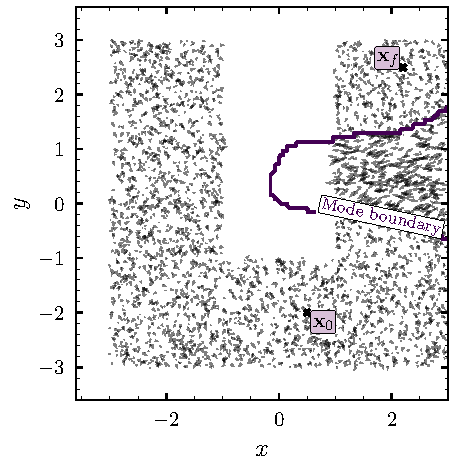
\includegraphics[width=1\textwidth]{./images/mode-opt/env/scenario_7/env_with_dataset_start_end_pos.pdf}
\subcaption{\textbf{Environment 1} -
$\windDrift{1} = \{0.02, -0.4\}$, $\windDrift{2} = \{-2.0, -0.4\}$,
$\windTurbulenceNoise{1} = \diag\left([0.0002, 0.0001]\right)$ and
$\windTurbulenceNoise{2} = \diag\left([0.2, 0.05]\right)$}
\label{fig-dataset-scenario-7}
\end{minipage}
\begin{minipage}[r]{0.47\columnwidth}
\centering
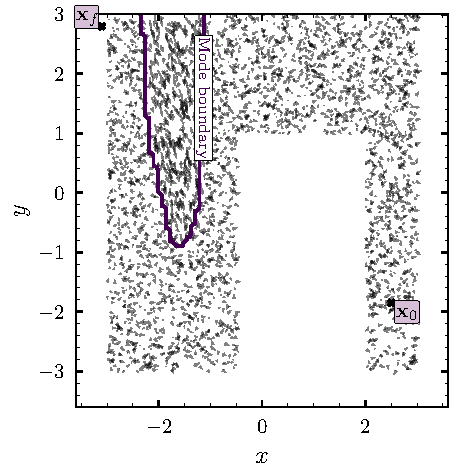
\includegraphics[width=1\textwidth]{./images/mode-opt/env/scenario_5/env_with_dataset_start_end_pos.pdf}
\subcaption{\textbf{Environment 2} -
$\windDrift{1} = \{0.4, 0.02\}$, $\windDrift{2} = \{0.4, -2.0\}$,
$\windTurbulenceNoise{1} = \diag\left([0.0001, 0.0002]\right)$ and
$\windTurbulenceNoise{2} = \diag\left([0.05, 0.2]\right)$}
\label{fig-dataset-scenario-5}
\end{minipage}
\caption[Diagram of two simulated environments]{\textbf{Simulated Environments} - Visualisation of the simulated environments with their true mode boundaries
indicated by the purple lines.
The state transition data set sampled from each environment is visualised by the quiver plots.
The initial $\state_0$ and target states $\targetState$ for the trajectory optimisation are overlayed.}
\label{fig-dataset-scenario-both}
\end{figure}
\subsection{Model Learning}
\label{sec:orgf0670fd}
Following the experiments in \cref{sec-traj-opt-results-brl},
the model from \cref{chap-dynamics} was instantiated with \(\ModeInd=2\) experts, one to
represent the desired dynamics mode and one to represent the turbulent dynamics mode.
The experiments used the same \acrshort{gp} priors and hyperparameters as the real-world experiments
in \cref{sec-traj-opt-results-brl}.
However, in contrast to the real-world experiments, the simulated experiments presented here learn the full transition
dynamics model, i.e. they do not assume constant controls.
\cref{fig-traj-opt-gating-network-7,fig-traj-opt-gating-network-5} show the gating network posteriors after training
on the data sets from Environment 1 and Environment 2 respectively.
In both environments,
Expert 1 represents the turbulent dynamics mode and Expert 2 represents the operable, desired dynamics mode.
This results from Expert 1 learning much higher drift and process noise than Expert 2.

\begin{figure}[h!]
\centering
\begin{minipage}[r]{\columnwidth}
\centering
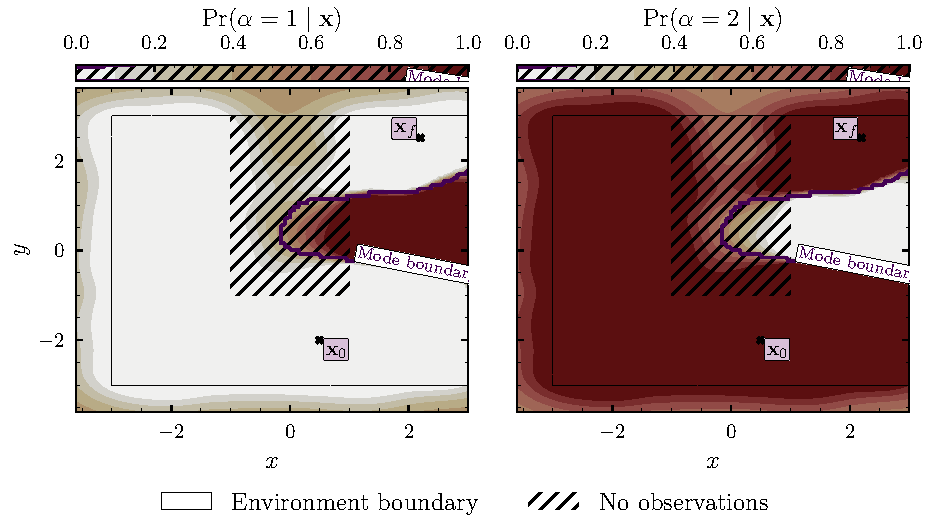
\includegraphics[width=0.98\textwidth]{./images/mode-opt/env/scenario_7/mosvgpe/mixing_probs_no_obs.pdf}
\subcaption{Mixing probabilities}
\label{eq-traj-opt-gating-network-prob-post-7}
\end{minipage}
\begin{minipage}{1.0\textwidth}
\centering
\includegraphics[width=0.98\textwidth]{./images/mode-opt/env/scenario_7/mosvgpe/desired_gating_gp_no_obs.pdf}
\subcaption{Gating function's \acrshort{gp} posterior}
\label{eq-traj-opt-gating-network-gp-post-7}
\end{minipage}
\caption[Environment 1 gating network posterior]{\textbf{Environment 1} Visualisation of the gating network posterior after training \acrshort{mosvgpe}
on the state transition data set from Environment 1.
(\subref{eq-traj-opt-gating-network-prob-post-7}) shows the probability mass function over the expert indicator
variable and (\subref{eq-traj-opt-gating-network-gp-post-7}) shows the gating function's \acrshort{gp}
posterior mean (left) and posterior variance (right).
The start state $\state_0$ and target state $\targetState$ are overlayed along with the mode boundary (purple line)
and the subset of the environment which has not been observed (hashed box).}
\label{fig-traj-opt-gating-network-7}
\end{figure}

\begin{figure}[h!]
\centering
\begin{minipage}[r]{\columnwidth}
\centering
\includegraphics[width=0.98\textwidth]{./images/mode-opt/env/scenario_5/mosvgpe/mixing_probs_no_obs.pdf}
\subcaption{Mixing probabilities}
\label{eq-traj-opt-gating-network-prob-post-5}
\end{minipage}
\begin{minipage}{1.0\textwidth}
\centering
\includegraphics[width=0.98\textwidth]{./images/mode-opt/env/scenario_5/mosvgpe/desired_gating_gp_no_obs.pdf}
\subcaption{Gating function's \acrshort{gp} posterior}
\label{eq-traj-opt-gating-network-gp-post-5}
\end{minipage}
\caption[Environment 2 gating network posterior]{\textbf{Environment 2} Visualisation of the gating network posterior after training \acrshort{mosvgpe}
on the state transition data set from Environment 2.
(\subref{eq-traj-opt-gating-network-prob-post-5}) shows the probability mass function over the expert indicator
variable and (\subref{eq-traj-opt-gating-network-gp-post-5}) shows the gating function's \acrshort{gp}
posterior mean (left) and posterior variance (right).
The start state $\state_0$ and target state $\targetState$ are overlayed along with the mode boundary (purple line)
and the subset of the environment which has not been observed (hashed box).}
\label{fig-traj-opt-gating-network-5}
\end{figure}
\subsection{Performance Indicators}
\label{sec:org84f92ea}
Before evaluating the three trajectory optimisation algorithms in the simulated environments,
let us restate the goals from \cref{chap-traj-opt-control}:
\begin{description}
\item[{Goal 1}] Navigate to the target state \(\targetState\),
\item[{Goal 2}] Remain in the operable, desired dynamics mode \(\desiredMode\),
\item[{Goal 3}] Avoid regions of the learned dynamics with high \emph{epistemic uncertainty},
\begin{description}
\item[{Goal 3.1}] in the desired dynamics mode  \(\latentFunc_{\desiredMode}\), i.e. where the underlying dynamics are not known,
\item[{Goal 3.2}] in the gating network \(\modeVar\), i.e. where it is not known which mode governs the dynamics.
\end{description}
\end{description}

The performance of the trajectory optimisation algorithms are evaluated
using four performance indicators:
\begin{enumerate}
\item Goal 2 is measured using the probability of remaining in the desired mode without the model's uncertainty marginalised,
\begin{align} \label{eq-mode-probability-no-unc}
\sum_{\timeInd=0}^{\TimeInd} \Pr(\modeVar_\timeInd=\desiredMode \mid \gatingFunc(\state_{0:\timeInd}), \state_{0:\timeInd}, \control_{0:\timeInd}, \modeVar_{0:\timeInd-1}=\desiredMode)
\end{align}
This probability will only decrease when a trajectory leaves the desired mode.
\item Goal 3.1 is measured using the state variance accumulated from cascading single-step predictions,
\begin{align} \label{eq-metric-state-var}
\mathbb{V}[\stateTraj] = \sum_{\timeInd=1}^{\TimeInd} \mathbb{V}[\state_{\timeInd}].
\end{align}
This will increase when a trajectory passes through regions of the desired dynamics mode with high \emph{epistemic uncertainty}.
\item Goal 3.2 is measured using the gating function variance accumulated from cascading single-step predictions,
\begin{align} \label{eq-metric-gating-var}
\mathbb{V}[\desiredGatingFunction(\stateTraj)] = \sum_{\timeInd=1}^{\TimeInd}
\mathbb{V}[\desiredGatingFunction(\state_{\timeInd})].
\end{align}
This will increase when a trajectory passes through regions of the gating network with high \emph{epistemic uncertainty}.
\item Probability of remaining in the desired mode with the model's uncertainty marginalised,
calculated using \cref{eq-mode-chance-constraint-integral},
\begin{align} \label{eq-mode-probability-all-unc}
\sum_{\timeInd=1}^{\TimeInd}
\Pr(\modeVar_\timeInd=\desiredMode \mid \state_0, \control_{0:\timeInd}, \modeVar_{0:\timeInd-1}=\desiredMode).
\end{align}
This probability will decrease when a trajectory leaves the desired mode and when it
passes through regions of the learned dynamics with high uncertainty.
\end{enumerate}
The methods' ability to remain in the desired dynamics mode \(\desiredMode\), that is, to accomplish Goal 2,
is measured using the probability of remaining in the desired dynamics mode \cref{eq-mode-probability-no-unc}.
The secondary goal of avoiding regions of the learned dynamics model with high \emph{epistemic uncertainty}
in the desired dynamics mode (Goal 3.1), is measured by summing the state variance
over each trajectory \cref{eq-metric-state-var}.
Similarly, each method's ability to avoid regions of the gating network with high epistemic
uncertainty in the gating network (Goal 3.2),
is measured by summing the gating function variance over each trajectory \cref{eq-metric-gating-var}.
Intuitively, the goal is to maximise the probability of being in the desired mode,
whilst minimising the variance accumulated over a trajectory.
This corresponds to maximising the probability of remaining in the desired dynamics mode
with all of the model's \emph{epistemic uncertainty} marginalised, i.e. maximising \cref{eq-mode-probability-all-unc}.

\begin{table}
\caption[Trajectory optimisation results in simulated environments]{\textbf{Results in simulated environments} Comparison of the \acrfull{ig} method from \cref{sec-traj-opt-collocation}, the \acrfull{dre} method from \cref{sec-traj-opt-energy} and the \acrfull{cai} method from \cref{sec-traj-opt-inference}, with max entropy (\acrshort{cai} gauss) and without max entropy (\acrshort{cai} Dirac). All methods are evaluated in the two simulated environments. The performance measures are summed over the collocation points for the \acrshort{ig} method and over each time step for the \acrshort{dre} method and the \acrshort{cai} method. The "Mode prob" column calculates the probability of being in the desired dynamics mode at each time step without marginalising the state and gating function uncertainty over the trajectory. In contrast the "Mode prob with unc." marginalises both the state and gating function uncertainty at each time step. The target state column indicates if the trajectory reached the target state in the environment ($\checkmark$ both), only under the desired mode's dynamics \acrshort{gp} ($\checkmark$ dynamics) or not at all ($\times$).}
\label{tab-results-sim-envs}
\resizebox{\textwidth}{!}{
\begin{center}
\begin{tabular}{clccccccc}
\hline
Env & Method & \(\lambda\) & Mode prob & Mode prob with unc. & State unc. & Gating unc. & Target state\\
 &  &  & Eq. \ref{eq-mode-probability-no-unc} & Eq. \ref{eq-mode-probability-all-unc} & \(\mathbb{V}[\stateTraj]\) & \(\mathbb{V}[\gatingFunc_{\desiredMode}(\stateTraj)]\) & \(\state_{\TimeInd}==\targetState\)?\\
\hline
 & \acrshort{ig} & \(0.5\) & \(16.96\) & \(16.22\) & \(8.69\) & \(346.62\) & \(\times\) dynamics\\
 & \acrshort{ig} & \(1.0\) & \(18.51\) & \(16.98\) & \(8.70\) & \(367.16\) & \(\times\) dynamics\\
 & \acrshort{ig} & \(20.0\) & \(15.04\) & \(14.92\) & \(8.65\) & \(231.98\) & \(\times\) dynamics\\
1 & \acrshort{dre} & \(0.5\) & \(\mathbf{20.98}\) & \(18.04\) & \(8.71\) & \(388.71\) & \(\checkmark\) both\\
 & \acrshort{dre} & \(1.0\) & \(\mathbf{20.98}\) & \(18.10\) & \(8.72\) & \(370.94\) & \(\checkmark\) both\\
 & \acrshort{dre} & \(20.0\) & \(13.47\) & \(13.10\) & \(\mathbf{8.64}\) & \(\mathbf{164.88}\) & \(\times\) dynamics\\
 & \acrshort{cai} (gauss) & N/A & \(20.94\) & \(\mathbf{19.99}\) & \(8.74\) & \(208.62\) & \(\checkmark\) both\\
 & \acrshort{cai} (Dirac) & N/A & \(20.96\) & \(19.58\) & \(8.73\) & \(258.27\) & \(\checkmark\) both\\
\hline
 & \acrshort{ig} & \(0.5\) & \(18.98\) & \(19.22\) & \(1.53\) & \(495.11\) & \(\times\)\\
 & \acrshort{ig} & \(1.0\) & \(18.98\) & \(19.16\) & \(1.39\) & \(522.60\) & \(\times\)\\
 & \acrshort{ig} (mid point) & \(1.0\) & \(17.55\) & \(17.80\) & \(1.57\) & \(553.00\) & \(\times\)\\
 & \acrshort{ig} & \(5.0\) & \(18.98\) & \(19.17\) & \(1.44\) & \(503.94\) & \(\times\)\\
2 & \acrshort{dre} & \(0.5\) & \(20.96\) & \(20.34\) & \(1.42\) & \(367.47\) & \(\checkmark\) both\\
 & \acrshort{dre} & \(1.0\) & \(\mathbf{20.98}\) & \(20.68\) & \(\mathbf{1.28}\) & \(\mathbf{334.47}\) & \(\checkmark\) both\\
 & \acrshort{dre} & \(5.0\) & \(20.81\) & \(20.13\) & \(1.37\) & \(374.13\) & \(\checkmark\) both\\
 & \acrshort{cai} (gauss) & N/A & \(\mathbf{20.98}\) & \(\mathbf{20.72}\) & \(1.75\) & \(596.67\) & \(\checkmark\) both\\
 & \acrshort{cai} (Dirac) & N/A & \(\mathbf{20.98}\) & \(20.61\) & \(1.56\) & \(644.35\) & \(\checkmark\) both\\
\end{tabular}
\end{center}
}
\end{table}

\subsection{Results}
\label{sec:org77bb2f2}
Three settings of the tunable \(\lambda\) parameter were tested for
both of the geometry-based methods in each environment.
The \acrfull{cai} method from \cref{sec-traj-opt-inference} was tested with
Gaussian controls (gauss) and with deterministic (Dirac) controls.
This enabled the maximum entropy control behaviour (resulting from Gaussian controls)
to be compared to a baseline without maximum entropy control.
\cref{tab-results-sim-envs} summarises all of the results from both environments.

\textbf{Initialisation} All of the \acrfull{dre} and \acrfull{cai} experiments used
a horizon of \(\TimeInd=20\) time steps and
all of the \acrfull{ig} experiments were initialised with \(I=20\) collocation points.
Further to this, all of the \acrshort{ig} experiments were initialised
with straight line trajectories between \(\state_0\) and
\(\targetState\), except for one experiment in Environment 2, named \acrshort{ig} \(\lambda\)=1.0 (mid point), which was initialised
with two straight lines, between \(\state_0\), \([-2.0, -2.0]\) and \(\targetState\).
This is because the \acrshort{ig} experiments struggled to find solutions in Environment 2
-- due to local optima -- without adjusting the initial solution.

\textbf{Visualisation}
\cref{fig-all-traj-opt-prob,fig-all-traj-opt-mean,fig-all-traj-opt-variance}
show the trajectory optimisation results for both environments overlayed on their associated gating network posteriors.
In each figure, the left-hand column shows results for Environment 1
whilst the right-hand column shows the results for Environment 2.
The figures show the state trajectories obtained from cascading single-step predictions through
the desired mode's  \acrshort{gp} dynamics
using the controls found by the \acrshort{ig} method (top row), the
\acrshort{dre} method (middle row) and the \acrshort{cai} method (bottom row).
\cref{fig-all-traj-opt-prob} shows the optimised trajectories overlayed on the desired
mode's (\(\modeVar=2\)) mixing probability.
This is useful for seeing how well trajectories remain in regions of the learned dynamics model with high
probability of being in the desired mode.
\cref{fig-all-traj-opt-mean} shows the trajectories overlayed on the gating function's posterior mean.
As the geometry-based methods in this chapter are based on finding shortest trajectories on this manifold,
the posterior mean plot is useful for observing contour following behaviour.
As the methods should find trajectories that avoid regions of the gating network with
high \emph{epistemic uncertainty}, \cref{fig-all-traj-opt-variance} shows them
overlayed on the gating function's posterior variance.
Because the \acrshort{ig} method is a two-stage process, which first finds a state trajectory using
the collocation solver and then recovers the controls using the inference strategy in \cref{eq-control-elbo-svgp},
its collocation state trajectory is compared to its dynamics trajectory in \cref{fig-collocation-traj-opt}.
The three methods are now compared by analysing how well they achieve the three goals.
\begin{figure}
\centering
\begin{minipage}[r]{\columnwidth}
\centering
\includegraphics[width=\textwidth]{./images/mode-opt/trajectory_optimisation/collocation_trajectories_over_desired_prob_scenario_7.pdf}
\subcaption{Environment 1}
\label{fig-collocation-traj-opt-7}
\end{minipage}
\begin{minipage}[r]{\columnwidth}
\centering
\includegraphics[width=\textwidth]{./images/mode-opt/trajectory_optimisation/collocation_trajectories_over_desired_prob_scenario_5.pdf}
\subcaption{Environment 2}
\label{fig-collocation-traj-opt-5}
\end{minipage}
\caption[\acrfull{ig} trajectory optimisation results in simulated environments]{\textbf{\acrfull{ig}}
This figure shows how well the \acrshort{ig} method's inference strategy
in \cref{eq-control-elbo-svgp} can
recover the controls from the collocation solver's state trajectory $\bar{\mathbf{z}}$ in each environment.
The left-hand plots show the state trajectories found by the collocation solver $\bar{\mathbf{z}}$.
The right-hand plots show the trajectories $\bar{\mathbf{x}}$ obtained when
rolling out the controls -- recovered using the inference strategy in \cref{eq-control-elbo-svgp} --
in the desired mode's \acrshort{gp} dynamics.
They are overlayed on the desired mode's mixing probability for Environmnet 1 (top) and Environment 2 (bottom).}
\label{fig-collocation-traj-opt}
\end{figure}

\subsubsection{Goal 1 - Navigate to the Target State}
\label{sec:org2a79cdb}
The methods are first evaluated at their ability to navigate to the target state, that is, achieve Goal 1.

\textbf{\acrfull{ig}}
The \acrshort{ig} method's collocation solver was able to
find state trajectories to the target state in all experiments.
This is indicated by the collocation state trajectories \(\bar{\mathbf{z}}\) (left-hand plots in
\cref{fig-collocation-traj-opt}) reaching the target state  \(\targetState\) in both environments.
This is because the collocation solver \(\text{IG}_{\text{collocation}}\) is guaranteed to
satisfy the boundary conditions.
However, the inference strategy cannot always recover controls that
drive the system along the collocation solver's state trajectory and thus to the target state \(\targetState\).

In Environment 1, the inference strategy successfully recovered controls that
drive the system along the collocation solver's state trajectory.
This is indicated by the dynamics trajectory \(\bar{\mathbf{x}}\) (right in \cref{fig-collocation-traj-opt-7}),
following the state trajectory \(\bar{\mathbf{z}}\) found by the collocation solver
\(\text{IG}_{\text{collocation}}\) (left in \cref{fig-collocation-traj-opt-7}).
However, in Environment 2, the inference strategy could not recover the controls that could drive the system
along the collocation solver's state trajectory.
This can be seen by the dynamics trajectories (right in \cref{fig-collocation-traj-opt-5})
differing from the collocation trajectories (left in \cref{fig-collocation-traj-opt-5}.

One possible explanation is that the \acrshort{elbo} in \cref{eq-control-elbo-svgp} could not
recover the controls due to a local optimum.
The collocation state trajectories (left) in the experiments with \(\lambda=0.5, 1.0, 5.0\), which were initialised
with straight line trajectories, passed through the turbulent dynamics mode.
As this region belongs to the turbulent dynamics mode, the desired mode's dynamics \acrshort{gp} has high \emph{epistemic uncertainty}
in this region.
This high uncertainty may have resulted in the \acrshort{elbo} being low when trajectories pass through this region and
as a result, the gradient-based optimiser may have got stuck in the local optimum before this region.
Further to this, the experiment that was initialised with a mid point at \([-2.0, -2.0]\) (purple)
was not able to recover the correct controls, even though the collocation state trajectory (purple squares)
does not pass through the turbulent dynamics mode.
Monitoring the optimisation of the control trajectory showed that the control trajectory
hit the local optima during optimisation.
Therefore, it is possible that this experiment also got stuck in this local optimum.
Although not tested, it may be possible to overcome this issue with random restarts, i.e. different initial
control trajectories.

\textbf{\acrfull{dre}}
All of the \acrshort{dre} experiments, (middle row of
\cref{fig-all-traj-opt-prob,fig-all-traj-opt-mean,fig-all-traj-opt-variance})
were able to find trajectories
that navigate to the target state \(\targetState\) under the desired mode's \acrshort{gp} dynamics.
It is worth noting that this method does not guarantee that trajectories will satisfy the boundary conditions.
However, setting the terminal state cost matrix \(\terminalStateCostMatrix\) to be very high,
appears to work well.

\textbf{\acrfull{cai}}
All of the \acrshort{cai} experiments successfully navigated to the target state under the dynamics.
This is indicated by the trajectories in
the bottom row of \cref{fig-all-traj-opt-prob,fig-all-traj-opt-mean,fig-all-traj-opt-variance}
successfully navigating to the target state \(\targetState\).
Similarly to the \acrshort{dre} method, this approach is not guaranteed
to find trajectories that will end at the target state.
However, setting a high terminal state cost matrix \(\terminalStateCostMatrix\) worked well.

\begin{figure}
\centering
\includegraphics[width=\textwidth]{./images/mode-opt/trajectory_optimisation/all_trajectories_over_prob_both_scenarios.pdf}
\caption[Trajectory optimisation results over desired mode's mixing probability]{\textbf{Trajectory optimisation results over the desired mode's mixing probability  $\Pr(\modeVar=\desiredMode \mid \state)$}
Trajectory optimisation results after finding trajectories from the start state $\state_0$,
to the target state $\targetState$, using the \acrfull{ig} method
from \cref{sec-traj-opt-collocation}
(top row), the \acrfull{dre} method from \cref{sec-traj-opt-energy} (middle row) and the
\acrfull{cai} method from \cref{chap-traj-opt-inference} (bottom row) in Environment 1 (left)
and Environment 2 (right).
The optimised controls are rolled out in the desired mode's \acrshort{gp} dynamics and are overlayed on the
desired mode's mixing probability.}
\label{fig-all-traj-opt-prob}
\end{figure}

\begin{figure}
\centering
\includegraphics[width=\textwidth]{./images/mode-opt/trajectory_optimisation/all_trajectories_over_gating_mean_both_scenarios.pdf}
\caption[Trajectory optimisation results over the gating function's posterior mean]{\textbf{Trajectory optimisation results over the gating function's posterior mean $\mathbb{E}[h_{\desiredMode}(\state)]$}
Trajectory optimisation results after finding trajectories from the start state $\state_0$,
to the target state $\targetState$, using the \acrfull{ig} method
from \cref{sec-traj-opt-collocation}
(top row), the \acrfull{dre} method from \cref{sec-traj-opt-energy} (middle row) and the
\acrfull{cai} method from \cref{chap-traj-opt-inference} (bottom row) in Environment 1 (left)
and Environment 2 (right).
The optimised controls are rolled out in the desired mode's \acrshort{gp} dynamics and are overlayed on the
posterior mean associated with the desired mode's gating function.}
\label{fig-all-traj-opt-mean}
\end{figure}

\subsubsection{Goal 2 - Remain in the Desired Mode}
\label{sec:org0e65c6f}
The experiments are now evaluated at their ability to remain in the desired dynamics mode,
that is, their ability to achieve Goal 2.
\newline

\textbf{\acrfull{ig}}
None of the \acrshort{ig} experiments were able to remain in the desired dynamics mode successfully.
In all but one of the experiments, this was due to the collocation solver
\(\text{IG}_{\text{collocation}}\) finding trajectories that pass over the mode boundary into
the turbulent dynamics mode.
This is indicated by the collocation state trajectories in the left-hand plots of \cref{fig-collocation-traj-opt}
passing directly through the turbulent dynamics mode.
This motivated a further experiment, to see if the collocation solver was getting stuck in a local optimum
induced by the initial trajectory.
The IG\textsubscript{collocation} \(\lambda=1.0\) (mid point) experiment
(purple squares in \cref{fig-collocation-traj-opt-5}) was initialised as two straight lines with a
mid point at \([-2.0, -2.0]\) to see if
setting the initial trajectory not to pass over the mode boundary could enable it to find a mode remaining
trajectory.
\cref{fig-collocation-traj-opt-5} indicates that with this initialisation, the collocation solver was able to
find a mode remaining trajectory.
This result indicates that the collocation solver is susceptible to local optima induced by the initial trajectory.
Note that the need to initialise the collocation solver in this way limits the method's applicability.
For example, how should the initial solution be set in environments where the state-space cannot
be visualised as easily?

In Environment 1, although none of the \acrshort{ig}
experiments successfully remained in the desired dynamics mode, they did exhibit some mode remaining behaviour.
That is, the trajectories with \(\lambda=0.5\) (blue) and with \(\lambda=1.0\) (green) in \cref{fig-collocation-traj-opt-7}
navigate to the left and almost reach the mode boundary.
However, they could not find solutions that remained in the desired mode for the entire trajectory.



\newline
\textbf{\acrfull{dre}}
All but one of the \acrshort{dre} experiments were able to remain in the desired dynamics mode successfully.
This is indicated by the dynamics trajectories in the middle row of
\cref{fig-all-traj-opt-prob,fig-all-traj-opt-mean,fig-all-traj-opt-variance}
not passing over the mode boundary into the turbulent dynamics mode.
From visual inspection of the middle rows in
\cref{fig-all-traj-opt-prob,fig-all-traj-opt-mean,fig-all-traj-opt-variance}
the trajectories found with \acrshort{dre} \(\lambda=1.0\) (green stars) have the most clearance from the turbulent dynamics
in both environments, compared to other \acrshort{dre} \(\lambda\) experiments.
The trajectories in the middle row of \cref{fig-all-traj-opt-mean}
show the contour following that achieves the mode remaining behaviour.
In particular, the second half of the Environment 2 trajectories in the right-hand plot.
\cref{tab-results-sim-envs} confirms that in both environments, the trajectory found with \acrshort{dre} \(\lambda=1.0\) obtained
the highest probability of remaining in the desired dynamics mode when not considering the model's
epistemic uncertainty.


Although the trajectories found with \acrshort{dre} \(\lambda=0.5, 1.0\) in Environment 1
obtained the highest probability when not considering the \emph{epistemic uncertainty},
they did not obtain the highest probabilities when considering it.
This is because they both accumulate high gating function variance when they pass over the region of high \emph{epistemic
uncertainty} in the gating network.
This indicates that it is important to consider the model's \emph{epistemic uncertainty} when finding
mode remaining trajectories.

The trajectory found with \acrshort{dre} \(\lambda=20.0\) in Environment 1 obtained the lowest probability of
remaining in the desired dynamics mode.
Note that increasing the relevance of the covariance term (increasing \(\lambda\))
is equivalent to decreasing the relevance of the mode remaining term.
As a result, the optimisation landscape has favoured trajectories that
avoid the region of high posterior variance in the gating network more than following a true geodesic path
on the mean of the gating function.
This can be seen in \cref{fig-all-traj-opt-variance} where
the trajectory found with \acrshort{dre} \(\lambda=20.0\) (orange stars)
did not successfully remain in the desired dynamics mode.
This indicates that setting the relevance of the covariance term too high can have a negative impact on performance.
These results suggest that care should be taken when adjusting the value of \(\lambda\).

It is worth noting that in practice the mode chance constraints would inform us that the trajectory
is not \(\delta-\text{mode remaining}\), so the trajectory would not be executed in the environment.


\newline

\textbf{\acrfull{cai}}
It is clear from the bottom rows of
\cref{fig-all-traj-opt-prob,fig-all-traj-opt-mean,fig-all-traj-opt-variance}
that all \acrshort{cai} experiments found trajectories that remained in the desired dynamics mode.
Further to this,
the maximum entropy control term resulted in more clearance from the mode boundary.
This is shown by the experiments with Gaussian controls \acrshort{cai} (gauss), indicated by black circles,
having more clearance than the experiments with deterministic controls \acrshort{cai} (Dirac), indicated by the pink circles.
This is a desirable behaviour that is expected from the maximum entropy control term.
This observation is confirmed in \cref{tab-results-sim-envs}, where in both environments the
experiments with maximum entropy
control obtained the highest probabilities of remaining in the desired dynamics mode when considering the
model's \emph{epistemic uncertainty}.

In Environment 2, both of the \acrshort{cai} experiments
found discrete-time trajectories that remained in the desired dynamics mode.
This is indicated by none of the trajectories' time steps being in the turbulent dynamics mode.
However, when interpolating the discrete-time trajectory for the Environment 2 experiment without
maximum entropy control (pink circles), shown in the bottom right plots in
\cref{fig-all-traj-opt-prob,fig-all-traj-opt-mean,fig-all-traj-opt-variance},
the trajectory crosses the mode boundary.
This is an undesirable behaviour because in non-simulated environments this would correspond to the trajectory
entering the turbulent dynamics mode.
In contrast, the clearance resulting from the maximum entropy control term alleviates this issue.

\subsubsection{Goal 3 - Avoid Regions of High Epistemic Uncertainty}
\label{sec:org79e977a}
Finally, the methods are evaluated at their ability to avoid regions of the dynamics with high \emph{epistemic uncertainty}.
\cref{tab-results-sim-envs} shows the state variance and the gating function variance accumulated over
each trajectory.
In all Environment 1 experiments,
the state variance accumulated over the trajectory (from cascading single-step predictions via moment matching)
were fairly similar.
This is due to the dynamics of the simulator being simple enough that the desired mode's \acrshort{gp}
can confidently interpolate into both the turbulent dynamics mode and the region which has not been observed.
In the latter case, it is up to the gating network to model the \emph{epistemic uncertainty} arising from limited
training data.

In contrast to the experiments in Environment 1, the state variance accumulated over each trajectory does vary
between experiments in Environment 2.
However, the results in  \cref{tab-results-sim-envs} suggest that the state variance does not significantly impact
the mode remaining behaviour.
This is indicated by no correlation between the mode probability and the state variance,
which is likely due to extremely low state variance.
\begin{figure}
\centering
\includegraphics[width=\textwidth]{./images/mode-opt/trajectory_optimisation/all_trajectories_over_gating_variance_both_scenarios.pdf}
\caption[Trajectory optimisation results over the gating function's posterior variance]{\textbf{Trajectory optimisation results over the gating function's posterior variance $\mathbb{V}[h_{\desiredMode}(\state)]$}
Trajectory optimisation results after finding trajectories from the start state $\state_0$,
to the target state $\targetState$, using the \acrfull{ig} method
from \cref{sec-traj-opt-collocation}
(top row), the \acrfull{dre} method from \cref{sec-traj-opt-energy} (middle row) and the
\acrfull{cai} method from \cref{chap-traj-opt-inference} (bottom row) in Environment 1 (left)
and Environment 2 (right).
The optimised controls are rolled out in the desired mode's \acrshort{gp} dynamics and are overlayed on the
posterior variance associated with the desired mode's gating function.}
\label{fig-all-traj-opt-variance}
\end{figure}
\newline

\textbf{\acrfull{ig}}
In the \acrshort{ig} experiments in Environment 1 with \(\lambda=0.5, 1.0\), the trajectories navigate
directly over the region of high posterior variance associated with the gating function.
This can be seen in the top left plot in \cref{fig-all-traj-opt-variance}, by the blue and green diamonds trajectories.
In contrast, the \acrshort{ig} experiment with \(\lambda=20.0\) (orange diamonds) avoided this region.
However, this uncertainty avoiding behaviour came at the cost
of passing straight through the turbulent dynamics mode.
In Environment 2 the \acrshort{ig} experiments did not remain in the desired dynamics mode, nor did they exhibit
any uncertainty avoiding behaviour.
As mentioned previously, this was likely due to the collocation solver getting stuck in local optima
as well as the inference strategy struggling to recover the correct controls.
\newline

\textbf{\acrfull{dre}}
The \acrshort{dre} experiments exhibited the most uncertainty avoiding behaviour.
This is indicated in \cref{tab-results-sim-envs} by the Environment 1 experiment with \acrshort{dre} \(\lambda=20.0\)
obtaining the lowest accumulation of gating function variance out of all the experiments.
The middle left plot in \cref{fig-all-traj-opt-variance}
shows that the trajectory found with \acrshort{dre} \(\lambda=20.0\) (orange stars)
avoids the region of high gating function variance.
However, similarly to the \acrshort{ig} experiments, this came at the cost of leaving the desired dynamics mode.
These results confirm that the covariance term in the expected Riemannian metric can encode the notion of avoiding
regions of high \emph{epistemic uncertainty} in the gating network.
However, it also suggests that adjusting \(\lambda\) to avoid regions of high \emph{epistemic uncertainty}
in the gating network is not always favourable and may result in the optimisation landscape favouring trajectories
that leave the desired dynamics mode;
essentially defeating the goal of introducing the \(\lambda\) parameter in the first place.

In Environment 2 the trajectory found with \acrshort{dre} \(\lambda=1.0\) accumulated the
least state and gating function variance.
Interestingly, \cref{tab-results-sim-envs} indicates that the experiment with \acrshort{dre} \(\lambda=5.0\)
resulted in less uncertainty avoiding behaviour.
Further to this, the \acrshort{dre} \(\lambda=1.0\) experiment, which accumulated the least amount of state and gating
function variance obtained the second highest probability of remaining in the desired dynamics mode
when considering the model's \emph{epistemic uncertainty}.
This result suggests that avoiding regions of high \emph{epistemic uncertainty} is favourable for
remaining in the desired dynamics mode.
However, when combined with the result in Environment 1 it is not possible
to draw this conclusion.
Not only did increasing the value of \(\lambda\) not always lead to an increase in the uncertainty avoiding
behaviour, but increasing the uncertainty avoiding behaviour was also not always beneficial,
as indicated by the Environment 1 results with \acrshort{dre} \(\lambda=20.0\).

These results indicate that the covariance term -- in the expected Riemannian metric -- plays an important role
at keeping trajectories in the desired dynamics mode.
However, they also indicate that \(\lambda\) alters both the mode remaining term and the covariance term,
in a complex manner.
As such, it is not always clear how the value of \(\lambda\) should be set.
This is especially the case in Environment 1,
where the inoperable dynamics mode intersects the region of high \emph{epistemic uncertainty}.
In this case, the effect of adjusting the tunable \(\lambda\) parameter is complex enough that it may
be best to just leave it at \(\lambda=1.0\).


\newline

\textbf{\acrfull{cai}}
The \acrshort{cai} experiments in Environment 1
avoided the region of high \emph{epistemic uncertainty} in the gating network.
This is shown by the \acrshort{cai} (gauss) (black circles) and the \acrshort{cai} (Dirac) (pink circles) in the bottom left plot
of \cref{fig-all-traj-opt-variance}, navigating far to the left around the region of high gating function variance.
This uncertainty avoiding behaviour is confirmed in \cref{tab-results-sim-envs},
where the \acrshort{cai} experiments accumulated the least amount of gating function variance out
of all the trajectories which remained in the desired dynamics mode.
However, in Environment 2, the \acrshort{cai} experiments
did not exhibit as much uncertainty avoiding behaviour in the gating network.
In fact, they obtained higher accumulations of gating function variance by quite a margin.
As mentioned earlier, this result suggests that avoiding regions of high \emph{epistemic uncertainty} is not the most
important factor for obtaining the highest probability of remaining in the desired dynamics mode.
This change in behaviour is due to the relevance of the uncertainty avoiding behaviour being automatically
handled by the marginalisation of the gating function in \cref{eq-traj-opt-elbo}.


Although marginalisation is a principled way of handling uncertainty, in this scenario,
it can be conjectured otherwise.
First, note that the quantitative performance measures do not tell the full story.
This is because in the region with no observations, it is perfectly plausible that there
is another region belonging to the turbulent dynamics mode, or a different dynamics mode altogether.
In this case, the trajectory found with \acrshort{dre} \(\lambda=5.0\) (red stars) is most likely to
avoid entering the turbulent dynamics mode, because it avoids the region of
high \emph{epistemic uncertainty} associated with no observations.
The probability of remaining in the desired dynamics mode does not capture this notion.
There are two reasons for this.
Firstly, the gating network is overconfident in this region due to learning a long lengthscale.
This could be overcome by fixing the lengthscale a priori.
However, there is a second issue due to the fundamental modelling approximation made by \acrshort{gps}.
The \acrshort{gp}-based gating network is not aware that the region with no observations is so large that it could fit
another turbulent dynamics mode inside it.
This is due to the Squared Exponential kernel function relying on point-wise calculations to build the covariance
matrix.
Future work could explore methods that capture higher-order interactions, for example, the size and shape of
modes.

In both environments, the \acrshort{cai} (guass) experiments with maximum entropy control obtained lower
accumulations of gating function variance than the \acrshort{cai} (Dirac) experiments without maximum entropy control.
This further confirms that the maximum entropy control behaviour improves the performance of the \acrshort{cai}
method.

\section{Conclusion}
\label{sec:org40b52e6}
This section details the main findings from the experiments, compares the methods
and discusses directions for future work.

\textbf{Geometry-based methods}
The \acrshort{ig} method's collocation solver is susceptible to local optima around
its initial state trajectory.
Although this can be overcome by engineering the initial solution, it makes it difficult to
get the method working in practice.
On top of this, the variational inference strategy used to recover the controls does not always recover the correct controls.
This may be due to the collocation solver's state trajectory not satisfying the dynamics constraints or
the variational inference getting stuck in local optima.
Regardless, this is a big limitation that made the \acrshort{ig} method fail in some environments.

Overall, the \acrshort{dre} method performed significantly better than the \acrshort{ig} method in the experiments.
Firstly, two of the \acrshort{dre} experiments in Environment 1 remained in the desired dynamics mode,
whilst the \acrshort{ig} experiments could not.
Further to this, the \acrshort{dre} approach worked in Environment 2, where it was not possible to get the
\acrshort{ig} method working, without engineering the initial solution.
Not only did the \acrshort{dre} approach perform better in the experiments, but it is also significantly easier
to configure.
That is, setting the optimisation parameters is straightforward.
In contrast, setting the parameters for the \acrshort{ig} method is not.
In particular, setting the upper and lower bounds for the collocation constraints is pernickety.
In conclusion, the \acrshort{dre} method is the preferred geometry-based method for finding mode remaining
trajectories.

\textbf{How to set \(\lambda\)?}
Although increasing \(\lambda\) generally leads to more uncertainty avoiding behaviour in the gating network,
this is not necessarily the case.
Further to this,
avoiding regions of high \emph{epistemic uncertainty} in the gating network does not always lead to higher probabilities
of remaining in the desired dynamics mode under \cref{eq-mode-probability-all-unc}.
As a result, care should be taken if/when adjusting \(\lambda\).

The quantitative results indicate that good performance is generally achieved with \(\lambda=1.0\).
That is, not modifying the expected Riemannian metric tensor.
Although some benefits can be obtained via setting \(\lambda\),
for example, encoding a notion of risk-sensitivity for avoiding the region with no observations,
it is not always clear how it should be set.
Further to this, in many realistic scenarios, the state-space will not be easy to visualise like in
the 2D quadcopter experiments.
For these reasons, I conclude that it is best to air on the side of caution when setting \(\lambda\).
That is, \(\lambda\) should remain at \(1.0\) unless it is immediately clear how it should be set.


\textbf{\acrfull{cai}}
The \acrshort{cai} method performed well in all experiments.
The experiments showed that the maximum entropy control behaviour obtained from using normally distributed controls
improves the mode remaining behaviour and works well in practice.


\textbf{Overall}
The results in \cref{tab-results-sim-envs} indicate that the \acrshort{cai} (gauss) experiments were the highest performing
in both environments.
They obtained the highest probability of remaining in the desired dynamics mode when considering the model's epistemic
uncertainty.
Visual inspection combined with the results in \cref{tab-results-sim-envs}, further
indicate that the \acrshort{dre} \(\lambda=1.0\) experiments performed well in both environments.
Not only did the \acrshort{dre} experiments avoid leaving the desired dynamics mode but they also avoided the region
of the gating network with high \emph{epistemic uncertainty} more so than the \acrshort{cai} experiments.
Both the \acrfull{dre} and the \acrfull{cai} with maximum entropy control
\acrshort{cai} (gauss) methods are competitive approaches for finding mode remaining trajectories.

\subsection{Discussion \& Future Work}
\label{sec:org8ef1022}
This section compares the three control methods presented in
\cref{sec-traj-opt-collocation,sec-traj-opt-energy,chap-traj-opt-inference}
and suggests future work to address their limitations.
\cref{tab-geometry-control-comparison} offers a succinct comparison of the three approaches.


\begin{table}
\caption[Comparison of mode remaining trajectory optimisation algorithms]{Comparison of the \acrfull{ig} method from \cref{sec-traj-opt-collocation}, the \acrfull{dre} method from \cref{sec-traj-opt-energy} and the \acrfull{cai} method from \cref{chap-traj-opt-inference}.}
\label{tab-geometry-control-comparison}
\begin{center}
\begin{tabular}{lccc}
 & \acrshort{ig} & \acrshort{dre} & \acrshort{cai}\\
\hline
Dynamics constraints guaranteed? & \texttimes{} & \(\checkmark\) & \(\checkmark\)\\
Considers \emph{epistemic uncertainty} in dynamics? & \texttimes{} & \(\checkmark\) & \(\checkmark\)\\
Considers \emph{epistemic uncertainty} in gating network? & \(\checkmark\) & \(\checkmark\) & \(\checkmark\)\\
Can remain in \textbf{multiple} modes? & \texttimes{} & \texttimes{} & \(\checkmark\)\\
Boundary conditions guaranteed? & \(\checkmark\) & \texttimes{} & \texttimes{}\\
\(\delta-\text{mode remaining}\)? & \texttimes{} & \(\checkmark\) & \(\checkmark\)\\
Continuous-time trajectory? & \(\checkmark\) & \texttimes{} & \texttimes{}\\
\end{tabular}
\end{center}
\end{table}

\textbf{Dynamics constraints}
Both the \acrshort{cai} method presented in \cref{chap-traj-opt-inference}
and the \acrshort{dre} approach presented in
\cref{sec-traj-opt-energy} find trajectories that satisfy the dynamics constraints, i.e. the learned dynamics.
They achieve this by enforcing the distribution over state trajectories
to match the distribution from cascading single-step predictions through the desired mode's dynamics \acrshort{gp}.
This can be seen as a method for approximating the integration of the controlled dynamics with respect to time, whilst
considering the \emph{epistemic uncertainty} associated with learning from observations.
The chance constraints ensure the controlled system is \(\delta-\text{mode remaining}\), which
makes the approximate dynamics integration valid.
In contrast, the \acrshort{ig} method from \cref{sec-traj-opt-collocation} does not find trajectories that are
guaranteed to satisfy the dynamics constraints.
This is a limiting factor that makes the \acrshort{ig} method less appealing.
Therefore, methods for incorporating the dynamics constraints into \acrshort{ig} are an interesting
direction for future work.


\textbf{Decision-making under uncertainty}
The combination of the approximate dynamics integration and the chance constraints
in the \acrshort{dre} method, leads to a closed-form expression for the expected cost.
This expression considers the \emph{epistemic uncertainty} associated with the learned dynamics model,
both in the desired dynamics mode and in the gating network.
Similarly, for the \acrshort{cai} method, the \acrshort{elbo} principally handles the uncertainty
in both the desired dynamics mode and gating network.
In contrast, the \acrshort{ig} method ignores the uncertainty accumulated by cascading single-step predictions through
the learned dynamics model.
That is, it considers the uncertainty associated with the gating network and ignores any uncertainty
in the desired dynamics mode.
Although this did not have a massive impact in the simulated quadcopter experiments, it may have a
larger impact in real-world systems with more complex dynamics modes.

\textbf{Uncertainty propagation}
This work only considered the moment matching approximation for propagating uncertainty through the probabilistic
dynamics model.
\cite{chuaDeep2018} test different uncertainty propagation schemes in Bayesian neural networks.
It would be interesting to test sampling-based approaches for the \acrshort{dre} approach.
For example, to see the impact of calculating the expected Riemannian energy over a trajectory without approximations.


\textbf{Decouple goals}
Without decoupling the uncertainty avoiding behaviour from the mode remaining behaviour,
it is not possible to find trajectories which avoid entering the region of high \emph{epistemic uncertainty} in the
gating network.
The geometry-based approaches provide a mechanism to set the relevance of the covariance term, i.e. decouple the goals.
This was achieved by augmenting the expected Riemannian metric tensor with the user-tunable weight
parameter \(\lambda\), which can be adjusted to determine the relevance of the covariance term.
The experiments show that although adjusting \(\lambda\) can be beneficial in some scenarios, it is not necessarily
straightforward to set.
In particular, when regions of high \emph{epistemic uncertainty} intersect with mode boundaries.
Therefore, care should be taken when setting \(\lambda\).
The \acrshort{cai} method does not provide a mechanism for adjusting the relevance of each behaviour.
Instead, it relies on the marginalisation of the latent variables in the \acrshort{elbo}
(\cref{eq-traj-opt-inference}) to automatically handle it, without requiring human input.
This works well in practice but may be a limitation if it is desirable to decouple the goals and
balance the mode remaining and uncertainty avoiding behaviour.


\textbf{Multiple desired modes}
Although not tested, the approaches are theoretically sound and should be applicable in systems with more
than two dynamics modes.
However, it is interesting to consider if this is even necessary given the goals.
For example, in the quadcopter experiment, the dynamics model was intentionally instantiated
with two dynamics modes, even though there could be more in reality.
The desired dynamics mode was engineered to have a noise variance that was deemed operable.
The other dynamics mode was then used to explain away all of the inoperable modes.
In most scenarios, a similar approach could be followed.
Nevertheless, it is interesting to consider systems with more than two modes.
This is because the main goal is to avoid entering the inoperable dynamics mode, not just remain in the desired
dynamics mode.
Although not tested here, the \acrshort{cai} method should be able to remain
in more than one desired dynamics mode.
This can be achieved by conditioning on a set of modes.
In contrast, the geometry-based methods in \cref{chap-traj-opt-geometry} are only capable of remaining in a single
dynamics mode.

\textbf{Continuous-time trajectories}
The \acrshort{dre} and \acrshort{cai} methods required control regularisation to prevent state transitions that
``jump'' over the undesired mode.
Although the discrete-time steps of the trajectory appear to satisfy the constraints and minimise the cost,
in reality, the continuous-time trajectory may pass through the undesired mode.
This is a general problem that arises when solving continuous-time problems in discrete time.
In contrast, the \acrshort{ig} method uses a collocation solver where the cost can be evaluated at arbitrary
points along the continuous-time trajectory.
An interesting direction for future work is to extend the \acrshort{dre} and \acrshort{cai} methods
to find trajectories in continuous time.
For example, \cite{mukadamContinuoustime2018,dongMotion2016}  use \acrshort{gps} for continuous-time trajectories
when solving motion planning via probabilistic inference.

\textbf{State-control dependent modes}
This chapter assumed that the dynamics modes were separated according to their disjoint
state domains, i.e.
\(\stateDomain_{i} \cap \stateDomain_{j} = \emptyset\) for distinct \(i, j \in \{1, \ldots, \ModeInd\}\).
It would be interesting to extend this work to systems where the modes are governed by both state and control.
For example, flying at high speed through a wind field may be deemed an operable dynamics mode, whilst
flying at low speed may not.

\textbf{Dynamics models}
The \acrshort{cai} method can be deployed in a wider range of dynamics models than the geometry-based
methods.
First of all, it is not limited to differentiable mean and covariance functions for the gating function \acrshort{gps}.
Secondly, it can be deployed in dynamics models learned with any \acrshort{mogpe} method.
This is because all \acrshort{mogpe} methods consist of a probability mass function over the expert indicator
variable.
In contrast, the geometry-based methods are limited to the \acrshort{mosvgpe} method because they depend on
it's \acrshort{gp}-based gating network.
Further to this, the \acrshort{cai} method is applicable in systems where the dynamics modes are not
necessarily separated according to their state domains \(\mode{\stateDomain}\).
This is because it does not rely on the state-dependent gating functions.

\textbf{Real-time control}
Whilst real-time control requires efficient algorithms,
``offline'' trajectory optimisation can trade in computational cost for greater accuracy.
This work is primarily interested in finding trajectories that attempt to remain in the
desired dynamics mode.
For simplicity, it has considered the ``offline'' trajectory optimisation setting.
The increased computational time may hinder
its suitability to obtain a closed-loop controller via \acrshort{mpc} \citep{eduardof.Model2007}.
However, it can be used ``offline'' to generate reference trajectories for a tracking controller
or for guided policy search in a \acrshort{mbrl} setting \citep{levineGuided2013}.
Alternatively, future work could investigate approximate inference methods for efficient state estimation
to aid with real-time control, e.g. \acrshort{ilqg}/\acrshort{gp}.

\textbf{Infeasible trajectories}
It is worth noting that it might not be possible to find a trajectory
between a given start state \(\state_0\) and a target state \(\targetState\), that satisfies the chance constraints.
This may be due to either the desired dynamics mode being uncertain, or the gating network being uncertain.
In this scenario, it is desirable to explore the environment and update the learned dynamics model with this new experience.
This will reduce the \emph{epistemic uncertainty} in the model, increasing the likelihood of being able to find
trajectories that satisfy the chance constraints.
This motivates the work in \cref{chap-active-learning}, which addresses exploration in
multimodal dynamical systems, whilst attempting to remain in the desired dynamics mode.

\subsection{Summary}
\label{sec:org1ff5fcc}
This chapter has evaluated and compared the \acrfull{ig} method from \cref{sec-traj-opt-collocation},
the \acrfull{dre} method from \cref{sec-traj-opt-energy} and the
\acrfull{cai} method from \cref{chap-traj-opt-inference}.
The methods' abilities to navigate to a target state, whilst remaining in the desired dynamics mode,
were evaluated on two velocity controlled quadcopter navigation problems.
The results in this chapter have verified that the latent geometry of the \acrshort{mosvgpe} gating
network can be used to encode mode remaining behaviour into control strategies.
However, the results indicate that the \acrshort{ig} method is not only the lowest performing
method but is also the hardest method to configure.
In contrast, the \acrshort{dre} and \acrshort{cai} methods work well in practice, whilst being much easier to configure.

Although the geometry-based methods have a tunable parameter \(\lambda\) for balancing the mode remaining
and the uncertainty avoiding behaviour, it does not work well in practice.
In contrast, the \acrshort{cai} method automatically balances the behaviours by marginalising the uncertainty
in it's \acrshort{elbo}.

From the experiments in this chapter, it can be concluded that both the
\acrshort{dre} and \acrshort{cai} methods are competitive approaches for finding mode remaining trajectories.
They find trajectories that navigate to the target state, satisfy the dynamics constraints and attempt to remain in the
desired dynamics mode.
Further to this, it is easy to verify that they are \(\delta-\text{mode remaining}\) by evaluating
the mode chance constraints.

\chapter{Mode Remaining Exploration for Model-Based Reinforcement Learning \label{chap-active-learning}}
\label{sec:org3204489}
\epigraph{Real knowledge is to know the extent of one’s ignorance.”}{\textit{Confucius (Philosopher, 551–479BC).}}
%\renewcommand{\acrshort{modeopt}}{ModeOpt\xspace}
\renewcommand{\explorativeController}{\ensuremath{\pi_{\text{explore}}}}
\renewcommand{\modeController}{\ensuremath{\pi_{\text{mode}}}}
\renewcommand{\dynamicsModel}{\ensuremath{p_{\theta}}}

\renewcommand{\desiredGatingKernel}{\ensuremath{\hat{k}_{\desiredMode}}}
\renewcommand{\desiredGatingVariance}{\ensuremath{\hat{\sigma}^2_{\timeInd}}}
\renewcommand{\desiredGatingMean}{\ensuremath{\hat{\mu}_{\timeInd}}}
\renewcommand{\desiredGatingCovFunc}{\ensuremath{\bm\Sigma^2_{\desiredMode}}}
\renewcommand{\desiredGatingMeanFunc}{\ensuremath{\bm\mu_{\desiredMode}}}

\newcommand{\initialStateDomain}{\ensuremath{\stateDomain_0}}

\newcommand{\timeInd}{\ensuremath{t}}
\newcommand{\TimeInd}{\ensuremath{\MakeUppercase{\timeInd}}}
\newcommand{\stateTraj}{\ensuremath{\bar{\state}}}
\newcommand{\controlTraj}{\ensuremath{\bar{\control}}}
\newcommand{\nominalStateTraj}{\ensuremath{\stateTraj_*}}
\newcommand{\nominalControlTraj}{\ensuremath{\controlTraj_*}}

\newcommand{\utraj}{\ensuremath{\bar{\control}}}
\newcommand{\policies}{\ensuremath{\Pi}}
\newcommand{\policy}{\ensuremath{\pi_{\theta}}}


\renewcommand{\dataset}{\ensuremath{\mathcal{D}}}
\renewcommand{\params}{\ensuremath{\bm\theta}}
\renewcommand{\input}{\ensuremath{\hat{\state}}}
\renewcommand{\output}{\ensuremath{\modeVar}}
\renewcommand{\inputDomain}{\ensuremath{\controlDomain}}
\renewcommand{\outputDomain}{\ensuremath{\mathcal{A}}}

\newcommand{\outputGivenInputParams}{\ensuremath{p(\output \mid \input, \params)}}
\newcommand{\outputGivenInputData}{\ensuremath{p(\output \mid \input, \mathcal{D})}}
Similarly to \cref{chap-traj-opt-control},
this chapter is concerned with controlling \emph{unknown} or \emph{partially unknown}, multimodal dynamical systems,
from an initial state \(\state_0\) – in the desired dynamics mode \(\desiredMode\) – to a target state \(\targetState\),
whilst guaranteeing that the controlled system remains in the desired dynamics mode.
However, in contrast to previous chapters, it does not assume prior access to the environment. That is,
it considers the more realistic scenario, where the agent must iteratively explore its
environment, collect data and update it’s dynamics model – whilst remaining in
the desired dynamics mode – until it can confidently navigate to the target state
\(\targetState\). Following previous chapters, this chapter also considers model-based approaches
where the dynamics model is learned from observations.

The main contribution of this chapter is an explorative trajectory optimisation algorithm
that can explore multimodal environments with a high probability of remaining in the desired dynamics mode.
This chapter further proposes an approach to solve the mode remaining navigation problem from \cref{problem-statement-main}
by consolidating all of the work in this thesis.

This chapter is organised as follows.
\cref{problem-statement-explore} formally states the problem and the assumptions that are made in this chapter.
\cref{sec-exploration} then details the exploration strategy proposed in this work and
\cref{sec-modeopt} presents \acrfull{modeopt}, a \acrshort{mbrl} algorithm for
solving the mode remaining navigation problem in \cref{problem-statement-main}.
Finally, \cref{sec-preliminary-results} presents preliminary results in a simulated
quadcopter environment and \cref{sec-future-work-explore} discusses \acrshort{modeopt} and
details directions for future work.
\section{Problem Statement \label{problem-statement-explore}}
\label{sec:org67e7c0d}
Similarly to \cref{chap-traj-opt-control}, the goal of this chapter is to solve the mode
remaining navigation problem in \cref{problem-statement-main}.
That is, to navigate from an initial state \(\state_0\) -- in the desired dynamics mode \(\desiredMode\)
-- to the target state \(\targetState\), whilst guaranteeing that the controlled
system remains in the desired dynamics mode.
However, this chapter does not assume \emph{a priori} access to the environment, such that a data set of state transitions
can be collected and used to learn a dynamics model.
Instead, the agent must incrementally explore the environment without violating the mode remaining constraints
in \cref{def-mode-remaining-main}.

Given that this work leverages a learned dynamics model, it is not
possible to find trajectories that are mode remaining according to \cref{def-mode-remaining-main}.
Following \cref{chap-traj-opt-control}, this work relaxes the mode remaining constraint
to be \(\delta-\text{mode remaining}\), i.e. mode remaining with high probability.
Formally this problem is given by,
\begin{subequations} \label{eq-mode-explore-problem}
\begin{align}
\min_{\policy \in \Pi} \quad &J_{\policy}(\state_0) \\
\text{s.t.} \quad &\state_{\timeInd+1} = \mode{\dynamicsFunc}(\state_\timeInd, \policy(\state_\timeInd, \timeInd)) + \mode{\epsilon},
\quad \modeVar(\state_{\timeInd}) = \modeInd \quad &&\forall \timeInd \in \{0, \ldots, \TimeInd-1\} \\
%&\text{\cref{eq-mode-remaining-def-explore}} \\
&\Pr \left(\dynamicsFunc(\state_{\timeInd}, \policy(\state_{\timeInd}, \timeInd)) \in \desiredStateDomain \right) \geq 1-\delta
&&\forall \timeInd \in \{0, \ldots, \TimeInd-1 \}
\label{eq-chance-constraint-delta-mode} \\
&\policy(\state_{\timeInd}, \timeInd) \in \controlDomain  \quad &&\forall \timeInd \in \{0, \ldots, \TimeInd-1\} \\
%\modeVar_{\timeInd} = \desiredMode \quad \forall \timeInd \in \mathbb{Z} \cap [0,\TimeInd] \\
%&\state_{\timeInd} \in \desiredStateDomain \quad \forall \timeInd \in \mathbb{Z} \cap [0,\TimeInd] \\
&\state_{0} = \state_0 \\
&\state_\TimeInd = \targetState,
\end{align}
\end{subequations}
where the dynamics are given by \cref{eq-dynamics-main}, the objective is given by \cref{eq-optimal-control-objective},
and the mode remaining constraint in \cref{eq-chance-constraint-delta-mode} is from the \(\delta-\text{mode remaining}\)
definition in \cref{def-delta-mode-remaining}.

It is worth noting that the agent would not be able to explore the environment without relaxing the
mode remaining constraint from \cref{def-mode-remaining-main}.
Intuitively, the more the \(\delta-\text{mode remaining}\) constraint is relaxed, the more the
controller \(\pi\) can explore.
However, this will also increase the controller's chance of leaving the desired dynamics mode.
Thus, the algorithm should expand the region that is known to belong to the desired dynamics mode
towards the target state \(\targetState\), without violating the \(\delta-\text{mode remaining}\) constraint.


\renewcommand{\stepNum}{0}
\renewcommand{\epochNum}{0}
\begin{figure}
\centering
\begin{minipage}[r]{\columnwidth}
\centering
\includegraphics[width=\textwidth]{./images/mode-opt/exploration/mvn-full-cov/data_over_mixing_probs_step_\stepNum_epoch_\epochNum.pdf}
\subcaption{}
\label{fig-explorative-data-over-prob-7-initial}
\end{minipage}
\begin{minipage}[r]{\columnwidth}
\centering
\includegraphics[width=\textwidth]{./images/mode-opt/exploration/mvn-full-cov/data_over_desired_gating_gp_step_\stepNum_epoch_\epochNum.pdf}
\subcaption{}
\label{fig-explorative-data-over-svgp-7-initial}
\end{minipage}
\caption[Gating network posterior at initial iteration of \acrshort{modeopt}]{\textbf{Initial gating network} Gating network posterior after training on the initial data set $\dataset_0$
shown by the blue crosses.
The goal is to incrementally explore the environment until $\delta-\text{mode remaining}$ trajectories
under the learned dynamics model, can be found from the start state $\state_0$, to the target state $\targetState$.
The data set is overlayed on
(\subref{fig-explorative-data-over-prob-7-initial})
each mode's mixing probability
and (\subref{fig-explorative-data-over-svgp-7-initial})
the posterior mean (left) and posterior variance (right) associated with the desired mode's gating function.
The start state $\state_0$ and target state $\targetState$ are overlayed along with the mode boundary (purple line).
All plots show a slice of the input space with constant zero controls.}
\label{fig-explorative-traj-opt-7-initial}
\end{figure}
\textbf{Initial mode remaining controller}
In robotics applications, an initial set of poor performing controllers can normally be obtained via
simulation or domain knowledge.
This work assumes access to an initial data set of state transitions
\(\dataset_0 = \{(\state_n, \control_n), \Delta \state_n\}_{n=1}^{N_0}\) collected from around the start state \(\state_0\).
\begin{assumption} \label{}
An initial region of the state space $\initialStateDomain \subseteq \desiredStateDomain$ is known to belong to the desired
dynamics mode $\desiredMode$.
As such, a state transition data set can be collected
$\dataset_0 = \{(\state_n, \control_n), \Delta \state_n\}_{n=1}^{N_0}$
such that it contains the start state $((\state_0, \cdot), \cdot) \in \dataset_0$.
\end{assumption}
This data set is used to learn a predictive dynamics model \(\dynamicsModel\)
which is locally accurate around the start state \(\state_0\).
\cref{fig-explorative-traj-opt-7-initial} shows the \acrshort{mosvgpe}'s gating network posterior after training on the
initial data set \(\dataset_0\) for the quadcopter navigation problem in the illustrative example from
\cref{illustrative_example}.
\cref{fig-explorative-data-over-prob-7-initial} illustrates that the desired dynamics mode is \(\desiredMode=2\)
and \cref{fig-explorative-data-over-svgp-7-initial} shows that the \acrshort{gp} posterior over the gating function
is uncertain away from the initial data set \(\dataset_0\), indicated by high posterior variance (red).
This is further demonstrated by the probability mass function over the mode indicator variable
in \cref{fig-explorative-data-over-prob-7-initial},
tending to a uniform distribution, i.e. maximum entropy.
Although this model can be used to learn an
initial controller, it may not work outside of the initial state domain \(\initialStateDomain\) and may
not be able to find \(\delta-\text{mode remaining}\) trajectories to the target state \(\targetState\), due to
the model having high \emph{epistemic uncertainty}.

\section{Mode Optimisation \label{sec-mode-optimisation}}
\label{sec:org5d56dc2}
This section details our method for solving the mode remaining navigation problem by consolidating all of
the work in this thesis. The method is named \acrfull{modeopt}.
At its core, \acrshort{modeopt} learns a single-step dynamics model \(\dynamicsModel\) using the \acrshort{mosvgpe}
model from \cref{chap-dynamics}.
Given this model, the mode remaining control methods in \cref{chap-traj-opt-control}
can be used to find trajectories to the target state \(\targetState\).
The mode chance constraints from \cref{eq-mode-chance-constraint}
can then be used to check if these trajectories are \(\delta-\text{mode remaining}\) under the learned dynamics
model \(\dynamicsModel\).
Initially, it will not be possible to find
\(\delta-\text{mode remaining}\) trajectories under the learned dynamics model, due to high
\emph{epistemic uncertainty}.
In this case, the agent must explore the environment, collect  data and update its dynamics model.
Eventually, the agent will reduce the model's \emph{epistemic uncertainty} such that
it can find \(\delta-\text{mode remaining}\) trajectories to the target state \(\targetState\).
Ideally, the exploration strategy will have some guarantee of remaining in the desired dynamics mode.
\cref{fig-mode-opt-loop} illustrates this process in a flowchart.

\begin{figure}[t!]
\tikzstyle{startstop} = [rectangle, rounded corners, minimum width=2cm, minimum height=1cm,text centered, draw=black, fill=violet!30]
\tikzstyle{decision} = [diamond, rounded corners, minimum width=1cm, maximum height=1cm,text centered, draw=black, fill=violet!30]
%\tikzstyle{decision} = [diamond, minimum width=2cm, minimum height=0.5cm, text centered, draw=black, fill=violet!30]
\tikzstyle{arrow} = [thick,->,>=stealth]
% \begin{tikzpicture}[node distance=1.8cm, style={align=center}]]
\centering
\begin{tikzpicture}[every text node part/.style={align=center}, node distance=1.5cm]
\node (start) [startstop] {Learn dynamics model $\dynamicsModel$};
\node (trajopt) [startstop, below of=start, left of=start, xshift=-2cm] {Find trajectory to $\state_f$};
\node (constraints) [decision, below of=trajopt, yshift=-1cm] {$\delta-\text{mode}$\\ remaining?};
%# \node (constraints) [startstop, below of=trajopt] {$\delta-\text{mode remaining}$?};
\node (execute) [startstop, below of=constraints, yshift=-1cm] {Execute trajectory in environment};
\node (explore) [startstop, right of=constraints, xshift=6cm] {$\delta-\text{mode remaining}$ \\ exploration with $\explorativeController$};

\draw [arrow] (start) -| (trajopt);
\draw [arrow] (trajopt) -- (constraints);
\draw [arrow] (constraints) -- node[anchor=east] {yes} (execute);
\draw [arrow] (constraints) -- node[anchor=south] {no} (explore);
\draw [arrow] (explore) |- node[anchor=west] {Experience} (start);
\end{tikzpicture}
\caption[Flowchart showing the sequence of steps of \acrshort{modeopt}]{\textbf{\acrshort{modeopt}} Flowchart showing the sequence of steps and processes needed to control a system
from an initial state $\state_0$, to a target state $\targetState$, with a $\delta-\text{mode remaining}$ guarantee,
when the underlying dynamics modes and how
the system switches between them, are \textit{not fully known a priori}.}
\label{fig-mode-opt-loop}
\end{figure}
\newline

\textbf{\(\delta-\text{mode remaining}\) exploration}
In order to implement such an algorithm, we require a method for exploring the environment
with mode remaining guarantees.
That is, a controller that will explore the environment whilst ensuring the controlled system remains in the
desired dynamics mode with high probability, i.e. satisfy \cref{eq-mode-remaining-def-explore}.

\subsection{Mode Remaining Exploration \label{sec-exploration}}
\label{sec:org776c3da}
The performance of \acrshort{modeopt} depends on its ability to explore the environment.
The exploration strategy is primarily interested
in exploring a single desired dynamics mode whilst avoiding entering any of the other modes.
This is a challenging problem because the agent must observe regions outside of the desired dynamics mode
in order to learn that a particular region does not belong to the desired mode.
To the best of our knowledge, there is no previous work addressing the exploration of
a single dynamics mode in multimodal dynamical systems.

\textbf{\(\delta-\text{mode remaining}\) exploration}
The exploration strategy presented here is primarily interested in exploring
regions of the gating network that are uncertain.
It relieves the myopia of active learning by considering trajectory optimisation with
an entropy-based strategy over a finite horizon. Further to this,
it principally ensures solutions are \(\delta-\text{mode remaining}\) via the mode chance constraints
in \cref{eq-mode-chance-constraint}. The objective combines entropy-based exploration of
the gating network with the main goal of navigating to the target state \(\targetState\). The
exploration strategy is given by,
\begin{subequations} \label{eq-explorative-traj-opt}
\begin{align}
%\arg \max_{\controlTraj} &\sum_{\timeInd=0}^{\TimeInd}
%\arg \max_{\pi \in \Pi} \sum_{\timeInd=0}^{\TimeInd}
%&\underbrace{\mathcal{H} \left[
%\desiredGatingFunction(\state_{\timeInd}) \mid \stateTraj_{\neg\timeInd}, \desiredGatingFunction(\stateTraj_{\neg\timeInd}), \dataset \right]}_{\text{conditional gating entropy}} \\
\max_{\pi \in \Pi}
&\underbrace{\mathcal{H} \left[
\desiredGatingFunction(\stateTraj) \mid \stateTraj, \dataset_{0:i-1} \right]}_{\text{joint gating entropy}} \\
&+ \sum_{\timeInd=1}^{\TimeInd-1}
%\E_{\dynamicsModel(\state_{\timeInd+1} \mid \state_{\timeInd}, \control_{\timeInd} )}
\E
\left[ \underbrace{- (\state_{\timeInd} - \targetState)^T \mathbf{Q}
(\state_{\timeInd} - \targetState)}_{\text{state difference}}
- \underbrace{\control_{\timeInd}^{\TimeInd} \mathbf{R} \control_{\timeInd}}_{\text{control cost}}
\right] \\
%+ \sum_{\timeInd=1}^{\TimeInd-1} \underbrace{\control_{\timeInd}^T \mathbf{R} \control_{\timeInd}}_{\text{control cost}} \right] \\
\text{s.t. } &\state_{\timeInd+1} \sim \dynamicsModel(\state_{\timeInd+1} \mid \state_{0}, \control_{0:\timeInd}, \modeVarTraj_{0:\timeInd}=\desiredMode)
\quad &&\forall \timeInd \in \{0, \ldots, \TimeInd-1\} \\
&\Pr(\modeVar_{\timeInd} = \desiredMode \mid \state_{0}, \control_{0:\timeInd}, \bm\modeVar_{0:\timeInd-1}=\desiredMode)
\geq 1-\delta \quad &&\forall \timeInd \in \{ 0, \ldots, \TimeInd \} \\
&\control_{\timeInd} = \pi(\state_{\timeInd}, \timeInd) \in \controlDomain \quad &&\forall \timeInd \in \{0, \ldots, \TimeInd-1\} \\
&\state_0 = \state_0,
\end{align}
\end{subequations}
where \(\dynamicsModel(\state_{\timeInd+1} \mid \state_{0}, \control_{0:\timeInd}, \modeVarTraj_{0:\timeInd}=\desiredMode)\)
is the multi-step dynamics prediction calculated by recursively propagating uncertainty through the desired
mode's dynamics \acrshort{gp} using the moment matching approximation.
See \cref{eq-state-unc-prop} for more details.
\(\stateCostMatrix\) and \(\controlCostMatrix\) are user-defined, real, symmetric, positive semi-definite and
positive definite matrices respectively.
Intuitively, the first (joint gating entropy) term seeks to find trajectories
that explore regions of the gating network with high \emph{epistemic uncertainty} and the second (state difference) term
targets exploration towards the target state \(\targetState\).
The joint gating entropy prevents trajectories from collapsing onto a single location of high entropy as it favours
trajectories spreading over the state space in order to maximise the entropy of the entire trajectory.
The state difference term favours trajectories whose centre of mass is closer to the target state \(\targetState\).
The control cost term regularises the control trajectory.



\textbf{Chance constraints}
To ensure that the controlled system remains in the desired mode with high probability, i.e. trajectories are
\(\delta-\text{mode remaining}\), this method deploys the chance constraints from \cref{eq-mode-chance-constraint}.
In practice, the constrained optimisation in \cref{eq-explorative-traj-opt}
fails if the initial trajectory does not satisfy the mode chance constraints.
As such, this work deploys a simple strategy to ensure the initial
trajectory satisfies the constraints.
We sample a ``fake'' target state from the initial data set \(\dataset_0\) and optimise the initial trajectory
using the cost function in \cref{eq-quadratic-cost-control}.
This finds a straight line trajectory between the start state \(\state_0\) and the ``fake'' target state which is in the
initial state domain.
Experiments show that this procedure finds trajectories where
all of the time steps are in the desired mode with high probability.
\newline
\textbf{Gating network entropy}
To calculate the joint gating entropy term
\(\mathcal{H}\left[\desiredGatingFunction(\stateTraj) \mid \stateTraj, \dataset_{0:i-1} \right]\)
the state trajectory \(\stateTraj\) is first obtained by cascading single-step predictions through
the desired mode’s dynamics \acrshort{gp} using the moment matching approximation from \cite{kussGaussian2006}.
The key idea is then to assume that the gating function values along the trajectory
\(\desiredGatingFunction(\stateTraj)\) are jointly Gaussian according to the \acrshort{gp} over the
desired mode's gating function.
The joint distribution over the gating function values \(\desiredGatingFunction(\stateTraj)\)
is then given by,
\begin{align}
p(\desiredGatingFunction(\stateTraj) \mid \stateTraj, \dataset_{0:i-1})
&\approx q(\desiredGatingFunction(\stateTraj))
= \mathcal{N} \left(\desiredGatingFunction(\stateTraj) \mid \desiredGatingMeanFunc(\stateTraj),
\desiredGatingCovFunc(\stateTraj, \stateTraj) \right)
\end{align}
where \(\desiredGatingMeanFunc(\cdot)\) and \(\desiredGatingCovFunc(\cdot, \cdot)\) are
sparse \acrshort{gp} mean and covariance functions, given by,
\small
\begin{align}
\desiredGatingMeanFunc(\stateTraj) &=
\desiredGatingKernel(\stateTraj, \gatingInducingInput)
\desiredGatingKernel(\gatingInducingInput, \gatingInducingInput)^{-1}
\hat{\mathbf{m}}_{\desiredMode}  \\
\desiredGatingCovFunc(\stateTraj, \stateTraj) &=
\desiredGatingKernel(\stateTraj, \stateTraj)
+ \desiredGatingKernel(\stateTraj, \gatingInducingInput)
\desiredGatingKernel(\gatingInducingInput, \gatingInducingInput)^{-1}
\left( \hat{\mathbf{S}}_{\desiredMode}
- \desiredGatingKernel(\gatingInducingInput, \gatingInducingInput) \right)
\desiredGatingKernel(\gatingInducingInput, \gatingInducingInput)^{-1}
\desiredGatingKernel(\gatingInducingInput, \stateTraj),
\end{align}
\normalsize
where \(\desiredGatingKernel\) and
\(\gatingInducingInput\) are the kernel and inducing inputs
associated with the desired mode's gating function respectively.
This sparse approximation arises because the \acrshort{mosvgpe} model uses sparse \acrshort{gps} and
approximates the posterior with,
\begin{align}
q(\desiredGatingFunction(\stateTraj)) = \int p(\desiredGatingFunction(\stateTraj) \mid \desiredGatingFunction(\gatingInducingInput))
q(\desiredGatingFunction(\gatingInducingInput))
\text{d} \desiredGatingFunction(\gatingInducingInput),
\end{align}
where
\(q(\desiredGatingFunction(\gatingInducingInput)) = \mathcal{N}\left( \desiredGatingFunction(\gatingInducingInput \mid \hat{\mathbf{m}}_{\desiredMode}, \hat{\mathbf{S}}_{\desiredMode} \right)\).

\subsection{Mode Remaining Model-based Reinforcement Learning \label{sec-modeopt}}
\label{sec:orge111753}
This section details how this exploration strategy is embedded into a \acrshort{mbrl} loop
to solve the mode remaining navigation problem in \cref{eq-mode-explore-problem}.
The algorithm is named \acrshort{modeopt} and is detailed in \cref{alg-mode-opt}.
The algorithm is initialised with a start state \(\state_0\), a target state \(\targetState\),
a desired dynamics mode \(\desiredMode\), a
data set of state transitions from the desired dynamics mode \(\dataset_0\)  and a calibrated
dynamics model \(\dynamicsModel\).
\begin{algorithm}[!t]
\caption{\acrshort{modeopt}}\label{alg-mode-opt}
\begin{algorithmic}[1]
\Require{Start state $\state_0$, target state $\targetState$, desired dynamics mode $\desiredMode$, initial data set $\dataset_0$, explorative controller $\explorativeController$, mode remaining controller $\modeController$, dynamics model $\dynamicsModel$}
\For{$i = 0, 1, \ldots $}
    \State Train model $\dynamicsModel$ on $\dataset_i$ using \acrshort{elbo} from \cref{eq-lower-bound-further}
    %\State Find trajectory $\controlTraj$ to $\targetState$ using \cref{eq-}
    \State Optimise mode remaining controller $\modeController$ using learned model $\dynamicsModel$
    \If{$\state_{\TimeInd}$ = $\targetState$ and $\modeController$ is $\delta-\text{mode remaining}$}
        \State Execute $\modeController$ in environment
        \State \textbf{break}
    \EndIf
    \State Optimise explorative controller $\explorativeController$ using learned model $\dynamicsModel$
    \State Collect environment data set $\dataset_{i+1}$ using $\explorativeController$; add to data set$\{\dataset_{0:i+1} = \dataset_{i+1} \cup \dataset_{0:i} \}$
\EndFor
\end{algorithmic}
\end{algorithm}
\newline

\textbf{Dynamics model \(\dynamicsModel\)}
\acrshort{modeopt} learns a factorised representation of the underlying
dynamics modes using the \acrshort{mosvgpe} model from \cref{chap-dynamics}.
Importantly, it learns a single-step dynamics model \(\dynamicsModel\), given by,
\begin{align}
\state_{\timeInd+1} \sim
\dynamicsModel(\state_{\timeInd+1} \mid \state_{\timeInd}, \control_{\timeInd}),
\end{align}
which also infers valuable information regarding how the system switches between
the modes.

\textbf{Mode remaining controller \(\modeController\)}
The mode remaining control methods from \cref{chap-traj-opt-control}
are used to construct a mode remaining controller \(\modeController\),
\begin{align}
\control_{\timeInd} = \modeController(t) \quad \forall \timeInd \in \{0,\ldots, \TimeInd-1\}.
\end{align}
It uses the learned dynamics model \(\dynamicsModel\) to find trajectories to the target state \(\targetState\).
The mode chance constraints from \cref{eq-mode-chance-constraint} are then used to check if
trajectories are \(\delta-\text{mode remaining}\).

\textbf{Explorative controller \(\explorativeController\)}
When \(\delta-\text{mode remaining}\) trajectories to the target state \(\targetState\)
cannot be found, \acrshort{modeopt} relies on an explorative controller \(\explorativeController\) to
explore the environment. This work uses the exploration strategy from \cref{sec-exploration}
to construct such an explorative controller,
\begin{align}
\control_{\timeInd} = \explorativeController(t) \quad \forall \timeInd \in \{0,\ldots, \TimeInd-1\}.
\end{align}
The goal of this controller is to explore the environment whilst remaining in the desired dynamics mode.
It is worth noting that this is an open-loop trajectory optimisation algorithm.
Extending the method in \cref{sec-exploration} to feedback controllers is left for future work.

\section{Preliminary Results \label{sec-preliminary-results}}
\label{sec:org496f784}
This section presents initial results solving
the illustrative quadcopter navigation problem in \cref{illustrative_example}
using the exploration strategy from \cref{sec-exploration}.
In particular, it shows results using the simulated Environment 1 from \cref{sec-traj-opt-results-simulated}.
See \cref{sec-traj-opt-results-simulated} for more details on the environment and the simulator set up.

\cref{fig-explorative-traj-opt-7-initial} shows the \acrshort{mosvgpe}'s gating network posterior after training
on the initial data set \(\dataset_0\).
The start state \(\state_0\), the target state \(\targetState\),
the initial data set \(\dataset_0\) (blue crosses) and the mode boundary, are overlayed to help visualise the
mode remaining navigation problem.
The turbulent dynamics mode is the region within the mode boundary and the desired dynamics mode is everywhere else.
To further aid visualisation, the mode chance constraints contour is marked on all plots (purple line), i.e.
\(\Pr(\modeVar=\desiredMode \mid \state, \dataset_{0:i}) = 1-\delta\).
Intuitively, \acrshort{modeopt} seeks to expand the \(1-\delta\) contour until the target state \(\targetState\) lies within the contour.

\subsection{Experiment Configuration}
\label{sec:org678ded8}
This section details how the experiments were configured.

\textbf{Initial data set \(\dataset_0\)}
The initial data set was collected by simulating \(15\) random trajectories from the start state \(\state_0\) and
terminating them when they left the initial state domain \(\initialStateDomain\).
This resulted in an initial data set of \(118\) state transitions, which is visualised as the blue crosses in
\cref{fig-explorative-traj-opt-7-initial}.

\textbf{Model learning} Following the experiments in \cref{chap-traj-opt-results}
this section instantiated the \acrshort{mosvgpe} dynamics model with \(\ModeInd=2\) experts, one to represent
each of the dynamics modes.
Each mode's dynamics \acrshort{gp} used a Squared Exponential kernel with \acrshort{ard} and a constant mean function.
The gating network used a single gating function with
a Squared Exponential kernel with \acrshort{ard} and a zero mean function.
At each \acrshort{modeopt} iteration, an early stopping callback was used to terminate the dynamics model training.
The early stopping callback used a min delta of \(0\) and a patience of \(1200\).
This meant that training terminated after 1200 epochs of no improvement.

\textbf{Explorative controller}
The explorative controller \(\explorativeController\) was initialised with a horizon of \(\TimeInd=15\).
At each \acrshort{modeopt} iteration, the previous solution was used as the initial solution for the trajectory optimiser.
In all experiments, \acrshort{modeopt} was configured with \(\delta=0.2\), which corresponds to mode chance constraints
with a satisfaction probability of 0.8. That is, the mode chance constraints were given by,
\begin{align} \label{eq-mode-chance-constraints-0.8}
\Pr( \modeVar_{\timeInd} = \desiredMode \mid \state_0, \control_{0:\timeInd}, \bm{\modeVar}_{0:t-1}=\desiredMode) \geq 0.8 \quad
\forall \in \{0, \ldots, \TimeInd-1\}.
\end{align}

\subsection{Comparison of Exploration Terms}
\label{sec:orgc989bde}
This section evaluates the different terms in the explorative controller's objective from \cref{eq-explorative-traj-opt}.
In particular, it motivates why the entropy-based term was combined with the state difference term.
It then shows why the joint gating entropy over a trajectory was used,
instead of summing the marginal entropy at each time step, as is done in \cite{buisson-fenetActively2020}.
\begin{figure}
\centering
%\includegraphics[width=0.78\textwidth]{./images/mode-opt/exploration/trajectories_over_mixing_probs_step_\stepNum.pdf}
\adjincludegraphics[trim={{.54\width} {.12\height} 0 0},clip, width=0.5\textwidth]{./images/mode-opt/exploration/state-diff-only/trajectories_over_mixing_probs_step_17.pdf}
\caption[Exploration results with only state difference term]{\textbf{State difference only}
Results when solving the constrained optimisation in \cref{eq-explorative-traj-opt} with only the state difference
term, i.e. $J(f, \pi) = \sum_{\timeInd=1}^{\TimeInd-1}
\E \left[ - (\state_{\timeInd} - \targetState)^T \mathbf{Q} (\state_{\timeInd} - \targetState) \right]$.
It shows the iteration where the optimisation gets stuck and no longer explores.
The optimised controls are rolled out in the desired mode’s
\acrshort{gp} dynamics (magenta) and in the environment (cyan) and are overlayed on the desired mode’s mixing probability.}
\label{fig-explorative-state-diff-traj-opt-over-prob-7}
\end{figure}
\begin{figure}
\centering
\begin{minipage}[r]{0.48\columnwidth}
\centering
\adjincludegraphics[trim={{.54\width} {.12\height} 0 0},clip, width=\textwidth]{./images/mode-opt/exploration/mvn-diag/trajectories_over_mixing_probs_step_1.pdf}
\subcaption{Factorised entropy \cref{eq-factorised-entropy}}
\label{fig-entropy-mvn-diag-traj-opt-over-prob-7}
\end{minipage}
\begin{minipage}[r]{0.48\columnwidth}
\centering
\adjincludegraphics[trim={{.54\width} {.12\height} 0 0},clip, width=\textwidth]{./images/mode-opt/exploration/mvn-full-cov/trajectories_over_mixing_probs_step_1.pdf}
\subcaption{Joint entropy \cref{eq-joint-entropy}}
\label{fig-entropy-mvn-full-cov-traj-opt-over-prob-7}
\end{minipage}
\caption[Comparison of factorised/joint entropy objectives]{\textbf{Comparison of factorised/joint entropy objectives}
Comparison of solving the constrained optimisation in \cref{eq-explorative-traj-opt} with
(\subref{fig-entropy-mvn-diag-traj-opt-over-prob-7})
the sum of marginal entropies at each time step (factorised entropy) and
(\subref{fig-entropy-mvn-full-cov-traj-opt-over-prob-7})
the full joint entropy over a trajectory.
The trajectory found with the factorised entropy collapses onto a single location of high entropy.
The optimised controls are rolled out in the desired mode’s
\acrshort{gp} dynamics (magenta) and in the environment (cyan) and are overlayed on each mode’s mixing probability.}
%Comparison of solving the constrained optimisation in \cref{eq-explorative-traj-opt} with different entropy
%objectives.
%(\subref{fig-entropy-mvn-diag-traj-opt-over-prob-7}) shows
%the results assuming the distribution is factorised over time, i.e.
%summing the entropy at each time step, instead of considering the full joint distribution over the trajectory.
%The trajectory collapses onto a single location of high entropy.
%(\subref{fig-entropy-mvn-full-cov-traj-opt-over-prob-7}) shows the results when
%considering the full joint entropy over a trajectory.
%The optimised controls are rolled out in the desired mode’s
%\acrshort{gp} dynamics (magenta) and in the environment (cyan) and are overlayed on each mode’s mixing probability.}
\label{fig-entropy-comparison-traj-opt-7}
\end{figure}
\newline

\textbf{State difference term}
A simple exploration strategy is to favour trajectories whose centre of mass is closer to the target state.
This corresponds to solving the constrained optimisation in \cref{eq-explorative-traj-opt}
with only the state difference term.
However, using only the state difference term with the mode chance constraints leads to the optimisation getting
stuck in a local optimum and never exploring to the target state.
This is shown in \cref{fig-explorative-state-diff-traj-opt-over-prob-7}, which shows the final iteration of the
optimisation where the trajectory is stuck at the mode boundary.
If the strategy searched more to the left it would be able to expand
the mode chance constraints and explore around the mode boundary.
However, the mode chance constraints have induced a local optimum that prevented \acrshort{modeopt}
from exploring in this direction.
A strategy which favours searching regions of the state space which have not previously been observed
could likely avoid the local optima in \cref{fig-explorative-state-diff-traj-opt-over-prob-7}.
This intuition motivated adding the gating entropy term in \cref{eq-explorative-traj-opt}, which favours exploration in
regions of high \emph{epistemic uncertainty}.

\newline

\textbf{Joint vs factorised entropy}
Before combining the state difference and entropy terms into a single objective,
the impact of different gating entropy objectives is evaluated.
In particular, the joint gating entropy term in \cref{eq-explorative-traj-opt}, given by,
\begin{align} \label{eq-joint-entropy}
J_{\text{joint}}(f, \pi) = H \left[ \desiredGatingFunction(\stateTraj) \mid \stateTraj, \dataset_{0:i-1} \right],
\end{align}
is compared with the sum of marginal
entropies over the trajectory, which is referred to as the factorised entropy and given by,
\begin{align} \label{eq-factorised-entropy}
J_{\text{fact}}(f, \pi) = \sum_{\timeInd=0}^{\TimeInd}
H \left[ \desiredGatingFunction(\state_{\timeInd}) \mid \state_{\timeInd}, \dataset_{0:i-1} \right].
\end{align}
\cref{fig-entropy-comparison-traj-opt-7} shows the trajectories found at the first \acrshort{modeopt} iteration
when using these two entropy objectives.
The factorised entropy objective, shown in
\cref{fig-entropy-mvn-diag-traj-opt-over-prob-7}, has collapsed the entire trajectory onto a single state
of high entropy.
This is an undesirable behaviour because it does not maximise the information gain along the entire trajectory.
In contrast, the result in \cref{fig-entropy-mvn-full-cov-traj-opt-over-prob-7} considers the joint entropy over
the entire trajectory. The trajectory has spread along the \(1-\delta\) contour,
which corresponds to the region with the highest gating entropy.
These results confirm that it is important to consider the information gain over the entire trajectory.

\subsection{Exploration in Environment 1}
\label{sec:orgeeb5267}
This section presents preliminary results of \acrshort{modeopt}'s exploration strategy.
The results show the strategy successfully exploring the simulated Environment 1 from \cref{sec-traj-opt-results-simulated}.
The results presented here show how the desired mode's mixing probability and the gating function's variance
change during each iteration.
The exploration strategy is visualised using a grid of figures where each row corresponds to
the data collection process corresponding to a particular iteration \(i\).
For example, \cref{fig-explorative-traj-opt-over-prob-7-0-4} shows how the desired mode's mixing probability changes
at the start of the exploration phase and \cref{fig-explorative-traj-opt-over-variance-7-0-4} shows how the gating
function's variance changes.
\begin{enumerate}
\item The first (left) column shows the data set \(\dataset_{0:i}\) collected at the previous iterations overlayed
on the gating network posterior \textbf{after} training on it.
\item The second (middle) column overlays the trajectory found by the explorative controller \(\explorativeController\)
on the gating network posterior \textbf{before} training on the data collected by the explorative controller.
\item The third (right) column shows the updated data set \(\dataset_{0:i+1}\) after collecting data with the
explorative controller, overlayed on the gating network \textbf{before} training on it.
\end{enumerate}
The row below then shows the gating network posterior \textbf{after} training on the updated data set \(\dataset_{0:i+1}\)
from the previous iteration.
Together \cref{fig-explorative-traj-opt-over-prob-7-0-4,fig-explorative-traj-opt-over-variance-7-0-4}
show how the model's \emph{epistemic uncertainty} reduces after collecting and training on new data,
and how this leads to the mode chance constraints expanding at each iteration.

\renewcommand{\startStepNum}{0}
\renewcommand{\endStepNum}{4}
\begin{figure}
\centering
\includegraphics[width=\textwidth]{./images/mode-opt/exploration/mvn-full-cov-grid/desired_prob_iterations_\startStepNum_to_\endStepNum.pdf}
%\subcaption{$\dataset_{0:\stepNum}$ overlayed on $\Pr(\modeVar = 2 \mid \state, \dataset_{0:\stepNum})$}
\caption[\acrshort{modeopt} iterations $\mathbf{i=0, 2, 3, 4}$ over mode probability]{\textbf{\acrshort{modeopt} iterations $\mathbf{i=0, 2, 3, 4}$ over mode probability}
Visualisation of \acrshort{modeopt} at the start of it's exploration phase in Environment 1 overlayed
on the desired mode's mixing probability.
It shows how the explorable region -- indicated by the boundary of the mode chance constraints (purple 0.8 contour)
-- expands after training on data collected using the explorative controller $\explorativeController$.
Reading left to right shows the data collection process whilst top to bottom shows the dynamics model updating.
Each row shows the data collection process at a given iteration $i$ which has used the dynamics model
\textbf{after} training on the previous data set $\mathcal{D}_{0:i}$ to collect a new data set $\dataset_{i+1}$.
The data collection process is overlayed on the desired mode's mixing probability \textbf{after} training on the
data set collected at the previous iteration $\Pr(\modeVar=\desiredMode \mid \state, \dataset_{0:i})$.
The left plots show the data set collected at the previous iteration $\dataset_{0:i}$ (blue crosses).
The middle plots show the trajectory found by the explorative controller rolled out in the desired mode's \acrshort{gp}
dynamics (magenta) and in the environment (cyan).
The right plots show the updated data set $\dataset_{0:i+1}$ (blue crosses) after collecting data with the explorative
controller.}
\label{fig-explorative-traj-opt-over-prob-7-\startStepNum-\endStepNum}
\end{figure}

\renewcommand{\startStepNum}{0}
\renewcommand{\endStepNum}{4}
\begin{figure}
\centering
\includegraphics[width=\textwidth]{./images/mode-opt/exploration/mvn-full-cov-grid/gating_function_variance_iterations_\startStepNum_to_\endStepNum.pdf}
%\subcaption{$\dataset_{0:\stepNum}$ overlayed on $\Pr(\modeVar = 2 \mid \state, \dataset_{0:\stepNum})$}
\caption[\acrshort{modeopt} iterations $\mathbf{i=0, 2, 3, 4}$ over gating function variance]{\textbf{\acrshort{modeopt} iterations $\mathbf{i=0, 2, 3, 4}$ over gating function variance}
Visualisation of \acrshort{modeopt} at the start of it's exploration phase in Environment 1 overlayed
on the gating function's posterior variance.
It shows the explorable region -- indicated by the boundary of the mode chance constraints (purple 0.8 contour)
-- expanding after training on data collected using the explorative controller $\explorativeController$.
Reading left to right shows the data collection process whilst top to bottom shows the dynamics model updating.
Each row shows the data collection process at iteration $i$ which uses the dynamics model
\textbf{after} training on the previous data set $\mathcal{D}_{0:i}$ to collect a new data set $\dataset_{i+1}$.
The data collection process is overlayed on the gating function's variance \textbf{after} training on the previous
data set $\mathbb{V}[\desiredGatingFunction(\state) \mid \state, \dataset_{0:i}]$.
The left plots show the data set collected at the previous iteration $\dataset_{0:i}$ (blue crosses).
The middle plots show the trajectory found by the explorative controller rolled out in the desired mode's \acrshort{gp}
dynamics (magenta) and in the environment (cyan).
The right plots show the updated data set $\dataset_{0:i+1}$ (blue crosses) after collecting data with the explorative
controller.}
\label{fig-explorative-traj-opt-over-variance-7-\startStepNum-\endStepNum}
\end{figure}

\newline

\textbf{Initial model}
The top left figures in
\cref{fig-explorative-traj-opt-over-prob-7-0-4,fig-explorative-traj-opt-over-variance-7-0-4}
show the initial data set \(\dataset_0\) (blue crosses) overlayed on the gating network after training on it.
\cref{fig-explorative-traj-opt-over-prob-7-0-4}
 shows that the probability of being in the desired dynamics mode \(\desiredMode=2\) is high (red)
around the initial data set.
It tends to \(0.5\) away from the data, which corresponds to maximum entropy for a Categorical distribution.
\cref{fig-explorative-traj-opt-over-variance-7-0-4}
shows that the gating function's posterior variance is low around the initial data set and high everywhere else.
Intuitively, \acrshort{modeopt} seeks to expand the explorable region so that
\(\delta-\text{mode remaining}\) trajectories to the target state can be found.
As such, it seeks to reduce the model's \emph{epistemic uncertainty} by decreasing the gating function's variance.
In turn, this will increase the region that the model believes belongs to the desired dynamics mode.
This is visualised by the chance constraint contour \(\Pr(\modeVar=\desiredMode \mid \state, \dataset_{0:i})=0.8\)
expanding as \acrshort{modeopt} collects more data and trains on it.

\textbf{Iteration \(\mathbf{i=0}\)}
The top row of
\cref{fig-explorative-traj-opt-over-prob-7-0-4,fig-explorative-traj-opt-over-variance-7-0-4}
visualise the initial iteration \(i=0\) of \acrshort{modeopt}.
Given the dynamics model after training on the initial data set \(\dataset_0\),
the explorative controller \(\explorativeController\) found the trajectory in the top middle plot.
The trajectory explores towards the target state \(\targetState\), which
is the goal of the state difference term in \cref{eq-explorative-traj-opt}.
The top middle plot in \cref{fig-explorative-traj-opt-over-variance-7-0-4}
shows that the trajectory has also spread over regions of the desired
mode's gating function with high posterior variance.
This is the goal of the joint gating entropy term in \cref{eq-explorative-traj-opt}.
The contour plots in the second row
show how the gating network changes after training on \(\dataset_{0:1}\).
The gating function's posterior variance has decreased around the new observations.
The purple lines representing the
\(\Pr(\alpha=\desiredMode \mid \state, \dataset_{0}) = 0.8\) contour in the top row,
and the \(\Pr(\alpha=\desiredMode \mid \state, \dataset_{0:1}) = 0.8\) contour in the second row,
show how the mode chance constraints expand after training on \(\dataset_{0:1}\).
The region between the contours represents the newly explorable region.
This shows that reducing the model's \emph{epistemic uncertainty} leads to the explorable region expanding under the
mode chance constraints.
Further to this, it indicates that in this environment, setting \(\delta=0.2\) enables exploration outside of the initial
state domain \(\initialStateDomain\).

\newline

\textbf{Iteration \(\mathbf{i=2}\)}
The second row of plots in
\cref{fig-explorative-traj-opt-over-prob-7-0-4} shows the first iteration
where the \(\delta-\text{mode remaining}\) chance constraints have expanded the explorable domain such that it
intersects with the undesired dynamics mode.
This is indicated by the purple \(0.8\) contour intersecting with the purple line labelled mode boundary.
As a result, the trajectory found by the explorative controller left the desired dynamics mode and was subject to the
turbulent dynamics mode.
This is shown by the trajectory crossing the mode boundary and also by
the environment trajectory (cyan) deviating from the dynamics trajectory (magenta) due to the high drift associated
with the turbulent dynamics mode.
It is worth noting that \acrshort{modeopt} can never learn where a mode boundary is without observing state transitions from
outside of the desired dynamics mode.
However, \acrshort{modeopt} was not able to learn the mode boundary from this single trajectory.

\textbf{Iteration \(\mathbf{i=3}\)}
The third row shows another iteration where the dynamics model did not learn the mode boundary and as a result,
found an explorative trajectory which left the desired dynamics mode.
Although not desirable, collecting this data was necessary for inferring the mode boundary.

\textbf{Iteration \(\mathbf{i=4}\)}
The fourth row shows the next iteration which
shows that given these new observations the \acrshort{mosvgpe}'s gating network is able to infer that the
state transitions belong to another dynamics mode.
As a result, the explorative trajectory did not leave the desired dynamics mode.
That is, the mode chance constraints successfully restricted the domain such that the trajectory did not leave
the desired dynamics mode.
Further to this, with \(\delta=0.2\) the trajectory optimiser was able to explore
around the mode boundary without leaving the desired dynamics mode.
This confirms that the exploration strategy in \cref{sec-exploration} is capable of exploring subject to the
constrained domain.

\textbf{Leaving the desired dynamics mode}
The interplay between the explorative objective and the mode chance constraints was effective at preventing the
explorative controller from leaving the desired dynamics mode during training.
Only two iterations of \acrshort{modeopt} left the desired dynamics mode during training and
arguably this is necessary in order to learn the location of the mode boundary.

\renewcommand{\startStepNum}{6}
\renewcommand{\endStepNum}{14}
\begin{figure}
\centering
\includegraphics[width=\textwidth]{./images/mode-opt/exploration/mvn-full-cov-grid/desired_prob_iterations_\startStepNum_to_\endStepNum.pdf}
%\subcaption{$\dataset_{0:\stepNum}$ overlayed on $\Pr(\modeVar = 2 \mid \state, \dataset_{0:\stepNum})$}
\caption[\acrshort{modeopt} iterations $\mathbf{i=6, 8, 12, 14}$ over mode probability]{\textbf{\acrshort{modeopt} iterations $\mathbf{i=6, 8, 12, 14}$ over mode probability}
Visualisation of \acrshort{modeopt} at the \textbf{end} of it's exploration phase in Environment 1 overlayed
on the desired mode's mixing probability.
It shows how the explorable region -- indicated by the boundary of the mode chance constraints (purple 0.8 contour)
-- expands after training on data collected using the explorative controller $\explorativeController$.
Reading left to right shows the data collection process whilst top to bottom shows the dynamics model updating.
Each row shows the data collection process at a given iteration $i$ which has used the dynamics model
\textbf{after} training on the previous data set $\mathcal{D}_{0:i}$ to collect a new data set $\dataset_{i+1}$.
The data collection process is overlayed on the desired mode's mixing probability \textbf{after} training on the
data set collected at the previous iteration $\Pr(\modeVar=\desiredMode \mid \state, \dataset_{0:i})$.
The left plots show the data set collected at the previous iteration $\dataset_{0:i}$ (blue crosses).
The middle plots show the trajectory found by the explorative controller rolled out in the desired mode's \acrshort{gp}
dynamics (magenta) and in the environment (cyan).
The right plots show the updated data set $\dataset_{0:i+1}$ (blue crosses) after collecting data with the explorative
controller.}
\label{fig-explorative-traj-opt-over-prob-7-\startStepNum-\endStepNum}
\end{figure}

\renewcommand{\startStepNum}{6}
\renewcommand{\endStepNum}{14}
\begin{figure}
\centering
\includegraphics[width=\textwidth]{./images/mode-opt/exploration/mvn-full-cov-grid/gating_function_variance_iterations_\startStepNum_to_\endStepNum.pdf}
%\subcaption{$\dataset_{0:\stepNum}$ overlayed on $\Pr(\modeVar = 2 \mid \state, \dataset_{0:\stepNum})$}
\caption[\acrshort{modeopt} iterations $\mathbf{i=6, 8, 12, 14}$ over gating function variance]{\textbf{\acrshort{modeopt} iterations $\mathbf{i=6, 8, 12, 14}$ over gating function variance}
Visualisation of \acrshort{modeopt} at the \textbf{end} of it's exploration phase in Environment 1 overlayed
on the gating function's posterior variance.
It shows the explorable region -- indicated by the boundary of the mode chance constraints (purple 0.8 contour)
-- expanding after training on data collected using the explorative controller $\explorativeController$.
Reading left to right shows the data collection process whilst top to bottom shows the dynamics model updating.
Each row shows the data collection process at iteration $i$ which uses the dynamics model
\textbf{after} training on the previous data set $\mathcal{D}_{0:i}$ to collect a new data set $\dataset_{i+1}$.
The data collection process is overlayed on the gating function's variance \textbf{after} training on the previous
data set $\mathbb{V}[\desiredGatingFunction(\state) \mid \state, \dataset_{0:i}]$.
The left plots show the data set collected at the previous iteration $\dataset_{0:i}$ (blue crosses).
The middle plots show the trajectory found by the explorative controller rolled out in the desired mode's \acrshort{gp}
dynamics (magenta) and in the environment (cyan).
The right plots show the updated data set $\dataset_{0:i+1}$ (blue crosses) after collecting data with the explorative
controller.}
\label{fig-explorative-traj-opt-over-variance-7-\startStepNum-\endStepNum}
\end{figure}

\newline

\textbf{Final iteration}
\cref{fig-explorative-traj-opt-over-prob-7-6-14,fig-explorative-traj-opt-over-variance-7-6-14}
show the later iterations of the exploration phase.
They show \acrshort{modeopt} gradually exploring the domain by expanding the mode chance constraints.
The bottom row shows the final iteration of the exploration phase where the
mode chance constraints have expanded such that the target state \(\targetState\) lies within the explorable domain.
This result confirms that the constrained exploration strategy is capable of exploring to the target state \(\targetState\)
with \(\delta=0.2\).
However, it is worth noting that the mode chance constraints intersect the mode boundary at the final iteration.
As such \(\delta-\text{mode remaining}\) trajectories found with the mode remaining controller \(\modeController\)
may leave the desired dynamics mode.
In this case, \acrshort{modeopt} requires more observations around the mode boundary to learn the true position
of the mode boundary.
This issue arises because the constraints are latent and are being inferred from data.

\newline


\textbf{Exploration}
The results in
\cref{fig-explorative-traj-opt-over-prob-7-0-4,fig-explorative-traj-opt-over-variance-7-0-4,fig-explorative-traj-opt-over-prob-7-6-14,fig-explorative-traj-opt-over-variance-7-6-14}
suggest that balancing the state difference and the joint gating entropy terms in
\cref{eq-explorative-traj-opt} results in exploration to the target state \(\targetState\)
without getting stuck in a local minimum.
Intuitively, this objective favours maximum entropy trajectories whose centre of mass is closest
to the target state \(\targetState\).
It is worth noting that not all settings of the
cost matrices, \(\stateCostMatrix\) and \(\controlCostMatrix\), resulted in \acrshort{modeopt} converging in the experiments.
As mentioned previously, the performance of \acrshort{modeopt}'s exploration is dependent on the interplay between
the entropy term, the state difference term and the mode chance constraints.
As such, the convergence of \acrshort{modeopt} likely depends on the cost matrices,
\(\stateCostMatrix\), \(\controlCostMatrix\) and the mode satisfaction probability given by our choice of \(\delta\).
Exploration can likely be guaranteed by relaxing \(\delta\), however,
relaxing \(\delta\) too far corresponds to removing the mode chance constraints.
Nevertheless, the results shown here are an initial step showing that \acrshort{modeopt} can work in practice.
However, further analysis is left for future work.

\section{Discussion \& Future Work \label{sec-future-work-explore}}
\label{sec:org96b7124}
This section discusses \acrshort{modeopt} and proposes some directions for future work.
\newline

\textbf{Further experiments}
First of all, it should be noted that the work presented in this chapter is a first step
at consolidating the work in this thesis to solve the
mode remaining navigation problem in \cref{eq-mode-explore-problem}.
As such, more experiments are required to fully test \acrshort{modeopt}.
For example, further experiments are required to validate the exploration strategy in environments with more
than two dynamics modes and on real-world systems.

\textbf{Exploration guarantees}
\acrshort{modeopt} side-steps the exploration-exploitation trade-off which is common in \acrshort{mbrl}.
It does so by separating the exploration into the explorative controller \(\explorativeController\)
and the exploitation into the mode remaining controller \(\modeController\).
The mode chance constraints are then used to see if the exploitative mode controller \(\modeController\)
can find a \(\delta-\text{mode remaining}\) trajectory to the target state.
If it cannot, it falls back on the explorative controller \(\explorativeController\) to find informative trajectories,
collect data and reduce the model's \emph{epistemic uncertainty}.
Although this approach principally side-steps the  exploration-exploitation trade-off,
it does not have any exploration guarantees.
That is, given enough time, it is not guaranteed to have explored enough
such that \(\delta-\text{mode remaining}\) trajectories to the target state can be found. Further
to this, some experiments showed that the constrained optimisation can get stuck
exploring away from the target state. As such, an interesting direction for future
work is to study exploration guarantees, for example, through regret bounds. Such
analysis may lead to an automatic method for selecting the smallest \(\delta\) that can
guarantee exploration. A more simple (empirical) approach may quantify the rate
at which the gating network’s \emph{epistemic uncertainty} is reducing and use it to relax
\(\delta\) if the agent has stopped exploring.

\textbf{Myopic vs non-myopic active learning}
In dynamical systems, myopic learning corresponds to selecting the control input by only considering the information gain
at the next state.
In contrast, non-myopic learning selects the control input by considering the
information gain over the next \(\TimeInd\) states.
The exploration strategy presented in this chapter selected the next \(\TimeInd\) controls by considering
the information gain over the next \(\TimeInd\) states.
In future work, it would be interesting to put the exploration strategy into an \acrshort{mpc} loop, such that it
selects the next control, by considering the information gain over the next \(\TimeInd\) states.
This would enable a better comparison of myopic and non-myopic strategies.
\begin{figure}
\centering
\includegraphics[width=\textwidth]{./images/mode-opt/exploration/entropy_comparison_iterations_2_to_7.pdf}
\caption[Comparison of information-based objectives at \acrshort{modeopt} iterations $\mathbf{i=2, 4, 5, 7}$]{\textbf{Comparison of information-based objectives at \acrshort{modeopt} iterations $\mathbf{i=2, 4, 5, 7}$}
Each column visualises how a different information-based objective changes as the
dynamics model is updated during \acrshort{modeopt}, i.e. after training on the data set $\dataset_{0:i}$ collected at previous
iterations.
Each row shows an iteration where the blue crosses indicate the data set $\dataset_{0:i}$.
The left column shows the gating function entropy
$H[\gatingFunc(\state) \mid \state, \dataset_{0:i}]$ (myopic version of the objective used in this work).
The middle column shows the Bernoulli entropy of the mode indicator variable $H[\modeVar \mid \state, \dataset_{0:i}]$.
The right column shows the \acrfull{bald} objective which approximates
$H[\modeVar \mid \state, \dataset_{0:i}] - \E_{p(\gatingFunc(\state) \mid \state , \dataset_{0,i})}\left[ H \left[\modeVar \mid \gatingFunc(\state) \right] \right]$.
Note that this figure visualises the objectives at a single state and does not consider entire trajectories.}
\label{fig-explorative-traj-opt-entropy-comparison-7-2-7}
\end{figure}
\newline
\textbf{Information criterion}
The exploration strategy presented in this chapter has shown that the \acrshort{gp}-based gating network
is useful for active learning when considering trajectories over a horizon.
This is because the \acrshort{gps} have been able to  model the joint distribution over the
gating function values along a trajectory.
This enabled the exploration strategy to find trajectories where each time step is aware of the information gain
of other time steps.
This is useful for finding non-myopic trajectories as it increases the information gain over the entire trajectory.
However, this has only been verified by visual inspection and further analysis is left for future work.
It is also worth noting that the exploration strategy is only possible because the gating
network is based on \acrshort{gps}.
As such, this method is not widely applicable in all \acrshort{mogpe} dynamics models.

An alternative approach is to use the entropy of the mode indicator variable \(\modeVar\).
\cref{fig-explorative-traj-opt-entropy-comparison-7-2-7} compares how the gating function entropy and two
alternative information-based objectives change during each \acrshort{modeopt} iteration.
Note that the figure shows myopic versions of the objectives that do not consider full trajectories.
At the start of \acrshort{modeopt} (top row), the shape of the entropy landscapes is quite similar.
However, when the gating network starts learning the mode boundary at iteration \(i=4\) (second row)
the shape of the entropy over the mode indicator variable (middle column)
no longer matches the entropy of the gating function (left column).
This is in line with what happens in \acrshort{gp} classification and is to be expected from the gating network.
As mentioned in \cref{chap-dynamics}, \acrshort{mogpe} gating networks tend to a uniform distribution 1)
where they are not very confident (have high \emph{epistemic uncertainty}) but also 2) where they are confident
(have low \emph{epistemic uncertainty}) but are at the boundary between modes.
This can be seen in the last two rows of \cref{fig-explorative-traj-opt-entropy-comparison-7-2-7}.
In this figure, high values (red) indicate regions where the objectives want to query next.
The entropy of the mode indicator variable (middle column) is high at the mode boundary even though the model
has observed data at this location.
Therefore, this objective may keep exploring mode boundaries that it has already observed.
In turn, this may lead to the strategy getting stuck in a local optimum at a mode boundary.

A popular approach to active learning for binary classification is \acrfull{bald}
\citep{houlsbyBayesian2011}.
\acrshort{bald} alleviates this issue by considering the following objective (in the myopic setting),
\begin{align} \label{eq-bald}
\arg \max_{\state_{\timeInd}}
H\left(\modeVar_{\timeInd} \mid \state_{\timeInd}, \dataset_{0:i} \right) -
\E_{\desiredGatingFunction(\state_{\timeInd}) \sim p(\desiredGatingFunction(\state_{\timeInd}) \mid \dataset_{0:i}) }
\left[
H\left(\modeVar_{\timeInd} \mid \state_{\timeInd}, \desiredGatingFunction(\state_{\timeInd}) \right)
\right].
\end{align}
This objective is visualised in the right column of  \cref{fig-explorative-traj-opt-entropy-comparison-7-2-7}.
Intuitively, it seeks the state \(\state_{\timeInd}\) for which the parameters under the posterior
disagree about the outcome the most, hence the name.
The objective is low in regions of the mode boundary which have been observed.
This is a desirable behaviour which makes
extending this objective to dynamical systems an interesting direction for future work.

It is worth noting that the joint distribution over the mode indicator variable
in \acrshort{mogpe} models is factorised over time.
As such, there is no way to condition the entropy at a given time step on all other time steps.
However, it may be possible to use the joint distribution over the gating function
values \(p(\gatingFunc(\stateTraj) \mid \stateTraj, \dataset_{0:i})\)  to achieve this behaviour.

\newline

\textbf{More than 2 modes}
Although not tested here, \acrshort{modeopt} is theoretically sound and should be applicable in environments with more than
two dynamics modes.
However, the exploration strategy uses the joint entropy of desired mode's gating function over a trajectory.
Further experiments are required to see if this strategy works when the \acrshort{mosvgpe} dynamics model is
instantiated with more than two experts.
This is because when using more than two experts the \acrshort{mosvgpe} model uses the Softmax likelihood
with a gating function for each expert.
In contrast, the two expert case uses the Bernoulli likelihood with a single gating function.

\textbf{Inducing points}
The method presented in this chapter initialised each of the sparse
\acrshort{gps} in the \acrshort{mosvgpe} dynamics model with a fixed number of inducing points. Although this
approach worked well in the experiments, it is unlikely that this will
always be the case. For example, consider exploring much larger environments, i.e.
environments with larger state domains. In these environments, the
\acrshort{mosvgpe}'s
ability to accurately model an ever increasing data set with a fixed number of inducing points will decrease.
This is due
to the sparse approximation’s ability to model the true nonparametric model deteriorating as
the number of data points increases. See \cite{burtRates2019} for details
on rates of convergence for sparse \acrshort{gps}. As such, an interesting direction for future
work is to study methods for dynamically adding new inducing points to each \acrshort{gp}.

\textbf{Fixing model parameters during training}
During its initial iterations,
\acrshort{modeopt} only explores the desired dynamics mode and does not observe any state
transitions belonging to another mode. As a result, the lengthscale of the gating network \acrshort{gp} increases.
This often results in the gating network becoming overconfident,
almost as if the gating network believes that only a single dynamics mode exists over
the entire domain. When this happens, the \(\delta-\text{mode remaining}\) chance constraints
expand the explorable region significantly further than the observed data. This is
undesirable because it leads to trajectories leaving the desired dynamics mode significantly more.
In practice, fixing the kernel’s hyperparameters (e.g. lengthscale
and signal variance) after training on the initial data set \(\dataset_0\), appeared to alleviate this
issue. However, it is left to future work to study this in more depth.


\textbf{\(\delta-\text{mode remaining}\)}
Exploring a single dynamics mode in multimodal dynamical systems
where the underlying dynamics modes and how the system switches between them, are \emph{not fully known a priori},
is a hard problem.
This is because the agent must observe regions outside of the desired dynamics mode
in order to know that a particular region does not belong to the desired mode.
The \(\delta-\text{mode remaining}\) exploration strategy proposed in \cref{sec-exploration}
resulted in the agent leaving the desired dynamics mode multiple times in the experiments.
In future work, it would be interesting to study this in more detail.
For example, how often must the agent leave the desired dynamics mode in order to accurately learn the mode boundary?
And, how often does the agent fail when leaving the desired dynamics mode in practice?




\textbf{Related work}
To the best of our knowledge, there is no previous work addressing the exploration of
a single dynamics mode in multimodal dynamical systems.
\cite{schreiterSafe2015} use a \acrshort{gp} classifier to identify safe and unsafe regions
when learning \acrshort{gp} dynamics models in an active learning setting.
However, they assume that they can directly observe whether a particular
data point from the environment belongs to either the safe or unsafe regions.
In contrast, we considered scenarios where the mode cannot be directly observed from the
environment, but instead, is inferred by the probabilistic dynamics model.

\section{Conclusion}
\label{sec:orgab64c5a}
This chapter has presented a novel strategy for exploring multimodal dynamical systems whilst remaining
in the desired dynamics mode with high probability.
Moreover, it has proposed how this exploration strategy can be combined with the dynamics model from \cref{chap-dynamics},
the \(\delta-\text{mode remaining}\) trajectory optimisation algorithms from \cref{chap-traj-opt-control} and the
\(\delta-\text{mode remaining}\) chance constraints from \cref{eq-mode-chance-constraint}, to
approximately solve the mode remaining navigation problem in \cref{eq-main-problem}.
That is, it can control multimodal dynamical systems -- where the underlying dynamics modes and how the
system switches between them, are \emph{not fully known a priori} --
from a start state \(\state_0\), to a target state \(\targetState\) whilst guaranteeing
that the system remains in the desired dynamics mode with high probability.

The algorithm, named \acrshort{modeopt}, was tested in a simulated version of the illustrative quadcopter
example, verifying that the algorithm can work in practice.
However, it has not been fully tested in environments with more than two modes, nor has it been tested
on a real-world system.
Further testing and analysis of \acrshort{modeopt} is left for future work.

\chapter{Conclusion}
\label{sec:orgd3d1289}
The main objective of this thesis was to solve the mode remaining navigation problem in \cref{eq-main-problem}.
That is, to control a multimodal dynamical system -- where neither the underlying dynamics
modes, nor how the system switches between them, are \emph{known a priori} --
to a target state, whilst remaining in the desired dynamics mode.
Based on well-established methods from Bayesian statistics and machine learning, this thesis proposed \acrshort{modeopt},
a general framework for approximately solving the mode remaining navigation problem.

At the core of \acrshort{modeopt} is a Bayesian approach to learning multimodal dynamical systems, named \acrfull{mosvgpe},
that accurately identifies the underlying dynamics modes, as well as how the system switches between them.
Further to this, it learns informative \emph{latent structure} that \acrshort{modeopt} leverages to encode mode remaining behaviour
into control strategies.
The method's ability to learn factorised representations of multimodal data sets whilst retaining well-calibrated
uncertainty estimates was validated on a real-world quadcopter data set, as well as on the motorcycle data set.
Further to this, its applicability to learning dynamics models for model-based control
was validated in two simulated environments.

As this thesis has focused on model-based techniques that leverage a learned dynamics model,
it had to relax the requirement of remaining in the desired dynamics mode,
to remaining in the desired dynamics mode with high probability.
Initially, when not much of the environment has been observed, it is not possible to find trajectories to the target
state that remain in the desired mode with high probability.
This is due to the learned dynamics model having high \emph{epistemic uncertainty}.
In this scenario, \acrshort{modeopt} reduces the model's \emph{epistemic uncertainty} by exploring the environment and
updating the dynamics model with new data.
\acrshort{modeopt} sidesteps the exploration-exploitation trade-off which is common in \acrshort{mbrl} algorithms by
introducing a set of chance constraints.
That is, \acrshort{modeopt} does not need an objective function that changes its exploration-exploitation balance as it gathers
more data.
The mode chance constraints are a powerful tool that allow \acrshort{modeopt} to deploy separate controllers during the
explorative and exploration phases.

An explorative trajectory optimisation algorithm that leverages the \acrshort{gp}-based gating network is proposed.
Experiments confirm that the explorative controller is effective at maximising the
information gain over the entire trajectory and targeting exploration towards the target state.
However, further analysis of the exploration strategy is left for future work.

Three exploitative trajectory optimisation algorithms that find trajectories
to the target state, whilst attempting to remain in the desired dynamics mode have been presented.
Two of the methods show how the latent geometry of the \acrshort{gp}-based gating network
can be leveraged to encode mode remaining behaviour,
whilst the third approach shows how this can be achieved by extending the \acrshort{cai_unimodal} framework
to multimodal dynamical systems.
Their ability to remain in the desired dynamics mode was tested in two simulated environments.
Both the \acrfull{dre} method in \cref{sec-traj-opt-energy}
and the \acrfull{cai} method in \cref{chap-traj-opt-inference}  performed well in the experiments.

This thesis provided experimental evidence that \acrshort{modeopt} can work in practice,
however, this was only in simulation.
Evaluating its performance on real-world problems is left for future work.

\section{Future Work}
\label{sec:orgcf1295e}
There are many promising directions for future work.
Some are extensions of the work in this thesis, whilst others are alternative approaches to solving the mode
remaining navigation problem in \cref{eq-main-problem}.
Many of the extensions to the work in this thesis are discussed in the relevant chapters so are not
re-discussed here.

\textbf{Higher-dimensional problems}
Firstly,
\acrshort{modeopt} is mostly restricted to lower dimensional problems due to the difficulties of defining \acrshort{gp} priors
in high dimensions.
In \acrshort{mbrl} there has been interesting progress learning better statistical models and scaling them
up to higher-dimensional problems, for example, using Bayesian neural networks.
This is an interesting direction for future work as it may lead to more practical algorithms.

\textbf{External sensing}
\acrshort{modeopt} uses internal sensing to obtain information on the robot, such as where it is and how fast it is travelling.
It then uses this information to infer the separation between the underlying dynamics modes from state transitions.
However, in some applications, it may be possible to infer the separation between the underlying dynamics modes
using external sensors.
For example, in autonomous driving, the friction coefficients associated with different road surfaces may
define a set of dynamics modes.
In this setting, cameras could likely be used to detect changes in the road surface and thus
the separation between the underlying dynamics modes.
Although not applicable in all settings,
this is a promising direction for future work, as the agent would never have to enter the undesired dynamics mode.

\textbf{Real-time feedback control}
Although the trajectories found by the controllers are \(\delta-\text{mode remaining}\), often when
they are executed in the environment they are not \(\delta-\text{mode remaining}\).
This behaviour is expected with open-loop controllers.
Although this did not pose an issue in the simulated experiments, it may pose an issue in real-world environments.
Future work could explore methods for obtaining closed-loop controllers.
A simple approach is to embed the trajectory optimisation algorithm into an \acrshort{mpc} loop to obtain a
closed-loop controller.
This would require the trajectory optimisation algorithms to be made faster
so that they could be used for real-time \acrshort{mpc}, for example, via locally linear dynamics approximations.
Alternatively, an state-feedback controllers could be learned.
For example, the trajectory optimisation algorithms could be used for guided policy search \citep{levineGuided2013},
or, they could be used for policy optimisation by reformulating them as a sum of discounted rewards
with the mode chance constraints implemented via Lagrange multipliers.
It should be straightforward to verify that learned feedback controllers are
\(\delta-\text{mode remaining}\) under the dynamics using the mode chance constraints.

\textbf{Model-free approaches}
Finally, this thesis has solely focused on model-based approaches for solving the
mode remaining navigation problem in \cref{eq-main-problem}.
However, it may be possible to solve it with model-free methods.
For example, \acrfull{mfrl} methods may be able to learn reactive policies
which automatically turn back when they encounter hard to control dynamics.

\begingroup
\sloppy
\setstretch{1}
\setlength\bibitemsep{3pt}
\printbibliography
\endgroup
% This ensures that the subsequent sections are being included as root
% items in the bookmark structure of your PDF reader.
\bookmarksetup{startatroot}
\backmatter
\end{document}
